\documentclass[11pt, twoside]{memoir}

% Set font size to a much larger value
% Set the page size
% Page + typeblock
\setstocksize{18.0cm}{10.0cm}
\settrimmedsize{18.0cm}{10.0cm}{*}

% We want: stock width = 10cm, text width = 7.4cm
% So total horizontal margins = 2.6cm
% Let's set INNER = 1.8cm, OUTER = 0.8cm (very obviously different)

\settypeblocksize{15.0cm}{7.4cm}{*}          % height, width, ratio
\setlrmarginsandblock{1.5cm}{1.1cm}{*}       % inner, outer, ratio
\setulmargins{*}{*}{1}                       % keep vertical centered
\setlength{\footskip}{0.7cm}

\checkandfixthelayout
\setlength{\parindent}{1em}
% Apply the layout settings
\checkandfixthelayout

\usepackage{qrcode}
\usepackage{csquotes} % for quotes
\usepackage{etoolbox}
\usepackage{fontspec}
\usepackage{polyglossia}
\setdefaultlanguage{english}
\usepackage{titlesec}
\usepackage{adjustbox}
\usepackage{titling} % For custom title page formatting
\usepackage{setspace}
% Package + options (hanging indent; left-aligned block)
\usepackage[hang, flushmargin]{footmisc}
\usepackage{enumitem} % tightening vertical spacing in itemize


\usepackage{microtype} % load after fonts
\emergencystretch=3em 

%%%%%%%%%%%%%%%%%%%%%%%%%%%%%%%%%%%%%%%%%%%%%%%%
%%%%%%%%%%%% WIDOW/ORPHAN CONTROL %%%%%%%%%%%%%%
%%%%%%%%%%%%%%%%%%%%%%%%%%%%%%%%%%%%%%%%%%%%%%%%

% --- Keep lines together (global penalties) ---
\clubpenalty=10000           % no "club lines" (single first line at page bottom)
\widowpenalty=10000          % no "widow lines" (single last line at page top)
\displaywidowpenalty=10000   % avoid widow after display math
\brokenpenalty=10000         % discourage breaks after hyphenated lines
\predisplaypenalty=10000
\postdisplaypenalty=10000

% --- Smarter automatic fixes for paragraphs and headings ---
\usepackage[all,defaultlines=2]{nowidow} % keep at least 2 lines at top/bottom

% --- Reserve space before headings/blocks so they don’t get stranded ---
\usepackage{needspace}


\setlength{\footnotemargin}{1em}   % (later you have \renewcommand — that should be \setlength)

% Vertical spacing above the footnote area (text → rule → notes)
\setlength{\skip\footins}{14pt}

% Spacing between individual footnotes
\setlength{\footnotesep}{9pt}

\usepackage[framemethod=default]{mdframed}  % for \newmdenv

\newmdenv[
  linewidth=0pt, % No border line
  skipabove=0.5\baselineskip, % Space above the box
  skipbelow=0.5\baselineskip, % Space below the box
  innermargin=0pt, % Internal margin inside the box
]{customquote}



% (Optional, currently commented) line spacing inside footnotes
%\renewcommand{\footnotelayout}{\setstretch{1.5}}
\setmainfont[
    Path = assets/fonts/, % Specify the relative path to the fonts directory
    UprightFont = AdobeDevanagari, % Main font file name (without extension)
    ItalicFont = AdobeDevanagariItalic, % Italic font file name
    BoldItalicFont = AdobeDevanagariBoldItalic, % Italic font file name
    BoldFont = AdobeDevanagariBold % Bold font file name
]{AdobeDevanagari}

% Create a custom page style named 'alternating'
\makepagestyle{alternating}
\makeoddfoot{alternating}{}{}{{\footnotesize\thepage}}
\makeevenfoot{alternating}{{\footnotesize\thepage}}{}{}

% Set the custom page style for the document
\pagestyle{alternating}

\titleformat{\section}
  {\ebgaramondscfont\large\bfseries\RaggedRight}
  {}
  {0pt}
  {} % no \Needspace here

\titlespacing*{\section}
  {0pt}      % left margin
  {1.2\baselineskip}  % space *before* the section title
  {0.5\baselineskip}  % space *after* the section title

% --- Reserve space before each \section heading ---
\let\oldsection\section
\renewcommand{\section}{\Needspace{3\baselineskip}\oldsection}



% Further settings
\usepackage{framed}
\usepackage{graphics}
\usepackage[cmyk]{xcolor}
\selectcolormodel{cmyk}
\usepackage{psvectorian}
\usepackage{pgfornament}
\usepackage{titling}
\usepackage{soul} % For letterspacing



%%%%%%%%%%%%%%%%%%%%%%%%%%%%%%%%%%%%%%%%%%%%%%%%%%%%%%%%%%%%%%%%%%%%%%
%%%%%%%%%%%%%%%%%%%%%%%%% Header styling %%%%%%%%%%%%%%%%%%%%%%%%%%%%
%%%%%%%%%%%%%%%%%%%%%%%%%%%%%%%%%%%%%%%%%%%%%%%%%%%%%%%%%%%%%%%%%%%%%%

% --- Frontmatter
\makepagestyle{frontplain}
\makeoddhead{frontplain}{}{}{}      % no headers
\makeevenhead{frontplain}{}{}{}      % no headers
\makeoddfoot{frontplain}{}{}{\scriptsize\thepage}
\makeevenfoot{frontplain}{\scriptsize\thepage}{}{}

% --- Mainmatter
\makepagestyle{maindocpagestyle}
\setlength{\headwidth}{\textwidth}
\makerunningwidth{maindocpagestyle}{\headwidth}

% 1. Set Even Head to use \leftmark (which we will define as Chapter below)
\makeevenhead{maindocpagestyle}{{\scriptsize\color{headergray}\ebgaramondscfont\leftmark}}{}{}

% 2. Set Odd Head to use \rightmark (which we will define as Section below)
\makeoddhead{maindocpagestyle}{}{}{\scriptsize\color{headergray}\rightmark}

\nouppercaseheads
\makeoddfoot{maindocpagestyle}{}{}{\scriptsize\thepage}
\makeevenfoot{maindocpagestyle}{\scriptsize\thepage}{}{}

\makepsmarks{maindocpagestyle}{%
  % 3. Define Chapter Mark: "Chapter [Number]" ONLY. 
  % We use \markboth to set the Left mark. We ignore argument #1 (the title).
  \renewcommand{\chaptermark}[1]{\markboth{Chapter~\thechapter}{}}
  
  % 4. Define Section Mark: Set to 'right' instead of 'both'
  % This ensures it doesn't overwrite the Chapter on the left.
  \createmark{section}{right}{nonumber}{}{}
  
  \createmark{subsection}{right}{nonumber}{}{}
  \createmark{subsubsection}{right}{nonumber}{}{}
}
%%%%%%%%%%%%%%%%%%%%%%%%%%%%%%%%%%%%%%%%%%%%%%%%%%%%%%%%%%%%%%%%%%%%%%
%%%%%%%%%%%%%%%%%%%%%%%%%%%%%%%%%%%%%%%%%%%%%%%%%%%%%%%%%%%%%%%%%%%%%%


\usepackage{parskip} % Automatic paragraph skip
\setlength{\parskip}{0.5em} % Adjust this value to control the paragraph spacing

\linespread{1} % Set line spacing

%% TODO

% Define a new command for the subtitle
\newcommand{\subtitle}[1]{%
  \posttitle{%
    \par\end{center}
    \begin{center}\Large#1\end{center}
    \vskip0.5em}
}



%% TODO 


\newfontfamily\coverfont[
    Path = assets/fonts/, % Path to the directory containing the font
]{DidotBold.otf}

\newfontfamily\AdobeDevanagariItalic[
    Path = assets/fonts/, % Path to the directory containing the font
]{AdobeDevanagariItalic.otf}

\newfontfamily\avenirnextfont[
    Path = assets/fonts/, % Path to the directory containing the font
]{AvenirNextLTPro-Regular.otf}
%


\newfontfamily\avenirnextboldfont[
    Path = assets/fonts/, % Path to the directory containing the font
]{AvenirNextLTPro-Bold.otf}
%

\newfontfamily\ebgaramondfont{EB Garamond}[Ligatures=TeX, Scale=MatchLowercase]

\newfontfamily\ebgaramondscfont[
  Path=assets/fonts/,
  Extension=.otf,
  UprightFont=eb-garamond.smallcaps-12-regular
]{EB Garamond SC}


%%%%%%%%%%%%%%%%%%%%%%%%%%%%%%%%%%%%%%%%%%%%%%%%%%%%%%%%%%%%%%%%%%%%%%
%%%%%%%%%%%%%%%%%%%%%%%%% Verse styling %%%%%%%%%%%%%%%%%%%%%%%%%%%%
%%%%%%%%%%%%%%%%%%%%%%%%%%%%%%%%%%%%%%%%%%%%%%%%%%%%%%%%%%%%%%%%%%%%%%


\usepackage{calc}
\newlength{\versenumcol}\setlength{\versenumcol}{3.5em}


% --- Verse + translation layout (compact, no stacked parskip) ----
\usepackage{calc,xparse,ragged2e}

% Spacing knobs
\newlength{\VerseTopSkip} \setlength{\VerseTopSkip}{0.3\baselineskip}   % space before each Verse
\newlength{\VerseBotSkip} \setlength{\VerseBotSkip}{0.3\baselineskip}  % after each Verse



% Neutral grays in CMYK (K-only)
\definecolor{versegray}{cmyk}{0,0,0,0.75}   % ~ dark gray
\definecolor{headergray}{cmyk}{0,0,0,0.53}  % ~ medium gray


\newcommand{\versenumstyle}[1]{\footnotesize(#1)}                  
\newcommand{\verseelemstyle}[1]{{\scriptsize\itshape\color{versegray} #1}} \newcommand{\transstyle}[1]{\textbf{#1}}                    


\NewDocumentCommand{\Verse}{O{} m m}{%
  \Needspace{5\baselineskip}% adjust to typical height of one verse+translation
  \par\addvspace{\VerseTopSkip}%
  {%
    \parskip=1pt
    % --- Verse (tight line spacing) ---
    {\begingroup
      \linespread{0.7}\selectfont
      \noindent\verseelemstyle{#2}\par
    \endgroup}%
    
    % --- Translation (reset to normal line spacing) ---
    {\begingroup
      \linespread{1.0}\selectfont
      \noindent\RaggedRight
      \transstyle{#3}\,\versenumstyle{#1}\par
    \endgroup}%
  }%
  \addvspace{\VerseBotSkip}%
}


%%%%%%%%%%%%%%%%%%%%%%%%%%%%%%%%%%%%%%%%%%%%%%%%%%%%%%%%%%%%%%%%%%%%%%
%%%%%%%%%%%%%%%%%%%%%%%%% Chapter styling %%%%%%%%%%%%%%%%%%%%%%%%%%%%
%%%%%%%%%%%%%%%%%%%%%%%%%%%%%%%%%%%%%%%%%%%%%%%%%%%%%%%%%%%%%%%%%%%%%%

% Define a new command for the ornament
\newcommand{\ornament}{
    \begin{adjustbox}{scale=0.665, right=7.41cm}
        
\includegraphics[page=1]{assets/arrow_ornament_bw.pdf}
    \end{adjustbox}
}

% Chapter title styling
\titlespacing*{\chapter}{0pt}{0em}{0em}  % Adjust vertical spacing for chapter title

\titleformat{\chapter}[display]
  {\normalsize\bfseries} % Format for the chapter number
  {\ebgaramondscfont Chapter \thechapter}  % Use AvenirNext font for the chapter label
  {-0.5em} % Space between label and title
  {\fontsize{22pt}{22pt}\selectfont\bfseries} % Title text format

% Define a new command for subtitle of chapter
\newcommand{\chaptersubtitle}[1]{%
  \textbf{\ebgaramondscfont\normalsize{#1}}\vspace{0.5em} \\
  \ornament
}

%%%%%%%%%%%%%%%%%%%%%%%%%%%%%%%%%%%%%%%%%%%%%%%%%%%%%%%%%%%%%%%%%%%%%%
%%%%%%%%%%%%%%%%%%%%%%%%%%%%%%%%%%%%%%%%%%%%%%%%%%%%%%%%%%%%%%%%%%%%%%

% Adjust letter spacing (kerning)
\newcommand{\tightletters}[1]{%
  \begingroup%
  \setlength{\fontdimen2\font}{0.5ex} % Adjust this value to compress the spacing

  #1%

  \endgroup%
}


%%%%%%%%%%%%%%%%%%%%%%%%%%%%%%%%%%%%%%%%%%%%%%%%
%%%%%%%%%%%%%%%%% Custom ToC %%%%%%%%%%%%%%%%%%%
%%%%%%%%%%%%%%%%%%%%%%%%%%%%%%%%%%%%%%%%%%%%%%%%

% ===== Custom ToC line for "minor" chapters (Foreword, etc.) =====
\makeatletter
% Print a compact, regular-weight ToC line with dotted leaders
\newcommand*\l@frontchapter[2]{%
  \vspace{0.25\baselineskip}% tighter vertical spacing between minor entries
  \@dottedtocline{0}{0pt}{0pt}{\normalfont #1}{\normalfont #2}%
}
\makeatother


% ------- Compact, regular-style headings for UNNUMBERED chapters -------
% (affects \chapter* only; numbered chapters keep your current style)
\titleformat{name=\chapter,numberless}[display]
  {\normalfont\ebgaramondfont\Large} % regular (not bold)
  {}{-0.5em}{}
\titlespacing*{name=\chapter,numberless}
  {0pt}{1.5em}{0.8em} % less vertical space: before/after
  
% --- ToC: chapter entry on two lines (Title on line 1, "Subtitle" on line 2) ---
% Works with memoir; no 'tocloft' needed.

% Only chapters in the ToC
\settocdepth{chapter}

% Optional: avoid hyphenation in ToC
\usepackage{hyphenat}
\DeclareRobustCommand{\NoHyphens}[1]{\nohyphens{#1}}

\makeatletter
% Save the real \addcontentsline
\let\BM@orig@addcontentsline\addcontentsline

% Swallow the default \chapter ToC write, but remember the chapter title
\pretocmd{\chapter}{%
  \global\let\BM@chapTitle\@empty
  % Temporarily redefine \addcontentsline during \chapter
  \renewcommand{\addcontentsline}[3]{%
    \def\BM@tmpa{##1}%
    \ifx\BM@tmpa\toc % if writing to toc
      \gdef\BM@chapTitle{\@currentlabelname}% remember the chapter title
      % swallow (do not write the default ToC entry)
    \else
      \BM@orig@addcontentsline{##1}{##2}{##3}% pass through others
    \fi
  }%
}{}{}

% When the subtitle is given, write the SINGLE combined ToC entry
\pretocmd{\chaptersubtitle}{%
  % Fallback: if for some reason the title wasn't captured, use current label name
  \ifx\BM@chapTitle\@empty \gdef\BM@chapTitle{\@currentlabelname}\fi
  \BM@orig@addcontentsline{toc}{chapter}{%
    \numberline{\thechapter}%
    \NoHyphens{\BM@chapTitle}\\%
    {\normalfont\NoHyphens{#1}}%
  }%
}{}{}
\makeatother

% ------- Minor chapters: compact heading + custom ToC line -------
\makeatletter
\newcommand{\chapter}[1]{%
  \chapter*{#1}% (your numberless heading; your titlesec tweaks apply here)
  \BM@orig@addcontentsline{toc}{frontchapter}{#1}% <-- use custom ToC type
  \markboth{#1}{#1}%
}
\makeatother


%%%%%%%%%%%%%%%%%%%%%%%%%%%%%%%%%%%%%%%%%%%%%%%%%%%%%%%%%%%%%%%%%%%%%%%%%%%%%%%%%%%%%%%%%%%%%%%%%%%%%%%%%%%%%%%%%%%%%%%%%%%%%%%%%%%%%%%%%%%%%%%%%%%%%%%%%%%%%%%%%%%%%%%%%%


% Define the title and subtitle with a larger font size
\title{
  \vspace{2cm}
  \coverfont
  \fontsize{35pt}{15pt}\selectfont
  \bfseries
  B\kern-0.07emh\kern-0.07ema\kern-0.07emg\kern-0.07ema\kern-0.07emv\kern-0.07ema\kern-0.07emd 
  G\kern-0.07emī\kern-0.07emt\kern-0.07emā
  \vspace{-0.5cm}

}
\author{}
\date{} % This removes the date

\subtitle{%
  \AdobeDevanagariItalic\fontsize{20pt}{30pt}\selectfont Essentials\\[3cm] % <-- 2cm space below subtitle
  {\avenirnextfont\fontsize{12pt}{20pt}\bfseries\selectfont Second Edition} % <-- Pocket Edition line
}


%% TODO 

\aliaspagestyle{title}{empty}

\begin{document}
\thispagestyle{empty} % Set the current page style to empty

\begin{center}
\vspace*{0.5cm}

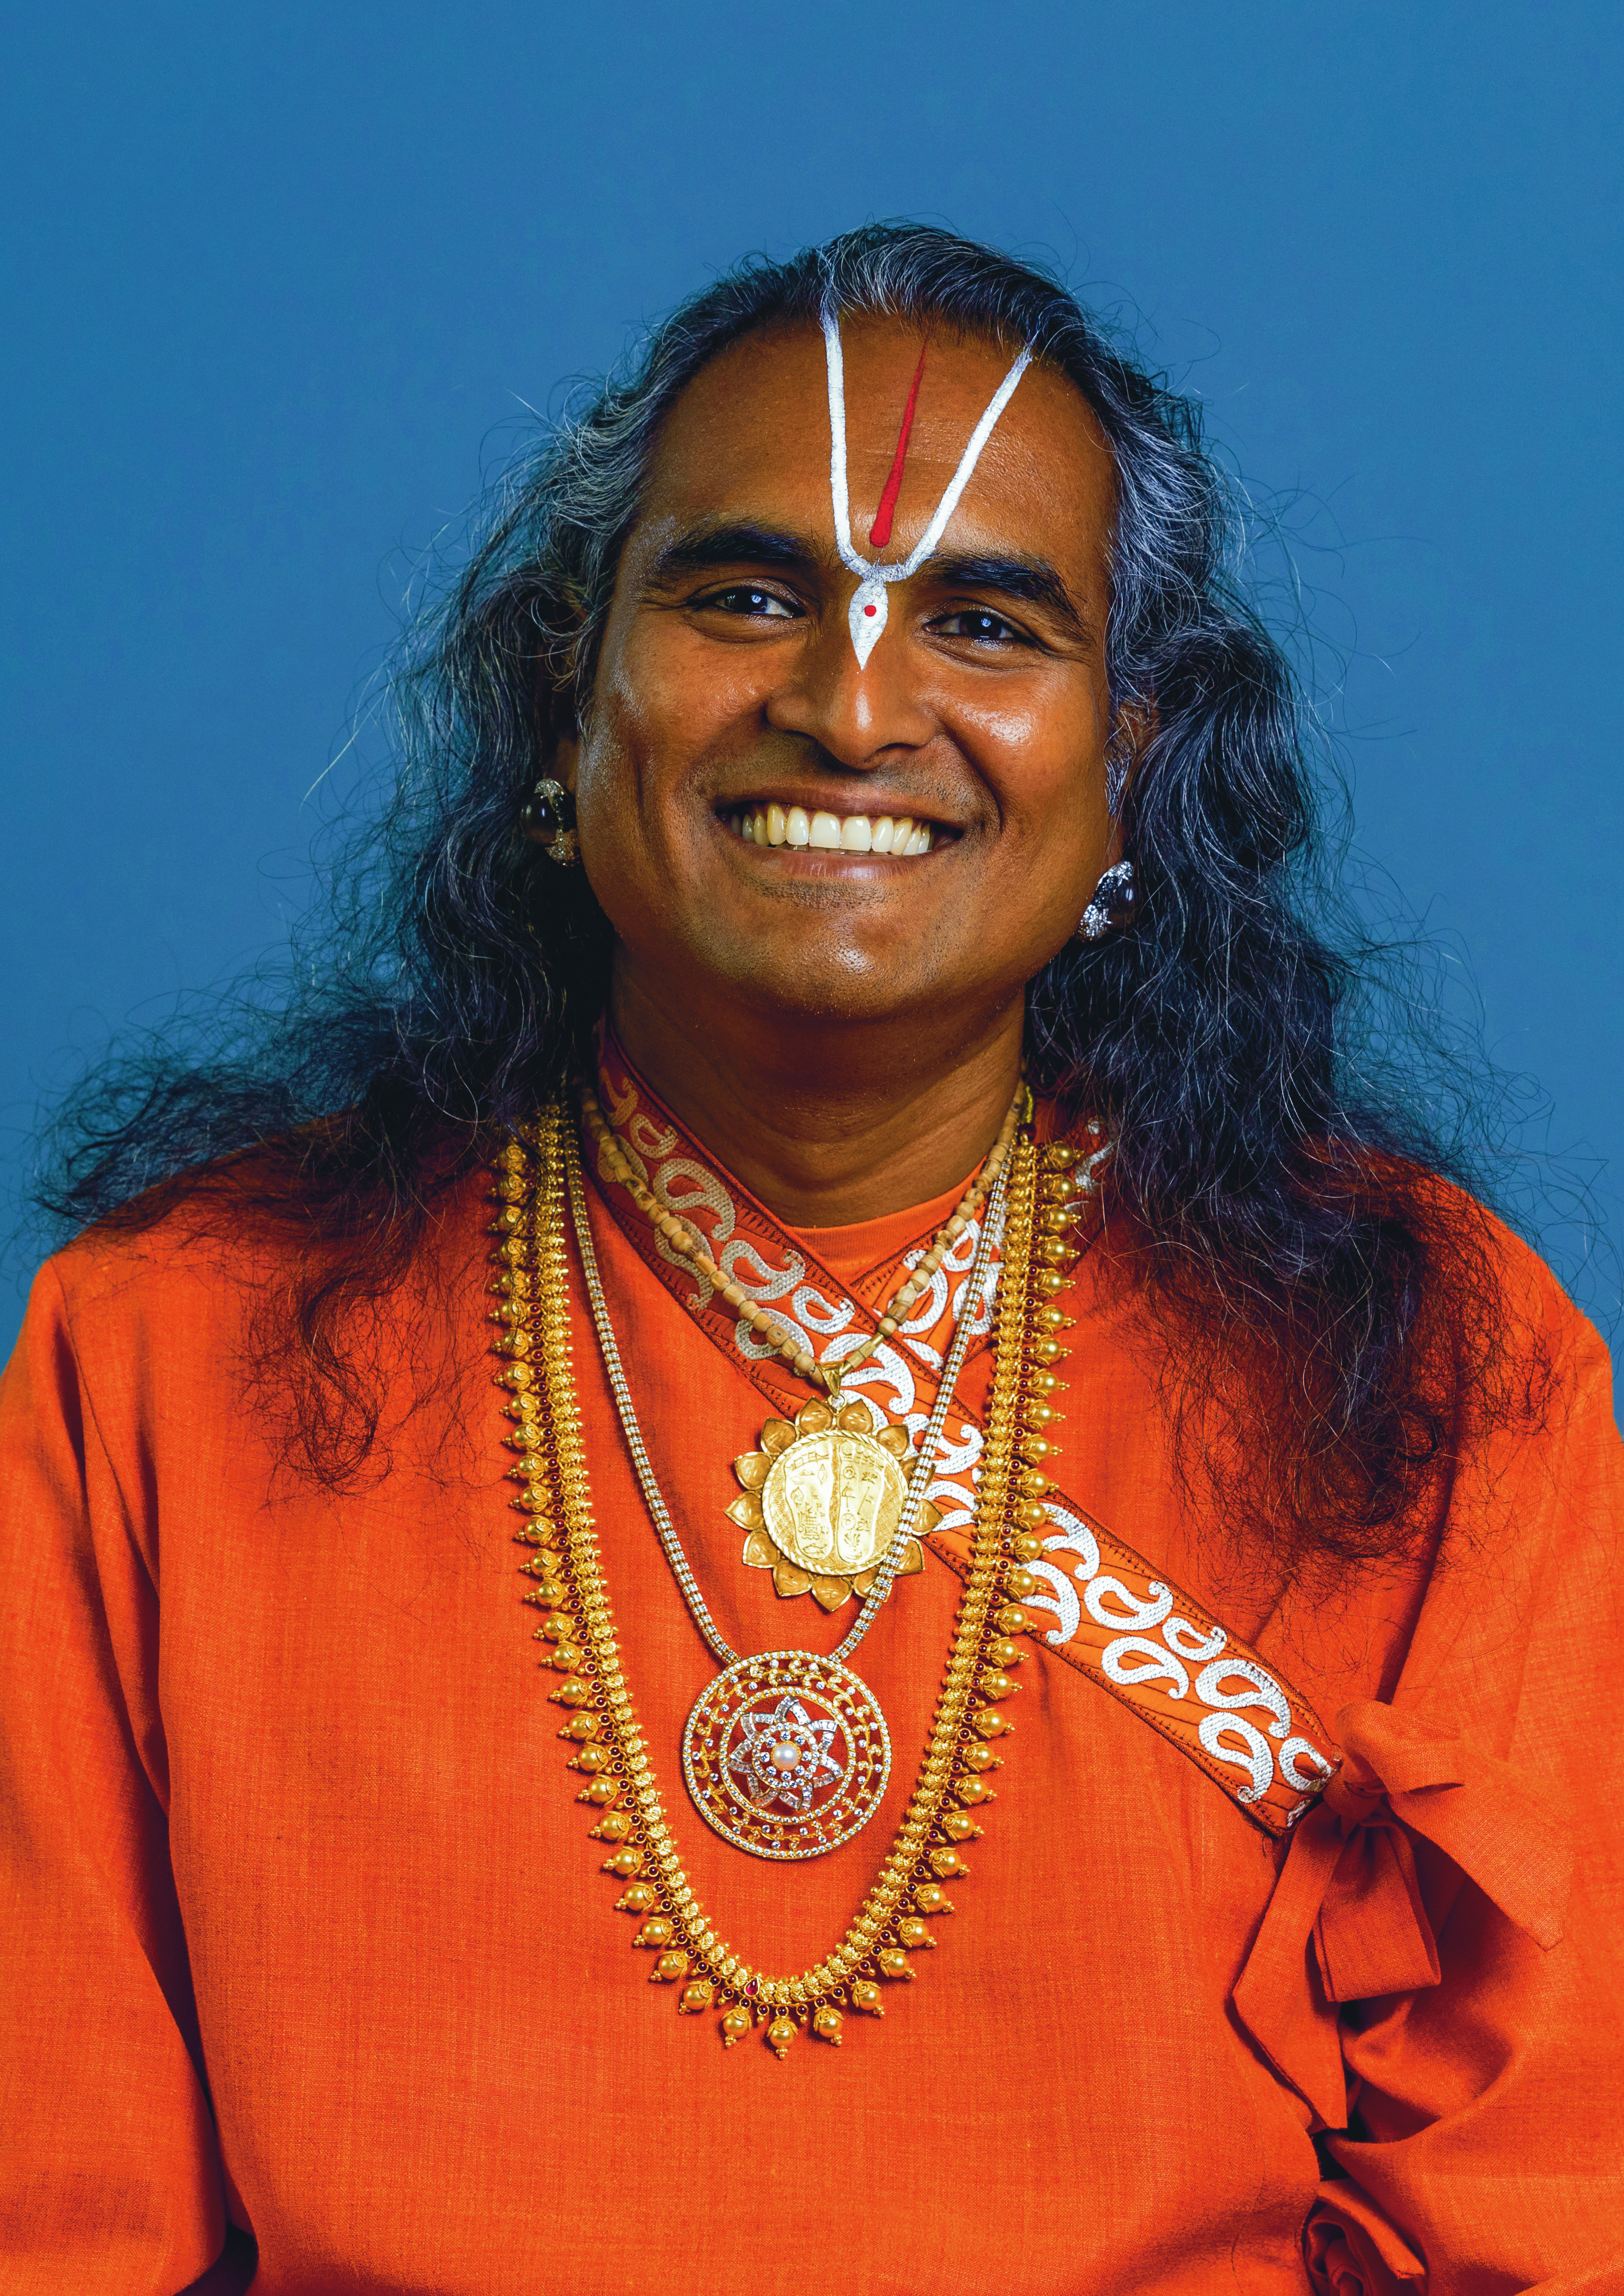
\includegraphics[width=0.9\textwidth]{assets/imgs/Guruji_cmyk.jpg} 

\vspace*{0.5cm}

\begin{minipage}[t]{0.8\textwidth}\fontsize{12pt}{14pt}\selectfont
This work is dedicated to Paramahamsa Vishwananda, founder of the Hari Bhakta Sampradāya and \textit{satguru} for those who take His shelter. 
\end{minipage}


\end{center}
\include{misc/blank_page}
\thispagestyle{empty} % No header or footer

\vspace*{1cm} % Top spacing for balanced layout

\begin{center}
    {\large\itshape
    śrīmat paraṁ brahma guruṁ smarāmi \\
    śrīmat paraṁ brahma guruṁ bhajāmi \\
    śrīmat paraṁ brahma guruṁ vadāmi \\
    śrīmat paraṁ brahma guruṁ namāmi \par
    }

    \vspace{1em}

    \small
    I remember my \textit{guru} who is Parabrahman; \\
    I worship my \textit{guru} who is Parabrahman; \\
    I praise my \textit{guru} who is Parabrahman; \\
    I bow to my \textit{guru} who is Parabrahman.

    \vspace{2em}

    {\large\itshape
    namāmi nārāyaṇa-pāda-paṅkajaṁ \\
    karomi nārāyaṇa-pūjanaṁ sadā \\
    vadāmi nārāyaṇa-nāma nirmalaṁ \\
    smarāmi nārāyaṇa-tattvam avyayam \par
    }

    \vspace{1em}

    \small
    At every moment I bow to the lotus feet of Nārāyaṇa, \\
    I worship Nārāyaṇa, I recite the pure Names of Nārāyaṇa, \\
    and I meditate on the changeless truth of Nārāyaṇa.

    \vspace{2.5em}

    {\large\itshape
    śrī viṭṭhala giridhāri parabrahmaṇe namaḥ \par
    }

    \vspace{1em}

    \small
    My obeisances to the Supreme Lord Viṭṭhala, \\
    who is the refuge and protection of everyone.
\end{center}

\newpage
\thispagestyle{empty}

\vspace*{\fill}
{\footnotesize
\noindent
\begin{flushleft}
  \textbf{Bhagavad Gītā Essentials Second Edition} \\[1em]

  Copyright © 2020--2025 Bhakti Event GmbH \\[1em]

  All international rights reserved. No part of this publication may be reproduced, distributed, or transmitted in any form without the prior written permission of the publisher, except in the case of brief quotations embodied in critical reviews and certain other non-commercial uses permitted by copyright law. \\[1em]

  Publisher: Bhakti Marga Publications \\[1em]

  English, Fifth Edition \\[1em]

  ISBN: 978-3-96343-129-6 

  Cover Art: Paramahamsa Vishwananda \\[1em]

  Bhakti Marga Publications \\
  Am Geisberg 1–8, \\
  65321 Heidenrod–Springen, \\
  Germany \\[1em]

  publications@bhaktimarga.org \\
  publications.bhaktimarga.org
\end{flushleft}
}

\maketitle

\newpage
\thispagestyle{empty} % Set the current page style to empty


\frontmatter
\pagestyle{frontplain} 
\aliaspagestyle{chapter}{frontplain} % use frontplain at chapter openings in frontmatter

\tableofcontents*

% \chapter{Preface to the Second Edition}\label{chap-preface-to-the-second-edition}
\bigskip

% TODO
% keeping the epithets of Arjuna and Krishna

This second edition of the \textit{Bhagavad Gītā Essentials} presents a thoroughly revised text. As such, the Sanskrit transliterations have been carefully standardized according to IAST conventions. 

While the translations of the previous version were based on the \textit{Śrīmad Bhagavad Gītā} with \textit{Gītā-bhāṣya} of Bhagavad Rāmānujācārya, 2013, by U. Ve. Sri Rama Rāmānuja Achari, the verse translation found in this edition has mostly been retranslated from scratch, with the goal of offering up a translation that is more in line with Tādātmya Vedānta, the philosophy of the Hari Bhakta Sampradāya. 

These revisions seek to provide readers and students with a more literal yet approachable and philosophically sound 
text suitable for study and reflection. 

--Bhakti Marga Knowledge Team



% 
% \chapter{Foreword}\label{chap-foreword}
\bigskip
 
Thousands of years ago, in the middle of chaos, uncertainty, and fear on an enormous battlefield, supreme knowledge was given to humanity. We know it now as the \textit{Bhagavad Gītā}. 

The \textit{Gītā} is a narrative between God and a conflicted warrior named Arjuna. The Supreme Lord, in the form of Kṛṣṇa, plays the humble role of a charioteer who masterfully instructs Arjuna about the profound mysteries of life. 

The truth is, the world we are living in today is the same battlefield Arjuna found himself on. The only difference is that the battle each one of us faces is not on the outside, but on the inside. 

In the face of these trials, we need a source of greater wisdom to help us overcome the devastating impact on our thinking, emotions, and reactions. Fortunately for us, Kṛṣṇa’s instructions have stood the test of time and provide the knowledge to help us triumph over the obstacles we face. 

Paramahamsa Vishwananda’s commentary on Kṛṣṇa’s teachings opens up and applies the wisdom of the \textit{Bhagavad Gītā} to our lives today. Ultimately, it helps us understand that we have a relationship with God, and that the goal of life is to become fully aware of that divine connection. 

If we can integrate the teachings of the \textit{Bhagavad Gītā} and Paramahamsa Vishwananda’s commentary in this way, we will begin a uniquely personal journey that takes us from the mind to the heart. And, despite the challenges along the way, it is the guidance of the \textit{guru} that can help us to walk it with trust and courage. 

--SC
% \chapter{The Seeker's Journey}\label{chap-the-seeker-s-journey}
\bigskip

There are some who think that life is totally random or must be explainable by science to be valid. There are others who sense there is something more, something with divine meaning and purpose. Ultimately, however, everyone just wants to be loved and to experience lasting happiness.

To do this, most of us try to maximize pleasures and minimize discomforts through the material world. Many seek fulfillment in relationships or careers. Others turn to sex, drugs, food, shopping, or thrill-seeking to feel alive. The problem is, these desires naturally fuel a drive to accumulate more and more, attempting to fill the void felt inside.

Unfortunately, even the hard-earned happiness gained from these endeavors fades with time. Despite one’s best efforts, the results often leave people feeling empty, disillusioned, and even depressed. Others simply find themselves questioning if this is really all there is to life.

Realizing that the empty promises of the material world cannot satisfy all their needs, many embark on a spiritual journey in search of the only source of real, unconditional love: a relationship with God.


% \chapter{About Paramahamsa Vishwananda}\label{chap-about-paramahamsa-vishwananda}

\bigskip

In our modern times, human beings often live lives of profound ignorance---mistaking the body and mind for the self, oblivious to their own divine essence, and losing awareness of their eternal relationship with God. But the \textit{Bhagavad Gītā} compassionately reveals the way out of this delusion. In verse 4.34, Lord Kṛṣṇa instructs:

\begin{customquote}\fontsize{10}{11}\selectfont
\textit{Learn such wisdom by submission, extensive inquiry, and service from a spiritual master. Such realized beings will impart it to you, for they directly perceive the Truth.}
\end{customquote}

It is the duty of these realized beings, who have directly seen the Truth (\textit{tattva-darśīs}), to guide others from ignorance to awakening. Paramahamsa Vishwananda is such a being---a \textit{satguru}, a spiritual master whose life and teachings embody and exemplify this divine Truth.

Rooted in traditional \textit{bhakti-yoga}, the path of loving devotion, Paramahamsa Vishwananda’s mission is to open the hearts of mankind to the love of God in our modern times.  He reminds us that spirituality is not just a complimentary part of our lives; rather it is their very foundation---to be lived and expressed in every moment. All genuine spiritual practices, rituals, and knowledge lead us beyond the confines of ego and mind, awakening a living, breathing relationship with an infinite, blissful, and loving God.

As a Vaiṣṇava \textit{ācārya} and true \textit{satguru}, Paramahamsa Vishwananda has established the Hari Bhakta Sampradāya---a lineage and home for all devotees (\textit{bhaktas}) of Śrī Hari, the Supreme Lord. This living tradition unmistakably carries His grace and guidance, revealing the glory of the Lord in a unique and personal way. His profound compassion, humor, and humility bring the highest truths down to earth, so that a path traditionally pursued by the few can truly feel accessible to all.

For those who wish to connect with Him, Paramahamsa Vishwananda shares His wisdom through His books, teachings, spiritual practices, live \textit{satsaṅgas} (discourses), Darshan blessings, pilgrimages and His worldwide organization, Bhakti Marga---\enquote{the path of devotion}

\bigskip

\noindent Connect with Him.

\noindent\textbf{https://linktr.ee/paramahamsa\_vishwananda}

\bigskip
\begin{center}
    \qrcode[height=2.5cm]{https://linktr.ee/paramahamsa_vishwananda}
\end{center}

% \chapter{About This Bhagavad Gītā}\label{chap-about-this-bhagavad-gita}

It is rare when a book has the potential to become a lifelong spiritual companion. \textit{Bhagavad Gītā Essentials} is designed to be just that: an essential part of your life. Small enough to carry with you wherever you go, yet profound enough to carry you all the way to God. It is succinct enough to read in a matter of hours, yet deep enough to contemplate for decades to come. 

\textit{Bhagavad Gītā Essentials} evolved out of two live discourses given by Paramahamsa Vishwananda: an 18-day course in 2014 and an 8-day course in 2016. The essence of these commentaries has been distilled to reveal the deeper meaning of this timeless scripture. All 701 Sanskrit verses of the \textit{Bhagavad Gītā} are presented herein along with translations that are infused with the beauty of \textit{bhakti}: love and devotion for God. 

In addition, this \textit{Bhagavad Gītā} has been specially designed to help you get the most out of its verses and commentary:
\begin{itemize}[itemsep=1pt, topsep=6pt]
    \item Each chapter begins with highlights of the knowledge it contains and introduces key points to help you navigate your own journey.

    \item Within each chapter, the verses are grouped together under titles which help you stay connected to its themes.

    \item Finally, definitions of key Sanskrit terms have also been included at the end of each chapter to help you better understand the philosophy behind the verses and commentaries.
\end{itemize}

\section{How to Savor this Bhagavad Gītā}\label{sec-how-to-savor-this-bhagavad-gita}

The \textit{Bhagavad Gītā} offers a most precious treasure: the timeless discourse of Lord Kṛṣṇa which Paramahamsa Vishwananda’s commentary unravels and delivers straight to the heart. 

What you do with it depends on the value you give it. Receiving the Gītā with this in mind allows you to draw on its wisdom in the most powerful way. There are many ways you can savor this scripture: 

\begin{itemize}[itemsep=1pt, topsep=6pt]

\item Reading it cover to cover gives you an overview of the entire scripture. 

\item Reading only the verses from beginning to end allows you to stand next to Arjuna and take direct instruction from the Lord Himself. 

\item Concentrating on the introductory text and commentaries of each chapter helps you discover the secrets hidden within the verses. 

\item Simply letting the Bhagavad Gītā fall open to any page allows the Divine to reveal something to you in the moment. Take it as a gift and contemplate on what you find. 

\end{itemize}

Whether you read a verse a day, a chapter a week, the verses alone, only the commentary, or you just open the Bhagavad Gītā to see what will be revealed to you in the moment, you’ll surely want to keep it close at hand and make it a part of your daily life.

\section{Special Note from Paramahamsa Vishwananda}\label{sec-special-note-from-paramahamsa-vishwananda}

\enquote{The \textit{Bhagavad Gītā} is not a novel. It's not just a book which you read whenever you have time. You have to soak your mind with it. Not only reading it one time.}

\enquote{You have to dive into it, because each line of the \textit{Bhagavad Gītā}, each phrase which Kṛṣṇa has uttered, has a deeper meaning in your life. It’s not outside of your life. He didn’t say something alien to you. Actually, what He has spoken 5000 years ago is still relevant to now. If you see what Arjuna went through, everybody goes through the same thing. That’s why you have to dive into it. Read it one time, two times, three times, hundreds of times. Become a living and walking \textit{Bhagavad Gītā}.}
% \include{frontmatter/7_introduction}

\mainmatter     
\pagestyle{maindocpagestyle}
\aliaspagestyle{chapter}{alternating}
\chapter{Arjuna-viṣāda-yoga}\label{chap-arjuna-visada-yoga}
\chaptersubtitle{The Lamentation of Arjuna}
%%%%%%%%%%%%%%%%%%%%%%%%%%%%%%%%%%%%%%%%%%%%%%%%%%%%%%%%%

\noindent The \textit{Gītā} begins with a vivid description of the scene on the Kurukṣetra battlefield. Key warriors on both sides are named. The blowing of conches and the beating of drums signal the start of this terrible war. It is at this point that the focus shifts to Arjuna and Kṛṣṇa. Eager to assess the enemy ranks, Arjuna asks Kṛṣṇa to take him to the middle of the battlefield so he can take a closer look at those he is about to fight.

Among the opposing army, he sees relatives, friends, and revered elders. The sight of those who were once so dear to him causes Arjuna to lose his resolve. He can no longer see the point in engaging in this battle which will inevitably destroy his family. Confused about his duty and overwhelmed with compassion for his enemies, he begins to pour out his heart to Kṛṣṇa. Surely, he argues, this war cannot be based on righteousness. He repeatedly makes the point that killing one’s own family for the sake of a kingdom will only produce dire consequences for the future. After making his case, the chapter ends with Arjuna casting aside his bow in grief.

\section{Verse 1: Dhṛtarāṣṭra's Inquiry}\label{sec-verse-1-dhrtarastra-s-inquiry}

\Verse[1.1]
{\hspace*{1em}dhṛtarāṣṭra uvāca \\
dharma-kṣetre kuru-kṣetre samavetā yuyutsavaḥ \\
māmakāḥ pāṇḍavāś caiva kim akurvata sañjaya}
{\hspace*{1em}Dhṛtarāṣṭra said: \\
O Sañjaya, having gathered on the holy field of Kurukṣetra, eager for battle, what did my sons and the Pāṇḍavas do?}

\enquote{This verse starts with the word \enquote{\textit{dharma-kṣetra}.} \enquote{\textit{Dharma}} means righteous, \enquote{\textit{kṣetra}} means the field---so this is the field of righteousness.}

\enquote{One of the meanings of this war is life, where the \enquote{good} side fights with the \enquote{not good} side. This war is not outside, it is also happening inside the human body. Your physical body is the \textit{dharma-kṣetra}. You have incarnated to do your \textit{dharma} (duty) in this field.}

\enquote{Life is also a \textit{dharma-kṣetra}. You have come to fulfill your divine purpose. When you are in tune with your true Self, you realize your purpose in life\ldots and that’s what the word \enquote{\textit{dharma-kṣetra}} is reminding you of. Do your \textit{dharma}! Awaken! This \textit{dharma} can be done with the greatest gift which God has given: this field, this body. And when you start doing your \textit{dharma}, you’ll get good merit! But, if you run away from your \textit{dharma}, then you turn towards the dark side.}

\enquote{This blind king, Dhṛtarāṣṭra, represents the mind---the mind which is blind and wants to always stay blind. The mind is hanging on to the outside so much that it has power only when it is focused on something exterior: on the material, on relationships, on gaining this or that. This is the nature of the mind. The mind is blind.}

\enquote{Both families were from the Kuru dynasty. But the king refused to recognize the Pāṇḍavas. The mind doesn’t recognize the good qualities which are present in oneself. The mind can only look towards the senses, looking always towards the outside. The Self, and the positive qualities which are present inside, are not comprehended by it.}

\section{Verses 2-13: The Warriors are Introduced}\label{sec-verses-2-13-the-warriors-are-introduced}


\Verse[1.2]
{\hspace*{1em}sañjaya uvāca \\
dṛṣṭvā tu pāṇḍavānīkaṁ vyūḍhaṁ duryodhanas tadā \\
ācāryam upasaṅgamya rājā vacanam abravīt}
{\hspace*{1em}Sañjaya said: \\
Having seen the Pāṇḍava army arranged in military formation, Duryodhana then approached his teacher Droṇa and spoke these words:}


\Verse[1.3]
{paśyaitāṁ pāṇḍu-putrāṇām ācārya mahatīṁ camūm \\
vyūḍhāṁ drupada-putreṇa tava śiṣyeṇa dhīmatā}
{O teacher, behold this mighty army of the Pāṇḍavas, arrayed by the son of Drupada, your intelligent disciple.}

\Verse[1.4]
{atra śūrā maheṣv-āsā bhīmārjuna-samā yudhi \\
yuyudhāno virāṭaś ca drupadaś ca mahā-rathaḥ}
{In that army are heroes and great archers, equal to Bhīma and Arjuna in battle; there are mighty warriors like Yuyudhāna, Virāṭa, and Drupada.}

\Verse[1.5]
{dhṛṣṭaketuś cekitānaḥ kāśirājaś ca vīryavān \\
purujit kuntibhojaś ca śaibyaś ca nara-puṅgavaḥ}
{There are Dhṛṣṭaketu, Cekitāna, and the valiant king of Kāśī, Purujit, Kuntibhoja, and Śaibyā, the best among men.}

\Verse[1.6]
{yudhāmanyuś ca vikrānta uttamaujāś ca vīryavān \\
saubhadro draupadeyāś ca sarva eva mahā-rathāḥ}
{There are the mighty Yudhāmanyu, the strong Uttamaujā, the son of Subhadrā, as well as the sons of Draupadī, all of whom are mighty warriors.}

\Verse[1.7]
{asmākaṁ tu viśiṣṭā ye tān nibodha dvijottama \\
nāyakā mama sainyasya saṁjñārthaṁ tān bravīmi te}
{O best of \textit{brāhmaṇas}, now hear about our distinguished warriors. For your understanding, I shall tell you the leaders of my army.}

\Verse[1.8]
{bhavān bhīṣmaś ca karṇaś ca kṛpaś ca samitiñjayaḥ \\
aśvatthāmā vikarṇaś ca saumadattis tathaiva ca}
{There are yourself, Bhīṣma, Karṇa, the victorious Kṛpa, Aśvatthāmā, Vikarṇa, and the son of Somadatta.}

\Verse[1.9]
{anye ca bahavaḥ śūrā mad-arthe tyakta-jīvitāḥ \\
nānā-śastra-praharaṇāḥ sarve yuddha-viśāradāḥ}
{There are also many other heroes who have offered their lives for my sake, all wielding various weapons and experienced in the art of warfare.}

\Verse[1.10]
{aparyāptaṁ tad asmākaṁ balaṁ bhīṣmābhirakṣitam \\
paryāptaṁ tv idam eteṣāṁ balaṁ bhīmābhirakṣitam}
{This force of our army marshalled by Bhīṣma is immeasurable, while the strength of their army guarded by Bhīma is limited.}

\Verse[1.11]
{ayaneṣu ca sarveṣu yathā-bhāgam avasthitāḥ \\
bhīṣmam evābhirakṣantu bhavantaḥ sarva eva hi}
{Indeed all of you should just guard Bhīṣma, while stationed at all strategic positions in the army.}

\Verse[1.12]
{tasya sañjanayan harṣaṁ kuru-vṛddhaḥ pitāmahaḥ \\
siṁha-nādaṁ vinadyoccaiḥ śaṅkhaṁ dadhmau pratāpavān}
{\hspace*{1em}(Sañjaya said:) \\
The powerful grandsire Bhīṣma, eldest of the Kuru clan, roaring loudly like a lion, blew his conch to incite Duryodhana's cheerfulness.}

\Verse[1.13]
{tataḥ śaṅkhāś ca bheryaś ca paṇavānaka-gomukhāḥ \\
sahasaivābhyahanyanta sa śabdas tumulo ’bhavat}
{Consequently, conches, kettle drums, small and big drums, and horns immediately sounded forth and the sound was terrific.}


\enquote{Duryodhana represents this great pride that is born from the mind. When the mind is very active, one becomes proud of many things: proud of knowledge, proud of what one has.}

\enquote{The army of the Pāṇḍavas was arrayed in a very special formation. Seeing this orderly formation, Duryodhana felt much nervousness and anxiety inside himself. Anxiety appears when one is proud. Even if pride appears very strong on the outside, in reality, it has a lot of weaknesses in it. Why does pride arise? Do you think it is out of strength? No! In reality, pride arises due to the weakness that one has inside. Even if somebody says, \enquote{Ah yes, I am very proud of this and I am very proud of that,} you can feel that this pride is actually weakness. When pride arises, people think, \enquote{Yes, I am very confident!} No. It’s the mind that perceives pride as confidence. In reality, one is running away from something, from the opposite of pride, which is humility. When one is running away from humility, one only appears to be very grand and confident.}

\enquote{When you start on the spiritual path, your pride sees all your good qualities, but then the mind becomes anxious. This pride tries to make you reason, tries to make you go sideways in a cunning way. That’s why Duryodhana rushes to Droṇācārya, the great teacher of both the Kauravas and the Pāṇḍavas.}

\enquote{Droṇācārya represents attachment to the material. He represents the greed in man. Droṇācārya also had good qualities. He was a great teacher of military science. Sometimes he would even advise Bhīṣma. He was the royal guru. But when the pride of Duryodhana saw the greed in Droṇācārya, he said to himself, \enquote{Let me go and feed his greed. Let me corrupt him.}}

\enquote{Then he praises Bhīṣma. Bhīṣma represents the ego. He was very powerful. He was the great-uncle of the Kauravas and the Pāṇḍavas, and was considered the greatest of all in the Kuru dynasty. He was very virtuous. He was a renunciate\ldots   He was very devoted to his parents. He knew about the scriptures. He was devoted to his teachers. Above all, he was very dedicated to God. Due to this, there was a great ego.}

\enquote{The ego makes you think and feel that you are the best among men. You are the most knowledgeable of all. You have knowledge of everything. And that blinds you. Even if you have many good qualities, if you are egoistic, all these good qualities are nothing because it is all self-centered.}

\enquote{Duryodhana continues, \enquote{There are many more heroes who have sacrificed their lives for my sake.} You see, pride has many friends, and most of these friends have qualities similar to him. Because of his arrogance, Duryodhana attracted similar people with similar qualities. Most of these qualities that were supporting him were in the form of his own ninety-nine brothers.}

\enquote{The Kauravas stand for this outside reality which is looking, fighting, always wanting something, but it’s all material, it’s all external, and that brings superficial joy: joy for a very short time and misery for a longer time.}

\enquote{When you start on your spiritual path, you have a battle: you perceive all the negative qualities within more strongly. Sometimes you’ll awaken a quality which has never been there before. But this is the purification that one goes through; this is the Kurukṣetra that you go through, the \textit{dharma-kṣetra} that you go through. You uproot, one by one, all these qualities and transform them. You transform them until finally you have the Love of God that stays. That’s realization! To receive His grace. To manifest His Love and to beam His Love. And that's the duty of each human being.}

\section{Verses 14-20: Kṛṣṇa is Introduced; The Conches are Blown}\label{sec-verses-14-20-krsna-is-introduced-the-conches-are-blown}

\Verse[1.14]
{tataḥ śvetair hayair yukte mahati syandane sthitau \\
mādhavaḥ pāṇḍavaś caiva divyau śaṅkhau pradadhmatuḥ}
{Then Mādhava and the son of Paṇḍu, seated in a great chariot harnessed by white horses, blew their divine conches.}

\Verse[1.15–16]
{pāñcajanyaṁ hṛṣīkeśo devadattaṁ dhanañjayaḥ \\
pauṇḍraṁ dadhmau mahā-śaṅkhaṁ bhīma-karmā vṛkodaraḥ \\
anantavijayaṁ rājā kuntī-putro yudhiṣṭhiraḥ \\
nakulaḥ sahadevaś ca sughoṣa-maṇipuṣpakau}
{Śrī Kṛṣṇa blew His conch, Pāñcajanya, Arjuna blew his conch named Devadatta, and Bhīma, the performer of terrible deeds, blew the great conch Pauṇḍra. King Yudhiṣṭhira, the son of Kuntī, blew his conch Ananta-vijaya, and Nakula and Sahadeva blew their conches Sughoṣa and Maṇi-puṣpaka.}

\Verse[1.17–18]
{kāśyaś ca parameṣv-āsaḥ śikhaṇḍī ca mahā-rathaḥ \\
dhṛṣṭadyumno virāṭaś ca sātyakiś cāparājitaḥ \\
drupado draupadeyāś ca sarvaśaḥ pṛthivī-pate \\
saubhadraś ca mahā-bāhuḥ śaṅkhān dadhmuḥ pṛthak pṛthak}
{The great archer, king of Kāśī and the mighty warrior Śikhaṇḍī, Dhṛṣṭadyumna, Virāṭa, and the invincible Sātyaki, King Drupada, the sons of Draupadī, and the strong-armed son of Subhadrā, all blew their respective conches.}

\Verse[1.19]
{sa ghoṣo dhārtarāṣṭrāṇāṁ hṛdayāni vyadārayat \\
nabhaś ca pṛthivīṁ caiva tumulo ’bhyanunādayan}
{That tumultuous sound, reverberating through heaven and Earth, tore apart the hearts of Dhṛtarāṣṭra’s sons.}

\Verse[1.20]
{atha vyavasthitān dṛṣṭvā dhārtarāṣṭrān kapi-dhvajaḥ \\
pravṛtte śastra-sampāte dhanur udyamya pāṇḍavaḥ \\
hṛṣīkeśaṁ tadā vākyam idam āha mahī-pate}
{Then, O king, having seen the sons of Dhṛtarāṣṭra arranged in formation, the son of Pāṇḍu, who had Hanumān on his banner, took up his bow in preparation for the clash of weapons. He then spoke these words to Hṛṣīkeśa.}


\enquote{Kṛṣṇa is seated in His chariot holding the reins, controlling the five horses. He is the Controller of all. Arjuna is seated with Him in the chariot and they blow their divine conches. This denotes that when one shows interest in changing, when the Lord perceives that one is making an effort to change, then the Lord Himself gives strength, power, energy and faith to that person who is willing to change. He gives one power to control the senses: the five horses pulling the chariot represent the five senses.}

\enquote{Imagine all these people blowing conches: so powerful and so strong must have been this sound at that time, that everything around started to tremble! And not only there on the battlefield, but also in the heavens. It didn’t happen just in this physical world. It also happened in the spiritual world.}


\enquote{They used the conch to announce the beginning and the end of war. The sound is \textit{oṁ}. This sound which vibrates, shows that at the end, no matter how big the battle is, how strong or difficult it is, one finds one’s way. At the end, everything resounds in the cosmic sound. At the end, it is through this cosmic sound that one attains realization. This cosmic sound is the word of God Himself. The conch and the bell are not just mere instruments. When one blows the conch, it awakens the divinity inside. It awakens clarity inside. It vibrates and the vibration also vibrates in your brain. The same is true of the bell.}

\enquote{When you go with full force on your spiritual path, nothing can move you! Nothing that people can say, nothing that people can do, can make you move from your path. That’s what Christ says about having faith. About building your faith on a rock so that nothing can move you! If you build your house on sand, it will break. If you build your house on a rock, it will be very strong. This sound that we are talking about is the inner strength. When you have inner strength, it’s not only in your heart. Your whole being will be full of energy! From head to toe, you’ll be full of energy, because that energy is not from the outside, it is from deep within. This energy is from God Himself, from Kṛṣṇa Himself, and it beams out and gives you the support and the strength to move forward. But you should not look at your weakness, even if you see the weakness. It is part of you, yes! But hang onto your strength!}

\newpage
\section{Verses 21-25: Between the Two Armies}\label{sec-verses-21-25-between-the-two-armies}

\Verse[1.21–22]
{\hspace*{1em}arjuna uvāca \\
senayor ubhayor madhye rathaṁ sthāpaya me ’cyuta \\
yāvad etān nirīkṣe ’haṁ yoddhu-kāmān avasthitān \\
kair mayā saha yoddhavyam asmin raṇa-samudyame}
{\hspace*{1em}Arjuna said: \\
O Acyuta, station my chariot between both armies until I may see those standing near, eager for combat and with whom I must fight in this impending battle.}

\Verse[1.23]
{yotsyamānān avekṣe ’haṁ ya ete ’tra samāgatāḥ \\
dhārtarāṣṭrasya durbuddher yuddhe priya-cikīrṣavaḥ}
{I wish to see those who have gathered here and will fight in battle, wishing to please the evil-minded son of Dhṛtarāṣṭra}

\Verse[1.24–25]
{\hspace*{1em}sañjaya uvāca \\
evam ukto hṛṣīkeśo guḍākeśena bhārata \\
senayor ubhayor madhye sthāpayitvā rathottamam \\
bhīṣma-droṇa-pramukhataḥ sarveṣāṁ ca mahī-kṣitām \\
uvāca pārtha paśyaitān samavetān kurūn iti}
{\hspace*{1em}Sañjaya said: \\
O descendant of Bharata, having thus been addressed by Guḍākeśa, Hṛṣīkeśa stationed that best of chariots between the two armies. In front of Bhīṣma, Droṇa, and all the other kings, He said: \enquote{O Pārtha, behold all the Kurus who have assembled here.}}

\enquote{Arjuna said to Kṛṣṇa, \enquote{move my chariot in between.} So, this \enquote{in-between state} stands for neutral. You are neither on one side, nor the other. You are neither on the good side, nor on the bad side. For you to be able to observe, you have to be in that neutral state, that neutral point. Very often people take decisions in life being on one side. If you are on one side, there is always judgment, there is always confusion.}

\enquote{Testing times may arise in the form of troubles. Often one doesn’t want to go through it, and so one tries to bypass it, and go sideways. But life is like this. Life is a great lesson. If you don’t face your problem, if you don’t face your negative quality and look at it in the eyes, you’ll never become strong. If you always try to go sideways, you will not learn anything. Arjuna says, \enquote{Place me between them. Let me see---face to face, eye to eye---what are these qualities, what is this pain. Let me go above it, rise over, master it! I wish to see who I am to fight.} Here it is not about fighting, it is about transcending. \enquote{What will I transcend? Which quality?} This is self-analysis. This is the point where Arjuna is analysing. Arjuna here represents self-observance. Observe all your qualities---your \enquote{good} qualities and your \enquote{not good} qualities---and then you can know how to overcome them, transcend them and transform them.}

\section{Verses 26-47: Arjuna Refuses to Fight}\label{sec-verses-26-47-arjuna-refuses-to-fight}
\Verse[1.26–27]
{tatrāpaśyat sthitān pārthaḥ pitṝn atha pitāmahān \\
ācāryān mātulān bhrātṝn putrān pautrān sakhīṁs tathā \\
śvaśurān suhṛdaś caiva senayor ubhayor api}
{Pārtha saw standing there, fathers and grandfathers,
teachers, maternal uncles, brothers, sons, grandsons and friends, as well as fathers-in-law and well-wishers among both armies.}

\Verse[1.27–28]
{tān samīkṣya sa kaunteyaḥ sarvān bandhūn avasthitān \\
kṛpayā parayāviṣṭo viṣīdann idam abravīt}
{Having seen all his friends and relatives there, Kaunteya became filled with deep compassion and grievingly spoke these words:}

\Verse[1.28–29]
{\hspace*{1em}arjuna uvāca \\
dṛṣṭvemaṁ sva-janaṁ kṛṣṇa yuyutsuṁ samupasthitam \\
sīdanti mama gātrāṇi mukhaṁ ca pariśuṣyati \\
vepathuś ca śarīre me roma-harṣaś ca jāyate}
{\hspace*{1em}Arjuna said: \\
O Kṛṣṇa, after seeing my own family and friends assembled here desiring to fight, my limbs are becoming weak and my mouth is drying up. My body is trembling, and my hair is standing on end.}

\Verse[1.30]
{gāṇḍīvaṁ sraṁsate hastāt tvak caiva paridahyate \\
na ca śaknomy avasthātuṁ bhramatīva ca me manaḥ}
{My bow, the Gāṇḍīva, is slipping from my hands and my skin is burning. I am unable to hold myself together and my mind appears as if reeling.}

\Verse[1.31]
{nimittāni ca paśyāmi viparītāni keśava \\
na ca śreyo ’nupaśyāmi hatvā sva-janam āhave}
{O Keśava, moreover I perceive sinister omens and cannot see any benefit in killing my own family in battle.}

\Verse[1.32]
{na kāṅkṣe vijayaṁ kṛṣṇa na ca rājyaṁ sukhāni ca \\
kiṁ no rājyena govinda kiṁ bhogair jīvitena vā}
{O Kṛṣṇa, neither do I desire victory, the kingdom, or comforts. Of what use to us is a kingdom, enjoyments, or even life itself, Govinda?}

\Verse[1.33–34]
{yeṣām arthe kāṅkṣitaṁ no rājyaṁ bhogāḥ sukhāni ca \\
ta ime ’vasthitā yuddhe prāṇāṁs tyaktvā dhanāni ca \\
ācāryāḥ pitaraḥ putrās tathaiva ca pitāmahāḥ \\
mātulāḥ śvaśurāḥ pautrāḥ śyālāḥ sambandhinas tathā}
{Those for whose sake we desire the kingdom, enjoyments, and comforts stand ready to fight and have given up their lives and wealth for this war---teachers, fathers, sons and also grandfathers, uncles, fathers-in-law and grandsons, brothers-in-law and other relatives.}

\Verse[1.35]
{etān na hantum icchāmi ghnato ’pi madhusūdana \\
api trailokya-rājyasya hetoḥ kiṁ nu mahī-kṛte}
{O Madhusūdana, they may be intent on slaying me, but I have no desire to kill them, even for reign over the three worlds, much less for sovereignty over this Earth.}

\Verse[1.36]
{nihatya dhārtarāṣṭrān naḥ kā prītiḥ syāj janārdana \\
pāpam evāśrayed asmān hatvaitān ātatāyinaḥ}
{After killing the sons of Dhṛtarāṣṭra, what joy would be ours, O Janārdana? Sin alone would stain us if we killed these aggressors.}

\Verse[1.37]
{tasmān nārhā vayaṁ hantuṁ dhārtarāṣṭrān sva-bāndhavān \\
sva-janaṁ hi kathaṁ hatvā sukhinaḥ syāma mādhava}
{Therefore, it is not right that we slay the sons of Dhṛtarāṣṭra, our own relatives. Indeed how can we rejoice, O Mādhava, by killing our kinsmen?}

\Verse[1.38–39]
{yady apy ete na paśyanti lobhopahata-cetasaḥ \\
kula-kṣaya-kṛtaṁ doṣaṁ mitra-drohe ca pātakam \\
kathaṁ na jñeyam asmābhiḥ pāpād asmān nivartitum \\
kula-kṣaya-kṛtaṁ doṣaṁ prapaśyadbhir janārdana}
{Even though these people, whose minds are overpowered by greed, see no vice in destroying their family and betraying their friends, why should we, O Kṛṣṇa, who do recognize this evil of destroying the family, not know to turn away from this evil?}

\Verse[1.40]
{kula-kṣaye praṇaśyanti kula-dharmāḥ sanātanāḥ \\
dharme naṣṭe kulaṁ kṛtsnam adharmo ’bhibhavaty uta}
{Once the family lineage is destroyed, ancient family traditions perish, and when traditions perish, unrighteousness certainly overtakes the whole clan.}

\Verse[1.41]
{adharmābhibhavāt kṛṣṇa praduṣyanti kula-striyaḥ \\
strīṣu duṣṭāsu vārṣṇeya jāyate varṇa-saṅkaraḥ}
{O Kṛṣṇa, from the rise of unrighteousness, the women of the clan become corrupt; when women become corrupt, O descendant of Vṛṣṇi, the mixing of \textit{varṇas} ensues.}

\Verse[1.42]
{saṅkaro narakāyaiva kula-ghnānāṁ kulasya ca \\
patanti pitaro hy eṣāṁ lupta-piṇḍodaka-kriyāḥ}
{This mixing of social classes verily results in hell for the family and for those who destroy it. Consequently, the ancestors of such a family lineage certainly fall due to being deprived of their ritual offerings.}

\Verse[1.43]
{doṣair etaiḥ kula-ghnānāṁ varṇa-saṅkara-kārakaiḥ \\
utsādyante jāti-dharmāḥ kula-dharmāś ca śāśvatāḥ}
{By these sinful deeds of the destroyers of the family lineage which cause the mixing of social classes, the everlasting \textit{dharma} of the society and family traditions are ruined.}

\Verse[1.44]
{utsanna-kula-dharmāṇāṁ manuṣyāṇāṁ janārdana \\
narake niyataṁ vāso bhavatīty anuśuśruma}
{We have heard repeatedly, O Janārdana, that there is inevitably a place in Hell for those whose family traditions are destroyed.}

\Verse[1.45]
{aho bata mahat pāpaṁ kartuṁ vyavasitā vayam \\
yad rājya-sukha-lobhena hantuṁ sva-janam udyatāḥ}
{How unfortunate! We have resolved to commit a great crime by being ready to kill our own family, driven by greed for the pleasures of a kingdom.}

\Verse[1.46]
{yadi mām apratīkāram aśastraṁ śastra-pāṇayaḥ \\
dhārtarāṣṭrā raṇe hanyus tan me kṣemataraṁ bhavet}
{It would be better for me if the sons of Dhṛtarāṣṭra with weapons in their hands were to kill me in battle, unresisting and unarmed.}


\Verse[1.47]
{\hspace*{1em}sañjaya uvāca \\
evam uktvārjunaḥ saṅkhye rathopastha upāviśat \\
visṛjya sa-śaraṁ cāpaṁ śoka-saṁvigna-mānasaḥ}
{\hspace*{1em}Sañjaya said: \\
Having spoken these words on the battlefield, Arjuna threw aside his bow and arrows, and sat down on the seat of his chariot, his mind overwhelmed with grief.}

\enquote{You were born for a reason and that reason is to realize your Self, to awaken the divinity inside of you and to bring it to others; not merely to say, \enquote{Okay, I have a good life.}}

\enquote{You are born with all your negative qualities. They are dormant inside you. Throughout many lifetimes you have carried them with you, but when the time comes for you to remove them, you just sit there and say, \enquote{No, I can’t do it!} The same was true for Arjuna. He is just sitting there saying, \enquote{I can’t do it!,} because he is still holding onto his weaknesses.}

\enquote{Arjuna is overtaken by emotions which will stop him from fighting. So he becomes cowardly, very soft. If you are soft, you can’t help anyone; you have to be strong. Here Kṛṣṇa reminds Arjuna that he will not move forward if he is weak. Yet Kṛṣṇa allows this feeling to awaken in Arjuna because He is purifying him. He is showing him, \enquote{Look at this clearly. It is not outside; it is inside of you. These people who you see outside of you, why do you feel this connection with them? Because they are inside your heart.} These negative qualities that you see outside, in other people, they are not outside: they are inside of you. If you want to transcend them, you have to dig them out from the inside. You have to remove them from deep within. Not just superficially, by the mind saying, \enquote{Ah yes, I have changed, it is finished! Good! Now, God loves me! And I love God!} No, it doesn’t work like that! Because loving God has to come from inside. For Him to manifest Himself, for Him to come to you, to run to you, a great amount of sincerity, strength and power has to be there!}

\enquote{In his confusion, Arjuna tries to find all kinds of excuses not to fight. He sees that Kṛṣṇa is just looking at him, not bothered about these things. Arjuna is using all kinds of words to please Kṛṣṇa, to make Kṛṣṇa agree with him. Like I explained earlier, when one is in a depressed state, one will look to everybody else to acknowledge one’s depression. Arjuna is depressed and trying to make Kṛṣṇa say, \enquote{Poor you! We will not fight.} He is trying to make Kṛṣṇa acknowledge that whatever he is saying is right. He is in a state of deep confusion and the Great Doctor is sitting there with him! Do you think that the Great Doctor would just sit there, start crying with him and say, \enquote{Oh, my God! Oh, Arjuna, you are right, let’s go back!} Not a chance!}

\enquote{Kṛṣṇa is just listening and waiting for Arjuna to finish crying. It is like this in life. If you try to reason with a person who is in this state, it’s of no use. The Lord is just watching and saying, \enquote{Okay, carry on. Do you have more? Send it! I am listening. I am patient.}}

\enquote{In life, your \textit{guru} is always with you, whether you are on the left side or on the right side, but you have to learn to listen. Here, Kṛṣṇa is standing with him in the battle. In the battle of life, the master is with you, helping you to find your way out of this confusion.}

\enquote{This inner confusion which Arjuna is going through, is in all of us\ldots You can’t change the world outside. What you can change is yourself. But the willingness to change must be there. Because if you don’t have the willingness to change, even reading or listening to the \textit{Bhagavad Gītā} will not do anything inside of you. But if you have just a little percentage of that willingness, then the change will happen.}

\enquote{Arjuna is reduced to a very terrible state\ldots In daily life, you see many people who go through that state. But it is a very important state, because in this state you are building your base in spirituality. If you are weak, you can’t stand on the spiritual path. You have to become strong\ldots Don’t look only at the situation; often certain situations happen in life that we don’t want to see. Here Kṛṣṇa is saying, \enquote{Look at it! Face it and go beyond it!}}

\enquote{At the beginning of your spiritual path, it’s not easy. You have to fight that mind.}
\enquote{In this battlefield of life, if you create an illusion to make yourself feel happy, then if anything appears in front of you, you try to find ways to run away from it. This is cowardice, going sideways, \enquote{putting it in a drawer.} You will never be free, because sooner or later you will be facing the same thing again. But once you have faced it, it will never come back to you again.}

%\chapter{Sāṅkhya-yoga}\label{chap-sankhya-yoga}
\chaptersubtitle{The Eternal Nature of the Self}
%%%%%%%%%%%%%%%%%%%%%%%%%%%%%%%%%%%%%%%%%%%%%%%%%%%%%%%%%

\noindent Despite Kṛṣṇa urging Arjuna to shake off his weakness, he continues to express his unwillingness to fight. Eventually, in a helpless state, Arjuna surrenders to Kṛṣṇa and begs for guidance. At this point, Kṛṣṇa assumes the role of the \textit{satguru}\footnote{A \textit{guru} who can grant God-realization by mere will.} and teaches him about the nature of the Self---the \textit{ātmā}\footnote{The individual, eternal, conscious, and blissful Self, distinct from the body-mind complex and yet infusing life into it.} present in every individual. He describes how the \textit{ātmā} is indestructible, eternal, and beyond this material world. Just as we cast off old clothes and adorn ourselves with new ones, the soul sheds old bodies and takes on new ones. As a \textit{kṣatriya} (warrior), therefore, Arjuna should have no reservation in carrying out his duty since ultimately nobody can be killed.

Having established Arjuna in this philosophical understanding, Kṛṣṇa proceeds to teach one of the fundamental concepts of the \textit{Gītā}: \textit{karma-yoga}. He explains that those of small intelligence perform various duties with the hope of gaining some limited reward; this attachment to results is what produces \textit{karma}.\footnote{Any action done with the body or mind that produces further consequences.} But Kṛṣṇa urges Arjuna to carry out his duty as a warrior without any attachment to the results. By engaging in righteous action without any selfish gain, one can be freed from all \textit{karmic} consequences. With the senses restrained and the mind controlled, one is not distracted by the ways of the world. In this desire-less state, a \textit{yogī} achieves perfect wisdom and peace.

This overview of \textit{karma-yoga}\footnote{The path by which one continues to act in the world with detachment. Such acts, therefore, do not create further consequences.
} provides the centerpiece for Kṛṣṇa's teachings over the next four chapters. We learn about the real meaning of action, what is true renunciation, as well as the ultimate state that is reached when practicing this \textit{yoga}.

\section{Verses 1-9: Arjuna Seeks Refuge in Kṛṣṇa as the Guru}\label{sec-verses-1-9-arjuna-seeks-refuge-in-krsna-as-the-guru}

\Verse[2.1]
{\hspace*{1em}sañjaya uvāca \\
taṁ tathā kṛpayāviṣṭam aśru-pūrṇākulekṣaṇam \\
viṣīdantam idaṁ vākyam uvāca madhusūdanaḥ}
{\hspace*{1em}Sañjaya said: \\
To Arjuna, who was thus despondent and overwhelmed with pity, his eyes filled with confusion and tears, Madhusūdana spoke these words:}

\Verse[2.2]
{\hspace*{1em}śrī-bhagavān uvāca \\
kutas tvā kaśmalam idaṁ viṣame samupasthitam \\
anārya-juṣṭam asvargyam akīrti-karam arjuna}
{\hspace*{1em}Bhagavān Kṛṣṇa said: \\
O Arjuna, from where has this weakness come in this hour of danger? It is unworthy of noble persons and will not lead to the attainment of Heaven. Instead, it causes dishonor.}

\Verse[2.3]
{klaibyaṁ mā sma gamaḥ pārtha naitat tvayy upapadyate \\
kṣudraṁ hṛdaya-daurbalyaṁ tyaktvottiṣṭha parantapa}
{Do not give in to this cowardice, O Arjuna, it does not befit you. Throw away this lowly weakness of heart and arise, O vanquisher of enemies!}

\Verse[2.4]
{\hspace*{1em}arjuna uvāca \\
kathaṁ bhīṣmam ahaṁ saṅkhye droṇaṁ ca madhusūdana \\
iṣubhiḥ pratiyotsyāmi pūjārhāv ari-sūdana}
{\hspace*{1em}Arjuna said: \\
O Madhusūdana, destroyer of enemies, how can I fire arrows against Bhīṣma and Droṇa in battle, who are worthy of worship?}

\Verse[2.5]
{gurūn ahatvā hi mahānubhāvān \\
śreyo bhoktuṁ bhaikṣyam apīha loke \\
hatvārtha-kāmāṁs tu gurūn ihaiva \\
bhuñjīya bhogān rudhira-pradigdhān}
{It would be better to live in this world, even by begging, than to kill these noble, venerable elders. Our enjoyment of avaricious pleasures, after killing them here, would certainly be stained with blood.}

\Verse[2.6]
{na caitad vidmaḥ kataran no garīyo \\
yad vā jayema yadi vā no jayeyuḥ \\
yān eva hatvā na jijīviṣāmas \\
te ’vasthitāḥ pramukhe dhārtarāṣṭrāḥ}
{We do not know which of the two is better for us---defeating them or being conquered by them. Those sons of Dhṛtarāṣṭra after killing whom we would no longer wish to live, are verily standing here before us.}

\Verse[2.7]
{kārpaṇya-doṣopahata-svabhāvaḥ \\
pṛcchāmi tvāṁ dharma-sammūḍha-cetāḥ \\
yac chreyaḥ syān niścitaṁ brūhi tan me\\
śiṣyas te ’haṁ śādhi māṁ tvāṁ prapannam}
{With my nature overcome by the stain of weakness and my mind confused about my duty, I urge You to tell me clearly what would be better for me. I am Your disciple who has taken refuge in You. Please instruct me.}

\Verse[2.8]
{na hi prapaśyāmi mamāpanudyād \\
yac chokam ucchoṣaṇam indriyāṇām \\
avāpya bhūmāv asapatnam ṛddhaṁ \\
rājyaṁ surāṇām api cādhipatyam}
{Even the attainment of a prosperous, unchallenged kingdom on this Earth---or lordship over the gods---I cannot see what could remove this grief that dries up my senses.}

\Verse[2.9]
{\hspace*{1em}sañjaya uvāca \\
evam uktvā hṛṣīkeśaṁ guḍākeśaḥ parantapaḥ \\
na yotsya iti govindam uktvā tūṣṇīṁ babhūva ha}
{\hspace*{1em}Sañjaya said: \\
Having thus spoken to Hṛṣīkeśa, Arjuna, the conqueror of sleep and vanquisher of enemies, said to Govinda, \enquote{I will not fight} and became silent.}

\enquote{In the last chapter, we saw how Arjuna feels confused and how depressed he has become, because when the mind is focused and concentrated on the negative, everything becomes negative. We will see how Lord Kṛṣṇa gives Arjuna the knowledge of the \textit{Gītā} and how He starts to talk to Arjuna about the knowledge of the Self.}

\enquote{Kṛṣṇa is a great psychologist; He doesn’t directly go and give Arjuna everything. He goes slowly with him, step by step. He doesn’t change him, but He gradually allows Arjuna to transform himself.}

\enquote{In this chapter, Kṛṣṇa becomes the \textit{guru}. All this time, Arjuna has been looking at Kṛṣṇa as his cousin and his friend. But now, seeing this terrible, pitiful state of Arjuna, Kṛṣṇa starts to teach. At this moment, Kṛṣṇa becomes the \textit{guru} and Arjuna, the disciple. But Arjuna’s willingness to listen to Kṛṣṇa is very important!}

\enquote{How can Kṛṣṇa tell something to Arjuna, if Arjuna doesn’t want to listen? In the first chapter, you saw that Kṛṣṇa doesn’t say much: He keeps quiet and listens to what Arjuna has to say. But when Arjuna is tired of talking, then Kṛṣṇa reveals to him the \textit{Gītā}. Only when you can listen, can you change! If you can’t listen, how will you change? You will never change. Life is like this: if you don’t learn to listen and observe, you will not transform.}

\enquote{The instruction of the \textit{guru} is like a seed which is planted in fertile land. If the disciple’s heart is like a stone, nothing will grow from it.}

\enquote{When a disciple takes refuge in the \textit{guru}, the disciple must completely accept the superiority of the master. This is what Arjuna is accepting.}

\enquote{When you come to the master, you have to come as an empty vessel so that you can be filled. That mind must be emptied to receive. You have to have this willingness to change to have the full benefit.}

\enquote{If you start to think about what you are losing, you will never get anything, because on the spiritual path you may lose everything on the outside, but in reality, you are gaining everything.}

\enquote{Arjuna’s eyes are brightened and his mind is completely transformed. His whole attitude has changed. With folded hands, he knows that by taking this role of the disciple, that the Lord, the God Almighty, the omniscient, and the knower of all hearts, has taken the form of the supreme master. And that He, who is full of Love, greatness, virtue, and knowledge, He who is non-attached, who can’t be touched by \textit{karma} or by anything, is his dear friend. And from being his best friend, He has become the supreme guide and the supreme divinity.}

\enquote{This is the greatness of the \textit{guru}. The \textit{guru} does not have just one role. He is not just a teacher. He takes different forms, a multitude of aspects. Because the life of the \textit{guru} is not for Himself, but for others. The help and support, the knowledge, the power, and the affection that the \textit{guru} has for the devotee, is amazing and exquisite.}

\newpage
\section{Verses 10-30: The Eternal Nature of the Soul}\label{sec-verses-10-30-the-eternal-nature-of-the-soul}

\Verse[2.10]
{tam uvāca hṛṣīkeśaḥ prahasann iva bhārata \\
senayor ubhayor madhye viṣīdantam idaṁ vacaḥ}
{O descendant of Bharata, as he was grieving between the two armies, Hṛṣīkeśa, slightly smiling, spoke the following words to him.}

\Verse[2.11]
{\hspace*{1em}śrī-bhagavān uvāca \\
aśocyān anvaśocas tvaṁ prajñā-vādāṁś ca bhāṣase \\
gatāsūn agatāsūṁś ca nānuśocanti paṇḍitāḥ}
{\hspace*{1em}Bhagavān Kṛṣṇa said: \\
You are grieving for those who should not be grieved for, yet you speak words of wisdom. The truly wise ones lament neither for the dead nor for the living.}

\Verse[2.12]
{na tv evāhaṁ jātu nāsaṁ na tvaṁ neme janādhipāḥ \\
na caiva na bhaviṣyāmaḥ sarve vayam ataḥ para}
{Surely there has never been a time when I didn't exist, nor you, nor any of these kings, nor will there ever be a time when we all don't exist.}

\Verse[2.13]
{dehino ’smin yathā dehe kaumāraṁ yauvanaṁ jarā \\
tathā dehāntara-prāptir dhīras tatra na muhyati}
{Just as childhood, youth, and old age take place in the body, the embodied \textit{ātmā} attains another body at death. A wise person is not bewildered about this.}

\Verse[2.14]
{mātrā-sparśās tu kaunteya śītoṣṇa-sukha-duḥkha-dāḥ \\
āgamāpāyino ’nityās tāṁs titikṣasva bhārata}
{The contact of the senses with their objects, O Kaunteya, gives rise to feelings of cold and heat, pleasure and pain. They come and go and are impermanent, so endure them without being disturbed, O descendant of Bharata.}

\Verse[2.15]
{yaṁ hi na vyathayanty ete puruṣaṁ puruṣarṣabha \\
sama-duḥkha-sukhaṁ dhīraṁ so ’mṛtatvāya kalpate}
{O best of men, the wise person who is unaffected by these, and to whom pain and pleasure are the same, is indeed worthy of immortality.}

\Verse[2.16]
{nāsato vidyate bhāvo nābhāvo vidyate sataḥ \\
ubhayor api dṛṣṭo ’ntas tv anayos tattva-darśibhiḥ}
{There is no existence of the unreal, and there is no non-existence of the real. This is the conclusion regarding these two that is perceived by those who have realized the Truth.}

\Verse[2.17]
{avināśi tu tad viddhi yena sarvam idaṁ tatam \\
vināśam avyayasyāsya na kaścit kartum arhati}
{Know that which pervades this entire body to be indestructible. None can cause the destruction of the imperishable \textit{ātmā}.}

\Verse[2.18]
{antavanta ime dehā nityasyoktāḥ śarīriṇaḥ \\
anāśino ’prameyasya tasmād yudhyasva bhārata}
{The bodies of the eternal, imperishable, and incomprehensible \textit{ātmā} dwelling in the body are said to be perishable. Therefore fight, O descendant of Bharata.}

\Verse[2.19]
{ya enaṁ vetti hantāraṁ yaś cainaṁ manyate hatam \\
ubhau tau na vijānīto nāyaṁ hanti na hanyate}
{One who believes the \textit{ātmā} to be the killer, and one who thinks it can be killed---both do not know; for the \textit{ātmā} neither slays nor is it slain.}

\Verse[2.20]
{na jāyate mriyate vā kadācin \\
nāyaṁ bhūtvā bhavitā vā na bhūyaḥ \\
ajo nityaḥ śāśvato ’yaṁ purāṇo \\
na hanyate hanyamāne śarīre}
{The \textit{ātmā} is never born, nor does it ever die, nor is it the case that once having come to existence it will cease to exist in the future. It is unborn, eternal, everlasting and most ancient. It is not killed when the body is slain.}

\Verse[2.21]
{vedāvināśinaṁ nityaṁ ya enam ajam avyayam \\
kathaṁ sa puruṣaḥ pārtha kaṁ ghātayati hanti kam}
{O son of Pṛthā, if one knows this \textit{ātmā} to be indestructible, unborn, unchanging, and eternal, how and whom does that person kill or cause to be killed?}

\Verse[2.22]
{vāsāṁsi jīrṇāni yathā vihāya \\
navāni gṛhṇāti naro ’parāṇi \\
tathā śarīrāṇi vihāya jīrṇāny \\
anyāni saṁyāti navāni dehī}
{Just as a person who has discarded worn-out clothes puts on new ones, so the embodied \textit{ātmā}, having discarded its worn-out bodies, enters into new ones.}

\Verse[2.23]
{nainaṁ chindanti śastrāṇi nainaṁ dahati pāvakaḥ \\
na cainaṁ kledayanty āpo na śoṣayati mārutaḥ}
{Weapons do not cut the \textit{ātmā}; fire does not burn it, water does not wet it, and wind does not dry it.}

\Verse[2.24]
{acchedyo ’yam adāhyo ’yam akledyo ’śoṣya eva ca \\
nityaḥ sarva-gataḥ sthāṇur acalo ’yaṁ sanātanaḥ}
{It cannot be cut; it cannot be burnt; it cannot be wetted, and it cannot be dried. It is eternal, all-pervading, changeless, immovable, and everlasting.}

\Verse[2.25]
{avyakto ’yam acintyo ’yam avikāryo ’yam ucyate \\
tasmād evaṁ viditvainaṁ nānuśocitum arhasi}
{This \textit{ātmā} is said to be unmanifest, inconceivable, and unchanging. Knowing the \textit{ātmā} in this way, you should therefore no longer grieve.}

\Verse[2.26]
{atha cainaṁ nitya-jātaṁ nityaṁ vā manyase mṛtam \\
tathāpi tvaṁ mahā-bāho nainaṁ śocitum arhasi}
{Even if you consider this \textit{ātmā} to repeatedly go through birth and death, O Arjuna, even then you should not lament.}

\Verse[2.27]
{jātasya hi dhruvo mṛtyur dhruvaṁ janma mṛtasya ca \\
tasmād aparihārye ’rthe na tvaṁ śocitum arhasi}
{Indeed, death is certain for one who is born, and rebirth is certain for one who has died; therefore do not grieve over what is inevitable.}

\Verse[2.28]
{avyaktādīni bhūtāni vyakta-madhyāni bhārata \\
avyakta-nidhanāny eva tatra kā paridevanā}
{O descendant of Bharata! All beings are unmanifest in the beginning, manifest in the middle and unmanifest at death. So why lament over this?}

\Verse[2.29]
{āścarya-vat paśyati kaścid enam \\
āścarya-vad vadati tathaiva cānyaḥ \\
āścarya-vac cainam anyaḥ śṛṇoti \\
śrutvāpy enaṁ veda na caiva kaścit}
{One person sees the \textit{ātmā} as a wonder, likewise another speaks of it as a wonder; yet another hears of it as a wonder. But even after hearing about it, no one really knows it.}

\Verse[2.30]
{dehī nityam avadhyo ’yaṁ dehe sarvasya bhārata \\
tasmāt sarvāṇi bhūtāni na tvaṁ śocitum arhasi}
{The embodied \textit{ātmā} is in the bodies of all, O descendant of Bharata. It is eternal and indestructible, therefore you should not grieve for any living being.}

\enquote{Now is the beginning of the \textit{Gītā}. The real \textit{Gītā} starts with the smile of the Lord. All that came before was just a preparation for this.}

\enquote{When the \textit{guru} sees that the disciple is really ready, He has the same smile! The disciple can ask ten thousand times and the \textit{guru} will give whatever He has to give. But when the disciple is truly ready, even without asking, all will be given. This is the smile that Lord Kṛṣṇa gives to Arjuna. He says, \enquote{Ah! I see that now you are ready.}}

\enquote{The \textit{guru} will not tell you things which will elevate your ego or your pride. He will tell you things which you don’t want to hear. This is how He crushes the pride out of you; He removes that ignorance out of you\ldots He will show you the way. He will polish you, He will help you to control the mind, He will help you to conquer the senses and conquer the mind. He will help you to banish this unhappiness from you, so that automatically through discrimination, through reflection, through analysis, and the true knowledge of the Self, that true happiness, the permanent happiness, awakens inside of you.}

\enquote{If you want true wisdom, know that there is no birth and no death. You are the \textit{ātmā}, you are eternal. For the \textit{ātmā}, there is no beginning, there is no end. So why do you mourn? You have come here to attain a higher reality; you have come here to do a higher work than what you realize. Kṛṣṇa tells Arjuna that the wise never grieve in this way. The one who has the knowledge of the Self, the realized one, knows that the \textit{ātmā} is eternal and that there is no point in mourning or grieving. The wise person knows that God is the embodiment of true knowledge\ldots The wise person knows that it is only Him who is abiding in everything. He is the Self of all. He is the indestructible Absolute.}

\enquote{[Kṛṣṇa says,] \enquote{There was never a time when I did not exist, nor you! As I existed before everything, you were also with Me.} This is the relationship that we have with God. We are always with Him and He is always with us, whether you want it or not. You can be the greatest atheist and you can say God doesn’t exist; it doesn’t bother Him.}

\enquote{You have an identity. You will always have it. You have ever existed with Him. You are never separate from Him. We all existed before our birth, before we manifested here in these bodies, and we will carry on existing long after these bodies have disappeared. That \textit{ātmā} will always live even if everything gets destroyed.}

\enquote{The body goes through recycling, because it’s made of the five elements, and the five elements go back into nature. But the Self remains untouched, unchanged, immutable, indestructible and it is eternal. It is not created. If something is not created, that means it can’t die.}

\enquote{How you see the body is important. It doesn’t mean that now that you have heard that the body is decaying and deteriorating, one shouldn’t care about it. Then realization will not come to you, because this body is the vehicle to attain that realization.}

\enquote{Even the Lord Himself manifests on Earth in a body. But you should not forget about the \textit{ātmā} also. Nowadays people concentrate so much only on the external reality that they forget that they have a soul.}


\enquote{So, awake, my dear soul. Realize your Self. You are the \textit{ātmā}. Stop being in the sleeping state, because in a sleeping state you will not realize anything. You have to be awake to realize your Self.}


\section{Verses 31-38: The Duty of a Warrior}\label{sec-verses-31-38-the-duty-of-a-warrior}

\Verse[2.31]
{sva-dharmam api cāvekṣya na vikampitum arhasi \\
dharmyād dhi yuddhāc chreyo ’nyat kṣatriyasya na vidyate}
{Additionally, considering your personal duty, you should not hesitate, since for a \textit{kṣatriya}, there is nothing more auspicious than a righteous war.}

\Verse[2.32]
{yadṛcchayā copapannaṁ svarga-dvāram apāvṛtam \\
sukhinaḥ kṣatriyāḥ pārtha labhante yuddham īdṛśam}
{O Pārtha, the \textit{kṣatriyas} rejoice when they get such an opportunity for battle. A war that comes of its own accord opens the gates to Heaven.}

\Verse[2.33]
{atha cet tvam imaṁ dharmyaṁ saṅgrāmaṁ na kariṣyasi \\
tataḥ sva-dharmaṁ kīrtiṁ ca hitvā pāpam avāpsyasi}
{But if you do not fight this righteous war, thus turning away from personal duty and honor, you will incur sin.}

\Verse[2.34]
{akīrtiṁ cāpi bhūtāni kathayiṣyanti te ’vyayām \\
sambhāvitasya cākīrtir maraṇād atiricyate}
{Then people will forever speak of your disgrace, and for an honorable man, dishonor is worse than death.}

\Verse[2.35]
{bhayād raṇād uparataṁ maṁsyante tvāṁ mahā-rathāḥ \\
yeṣāṁ ca tvaṁ bahu-mato bhūtvā yāsyasi lāghavam}
{The great warriors will think that you have fled from the battlefield in fear and you will earn the disrespect of those who held you in high esteem.}

\Verse[2.36]
{avācya-vādāṁś ca bahūn vadiṣyanti tavāhitāḥ \\
nindantas tava sāmarthyaṁ tato duḥkha-taraṁ nu kim}
{Moreover, your enemies, ridiculing your ability, will use words which should never be uttered. Indeed what could be more painful than that?}

\Verse[2.37]
{hato vā prāpsyasi svargaṁ jitvā vā bhokṣyase mahīm \\
tasmād uttiṣṭha kaunteya yuddhāya kṛta-niścayaḥ}
{If slain, you shall gain Heaven; if victorious, you shall enjoy the Earth. Therefore, arise, O son of Kuntī, with firm resolve to fight.}

\Verse[2.38]
{sukha-duḥkhe same kṛtvā lābhālābhau jayājayau \\
tato yuddhāya yujyasva naivaṁ pāpam avāpsyasi}
{Considering pleasure and pain, gain and loss, victory and defeat to be the same, prepare yourself for battle. In this way, you will not incur sin.}

\enquote{Kṛṣṇa is saying everybody knows that they are not the body, everybody knows that they are not the mind, they are not the intellect, but yet, they still identify themselves with them. This is due to the lack of true knowledge, lack of true understanding. You have received this knowledge through books; reading wonderful books has given you this insight. You have heard many talks about it, but it has just remained as words which are pleasurable to you. It doesn’t have any effect upon you. You are still running after the external pleasures; you are still running after things that are perishable.}

\enquote{If you are looking at the soul only from the point of view of the mind, do you think that the mind can understand the soul? A mind which is always moving around is \enquote{\textit{cañcala},} \enquote{restless,} dancing and jumping like a monkey, from one thought to the other. How can the mind, which is in constant movement, be still and perceive the unmovable? The mind will always move from one thing to another until one has gone deeply into the \textit{sādhana} (spiritual practice), deeply into meditation and calmed the mind. Only then, will the soul reveal itself. But before that, if the mind is still jumping around, the soul is unknowable.}

\enquote{\enquote{Considering pleasure and pain, gain and loss, victory and defeat to be the same}: Remind yourself that this is all just a game. Take this pair of opposites as being equal. Even if they appear different, they are the same. A wise man should not be completely taken over by joy when something is happening, but just stay calm. And those who are wise don’t complain when there is some trouble. They analyse the situation. They are in a balanced state in both situations: in a happy moment or in an unhappy moment.}

\enquote{When you do your duty in life, accepting what God is giving you to do, it draws you closer and closer to God-realization. By accepting what God is giving you in your daily life, you are opening the gates to receive more. By showing that you are doing your duty by accepting what God gives you in life, you are showing God that you are ready for a greater purpose in this life, for greater work. Kṛṣṇa says, \enquote{If you run away from this, it will not bring you any good. It will hurt you. It will be unrighteous. Especially on such an occasion, where doing this duty will help you open all the doors to Heaven.} He says, \enquote{Accept life. Accept whatever God gives you.}}

\section{Verses 39-53: The Introduction of Karma-yoga}\label{sec-verses-39-53-the-introduction-of-karma-yoga}

\Verse[2.39]
{eṣā te ’bhihitā sāṅkhye buddhir yoge tv imāṁ śṛṇu \\
buddhyā yukto yayā pārtha karma-bandhaṁ prahāsyasi}
{The knowledge which I have taught to you so far is based on Sāṅkhya.\footnote{A philosophy which states that there are two realities: the Puruṣa (Self) and \textit{prakṛti} (matter). Through an analysis of \textit{prakṛti}, one can realize oneself as the Puruṣa, which is utterly distinct from material nature.} Now listen to the teaching concerning \textit{karma-yoga}. O Pārtha, by being endowed with this wisdom, you will escape the bondage of \textit{karma}.}

\Verse[2.40]
{nehābhikrama-nāśo ’sti pratyavāyo na vidyate \\
svalpam apy asya dharmasya trāyate mahato bhayāt}
{On this path, there is no loss of invested efforts nor is there any failure. Even a little practice of this \textit{yoga} saves one from great fear.}

\Verse[2.41]
{vyavasāyātmikā buddhir ekeha kuru-nandana \\
bahu-śākhā hy anantāś ca buddhayo ’vyavasāyinām}
{On this path the resolute intellect is one-pointed, O descendant of Kuru; but the thoughts of the irresolute are many-branched and endless.}

\Verse[2.42–43]
{yām imāṁ puṣpitāṁ vācaṁ pravadanty avipaścitaḥ \\
veda-vāda-ratāḥ pārtha nānyad astīti vādinaḥ \\
kāmātmānaḥ svarga-parā janma-karma-phala-pradām \\
kriyā-viśeṣa-bahulāṁ bhogaiśvarya-gatiṁ prati}
{O Pārtha, those who are unwise delight in the words of the \textit{Vedas}, declaring \enquote{there is nothing superior to this!} Full of desire and with heaven as their goal, such people utter flowery hymns about special rites to gain power and pleasure, which lead to further birth and \textit{karma}.}

\Verse[2.44]
{bhogaiśvarya-prasaktānāṁ tayāpahṛta-cetasām \\
vyavasāyātmikā buddhiḥ samādhau na vidhīyate}
{The intellect of those who cling to pleasure and power and whose minds have been carried away by such flowery speech, cannot be firmly established in single-pointed focus.}

\Verse[2.45]
{trai-guṇya-viṣayā vedā nistrai-guṇyo bhavārjuna \\
nirdvandvo nitya-sattva-stho niryoga-kṣema ātmavān}
{The \textit{Vedas}\footnote{The earliest body of Indian scripture, consisting of the \textit{Ṛg Veda}, \textit{Sāma Veda}, \textit{Yajur Veda}, and \textit{Atharva Veda}, which lay down the fundamental principles of Hinduism.} deal with the three \textit{guṇas},\footnote{The three qualities within \textit{prakṛti} (matter): \textit{sattva} (purity), \textit{rajas} (activity), and \textit{tamas} (darkness). The different \textit{guṇas} work together to shape and influence the experience we have in the material world.} O Arjuna. You must become free from these \textit{guṇas} and the pairs of opposites. Be ever established in \textit{sattva-guṇa},\footnote{Quality of gentility, good conduct, enlightened understanding, purity, and detachment.} free from concerns of gain and protection---instead, be established in the \textit{ātmā}.}

\Verse[2.46]
{yāvān artha udapāne sarvataḥ samplutodake \\
tāvān sarveṣu vedeṣu brāhmaṇasya vijānataḥ}
{As much use there is for a well when there is water everywhere, that much use there is in all the \textit{Vedas} for a realized \textit{brāhmaṇa}.}

\Verse[2.47]
{karmaṇy evādhikāras te mā phaleṣu kadācana \\
mā karma-phala-hetur bhūr mā te saṅgo ’stv akarmaṇi}
{You have only the right to act, but never to the fruits of action. Do not consider yourself the cause of actions' outcomes, nor let there be any attachment to avoiding action.}

\Verse[2.48]
{yoga-sthaḥ kuru karmāṇi saṅgaṁ tyaktvā dhanañjaya \\
siddhy-asiddhyoḥ samo bhūtvā samatvaṁ yoga ucyate}
{O Dhanañjaya, established in \textit{yoga} and abandoning attachment, perform action, remaining equal in success and failure. This equanimity is called \textit{yoga}.}

\Verse[2.49]
{dūreṇa hy avaraṁ karma buddhi-yogād dhanañjaya \\
buddhau śaraṇam anviccha kṛpaṇāḥ phala-hetavaḥ}
{O Dhanañjaya, action done with attachment is greatly inferior to this \textit{yoga} of wisdom, so seek refuge in that wisdom. The petty-minded are motivated by the fruits of action.}

\Verse[2.50]
{buddhi-yukto jahātīha ubhe sukṛta-duṣkṛte \\
tasmād yogāya yujyasva yogaḥ karmasu kauśalam}
{United with such wisdom, one rises above both righteous and unrighteous deeds while living. Therefore, engage yourself in this \textit{yoga}. This \textit{yoga} is expertise in action.}

\Verse[2.51]
{karma-jaṁ buddhi-yuktā hi phalaṁ tyaktvā manīṣiṇaḥ \\
janma-bandha-vinirmuktāḥ padaṁ gacchanty anāmayam}
{The sages who are established in this wisdom renounce the fruits of action and attain the state beyond all suffering, and are freed from the bondage of rebirth.}

\Verse[2.52]
{yadā te moha-kalilaṁ buddhir vyatitariṣyati \\
tadā gantāsi nirvedaṁ śrotavyasya śrutasya ca}
{When your intellect crosses beyond the forest of delusion, you will be indifferent to what you have heard and what you will hear in the future.}

\Verse[2.53]
{śruti-vipratipannā te yadā sthāsyati niścalā \\
samādhāv acalā buddhis tadā yogam avāpsyasi}
{When your intellect, confused by the words of the \textit{Vedas} remains unshaken in single-mindedness, then you will have attained the state of \textit{yoga}.}

\enquote{Here Kṛṣṇa is saying that you should do your work, but you should not attach to the fruit of the work. You have your duty. You have to work. But your work will bear fruits when you do it out of love, when you love what God has given you and happily do it knowing that you are serving Him. This is where work becomes worship. When you think of Him throughout the time you are working, then everything will be perfect, because it doesn’t come from you. It comes from Him. It is Him who is working through you.}

\enquote{Realized souls are not attached to anything. Even if they do an action which is inappropriate in the minds of society, they are free from every \textit{karma} related to it. Their ordinary speech, even their modes of sitting and walking, have a special characteristic: it is all through the vibration, and it is all for the sake of others, not for their own sake.}

\enquote{When you are attached, you become ineffective, because when you are only focused on trying to do things properly, you are not free! You don’t have any freedom inside of you, because you are tense. Kṛṣṇa says, \enquote{If you do your action with the aim of serving the Lord, if you renounce this attachment to the result of the action, you will attain God-realization. You can’t renounce your actions, but do your actions with a selfless motive. Do them without egoism.} If you try to renounce your actions by force, you will not succeed.}

\enquote{Take success and failure in the same way. Purify the mind. Only when the mind is purified, only when the mind is calm, only when the mind is focused and centered on the Supreme Lord, then you are free. If the mind is wandering in all directions, nothing good can come out of it. You are never sure, \enquote{Am I right or not?}\ldots You have hundreds of questions that arise inside of your mind. This is an uncontrolled mind.}

\enquote{When you do your \textit{sādhana}, first, try to calm your mind. What awakens is the first instinct, the first feeling, the first wave which awakens inside of you. That's what you have to learn to listen to, because it comes from your consciousness, it comes from your higher Self. If you can distinguish between the mind and your consciousness, you will always take the right decision. The mind always runs towards the pairs of opposites. It always wants to justify itself. So, control that mind. A controlled mind, which is not running left-right in all directions, will give you balance and equilibrium in life.}

\section{Verses 54-72: The Qualities of a Realized Person}\label{sec-verses-54-72-the-qualities-of-a-realized-person}

\Verse[2.54]
{\hspace*{1em}arjuna uvāca \\
sthita-prajñasya kā bhāṣā samādhi-sthasya keśava \\
sthita-dhīḥ kiṁ prabhāṣeta kim āsīta vrajeta kim}
{\hspace*{1em}Arjuna said: \\
O Keśava, what is the description of one whose intellect is fixed and who is seated in transcendence? How does such a person speak? How does he sit and how does he move?}

\Verse[2.55]
{\hspace*{1em}śrī-bhagavān uvāca \\
prajahāti yadā kāmān sarvān pārtha mano-gatān \\
ātmany evātmanā tuṣṭaḥ sthita-prajñas tadocyate}
{\hspace*{1em}The Lord said: \\
When one gives up all desires arising in the mind, O Pārtha, and is satisfied within oneself by the Self alone, then one is said to be of steady wisdom.}

\Verse[2.56]
{duḥkheṣv anudvigna-manāḥ sukheṣu vigata-spṛhaḥ \\
vīta-rāga-bhaya-krodhaḥ sthita-dhīr munir ucyate}
{One whose mind is not perturbed by suffering, who does not crave after happiness, who is free from desire, fear and anger---such a person is called a sage of steady intellect.}

\Verse[2.57]
{yaḥ sarvatrānabhisnehas tat tat prāpya śubhāśubham \\
nābhinandati na dveṣṭi tasya prajñā pratiṣṭhitā}
{He who has no attachment anywhere, who feels neither attraction nor aversion when encountering the agreeable or the disagreeable---his wisdom is steady.}

\Verse[2.58]
{yadā saṁharate cāyaṁ kūrmo ’ṅgānīva sarvaśaḥ \\
indriyāṇīndriyārthebhyas tasya prajñā pratiṣṭhitā}
{When one completely withdraws the senses from the sense objects, just as a tortoise retracts its limbs, then one's wisdom is firmly established.}

\Verse[2.59]
{viṣayā vinivartante nirāhārasya dehinaḥ \\
rasa-varjaṁ raso ’py asya paraṁ dṛṣṭvā nivartate}
{The sense objects slacken their pull for someone who abstains from them, but their taste remains. Once having seen the Supreme, even that taste vanishes.}

\Verse[2.60]
{yatato hy api kaunteya puruṣasya vipaścitaḥ \\
indriyāṇi pramāthīni haranti prasabhaṁ manaḥ}
{O Kaunteya! The turbulent senses forcefully carry away the mind of even a wise person who is striving to control them.}

\Verse[2.61]
{tāni sarvāṇi saṁyamya yukta āsīta mat-paraḥ \\
vaśe hi yasyendriyāṇi tasya prajñā pratiṣṭhitā}
{Having controlled all the senses, one should abide in the state of meditation, focusing on Me; for one who has controlled his senses, wisdom is firmly established.}

\Verse[2.62]
{dhyāyato viṣayān puṁsaḥ saṅgas teṣūpajāyate \\
saṅgāt sañjāyate kāmaḥ kāmāt krodho ’bhijāyate}
{When deliberating upon sense-objects, a person develops an attachment to them; from attachment ensues desire, from desire arises anger.}

\Verse[2.63]
{krodhād bhavati sammohaḥ sammohāt smṛti-vibhramaḥ \\
smṛti-bhraṁśād buddhi-nāśo buddhi-nāśāt praṇaśyati}
{From anger arises delusion; from delusion, there is loss of memory; from loss of memory the destruction of discrimination occurs; and with the destruction of discrimination, one is lost.}

\Verse[2.64]
{rāga-dveṣa-vimuktais tu viṣayān indriyaiś caran \\
ātma-vaśyair vidheyātmā prasādam adhigacchati}
{But one who is self-controlled, who interacts with sense objects with senses that are free from attraction and aversion and under the control of the Self, attains tranquility.}

\Verse[2.65]
{prasāde sarva-duḥkhānāṁ hānir asyopajāyate \\
prasanna-cetaso hy āśu buddhiḥ paryavatiṣṭhate}
{In this state of tranquility, all his sorrows are overcome. Certainly, the intellect of a person with a serene mind soon becomes firmly established in Me.}

\Verse[2.66]
{nāsti buddhir ayuktasya na cāyuktasya bhāvanā \\
na cābhāvayataḥ śāntir aśāntasya kutaḥ sukham}
{For one who is not self-controlled, there is no discernment nor proper awareness. For one devoid of such practice, there can be no peace, and without peace, how can there be happiness?}

\Verse[2.67]
{indriyāṇāṁ hi caratāṁ yan mano ’nuvidhīyate \\
tad asya harati prajñāṁ vāyur nāvam ivāmbhasi}
{Indeed, when the mind follows the wandering senses, it carries away one’s intelligence, just as the wind drives a ship across the water.}

\Verse[2.68]
{tasmād yasya mahā-bāho nigṛhītāni sarvaśaḥ \\
indriyāṇīndriyārthebhyas tasya prajñā pratiṣṭhitā}
{Therefore, O mighty-armed Arjuna, one whose senses are entirely restrained from their objects, his wisdom is firmly established.}

\Verse[2.69]
{yā niśā sarva-bhūtānāṁ tasyāṁ jāgarti saṁyamī \\
yasyāṁ jāgrati bhūtāni sā niśā paśyato muneḥ}
{What is night to all beings, to that the self-controlled is awake, and that to which all beings are awake, is night for the enlightened one.}

\Verse[2.70]
{āpūryamāṇam acala-pratiṣṭhaṁ samudram āpaḥ praviśanti yadvat \\
tadvat kāmā yaṁ praviśanti sarve sa śāntim āpnoti na kāma-kāmī}
{Just as rivers enter into the sea, which remains full, steady and immovable, so the person into whom all desires flow attains peace, not the one who craves for pleasures.}

\Verse[2.71]
{vihāya kāmān yaḥ sarvān pumāṁś carati niḥspṛhaḥ \\
nirmamo nirahaṅkāraḥ sa śāntim adhigacchati}
{Having abandoned all desires, the person who lives without any craving, and does not have any notion of \enquote{I} and \enquote{mine,} attains real peace.}

\Verse[2.72]
{eṣā brāhmī sthitiḥ pārtha naināṁ prāpya vimuhyati \\
sthitvāsyām anta-kāle ’pi brahma-nirvāṇam ṛcchati}
{This is the realized state, O Pārtha, having attained which one is no longer deluded. By abiding in this state even at the hour of death, one attains the bliss of Brahman.}

\enquote{Don’t run behind the sense objects. Long for something permanent. Long for God’s grace. Don’t long for wealth, external comforts, the desire for name, fame, glory, pride, ego, and vanity. All this will not make you free. It will make you more miserable, because it will keep you away from realizing your Self. All this will awaken the egoistic self-importance, this big \enquote{I-ness} inside of you.}

\enquote{This big \enquote{I} will bring lots of expectations into your life. It will awaken lots of desires for many things.}

\enquote{If you are doing \textit{yoga}, if you are doing spiritual things, humility has to be there, humbleness must be there. If there is no humility, you will never have peace.}

\enquote{The whole problem starts when you start thinking. When you start thinking, you start comparing. When you start comparing, you lose everything. There is no peace of mind. And when there is no peace of mind, everything is destroyed.}

\enquote{Whatever you have, be happy. God always gives you what you need. He also knows best when is the right time to give you what you need. If you learn to accept this, no matter what God will give you, it will be for your spiritual growth. Even all these desires will not have any effect on the person who is fully centered in the Divine, whose aim is clear. Nothing will affect one’s mental state. If one is peaceful, there will be nothing to worry about. One knows that all is the will of God. One knows that all comes from God. It is He who gives, and it is He who takes.}

\enquote{When you are rebelling against somebody else, you are not rebelling against anybody except yourself. It’s just because you can’t see and accept your own fault that you are projecting it on people around you. That’s what Kṛṣṇa is saying: from desire, anger comes forth and explodes! But when your mind is controlled, then you don’t disturb anybody. You bring peace for the people around you also.}

\enquote{Those who have realized God, they reflect a different light. Whatever these great souls do is not for themselves\ldots Whatever they do, they do in accordance with the will of God. They don’t do it for their own pleasures, they don’t do it for their own attachment or their own wants. Even if it appears that they are not doing anything, even if they are piling up a mountain of sand, they are always doing something for the benefit of the world\ldots The same thing that they have inside of them, they give to others.}

\enquote{The \textit{Bhagavad Gītā} is not just literature. These are not just nice words that Kṛṣṇa wanted to say to Arjuna to prove that he has to fight. In reality, the \textit{Bhagavad Gītā} is life itself. It is your life from the moment you start to search.}

\enquote{When Kṛṣṇa is talking to Arjuna, He is not only talking to Arjuna, He is talking to everyone about how to transcend from just being a human being, and how to have this connection with Him, to build this relationship with Him. That’s what \textit{yoga} stands for. In the \textit{Bhagavad Gītā} we talk about \textit{yoga}, but \textit{yoga} is this eternal relationship which we have with God. The world, everything that you see around, is trying to make you forget about this relationship, saying, \enquote{No, you are not this! This is all just a fantasy.} Does the world teach you about your soul? No, it doesn’t. Does the world teach you how to live your life? No, it doesn’t. But the world wants to control you. Everywhere you see people wanting to control you. Society is like that.}



\enquote{So, long for the grace of the Lord, long for Him; don’t let yourself be put under the spell of \textit{māyā}.\footnote{The influence of the material world that draws us away from our true relationship with God.} Because \textit{māyā} doesn’t have any grip upon those who are centered in the Lord\ldots they are free. They go everywhere. They radiate their peace, freedom, and true happiness freely to all, without expectation. They become a lantern to those seated in darkness. They become a guide to those who sit in darkness so that they can also start shining their light. This is the duty of a devotee, the duty of a \textit{bhakta}:\footnote{One who is devoted to God.} once they have tasted that sweetness of the Love of God, and once they are strong enough, they should help others find that light.}

%\chapter{Karma-yoga}\label{chap-karma-yoga}
\noindent\textbf{CHAPTER 3}\par
\paragraph*{\MakeUppercase{Understanding the Nature of Action}}
%%%%%%%%%%%%%%%%%%%%%%%%%%%%%%%%%%%%%%%%%%%%%%%%%%%%%%%%%

\noindent Despite the explanation of \textit{karma-yoga}, Arjuna remains confused: If one has to renounce action, then why is he being urged to fight? Fundamentally Arjuna does not see the difference between \textit{karma} and \textit{karma-yoga}. \textit{Karma} is any action done with the body or mind that produces further consequences. \textit{Karma-yoga} is about performing action in a detached state, thereby being free of any such consequences.

Kṛṣṇa replies to Arjuna’s question by saying that realization of the Self can be achieved through two methods: by setting aside all duties and contemplating on the \textit{ātmā} (\textit{jñāna-yoga}), or by carrying out one’s duties in a detached way (\textit{karma-yoga}). But, out of the two, \textit{karma-yoga} is the easiest. \textit{Jñāna-yoga}, in the context of the \textit{Gītā}, ultimately requires renunciation of external action, and action as a whole is incredibly difficult to renounce. The very nature of life causes us to act, we cannot escape it. Therefore, we should carry out our duty without any attachment to the results.

By following the example of Kṛṣṇa and other great personalities, action should be performed selflessly for the welfare of the world. Eventually the true \textit{yogī} sees that, despite acting, oneself is not the doer. It is simply the various forms of the material world acting upon each other. Kṛṣṇa concludes chapter three by stating that the root cause of deviating from the path of \textit{yoga} is desire. It clouds our vision and prevents us from realizing true knowledge. As a result, we should strive to conquer this enemy through our spiritual practices.

\section{Verses 1-2: Arjuna's Question}\label{sec-verses-1-2-arjuna-s-question}
\Verse[3.1]
{\hspace*{1em}arjuna uvāca \\
jyāyasī cet karmaṇas te matā buddhir janārdana \\
tat kiṁ karmaṇi ghore māṁ niyojayasi keśava}
{\hspace*{1em}Arjuna said: \\
O Janārdana, if you consider intelligence to be superior to action, then why do you compel me to commit this terrible deed, O Keśava?}

\Verse[3.2]
{vyāmiśreṇeva vākyena buddhiṁ mohayasīva me \\
tad ekaṁ vada niścitya yena śreyo ’ham āpnuyām}
{You are somewhat confusing my intellect with statements that appear to contradict each other; therefore please tell me clearly the one path by which I may attain the highest good.}


\enquote{In deep attention, Arjuna has been listening to Kṛṣṇa, but inside of himself, he is not fully cleansed. That doubt is still there, that mind is still active. He wants to understand in depth the knowledge that the Lord wants to give him\ldots He is asking, \enquote{How can I do certain duties, have certain responsibilities, certain relationships, but not attach myself to them?}}

\enquote{Kṛṣṇa is talking to Arjuna, but in reality He is talking to everyone. Because He is not talking to a person, He is talking to the soul. People may differ in beliefs, they can differ in faith, but knowledge, true knowledge, is universal.}

\enquote{Even if Bhagavān Kṛṣṇa had talked about \textit{jñāna-yoga} and had given Arjuna this great knowledge, they were not on the same wavelength. Their vibration is different. Bhagavān Kṛṣṇa is the Supreme Lord Himself. So, when He is talking, He is in His fullness. Whereas, Arjuna is listening, but he is still in a lower level. He has to rise to the same level so that he can understand.}

\enquote{Here, Kṛṣṇa is not just talking about the knowledge that you read in a book or that you hear from others. He is also talking about the inner knowledge: how to attain God consciousness.}

\enquote{Arjuna surrenders to the Lord. He is humbly submitting himself to the Lord and is willing to change himself\ldots He is still hanging onto the mind, but with attentiveness and with the willingness to change. Arjuna is removing his own will, little by little. He is renouncing his own will so that his inner will, which is in accordance with the \textit{guru}, which is in accordance with Śrī Kṛṣṇa Himself, will free him.}

\enquote{This chapter is about how one can work in daily life, accept what God has given, do one’s \textit{karma-yoga} outside, yet be separate from it; how to be focused and be free from that action. This chapter will allow you to realize that all the work that you have to do here can help you participate in your realization.}


\section{Verses 3-16: The Inescapable Nature of Action}\label{sec-verses-3-16-the-inescapable-nature-of-action}
\Verse[3.3]
{\hspace*{1em}śrī-bhagavān uvāca \\
loke ’smin dvi-vidhā niṣṭhā purā proktā mayānagha \\
jñāna-yogena sāṅkhyānāṁ karma-yogena yoginām}
{\hspace*{1em}Bhagavān Kṛṣṇa said: \\
O sinless one, in this world there are two kinds of paths leading to the realization of the \textit{ātmā} that were mentioned earlier. It is attained by \textit{jñāna-yoga}\footnote{The path of external renunciation, where outside activity is given up in pursuit of inner inquiry.} for the followers of Sāṅkhya, and by \textit{karma-yoga} for the \textit{yogīs}.}

\Verse[3.4]
{na karmaṇām anārambhān naiṣkarmyaṁ puruṣo ’śnute \\
na ca sannyasanād eva siddhiṁ samadhigacchati}
{A person does not attain freedom from \textit{karma} by simply abstaining from duties, and no one attains perfection by renunciation alone.}

\Verse[3.5]
{na hi kaścit kṣaṇam api jātu tiṣṭhaty akarma-kṛt \\
kāryate hy avaśaḥ karma sarvaḥ prakṛti-jair guṇaiḥ}
{No one can ever remain still for even a moment without performing action. Everyone is helplessly forced to act by the \textit{guṇas} born of \textit{prakṛti}.}

\Verse[3.6]
{karmendriyāṇi saṁyamya ya āste manasā smaran \\
indriyārthān vimūḍhātmā mithyācāraḥ sa ucyate}
{One who mentally contemplates on sense objects while restraining the external senses is considered to be a hypocrite whose mind is deluded.}

\Verse[3.7]
{yas tv indriyāṇi manasā niyamyārabhate ’rjuna \\
karmendriyaiḥ karma-yogam asaktaḥ sa viśiṣyate}
{But, Arjuna, one who subdues the senses by the mind, is free from attachment, and engages in \textit{karma-yoga} with the organs of action, excels.}

\Verse[3.8]
{niyataṁ kuru karma tvaṁ karma jyāyo hy akarmaṇaḥ \\
śarīra-yātrāpi ca te na prasidhyed akarmaṇaḥ}
{Perform your prescribed duty, since action is superior to the avoidance of action. Further, not even the sustenance of your body would be possible by inaction.}

\Verse[3.9]
{yajñārthāt karmaṇo ’nyatra loko ’yaṁ karma-bandhanaḥ \\
tad-arthaṁ karma kaunteya mukta-saṅgaḥ samācara}
{This world is bound by all actions other than those performed in the spirit of sacrifice. Therefore, Kaunteya, perform action for the sake of sacrifice, while being free from attachment.}

\Verse[3.10]
{saha-yajñāḥ prajāḥ sṛṣṭvā purovāca prajāpatiḥ \\
anena prasaviṣyadhvam eṣa vo ’stv iṣṭa-kāma-dhuk}
{In the beginning, after creating humans along with \textit{yajña}, Brahmā said: \enquote{By this shall you prosper; let it be that which grants your desired wishes.}}

\Verse[3.11]
{devān bhāvayatānena te devā bhāvayantu vaḥ \\
parasparaṁ bhāvayantaḥ śreyaḥ param avāpsyatha}
{\enquote{By this, may you nurture the \textit{devas}, and may the \textit{devas} in return nurture you. In this way, nurturing one another, you will obtain the highest welfare.}}

\Verse[3.12]
{iṣṭān bhogān hi vo devā dāsyante yajña-bhāvitāḥ \\
tair dattān apradāyaibhyo yo bhuṅkte stena eva saḥ}
{The \textit{devas}, pleased by sacrifice, will surely bestow on you the enjoyments you desire. One who enjoys the gifts of the \textit{devas} without offering them anything in return is verily a thief.}

\Verse[3.13]
{yajña-śiṣṭāśinaḥ santo mucyante sarva-kilbiṣaiḥ \\
bhuñjate te tv aghaṁ pāpā ye pacanty ātma-kāraṇāt}
{The righteous who eat the remnants of sacrifices are freed from all sins. But the sinful ones who cook only for their own gratification eat only sin.}

\Verse[3.14]
{annād bhavanti bhūtāni parjanyād anna-sambhavaḥ \\
yajñād bhavati parjanyo yajñaḥ karma-samudbhavaḥ}
{All beings are sustained by food and food is produced from rain; rain comes from sacrifice; and sacrifice arises from action.}

\Verse[3.15]
{karma brahmodbhavaṁ viddhi brahmākṣara-samudbhavam \\
tasmāt sarva-gataṁ brahma nityaṁ yajñe pratiṣṭhitam}
{Know that ritual action comes from the \textit{Vedas} and the \textit{Vedas} originate from the imperishable Lord; thus the all-pervading Brahman is ever established in sacrifice.}

\Verse[3.16]
{evaṁ pravartitaṁ cakraṁ nānuvartayatīha yaḥ \\
aghāyur indriyārāmo moghaṁ pārtha sa jīvati}
{O Arjuna, one who does not follow this cycle thus set in motion here in this world, leads an impure life and revels in the senses. Such a person lives in vain.}

\enquote{The moment you are born in this world, you are born into the world of action, a world which is in constant movement. There is not a single moment when you are not working. Even when you think you are sitting and relaxing, you are still working. You are breathing, you are thinking, you are working.}

\enquote{One may say, \enquote{Oh, I will not do this work, because there will be no profit in it.} But here the mind is still hanging onto the work. Kṛṣṇa says that if \textit{karma-yoga} is done with such an attitude, there is no freedom. He says, \enquote{No one ever attains perfection by mere renunciation of works.} If one is fake with oneself, if one is not in truth towards oneself, freely and happily renouncing work, one will not be free. One will not do the work outside, but it will still play very much in the mind, saying, \enquote{I have renounced this, I am a great \textit{yogī}. I do my meditation properly. My back is straight.} But the mind always continues to play. This is not really doing meditation! And this is not really doing the job properly, focused on the Divine. It is not the outside that matters, it is God that matters. It is to find God in everything. Put Him first! If He is first, it is easy. But if He is not first, it is very difficult to let go, even if you pretend to let go! The ones who are only pretending are hypocrites!}

\enquote{You can’t stop the senses. You can’t stop the natural tendency of the senses, but you can control it. Even if you try to stop it, how would you do your \textit{karma-yoga}? How would you do your action outwardly? It would never happen, because any form of action is through the senses. However, if the senses are under control, if the mind is under control, then one excels and rises above the senses.}

\enquote{If one reaches the state of a true \textit{bhakta}, where all the activities of the body, mind and senses are completely surrendered, one sees that one is not the doer. One attains the Self; one becomes the Great Observer. One sees that one is the witness of all these activities. Instead of giving up the performance of their duties or stage of life, instead of running away, the devotees who practice the path of knowledge must renounce the sense of doership, the sense of possession, and the attachment to that desire. Lord Kṛṣṇa says, \enquote{One will not reach perfection by renouncing the act, but by transcending it, by transforming it into service to the Lord in whatever one does, and by being separate from self-gratification, self-glory.} Be humble. Remove all this egoism inside of you. Remove all this pride inside of you and be free.}

\enquote{Do everything and offer everything upon the altar of the Lord. Surrender and dedicate all actions to the Lord, and then the action or the \textit{karma} ceases to be a burden because it’s being directed towards Him. So that’s why Bhagavān has, first, given Arjuna the wisdom of the Self. First, He has told him what is the Self, what is the body, what is the mind. Now He is saying, \enquote{Utilize everything.} How will you utilize it? Do your actions without complaining. Accept what God has given you, where God has put you; whatever job He has given you, accept it. Because where He has put you is where you have to be. Maybe you don’t like it. Maybe you think that you could have done much better, but now you are here. What you could have had is in the past. You are not there. Learn to accept it right now without any complaints. Accept the result even if you don’t agree with it, because in the mind, whenever you do something, you have a certain expectation. But you don’t know about the result. Whatever result comes, learn to accept it. If you do that, this attitude will pave the way for \textit{karma-yoga}, the \textit{yoga} of action.}

\section{Verses 17-26: The Responsibility of the Wise}\label{sec-verses-17-26-the-responsibility-of-the-wise}
\Verse[3.17]
{yas tv ātma-ratir eva syād ātma-tṛptaś ca mānavaḥ \\
ātmany eva ca santuṣṭas tasya kāryaṁ na vidyate}
{But the person who delights in the \textit{ātmā} alone, who is satisfied with the \textit{ātmā} and rejoices only in the \textit{ātmā}, duties do not exist.}

\Verse[3.18]
{naiva tasya kṛtenārtho nākṛteneha kaścana \\
na cāsya sarva-bhūteṣu kaścid artha-vyapāśrayaḥ}
{For such a person there is nothing to be gained by acting or renouncing action in this world, nor are they dependent on any other being for any purpose.}

\Verse[3.19]
{tasmād asaktaḥ satataṁ kāryaṁ karma samācara \\
asakto hy ācaran karma param āpnoti pūruṣaḥ}
{Therefore, always perform the work that ought to be done without attachment. One who performs action without attachment certainly attains the Supreme.}

\Verse[3.20]
{karmaṇaiva hi saṁsiddhim āsthitā janakādayaḥ \\
loka-saṅgraham evāpi sampaśyan kartum arhasi}
{Verily, by selfless action alone did Janaka\footnote{A great king who achieved realization through the practice of \textit{karma-yoga}. An ideal example of one who acts in the world but is detached from his actions.} and others reach perfection. Indeed, also considering the welfare of the world, you should act.}

\Verse[3.21]
{yad yad ācarati śreṣṭhas tat tad evetaro janaḥ \\
sa yat pramāṇaṁ kurute lokas tad anuvartate}
{Whatever an eminent person does, other people also do; whatever standard they set, the world follows.}

\Verse[3.22]
{na me pārthāsti kartavyaṁ triṣu lokeṣu kiñcana \\
nānavāptam avāptavyaṁ varta eva ca karmaṇi}
{For Me, O Pārtha, there is nothing unattained which needs to be gained in the three worlds. Although there is no duty for Me, I certainly engage in action.}

\Verse[3.23]
{yadi hy ahaṁ na varteyaṁ jātu karmaṇy atandritaḥ \\
mama vartmānuvartante manuṣyāḥ pārtha sarvaśaḥ}
{For if, at any time, I were not to tirelessly engage Myself in action, O Pārtha, the world would follow My example.}

\Verse[3.24]
{utsīdeyur ime lokā na kuryāṁ karma ced aham \\
saṅkarasya ca kartā syām upahanyām imāḥ prajāḥ}
{If I did not perform action these worlds would perish; I would be the author of confusion and would cause the destruction of these people.}

\Verse[3.25]
{saktāḥ karmaṇy avidvāṁso yathā kurvanti bhārata \\
kuryād vidvāṁs tathāsaktaś cikīrṣur loka-saṅgraham}
{O Bhārata, just as the ignorant act with attachment to their work, so should the wise act without any attachment, being intent on the welfare of the world.}

\Verse[3.26]
{na buddhi-bhedaṁ janayed ajñānāṁ karma-saṅginām \\
joṣayet sarva-karmāṇi vidvān yuktaḥ samācaran}
{A wise person should not disturb the minds of the ignorant who are attached to work. Engaged, one should inspire others while carefully performing all duties.}

\enquote{The realized one doesn’t look for any personal gratification. There is no obligation for him to do something or not do something! In the scriptures there are many rules about what one has to do, and what one has not to do. The \textit{Vedas} are full of these rules. But here, Lord Kṛṣṇa says that the one who is completely surrendered and realizes that it is only God, Lord Nārāyaṇa Himself, who is doing everything, is not bound by what he has to do or not do. He is not bound by his activities. He is not controlled by the senses. Nor is he controlled by the scriptures. The scriptures don’t compel him to do or not to do anything. He doesn’t have anything to abandon nor can he fail by not doing something. Why? Because he is guided. All his actions are guided by the Lord Himself. He is not bound by his own mind. Here Kṛṣṇa says to Arjuna, \enquote{This is another level now! This is a level where only God exists, where there is no ‘I.’}}

\enquote{This doesn’t mean that God-realized souls don’t act in the world. They do! But they are not bound by their actions. They help to maintain the balance in the world, but they have no attachment to what they do or to what they don’t do. They go with their intuition. It’s not them---they are guided. Everything happens, everything is taken care of, automatically. Such a state is the highest good for humanity. Not only for them, but also for the people around. They are centered in the Supreme. In this state, there is no creation of \textit{karma}. Such a person renounces all!}


\enquote{Great heroes and great saints reached perfection during their lifetimes. You don’t need ten lifetimes to do that. You only need one lifetime. You just need complete surrender. The willingness to surrender has to be there!}

\enquote{Here Bhagavān Himself is reminding: \enquote{Look at Me, dear Arjuna. I am free from these three worlds. \textit{Māyā} doesn’t have any power over Me. Illusion is far away. I am free from that and I don’t need anything, because I have created everything. Everything comes from Me. I am in everything. But I’m doing My duty, not running away from My duty. I have taken this form for a purpose.}}

\enquote{The Lord is the ideal person. He never neglects His duty, because He knows that if He does, others will take Him as an example\ldots Thus, this will bring great imbalance to the world.}

\enquote{\enquote{Set an example, My dear Arjuna! People will follow that example and people will also be strong. Be strong in your faith! Be strong in your path so that you can also help others to find their way in life.}}

\enquote{If God has given you a certain duty to do in life, if He has given you a family to look after, if your duty is the family, do your duty properly! If you are a mother, be a good mother! If you are a father, be a good father; if you are a husband or a wife, do your duty accordingly.}

\enquote{When you do your duty properly in the world, it can be a blessing to others. Your children watch you. Your children learn first from you. When they look at you, they imprint your example into their lives. And they will pass on this imprint to their children later on. If you are depressed, if you are weak, that’s what you will give to your children, to humanity, to the world.}

\enquote{Kṛṣṇa says, \enquote{There is salvation for all!} Even if there is a very, egoistic person, there is salvation for him. There is also salvation for people who are into the mind. Nobody is completely lost. But He says, \enquote{Go slowly! Let them first see the changes inside of you. Be the example. They will change. Be patient! They will learn to be patient. Be loving! They will learn to love. Be strong!}}

\newpage
\section{Verses 27-35: Transcending the Guṇas and Karma}\label{sec-verses-27-35-transcending-the-gunas-and-karma}
\Verse[3.27]
{prakṛteḥ kriyamāṇāni guṇaiḥ karmāṇi sarvaśaḥ \\
ahaṅkāra-vimūḍhātmā kartāham iti manyate}
{Actions are in every way performed by the \textit{guṇas} of \textit{prakṛti}. Yet, one whose mind is deluded by the sense of individuality, thinks, \enquote{I am the doer.}}

\Verse[3.28]
{tattva-vit tu mahā-bāho guṇa-karma-vibhāgayoḥ \\
guṇā guṇeṣu vartanta iti matvā na sajjate}
{But one who knows the truth about the distinction of the Self from the \textit{guṇas} and actions, O mighty armed one, realizes that the senses act under the influence of the \textit{guṇas} and thus remains unattached.}

\Verse[3.29]
{prakṛter guṇa-sammūḍhāḥ sajjante guṇa-karmasu \\
tān akṛtsna-vido mandān kṛtsna-vin na vicālayet}
{Those who are deluded by the \textit{guṇas} of \textit{prakṛti} are attached to the actions produced by them. However, one of perfect wisdom should not unsettle the ignorant who have incomplete knowledge.}

\Verse[3.30]
{mayi sarvāṇi karmāṇi sannyasyādhyātma-cetasā \\
nirāśīr nirmamo bhūtvā yudhyasva vigata-jvaraḥ}
{Dedicating all your actions to Me, with a mind centered in the Self, free from desire and possessiveness and having cast aside sorrow, engage in battle.}

\Verse[3.31]
{ye me matam idaṁ nityam anutiṣṭhanti mānavāḥ \\
śraddhāvanto ’nasūyanto mucyante te ’pi karmabhiḥ}
{Those people who have faith, who are free from envy and always practice this teaching of Mine, are also released from \textit{karma}.}

\Verse[3.32]
{ye tv etad abhyasūyanto nānutiṣṭhanti me matam \\
sarva-jñāna-vimūḍhāṁs tān viddhi naṣṭān acetasaḥ}
{But those who disregard My teaching and those who do not practice it, know them to be lost, devoid of reasoning, and deluded with respect to their entire knowledge.}

\Verse[3.33]
{sadṛśaṁ ceṣṭate svasyāḥ prakṛter jñānavān api \\
prakṛtiṁ yānti bhūtāni nigrahaḥ kiṁ kariṣyati}
{Even an enlightened person acts in accordance with his own nature. All beings follow their nature, so what will restraint do?}

\Verse[3.34]
{indriyasyendriyasyārthe rāga-dveṣau vyavasthitau \\
tayor na vaśam āgacchet tau hy asya paripanthinau}
{For each of the senses, attraction and aversion are based on their respective objects. One should not allow oneself to come under their sway, as they are obstacles for a seeker.}

\Verse[3.35]
{śreyān sva-dharmo viguṇaḥ para-dharmāt svanuṣṭhitāt \\
sva-dharme nidhanaṁ śreyaḥ para-dharmo bhayāvahaḥ}
{It is better to carry out one’s own duty imperfectly, than to do another's duty perfectly. Even death in one’s own duty is better, since the duty of another is filled with danger.}

\enquote{Lord Kṛṣṇa says that you just need to have faith and trust in Him and try to follow what He says. He is not imposing. He just says, \enquote{Try it!} He is talking to whoever believes in His word. Whoever trusts and tries to put into practice in their life what He is teaching, whoever tries to awaken His Love inside themselves and love as He loves the world, they will be released from the bondage, from the effect of the three \textit{guṇas}. They will be free from the cycle of birth and death. He is giving His assurance to everybody, to the people of all nationalities, creeds, colors, and castes. He is giving His assurance saying, \enquote{If you try to follow what I say, you will be free! You’ll attain supreme bliss! If you surrender all your actions to Me, it doesn’t matter what you do, you’ll be transformed. And I assure you that if this is done, if you are practicing your \textit{sādhana} or if you are not practicing your \textit{sādhana}, you’ll attain salvation!}}

\enquote{Kṛṣṇa emphasizes that the evil which is described in the scriptures comes from attraction and aversion. On the other hand, normal deeds, inspired by faith and devotion, make one strong, make one renounce all evil deeds, and make one free. Letting go of the vices which are cherished in the heart, one should devote oneself to God, devote oneself to devotional practices, by keeping the mind focused on the Divine. If one does such an action, it will only bear good deeds. Even if someone is in the world outside and can’t let go of the world, but the mind, from time to time, runs to the Divine---for even five minutes a day---just by doing that, one will be free!}

\enquote{Very often people come and say, \enquote{Swamiji, what is my \textit{dharma}?} I say, \enquote{Well, look, what do you do?} \enquote{I work in an office.} I say, \enquote{Okay, that’s your \textit{dharma}. Accept it!} But they don’t want to hear that. Do you know what they want to hear? \enquote{Your \textit{dharma} is to be spiritual.} But they don’t know that spirituality is also in their duty of daily life, in what God has given them to do!}

\enquote{If you don’t accept the outside, what God has given, you will never be able to handle a greater duty when it is given to you. God will not even give you a greater duty to do! That’s why He has placed each one in the world differently. Each one has his own right place and if one sees this perfection of the Lord, one will do one’s \textit{dharma} at that place, at that time.}

\enquote{For some, it is meant to live completely for God! But for some, no. They are still on the way. They are still in preparation; they are still in kindergarten. Very often, you will see this in children: when they look at grown-ups, they also want to be a grown-up. They don’t know what it is to be an adult because they see it only from the outside and say, \enquote{Oh, it’s a party! When will we grow up?} They are so eager to grow up. But then one doesn’t let time carry oneself. One doesn’t learn to trust in the will of the Divine, that God has put everyone where they have to be.}

\enquote{Each one is right where one has to be. Learn to accept this! If you start to fight it, of course, your mind will say, \enquote{Oh, how wonderful it would be if I moved there.} But if you do not go to the right place, this will create a complete imbalance inside of you. And when this confusion starts happening inside of you, you go backwards. Stay wherever you are and accept the will of God, accept that He has put you there, and let yourself flow with it, until He clearly calls you to go elsewhere. If it is meant to be, He will call you, and when you develop this trust, then you are free!}

\enquote{Kṛṣṇa says to Arjuna, \enquote{Be centered in your duty! Even if it is without any merit, don’t try to run away. This would be the reaction of a cowardly person. Better is death in your own duty!} When God calls you to your true \textit{dharma} to do what you have come to this world to do, if you die in that, it is your salvation!}

\section{Verses 36-43: Desire as the Great Enemy of the Wise}\label{sec-verses-36-43-desire-as-the-great-enemy-of-the-wise}
\Verse[3.36]
{\hspace*{1em}arjuna uvāca \\
atha kena prayukto ’yaṁ pāpaṁ carati pūruṣaḥ \\
anicchann api vārṣṇeya balād iva niyojitaḥ}
{\hspace*{1em}Arjuna said: \\
Then, O Kṛṣṇa, what is it that impels one to act wrongly, even against one’s own will, as if compelled by some force?}

\Verse[3.37]
{\hspace*{1em}śrī-bhagavān uvāca \\
kāma eṣa krodha eṣa rajo-guṇa-samudbhavaḥ \\
mahāśano mahā-pāpmā viddhy enam iha vairiṇam}
{\hspace*{1em}Bhagavān Kṛṣṇa said: \\
It is desire born of \textit{rajo-guṇa}\footnote{The \textit{guṇa} relating to the quality of passion and activity.} and its resulting anger. Know it to be the all-devouring, exceedingly wicked enemy in this world.} 

\Verse[3.38]
{dhūmenāvriyate vahnir yathādarśo malena ca \\
yatholbenāvṛto garbhas tathā tenedam āvṛtam}
{Just as a fire is covered by smoke, a mirror by dust, and an embryo by the amnion, so is this world enveloped by desire.}

\Verse[3.39]
{āvṛtaṁ jñānam etena jñānino nitya-vairiṇā \\
kāma-rūpeṇa kaunteya duṣpūreṇānalena ca}
{O Kaunteya, knowledge is veiled by the eternal enemy of the wise in the form of desire, which is as insatiable as fire.}

\Verse[3.40]
{indriyāṇi mano buddhir asyādhiṣṭhānam ucyate \\
etair vimohayaty eṣa jñānam āvṛtya dehinam}
{The senses, the mind, and the intellect are said to be desire’s abode. Through these, desire deludes the \textit{jīva} by concealing its wisdom.}

\Verse[3.41]
{tasmāt tvam indriyāṇy ādau niyamya bharatarṣabha \\
pāpmānaṁ prajahi hy enaṁ jñāna-vijñāna-nāśanam}
{Therefore, O best of the Bharatas, by first controlling the senses, defeat this source of sin that destroys knowledge and direct realization.}

\Verse[3.42]
{indriyāṇi parāṇy āhur indriyebhyaḥ paraṁ manaḥ \\
manasas tu parā buddhir yo buddheḥ paratas tu saḥ}
{The senses are superior to matter, superior to the senses is the mind, higher than even the mind is the intellect, and even greater than the intellect is the \textit{ātmā}.}

\Verse[3.43]
{evaṁ buddheḥ paraṁ buddhvā saṁstabhyātmānam ātmanā \\
jahi śatruṁ mahā-bāho kāma-rūpaṁ durāsadam}
{O mighty-armed Arjuna, knowing that which is greater than the intellect and steadying your mind by the intellect, slay this enemy in the form of desire, which is difficult to overcome.}

\enquote{Desire is everywhere, in many kinds and in many forms. All the actions of people are due to these desires. Desires are like dust which accumulates on the surface of a mirror, and then the mirror can no longer reflect any object. Even so, the mind gets soiled by impurities in the form of sin. It is no longer able to reveal the true nature of things or its own true duty. That’s why someone with an impure and sinful mind cannot correctly judge things. They don’t know what is \enquote{good} and what is \enquote{bad.} In this deep ignorance, the light of Truth is covered. Knowledge gets covered by ignorance\ldots It is desire alone which makes the mind restless. It is through desire that one becomes evil and does sinful acts.}

\enquote{There are two forms of desire. The desire of the mind drags one completely to the outside. The other desire, the longing of the heart, is the gateway to Heaven. When you train yourself to transform the desires of the mind through meditation, and perform your duty, and accept the will of God, then these desires, which can’t be killed, are transformed from \textit{rajasic} to \textit{sattvic} in nature. Don’t go into the game of desires. Let’s say you feel anger: in place of acting on that anger, in place of putting fuel into that fire, try to control yourself. The anger will leave you and transform itself.}

\enquote{When anger arises in the heart of man, it deprives him of his power of discrimination. He is unable to think, so he will not heed the consequences of whatever he does in a fit of anger. He doesn’t realize what he is doing. When the anger grows, one’s memory starts to get confused, and when the brain starts to get confused, one loses all control. One forgets about relationships; one forgets about everyone around. One also forgets what one has to do, or not to do. In this state, one is unable to plan; one doesn’t have any determination. One loses all reasoning. When one doesn’t control the senses, one is reduced to this state. And when a man is reduced to this state, it becomes easy for him to abandon the path of duty, the path of \textit{dharma}. It becomes easy for that person to lose himself.}

\enquote{If someone doesn’t take advantage of this human life to realize and attain God-realization, attain the grace of God, or receive His Vision, this life is wasted\ldots In this lifetime itself, you can attain God. This is mercy. God loves you! God cares for you! God incarnates! God traces your life and makes everything possible for you to realize Him! But He can’t force you to do it. He shows you the way to come to Him, through His Love. He says, \enquote{I am waiting for you! Please come, realize, awaken! First do your effort, control yourself! I will help you.}}

\enquote{Lord Kṛṣṇa says, \enquote{First control the senses: they are easier to control, because they are outside. Control too much sleep. Control what you are eating. Control what you are doing in your actions. Control the mind. Don’t let the mind dwell on the attraction of worldly perishable things, which will bring you sorrow.} Use all the senses, transforming them by serving God, by hearing His glory, by chanting and by concentrating on the Divine Names, on the different Names of God. Use the hands, the touch, to serve God through the action. Like that, you don’t go into the game of worldly enjoyments. Keep yourself busy with the right things. If you start running after these desires, if you entertain them in the mind, it will destroy knowledge and discrimination.}

\enquote{Desire destroys the greater knowledge inside, the knowledge of the Divine. It is through this knowledge that the Divine acts inside people. If this knowledge is veiled, then life will be very difficult, because one will not be guided by knowledge and discrimination. One will always feel self-pity and sadness.}

\enquote{Kṛṣṇa says to Arjuna, \enquote{Be knowledgeable about the Self! Have the power to discriminate! Because, if you have knowledge and the power to discriminate, desire has no power.} You can uproot desire itself and transform it.}

\enquote{In \textit{karma-yoga}, if you do everything in this world with an attitude of surrender, you will attain Him. Kṛṣṇa says to Arjuna, \enquote{Without controlling the senses, it will not be possible. If you give in, you will bring about your own damnation. But with control, you will free yourself. It is in your hands!} God will help you when you start helping yourself. Once you take your first step, He will give you courage; He will give you support; He will bring you to where you have to be.}


%\include{content/chapter_04}
%\chapter{Karma-sannyāsa-yoga}\label{chap-karma-sannyasa-yoga}
\noindent\textbf{CHAPTER 5}\par
\paragraph*{\MakeUppercase{True Renunciation}}
%%%%%%%%%%%%%%%%%%%%%%%%%%%%%%%%%%%%%%%%%%%%%%%%%%%%%%%%%


\noindent Kṛṣṇa acknowledges that renunciation of external action (\textit{jñāna-yoga}) and acting without attachment (\textit{karma-yoga}), are two spiritual paths, but nonetheless they both deliver the same goal: they both lead to knowledge of the Self. For this reason, they are ultimately non-different. However, due to the ease of practice, \textit{karma-yoga} is judged to be the better of the two.

This knowledge of the Self makes us realize that despite performing all kinds of activity, in truth we do nothing. All action is simply the senses engaging with the world and does not contaminate our true nature. Established in this state, we become untouched by the movements of life. We develop equanimity, beyond pain and pleasure. Eventually we rise beyond every form of judgment and see the same divinity in all living beings. Such \textit{yogīs}, who are detached and have conquered desire, master the mind, which is the ultimate cause of pain and suffering in the material world.

\Verse[5.1]
{\hspace*{1em}arjuna uvāca \\
sannyāsaṁ karmaṇāṁ kṛṣṇa punar yogaṁ ca śaṁsasi \\
yac chreya etayor ekaṁ tan me brūhi suniścitam}
{\hspace*{1em}Arjuna said: \\
Kṛṣṇa, You recommend the renunciation of action and then again praise \textit{karma-yoga}. Tell me conclusively which of the two is better.}

\Verse[5.2]
{\hspace*{1em}śrī-bhagavān uvāca \\
sannyāsaḥ karma-yogaś ca niḥśreyasa-karāv ubhau \\
tayos tu karma-sannyāsāt karma-yogo viśiṣyate}
{\hspace*{1em}Bhagavān Kṛṣṇa said: \\
Renunciation of action and \textit{karma-yoga} both lead to the highest good. But of the two, \textit{karma-yoga} is superior to the renunciation of action.}

\Verse[5.3]
{jñeyaḥ sa nitya-sannyāsī yo na dveṣṭi na kāṅkṣati \\
nirdvandvo hi mahā-bāho sukhaṁ bandhāt pramucyate}
{One who neither resents nor desires anything should be known as a permanent renunciate. One who is free from the pairs of opposites is easily liberated from bondage, O mighty-armed Arjuna.}

\Verse[5.4]
{sāṅkhya-yogau pṛthag bālāḥ pravadanti na paṇḍitāḥ \\
ekam apy āsthitaḥ samyag ubhayor vindate phalam}
{The inexperienced speak of \textit{jñāna-yoga} and \textit{karma-yoga} as separate, but not the wise. One who is firmly established in even just one path attains the fruit of both.}

\Verse[5.5]
{yat sāṅkhyaiḥ prāpyate sthānaṁ tad yogair api gamyate \\
ekam sāṅkhyaṁ ca yogam ca yaḥ paśyati sa paśyati}
{The state which is attained by the \textit{jñāna-yogīs} is also attained by the \textit{karma-yogīs}. The one who sees both \textit{jñāna-yoga} and \textit{karma-yoga} as one sees truly.}

\Verse[5.6]
{sannyāsas tu mahā-bāho duḥkham āptum ayogataḥ \\
yoga-yukto munir brahma na cireṇādhigacchati}
{But renunciation is hard to achieve without \textit{karma-yoga}, O mighty-armed Arjuna. The sage absorbed in this \textit{yoga} attains realization without delay.}

\Verse[5.7]
{yoga-yukto viśuddhātmā vijitātmā jitendriyaḥ \\
sarva-bhūtātma-bhūtātmā kurvann api na lipyate}
{One who is engaged in \textit{karma-yoga}, has a pure heart, has subdued the mind and conquered the senses, perceives the \textit{ātmā} as the essence of all beings and remains untainted even while acting.}

\enquote{Arjuna is still examining what Kṛṣṇa said in the previous chapters about \textit{jñāna-yoga}, the path of knowledge, and \textit{karma-yoga}, the path of action. The Lord says, \enquote{Both paths are okay.} But the mind of Arjuna is still troubled, because if Kṛṣṇa considers knowledge superior to action, why does He also urge him to fight? If knowledge is superior to action, then Kṛṣṇa should just say, \enquote{Okay, renounce everything, go and sit in a cave!} This doubt is still playing in Arjuna’s mind, so he is unable to really understand what Kṛṣṇa is trying to tell him. He continues to look at this from the point of view of the mind, asking Lord Kṛṣṇa, \enquote{Which one will be better for me? Which path should I adopt to attain this true wisdom, to attain the wisdom of the Self?} And in which way should he be disciplined---by meditating on this knowledge or by doing his duty without any personal expectation, without any attachment, dedicating all his action to God? Arjuna is sitting there in his chariot, on the battlefield, sincerely asking, \enquote{Which path, Lord?}}

\enquote{Here the Lord says that both \textit{yogas} will bring you to supreme bliss. When you are disciplined in your \textit{sādhana} and doing it for the sake of attaining God, you will attain salvation. But Kṛṣṇa gives priority to \textit{karma-yoga} saying to Arjuna, \enquote{You are a \textit{karma-yogī}, you are married, you have a family, you have children, you are a warrior! It’s not meant for you to go sit and meditate in a cave.} It is interesting to note here that Kṛṣṇa is talking to everybody in this world, saying, \enquote{Find Me in whatever you do! I am in your house! The moment you sit to do your \textit{sādhana}, I am there. I am also in the work that you are doing.}}

\enquote{Most people usually work in order to get something, so there is always an expectation. But when work is only done to serve God, to please Him, one beholds the Absolute Lord in whatever one does. Then, there is a mixture of both \textit{yogas}, \textit{karma-yoga} and \textit{jñāna-yoga}, because the \textit{karma-yogī} is acting as a true renunciate. On the other hand, there are many people who pretend to renounce, who appear to renounce, yet they haven’t renounced anything. The renunciation that Lord Kṛṣṇa is referring to is not a superficial renunciation. It means to renounce very deeply and sincerely. It’s of no use to say, \enquote{I have renounced everything! I have renounced the outside world,} and then sit there and think, \enquote{Oh, I wish I had this} or \enquote{I wish I had that.} When you renounce something, you have to let go of it in the mind itself.}

\enquote{There are many people who are still living in the world outside, yet they are true renunciates; they are free! They are not attached to the fruits of their actions. Kṛṣṇa says, \enquote{That’s the best path!} It’s not because one wears a robe that one becomes a renunciate. One becomes a renunciate when one renounces the expectations, this aggressiveness of the mind; when one has control over the senses; when one perceives that the aim of life is only to serve God in everything. This is true renunciation! The true renunciate can be a \textit{karma-yogī}, someone who is doing one’s duty in the outside world, yet who is completely surrendered to the Divine.}

\enquote{Renouncing everything for something will not bring you peace, because there will be always an expectation. And when this expectation is not fulfilled, what will arise? Frustration. And frustration will lead you to anger. Anger will lead you to mental stress.}

\enquote{You have incarnated in this world to do certain things, and once you are here, you can’t run away. Even a saint who has renounced everything, sitting in the cave, in a hut, is performing action too.}

\newpage
\section{Verses 8-17: The Self is Untouched by Action}\label{sec-verses-8-17-the-self-is-untouched-by-action}

\Verse[5.8–9]
{naiva kiñcit karomīti yukto manyeta tattva-vit \\
paśyañ śṛṇvan spṛśañ jighrann aśnan gacchan svapañ śvasan \\
pralapan visṛjan gṛhṇann unmiṣan nimiṣann api \\
indriyāṇīndriyārtheṣu vartanta iti dhārayan}
{The one who is engaged in \textit{yoga} is aware that even while seeing, hearing, touching, smelling, eating, moving, sleeping, breathing, speaking, releasing, grasping, as well as opening and closing the eyes, it is just the senses operating among sense-objects. Such a knower of truth thus considers, \enquote{I do nothing.}}

\Verse[5.10]
{brahmaṇy ādhāya karmāṇi saṅgaṁ tyaktvā karoti yaḥ \\
lipyate na sa pāpena padma-patram ivāmbhasā}
{One who acts, surrendering one’s actions to the Lord and having given up attachment, is not tainted by sin, just as a lotus leaf is unaffected by water.}

\Verse[5.11]
{kāyena manasā buddhyā kevalair indriyair api \\
yoginaḥ karma kurvanti saṅgaṁ tyaktvātma-śuddhaye}
{Having given up attachment, \textit{yogīs} perform action by the body, mind, intellect, and even with the senses alone, for the purification of the mind.}

\Verse[5.12]
{yuktaḥ karma-phalaṁ tyaktvā śāntim āpnoti naiṣṭhikīm \\
ayuktaḥ kāma-kāreṇa phale sakto nibadhyate}
{Giving up the fruits of action, the selfless \textit{yogī} attains everlasting peace. But the one who works selfishly is attached to the results of action, impelled by desire and thus remains bound.}

\Verse[5.13]
{sarva-karmāṇi manasā sannyasyāste sukhaṁ vaśī \\
nava-dvāre pure dehī naiva kurvan na kārayan}
{Mentally renouncing all actions, the embodied Self who has controlled the senses lives happily in the city of nine gates, neither acting nor causing the body to act.}

\Verse[5.14]
{na kartṛtvaṁ na karmāṇi lokasya sṛjati prabhuḥ \\
na karma-phala-saṁyogaṁ svabhāvas tu pravartate}
{The Lord does not create the sense of agency, neither does He initiate people's actions, nor does He create the connection between actions and their result---the \textit{jīva's} external nature accomplishes all this.}

\Verse[5.15]
{nādatte kasyacit pāpaṁ na caiva sukṛtaṁ vibhuḥ \\
ajñānenāvṛtaṁ jñānaṁ tena muhyanti jantavaḥ}
{The all-pervading Lord does not take on the sin or merit of any person.
Mortal beings, however, are deluded by ignorance which covers their knowledge.}

\Verse[5.16]
{jñānena tu tad ajñānaṁ yeṣāṁ nāśitam ātmanaḥ \\
teṣām āditya-vaj jñānaṁ prakāśayati tat param}
{But for some, that ignorance covering the Self is destroyed by realization; their knowledge, like the sun, reveals the Supreme.}

\Verse[5.17]
{tad-buddhayas tad-ātmānas tan-niṣṭhās tat-parāyaṇāḥ \\
gacchanty apunar-āvṛttiṁ jñāna-nirdhūta-kalmaṣāḥ}
{Those whose intellects are absorbed in Him, whose minds are focused on Him, who are fixed in Him, and who have Him as their supreme goal, attain the state from which there is no return, cleansed from all impurities by knowledge.}



\enquote{Those who are always aware of the ultimate reality remain constantly absorbed in the true Identity of God. As their minds are always focused on the Divine, they are not attached to pride and say, \enquote{I am doing this,} or \enquote{I am doing that.} No! They are always aware that it is the Divine who is doing everything through them. And if one is fully focused on the Self, focused on God and serving Him, there will be no duality. When duality disappears from the mind, there will be no trace of evil qualities like lust, greed, anger, infatuation, or egoism. All these negative qualities, these \enquote{one hundred Kauravas,} will be killed, will disappear, and vanish! The heart will be purified and the mind will be constantly under control. Even when they walk in the outside world, whatever they do doesn’t touch them at all. There is no anger in their hearts and no judgment in their minds. They are free! That’s a true \textit{yogī}! That’s a true devotee of the Lord.}

\enquote{Here Lord Kṛṣṇa uses the example of the lotus leaf. The lotus is born from muddy water, which is very dirty, but when it rises to the surface of the water, the water doesn’t touch it. Have you ever seen lotus leaves? Even if you put water on them, it quickly falls off. He meant here that you have to be like the lotus leaf, so that nothing can cling to you. When you do your \textit{sādhana}, only God should be there. If God is your aim, if God becomes everything for you, no negativity will be able to cling to you. Like water can’t stay on a lotus leaf and runs off it, if one is completely surrendered to the Divine, all the negative qualities, all the kinds of attachments which one has in this world, will disappear. Even the attachment to gaining Heaven will disappear.}

\enquote{On the other hand, every action which is done with expectation, with the aim of self-gratification or with ego, will bring pain to oneself. And due to the \textit{karma} created from this, one binds oneself to the cycle of birth and death and this will destroy life itself. And the more one is attached to this \textit{karma}, the more difficult it is to remove it. It’s like creating and building up layers of \textit{karma}.}

\enquote{A true \textit{karma-yogī} considers everything as coming from God, belonging to God and only for God’s service. Everything: the body, the senses, the mind, and the intellect, belong to God. So the \textit{karma-yogī} performs all his duties absolutely unselfishly, with a disinterested spirit. In this way, one is completely purified. In such a state, the Divine takes full control of oneself and one is totally under the inspiration and guidance of God, living and working as His instrument. Even the small \enquote{I} which is aware of God, is only Him.}

\enquote{Kṛṣṇa says, \enquote{By mere renunciation of the mind, one gets attached to the ‘nine-gated city,’ the body.} But when the mind is fully absorbed in the Divine through service, when the mind is tamed and controlled through discrimination and reasoning, it turns automatically within. Then, when the mind turns within, the intellect awakens and through this intellect, through this wisdom, the heart opens up to Love. Through that Love, one is fully absorbed in the Supersoul, in God consciousness within one’s soul. In this state, it is the soul itself that is perceiving: at first the mind was looking at the soul, and now the soul is looking at the Supersoul.}

\enquote{Those who are under the control of the \textit{indriyas}, the sense organs, and the sense enjoyment claim doership. They are not aware of the divine Self within themselves due to this ignorance. Here the Lord says, \enquote{I am beyond this.} All this game of the outside reality is done by \textit{prakṛti}. Everything which is manifested, which is tangible, is \textit{prakṛti}. But this doesn’t affect Him or touch Him. He is the Great Observer. He is the soul of souls who is not touched by anything.}

\enquote{Lord Kṛṣṇa emphasizes that as you are the \textit{ātmā}, you also are out of this game: you are not the doer. It is just the human mind that gives you the limited perception that you are the doer.}

\enquote{The natural function of the heart is to beat and to pump the blood throughout the body. The natural function of the eyes is to see. The natural role of fire is to burn. The natural role of water is to wet. All these have been created through \textit{prakṛti}, only through His will! So Mother Nature carries on Her own work. But when one gets realized, one rises above material nature. However, if the \textit{jīva} has not risen above material nature, if one doesn’t realize that one is hanging onto the \textit{guṇas}, how can one be free? If people don’t realize their true essence as being part of the Supreme, if they don’t see the divinity within themselves, if they get stuck in the duality of like and dislike, good and evil, then they unite themselves with material nature and limit themselves to only that outward reality.}

\enquote{Very often people think that God is only \enquote{good} and doesn’t have any imperfections inside of Him. But how can He be God, if He doesn’t have any imperfections? He is the source of everything! He has all the \enquote{good} inside Him and He has all the imperfections inside Him. And He is also above all these qualities! That’s what makes Him God, because He is beyond this duality, beyond His own will, beyond His own creation.}

\enquote{Once the eyes are open, one will perceive that light, not only in oneself, but everywhere, because that light which the divinity carries is not limited; it is not only here in yourself, but it is in everything\ldots When you are fully absorbed into the Divine, you don’t need anybody’s confirmation. That automatically will shine through you. You will glow. Here the glow is not an external glow, but a glow from the inside out, and that glow reflects upon you. That glow will consume every trace of ignorance in the body, in the mind, everywhere. And that’s what will set you free.}

\enquote{The first thing that one has to do is perceive Kṛṣṇa within oneself. When you sit down in your meditation you are absorbed and seeing the \textit{guru} and God within you. So, this is where the inner \textit{guru} reveals Himself. So, this wisdom, this awakening, will make you luminous and will transform your gloomy self into a luminous Self. You will start to shine. You will transform everything around. The misdeeds, misapprehension, the impure thoughts---everything will be purified. So, when everything is glowing with this luminous light, this uncreated light of Kṛṣṇa within you, then how can there be sin? Once you have attained that level, nothing can bring you back. You can’t fall back. You will stay immersed in that divine bliss even being in the world itself.}

\section{Verses 18-26: The State of Equanimity}\label{sec-verses-18-26-the-state-of-equanimity}

\Verse[5.18]
{vidyā-vinaya-sampanne brāhmaṇe gavi hastini \\
śuni caiva śva-pāke ca paṇḍitāḥ sama-darśinaḥ}
{The sages perceive with equal vision, a learned and humble \textit{brāhmaṇa}, a cow, an elephant, a dog, and an outcaste.}

\Verse[5.19]
{ihaiva tair jitaḥ sargo yeṣāṁ sāmye sthitaṁ manaḥ \\
nirdoṣaṁ hi samaṁ brahma tasmād brahmaṇi te sthitāḥ}
{Those whose minds are lodged in equanimity have risen beyond the conditions of the material world, even while still here in this world. Since Brahman is without faults and equanimous, they are considered to be fixed in Brahman.}

\Verse[5.20]
{na prahṛṣyet priyaṁ prāpya nodvijet prāpya cāpriyam \\
sthirabuddhir asammūḍho brahma-vid brahmaṇi sthitaḥ}
{One who knows Brahman and is established in Brahman possesses a stable intellect, is free from delusion and neither rejoices when gaining what is pleasant nor grieves when receiving what is unpleasant.}

\Verse[5.21]
{bāhya-sparśeṣv asaktātmā vindaty ātmani yat sukham \\
sa brahma-yoga-yuktātmā sukham akṣayam aśnute}
{One whose mind is detached from external sensations finds the happiness that is natural to the \textit{ātmā} and one whose entire self is absorbed in the Lord through \textit{yoga} enjoys endless bliss.}

\Verse[5.22]
{ye hi saṁsparśa-jā bhogā duḥkha-yonaya eva te \\
ādy-antavantaḥ kaunteya na teṣu ramate budhaḥ}
{Pleasures that arise from contact with the external world are indeed sources of suffering alone. Having a beginning and an end, O son of Kuntī, a wise person does not rejoice in them.}

\Verse[5.23]
{śaknotīhaiva yaḥ soḍhuṁ prāk śarīra-vimokṣaṇāt \\
kāma-krodhodbhavaṁ vegaṁ sa yuktaḥ sa sukhī naraḥ}
{In this very human life, someone who can tolerate the impulses arising from desire and anger before shedding the body is a true \textit{yogī} and a joyful person.}

\Verse[5.24]
{yo ’ntaḥ-sukho ’ntar-ārāmas tathāntar-jyotir eva yaḥ \\
sa yogī brahma-nirvāṇaṁ brahma-bhūto ’dhigacchati}
{One who is joyful within, whose delight is within, and who is illumined within, is a true \textit{yogī}. He has realized Brahman and attains the bliss of Brahman.}

\Verse[5.25]
{labhante brahma-nirvāṇam ṛṣayaḥ kṣīṇa-kalmaṣāḥ \\
chinna-dvaidhā yatātmānaḥ sarva-bhūta-hite ratāḥ}
{The sages whose doubts have been destroyed, who are self-controlled and are devoted to the welfare of all beings, become cleansed of all impurities and attain the bliss of Brahman.}

\Verse[5.26]
{kāma-krodha-vimuktānāṁ yatīnāṁ yata-cetasām \\
abhito brahma-nirvāṇaṁ vartate viditātmanām}
{For the ascetics who are free from desire and anger, whose minds are controlled, and who have realized the \textit{ātmā}, the bliss of Brahman is near.}

\enquote{Here \enquote{\textit{brāhmaṇa}} doesn’t mean a priest or somebody who is born into a certain caste. No, Kṛṣṇa says here, \enquote{You are \textit{brāhmaṇa} when you have realized God, when you have realized your relationship with Him, when you have attained Him.}}

\enquote{Those who have this true knowledge\ldots are fully aware that every duty is only service to the Lord.}

\enquote{The sages, the \textit{sādhus}, the saints, perceive only the oneness: they see God equally in each person. They see beyond outward appearances and respect each person’s role as being in accordance with the will of God. They have this deep knowledge which allows them to see that there is perfection everywhere! There is nothing that is imperfect! Imperfection is due to the ignorance in the minds of men. But if one has transcended one’s human nature and realized the divine Self, and the divine qualities manifest through one, then one sees that the whole creation which has come out of Him, is a projection of His own will.}

\enquote{The one who is ignorant finds fault everywhere and proclaims, \enquote{I am better than you. What I believe is best! My God is better than your God. Why do you have so many gods?} Then due to ignorance people fight over all these things. But the truly wise ones, who have realized themselves, whose knowledge is not based on mere study of scriptures or on books, who have perceived the Truth within themselves, who have perceived the Divine, God within their true Self, don’t find fault anywhere.}

\enquote{People can give them either honor or dishonor. People can criticize them because of lack of understanding. But to the saint, it doesn’t make any difference. For the one who is seated in God consciousness, it doesn’t matter if life brings joy or sorrow. His faith is never shaken!}

\enquote{One who takes delight in the sense enjoyment of the outside world, whose mind is always running towards judgment and criticizing everything, will never experience this supreme, blissful state. The joy born of dispassion, the bliss which the realized soul attains, is far greater than any so-called joy and happiness of the outside reality. People’s happiness level always varies, doesn’t it? Today they \enquote{wake up with the right foot,} and they are happy; tomorrow they \enquote{wake up with the left foot} and they are not happy. The ones who are constantly awake in the divine Self, who are constantly in the blissful state, always \enquote{wake up with the right foot,} even if the left foot touches the ground first. They are constantly meditating on God, so they perceive only this One reality, Nārāyaṇa. They eat: Nārāyaṇa. They sleep: Nārāyaṇa. They talk: Nārāyaṇa. They dance: Nārāyaṇa. They laugh: Nārāyaṇa. There is not a single moment when Nārāyaṇa is not present, for each breath is Nārāyaṇa.}

\enquote{No one is responsible for your happiness or your unhappiness except yourself. You are the cause of your own happiness. When you are surrendered wholeheartedly to God, when your mind, body and spirit are fully in accordance with the will of God, serving God, meditating on Him, this becomes the source of your true happiness and bliss! But when the mind runs towards the external reality thinking, \enquote{Yes, this is it!,} when one is finding great joy in the outside world, this will bring deep sorrow to oneself. The one who enjoys the sense objects, automatically becomes evil-minded, greedy, lustful and angry. One will have to go through enormous suffering in this life and even later on, in future lifetimes. And then one will ask, \enquote{What have I done to God to suffer so much? Why me, and not my neighbor?}}

\enquote{God is the Supreme Light of all lights. The whole universe is illumined by His effulgence. He is the Supreme soul in all beings. A true \textit{yogī} is ever conscious of such a God. He sees the Ultimate as His own Self. He remains constantly absorbed in His Love, His Peace and His Light. Even though the world appears real, the true \textit{yogī} sees beyond the external reality. He sees beyond what normal people see. He sees the source. He sees within his own Self the Supreme Light, the Light of God, \enquote{\textit{antarātmā},} \enquote{\textit{antara-jyoti}.} \enquote{\textit{Antara-jyoti}} is the inner Light; \enquote{\textit{antarātmā}} is the Supreme Light within the core of his soul itself. Then, one starts to emanate the inner Light and becomes a source of salvation, not only for oneself, but for others.}

\enquote{Wherever one goes, one brings this Light to the people. These ones don’t think only for themselves. They say, \enquote{I have reached that realization. I want every soul to realize themselves. I want everybody to understand how the mind is and I want everybody to be free.} That’s what the \textit{guru} does. The \textit{gurus} have already realized and attained the Supreme Lord, but yet, they come down of their own accord to help, and to uplift humanity\ldots You have to change. You have to transform. You have a life. You are a living identity. You have to move out of this ignorance and be aware of the knowledge of the Self.}

\enquote{When you take shelter at the feet of the master, you have the reflection of the master upon you. As you come into the Light of the master, the Light of the master shines upon you\ldots Reflect your master. Let the Light you have received from your spiritual path enlighten others also.}

\section{Verses 27-29: Introducing Yoga Practice}\label{sec-verses-27-29-introducing-yoga-practice}

\Verse[5.27–28]
{sparśān kṛtvā bahir bāhyāṁś cakṣuś caivāntare bhruvoḥ \\
prāṇāpānau samau kṛtvā nāsābhyantara-cāriṇau \\
yatendriya-mano-buddhir munir mokṣa-parāyaṇaḥ \\
vigatecchā-bhaya-krodho yaḥ sadā mukta eva saḥ}
{Keeping out all thoughts of external objects, focusing the inner gaze between the eyebrows alone, regulating the inward and outward breaths within the nostrils and having controlled the senses, mind, and intellect, the sage aspiring for liberation who is free from desire, fear, and anger is verily always free.}

\Verse[5.29]
{bhoktāraṁ yajña-tapasāṁ sarva-loka-maheśvaram \\
suhṛdaṁ sarva-bhūtānāṁ jñātvā māṁ śāntim ṛcchati}
{Thus knowing Me to be the supreme enjoyer of all sacrifices and austerities, the Lord of all worlds, and the friend of every being, one attains peace.}

\enquote{Usually the human mind hangs onto the outside reality, but when the mind is tamed, it starts to look within. Then, the focus of the mind is towards the true knowledge of the soul. When you sit in meditation, the mind starts to perceive everything in a different way; the mind looks up to the soul, to the Great Observer. And when the soul is turned into itself, it rests in the greater Supersoul, who is Nārāyaṇa. When the soul rests in the Supersoul, it still continues its activities in the world, but it is the Supersoul who is doing this activity. At this point, one is fully absorbed into the Supersoul. One is fully absorbed into this awareness, that God alone is the reality, nothing else.}

\enquote{He says, \enquote{I am your best Friend, I am the Friend of every being. Those who attain that peace, those who attain that level of consciousness, they realize that whatever I am doing is not for My sake. Whatever I am doing is for your sake and for the sake of uplifting humanity.} That’s the humbleness of God. He lowers Himself so that you can be dear to Him.}

%\chapter{Chapter 6: Dhyāna-yoga}\label{chap-dhyana-yoga}

\paragraph*{\MakeUppercase{The Process of Meditation}}
%%%%%%%%%%%%%%%%%%%%%%%%%%%%%%%%%%%%%%%%%%%%%%%%%%%%%%%%%

\noindent Now that renunciation and the nature of action have been thoroughly explained, chapter six begins to describe \textit{dhyāna-yoga} or meditation. Kṛṣṇa up till now has provided a step-by-step path beginning with \textit{karma-yoga}. Once this is successfully practiced, one achieves inner tranquility. This creates the desired state for \textit{dhyāna-yoga}, where the mind is made to focus within and have the direct perception of the \textit{ātmā}.

Kṛṣṇa gives Arjuna the practical techniques upon which one can best attempt to master the mind through the practice of meditation. Gradually, through intense self-control and repeated practice, one is able to perceive the \textit{ātmā} and experience limitless joy, free from suffering. Responding to Arjuna’s fears of failure, Kṛṣṇa explains that the fruits of this \textit{yoga} are never lost. If one does not achieve the goal in this life, one will inevitably be given the right circumstances to carry on one’s spiritual development.

The chapter concludes by stating that the one who is absorbed in the path of \textit{yoga}, given by Kṛṣṇa thus far, is superior to all other spiritual seekers, but among all such \textit{yogīs}, the one who dwells on Kṛṣṇa is the highest of all. It is this last verse which marks the beginning of a new line of discourse in the \textit{Gītā}: one where Kṛṣṇa places Himself explicitly as the Supreme Lord and teaches Arjuna the way of \textit{bhakti} (devotion).

\section{Verses 1-4: The True Renunciate}\label{sec-verses-1-4-the-true-renunciate}

\Verse[6.1]
{\hspace*{1em}śrī-bhagavān uvāca \\
anāśritaḥ karma-phalaṁ kāryaṁ karma karoti yaḥ \\
sa sannyāsī ca yogī ca na niragnir na cākriyaḥ}
{\hspace*{1em}Bhagavān Kṛṣṇa said: \\
One who performs their prescribed work while being detached from the results of action is a true renunciate and a \textit{yogī}; not one who gives up the sacrificial fire nor the one who avoids their duty.}

\Verse[6.2]
{yaṁ sannyāsam iti prāhur yogaṁ taṁ viddhi pāṇḍava \\
na hy asannyasta-saṅkalpo yogī bhavati kaścana}
{O Pāṇḍava, know that what is called renunciation to be \textit{yoga}. For no one becomes a \textit{karma-yogī} without renouncing desire.}

\Verse[6.3]
{ārurukṣor muner yogaṁ karma kāraṇam ucyate \\
yogārūḍhasya tasyaiva śamaḥ kāraṇam ucyate}
{For the sage seeking to ascend to \textit{yoga}, action is said to be the way; for one who has ascended to \textit{yoga}, cessation of action is the way.}

\Verse[6.4]
{yadā hi nendriyārtheṣu na karmasv anuṣajjate \\
sarva-saṅkalpa-sannyāsī yogārūḍhas tadocyate}
{When one is neither attached to sense-objects nor to performing action, and has abandoned all desires, then one is said to have ascended to the heights of \textit{yoga}.}

\enquote{Very often you will see people calling themselves renunciates, but still they enjoy everything, they are bothered about everything. They are renunciates only on the outside, but inside they have a certain motive or a certain aim behind their actions.}

\enquote{On the other hand, people who live in the world, but are not attached to it, who dedicate their life to serving others, to helping people, helping the animals, protecting the animals, they are the true \textit{sannyāsīs}.}

\enquote{Those who are doing every action without expecting something in return, selflessly; those who love unconditionally; those who are devoid of pride and ego and expectation; those who have renounced the mind (because it is the mind that desires and always longs for recognition); they are the true \textit{sannyāsīs}. It's not the color or the clothes that they are wearing; that’s not \textit{sannyāsa}. It’s not the external \textit{sannyāsa}. It is the internal.}

\section{Verses 5-9: The Mind is Our Best Friend or Our Worst Enemy}\label{sec-verses-5-9-the-mind-is-our-best-friend-or-our-worst-enemy}

\Verse[6.5]
{uddhared ātmanātmānaṁ nātmānam avasādayet \\
ātmaiva hy ātmano bandhur ātmaiva ripur ātmanaḥ}
{One should raise oneself by one’s own mind and not allow oneself to degrade, since the mind is indeed one’s friend, as well as one’s enemy.}

\Verse[6.6]
{bandhur ātmātmanas tasya yenātmaivātmanā jitaḥ \\
anātmanas tu śatrutve vartetātmaiva śatru-vat}
{The mind is a friend to one who has conquered it. But for one whose mind is not subdued, it remains hostile, like an enemy.}

\Verse[6.7–8]
{jitātmanaḥ praśāntasya paramātmā samāhitaḥ \\
śītoṣṇa-sukha-duḥkheṣu tathā mānāpamānayoḥ \\
jñāna-vijñāna-tṛptātmā kūṭa-stho vijitendriyaḥ \\
yukta ity ucyate yogī sama-loṣṭrāśma-kāñcanaḥ}
{One who is self-controlled and tranquil, whose mind is fixed on the Supreme, who is perfectly composed in cold and heat, pleasure and pain, as well as in honor and dishonor, who is content with knowledge and direct experience, who dwells in a transcendent state, who has mastered the senses and regards earth, stone, and gold to be of the same value, is said to be a \textit{yogī} united with the Absolute.}

\Verse[6.9]
{suhṛn-mitrāry-udāsīna-madhyastha-dveṣya-bandhuṣu \\
sādhuṣv api ca pāpeṣu sama-buddhir viśiṣyate}
{The one who regards equally a well-wisher, friend, enemy, one who is indifferent, a mediator, a hateful person, a relative, the righteous, and even the unrighteous, truly excels.}

\enquote{The mind is the best friend of one who has conquered the mind. Who has conquered what? It is the Self that conquers the mind.}

\enquote{So, what happens? The thoughts and subsequent actions, which are always under the command of the mind, change. Now, the mind is being controlled by the soul. When the mind is running somewhere else, the soul says, \enquote{Come back here!,} and puts you on the right track.}

\enquote{If you don’t control the mind, if you don’t succeed in your endeavor, the mind will become your worst enemy. This is when, very often, people go into deep depression. They collapse. They can’t handle anything. Even if they have all knowledge, but yet they\ldots have let the mind poison them.}

\enquote{When the mind and the senses are controlled, they don’t run after the sense objects, so one can direct the senses to where one wants; this is \enquote{self-mastery.} If the mind and senses are under control, they can be focused on God, on the image of the Divine, which will lead one towards God-realization.}

\enquote{The ones who are completely surrendered to God,\ldots through the control of the mind, they don’t get disturbed by anything. They are not touched by pleasure or pain, honor and dishonor, or anything. These opposites don’t affect them at all, because they see the Divine in everything. This is the quality of someone who has merged into his own Self. He reflects calmness, peace, tranquility and joy. These qualities emanate from the ones who are not agitated by anything; they are free.}

\enquote{True \textit{yogīs} are here on Earth to love: they always stay in that loving state and in that loving state, there is no judgment. It’s not like human love, where you put someone high up on a pedestal, and then the moment you hear or see something that you don’t like about the person you think you love, then you become aggressive, and depressive---you become all the \enquote{sives}---expansive, expressive, oppressive, and possessive\ldots Whereas the ones who excel are above all this, as they look at everything equally and rejoice in God consciousness. They see that it is God who is doing this multitude of activities through His creation. It is God who has manifested Himself and is enjoying Himself while He is doing everything.}

\enquote{There is no need to judge when you are absorbed in Divine Love. The only thing to do is to love. That’s why I chose \enquote{Just Love} Otherwise I would tell you, \enquote{Think about Love, think Love.} No, I said, \enquote{Just Love,} don’t bother about anything. Don’t worry. Your aim is to love. This is your \textit{dharma}.}

\section{Verses 10-17: The Practice of Meditation}\label{sec-verses-10-17-the-practice-of-meditation}
\Verse[6.10]
{yogī yuñjīta satatam ātmānaṁ rahasi sthitaḥ \\
ekākī yata-cittātmā nirāśīr aparigrahaḥ}
{Remaining alone in a solitary place, controlling mind and body, devoid of any desire and sense of ownership, the \textit{yogī} should constantly engage the mind in meditation.}

\Verse[6.11]
{śucau deśe pratiṣṭhāpya sthiram āsanam ātmanaḥ \\
nāty-ucchritaṁ nāti-nīcaṁ cailājina-kuśottaram}
{In a pure place, one should establish a firm seat for oneself which is neither too high nor too low, with a cloth and deer-skin on top of \textit{kuśa} grass.\footnote{A type of grass considered sacred in India. It is generally used for purification or as a conduit for energy during \textit{pūjā} and ritual ceremonies. It can also be used to construct a seat for meditation.}}

\Verse[6.12]
{tatraikāgraṁ manaḥ kṛtvā yata-cittendriya-kriyaḥ \\
upaviśyāsane yuñjyād yogam ātma-viśuddhaye}
{Sitting on that seat, restraining the activities of the thoughts and senses and making the mind single-pointed, one should practice \textit{yoga} for the purification of the mind.}

\Verse[6.13–14]
{samaṁ kāya-śiro-grīvaṁ dhārayann acalaṁ sthiraḥ \\
samprekṣya nāsikāgraṁ svaṁ diśaś cānavalokayan \\
praśāntātmā vigata-bhīr brahmacāri-vrate sthitaḥ \\
manaḥ saṁyamya mac-citto yukta āsīta mat-paraḥ}
{Holding the body, head, and neck straight and steady, gazing at the tip of the nose without looking around, being motionless, tranquil in mind and fearless, firm in the practice of celibacy, and subduing the mind, centering all thoughts on Me and having Me as the supreme goal, one should sit, being completely absorbed.}

\Verse[6.15]
{yuñjann evaṁ sadātmānaṁ yogī niyata-mānasaḥ \\
śāntiṁ nirvāṇa-paramāṁ mat-saṁsthām adhigacchati}
{Applying oneself constantly in this way, the \textit{yogī} whose mind is controlled attains peace which culminates in supreme immersion, thereby abiding with Me forever.}

\Verse[6.16]
{nāty-aśnatas tu yogo ’sti na caikāntam anaśnataḥ \\
na cāti-svapna-śīlasya jāgrato naiva cārjuna}
{O Arjuna, \textit{yoga} is not for one who overeats, nor for one who fasts excessively; nor is it for one who sleeps too much, nor for one who stays awake for lengthy periods.}

\Verse[6.17]
{yuktāhāra-vihārasya yukta-ceṣṭasya karmasu \\
yukta-svapnāvabodhasya yogo bhavati duḥkha-hā}
{For one who is moderate in eating, recreation, sleep, and wakefulness and who is regulated in the performance of actions, \textit{yoga} becomes the dispeller of all suffering.}


\enquote{Kṛṣṇa is saying you should practice your \textit{sādhana} for self-purification. Without self-purification, you can’t advance. This purification is very important. He is emphasizing purification through meditation. Purify yourself by chanting the Name of God, meditate on the Lord, meditate on His glory, meditate on His form, meditate on His Name.}

\enquote{For a \textit{yogī} to sit in Times Square is easy, because that one has transcended everything. But people who have not yet transcended, still have to find this quiet place in the outside where they will not be disturbed, where the mind will not run left and right.}

\enquote{The time and the place of meditation are very important, because when you set a certain time to meditate, you are inviting God to be there with you. It’s like if you invite a friend to come to your place and then you are not there to welcome your friend. How would it be? Or you are invited somewhere, you are ringing the bell and you see all the lights off. Then someone turns the light on and you see the person in pyjamas saying, \enquote{Ai! I thought it was tomorrow!} How would it be? You would be shocked, no? So, here it is the same thing. When you set a certain time to sit for meditation, you are inviting God to manifest Himself at that moment. And you can have this expectation that, as you sent the invitation, God will come and be eagerly waiting for you inside yourself at that time.}

\section{Verses 18-32: The Goal of Meditation}\label{sec-verses-18-32-the-goal-of-meditation}

\Verse[6.18]
{yadā viniyataṁ cittam ātmany evāvatiṣṭhate \\
niḥspṛhaḥ sarva-kāmebhyo yukta ity ucyate tadā}
{When the subdued mind rests in the Self alone and one is free from desire for any kind of pleasure, one is said to be well established in \textit{yoga}.}

\Verse[6.19]
{yathā dīpo nivāta-stho neṅgate sopamā smṛtā \\
yogino yata-cittasya yuñjato yogam ātmanaḥ}
{Just as the light of a lamp in a windless place does not flicker, so it is with the \textit{yogi} who has a controlled mind and relentlessly practices union with the \textit{ātmā}. This is the analogy that is cited in this regard.}

\Verse[6.20]
{yatroparamate cittaṁ niruddhaṁ yoga-sevayā \\
yatra caivātmanātmānaṁ paśyann ātmani tuṣyati}
{When the mind, restrained by the continuous practice of \textit{yoga}, comes to a standstill and one perceives the \textit{ātmā} by the mind in that state of absorption, one rejoices in the \textit{ātmā} alone.}

\Verse[6.21]
{sukham ātyantikaṁ yat tad buddhi-grāhyam atīndriyam \\
vetti yatra na caivāyaṁ sthitaś calati tattvataḥ}
{In that state one experiences a boundless joy which is known to the intellect, but unknowable to the senses. Established therein, such a \textit{yogī} does not waver from that reality.}

\Verse[6.22]
{yaṁ labdhvā cāparaṁ lābhaṁ manyate nādhikaṁ tataḥ \\
yasmin sthito na duḥkhena guruṇāpi vicālyate}
{Having attained that limitless happiness, one considers no other gain as superior and established therein, one is not shaken even by terrible suffering.}

\Verse[6.23]
{taṁ vidyād duḥkha-saṁyoga-viyogaṁ yoga-saṁjñitam \\
sa niścayena yoktavyo yogo ’nirviṇṇa-cetasā}
{That state of dissociation from the contact with suffering should be known as \textit{yoga}. This \textit{yoga} must be practiced with firm resolve and a mind free from despondency.}

\Verse[6.24]
{saṅkalpa-prabhavān kāmāṁs tyaktvā sarvān aśeṣataḥ \\
manasaivendriya-grāmaṁ viniyamya samantataḥ}
{Completely giving up all desires arising from the mind, 
one should restrain the senses from all sides through the mind alone.}

\Verse[6.25]
{śanaiḥ śanair uparamed buddhyā dhṛti-gṛhītayā \\
ātma-saṁsthaṁ manaḥ kṛtvā na kiñcid api cintayet}
{Having fixed the mind on the \textit{ātmā}, one should gradually stop the mind's fluctuations with a determined intellect and not think of anything else.}

\Verse[6.26]
{yato yato niścarati manaś cañcalam asthiram \\
tatas tato niyamyaitad ātmany eva vaśaṁ nayet}
{From wherever the fickle and unsteady mind wanders, one should withdraw it and bring it back under control, fixing it on the \textit{ātmā} alone.}

\Verse[6.27]
{praśānta-manasaṁ hy enaṁ yoginaṁ sukham uttamam \\
upaiti śānta-rajasaṁ brahma-bhūtam akalmaṣam}
{The supreme happiness comes to the \textit{yogī} whose mind is fully pacified, whose passions are subdued, who has realized Brahman, and is spotlessly pure.}

\Verse[6.28]
{yuñjann evaṁ sadātmānaṁ yogī vigata-kalmaṣaḥ \\
sukhena brahma-saṁsparśam atyantaṁ sukham aśnute}
{Thus freed from mental impurities and constantly centering the mind, the \textit{yogī} easily attains the endless bliss of union with Brahman.}

\Verse[6.29]
{sarva-bhūta-stham ātmānaṁ sarva-bhūtāni cātmani \\
īkṣate yoga-yuktātmā sarvatra sama-darśanaḥ}
{The one whose mind is absorbed in the Supreme through \textit{yoga} has equal vision at all times and thus sees the Paramātmā in all beings and all beings within the Paramātmā.}

\Verse[6.30]
{yo māṁ paśyati sarvatra sarvaṁ ca mayi paśyati \\
tasyāhaṁ na praṇaśyāmi sa ca me na praṇaśyati}
{For one who sees Me everywhere and everything in Me, I am never separated from them, and they are never separated from Me.}

\Verse[6.31]
{sarva-bhūta-sthitaṁ yo māṁ bhajaty ekatvam āsthitaḥ \\
sarvathā vartamāno ’pi sa yogī mayi vartate}
{One who is fixed in this vision of oneness and worships Me dwelling in all beings, rests in Me as a true \textit{yogī}, in whatever circumstances of life.}

\Verse[6.32]
{ātmaupamyena sarvatra samaṁ paśyati yo ’rjuna \\
sukhaṁ vā yadi vā duḥkhaṁ sa yogī paramo mataḥ}
{O Arjuna, one who sees everything equally, whether happiness or suffering, by comparison to his own \textit{ātmā}, is considered to be the highest \textit{yogī}.}

\enquote{Here Kṛṣṇa makes an analogy between a still mind and an unmoving flame: the mind is \enquote{motionless like the light of a lamp in a windless place.} A flame is always moving, but when it is sheltered, blocked from all sides, it doesn’t move, it doesn’t flicker; it is stable, it shines, it radiates light! Like that, when one is fully absorbed in the divine Self, God within oneself, nothing can deviate one from the path and automatically one starts to shine all the divine qualities.}

\enquote{When through deep meditation, one has perceived the true reality, \enquote{which is perceived by the intelligence and is beyond the senses}; when one has perceived and attained this bliss through meditation on God; when God has revealed this supreme aspect of Himself within oneself, \enquote{established therein, the soul can no longer fall away from the spiritual truth of its being.} In this state, one perceives this oneness and the everlasting, imperishable joy and bliss emanating from God within oneself. One is God-realized, one is a true \textit{yogī} and one is never disunited from God. Whatever one does in life, whether it is having children, eating, drinking, or sleeping, if one is centered in that state, nothing can touch that person. One stays ever free. That’s why you see that in ancient times, the sages were all \textit{karma-yogīs}, they were all married, even the \textit{gurus}, and their wives were supporting their work. All those greater mothers also attained the same state of God-realization as their husbands, due to their surrender, their service, their \textit{bhakti}, and the dedication that they had to their husbands.}

\enquote{Lord Kṛṣṇa says that the ones who have attained this supreme state, whatever they do in the outside world, they are completely free, even if it may appear that they are limited. One might ask, \enquote{If you are a \textit{yogī}, why do you need to sleep? If you are a \textit{yogī}, why do you need to eat?} But as they are established in the Self, they are beyond duality, they are beyond the judgment of right and wrong, they are beyond the judgment of being husband and wife, they are beyond the duality of man and woman, they are beyond heat and cold, they are beyond \enquote{good} and \enquote{bad} and other opposites.}

\enquote{Everything that you do, once you have attained bliss, is infused with that bliss\ldots When bliss awakens inside of you, it starts to consume you and it is forever. It will keep growing. There is not an end to that bliss\ldots All the saints of the Lord are absorbed in that bliss.}

\section{Verses 33-36: Arjuna's Doubt}\label{sec-verses-33-36-arjuna-s-doubt}

\Verse[6.33]
{\hspace*{1em}arjuna uvāca \\
yo ’yaṁ yogas tvayā proktaḥ sāmyena madhusūdana \\
etasyāhaṁ na paśyāmi cañcalatvāt sthitiṁ sthirām}
{\hspace*{1em}Arjuna said: \\
O Madhusūdana, I don't see this \textit{yoga} of equanimity taught by You as stable and unwavering, due to the mind being restless.}

\Verse[6.34]
{cañcalaṁ hi manaḥ kṛṣṇa pramāthi balavad dṛḍham \\
tasyāhaṁ nigrahaṁ manye vāyor iva suduṣkaram}
{The mind is exceedingly restless, turbulent, powerful, and stubborn. Controlling it I consider to be as difficult as controlling the wind.}

\Verse[6.35]
{\hspace*{1em}śrī-bhagavān uvāca \\
asaṁśayaṁ mahā-bāho mano durnigrahaṁ calam \\
abhyāsena tu kaunteya vairāgyeṇa ca gṛhyate}
{\hspace*{1em}Bhagavān Kṛṣṇa said: \\
O mighty-armed Arjuna, without doubt, the mind is unsteady and hard to subdue. But by repeated practice and detachment it can be brought under control, O Kaunteya.}

\Verse[6.36]
{asaṁyatātmanā yogo duṣprāpa iti me matiḥ \\
vaśyātmanā tu yatatā śakyo ’vāptum upāyataḥ}
{In My opinion, it is hard for a person with an unrestrained mind to attain this \textit{yoga}. However, it can be attained by one who strives for it with a subdued mind through proper means.}

\enquote{Arjuna’s question was how to gain control of this unsteady mind. Bhagavān has replied to him saying that it is possible to do so through constant practice of mental discipline and observance, to observe the mind, to observe how the mind is thinking, to keep the mind on the path of reflection\ldots that will free oneself from attachment. But He is saying that one must practice. Wherever you focus your mind, that mind takes a shape. It’s like liquid. It doesn’t have a form itself, but it takes the form of a receptacle. You pour water in a bottle, it takes the form of a bottle.}

\enquote{Such is this mind also. If you feed that mind with negativity, it will become negative. \enquote{If you are sitting here, O Arjuna, and telling Me, ‘No, no, I can’t do it, I can’t do it, I can’t do it,’ you will not be able to.} If you sit and say, \enquote{I can’t, I can’t, I can’t,} you are building a brick wall where you are closing yourself inside. You are blinding yourself, you are finding thousands of excuses for not doing your \textit{sādhana}, for not practicing your \textit{kriyā}. Here Bhagavān says, \enquote{Practice is very important. Don’t find excuses.} Stop saying, \enquote{I can’t, I can’t, I can’t}; sing, \enquote{I can, I can, I can} and, \enquote{I will, I will, I will.} And when you sit down in your meditation, have this pure conviction that the Almighty Lord Himself is with you.}

\enquote{Kṛṣṇa says that when your mind is jumping from one thing to the other, don’t run into your weakness, don’t run into your fear! Don’t think that your desire for God is too much or too far away. One should always be alert and not allow the mind to think about anything but God. He has given so many divine forms, He has given so many Divine Names to enable mankind to completely focus on Him. When you sit for meditation, if you perceive your mind going somewhere else, let it go, but then bring it back. Show your power over it through the intellect. Show that the Great Observer is more powerful than the mind. That’s why you can bring back your thought and control it. Remind yourself continuously, even if you don’t notice when the mind ran away and slipped out. When it slips out, don’t dwell on the object that has attracted the mind: instead bring the mind back and fix it \enquote{in the Self.} Fix it on God! God dwells in the identity of the soul as the Supersoul.}

\section{Verses 37-46: The Fate of the Failed Yogī}\label{sec-verses-37-46-the-fate-of-the-failed-yogi}

\Verse[6.37]
{\hspace*{1em}arjuna uvāca \\
ayatiḥ śraddhayopeto yogāc calita-mānasaḥ \\
aprāpya yoga-saṁsiddhiṁ kāṁ gatiṁ kṛṣṇa gacchati}
{\hspace*{1em}Arjuna said: \\
O Kṛṣṇa, what destination does one attain who has faith, but lacks diligent effort and whose mind deviates from the path, thus failing to attain the perfection of \textit{yoga}?}

\Verse[6.38]
{kaccin nobhaya-vibhraṣṭaś chinnābhram iva naśyati \\
apratiṣṭho mahā-bāho vimūḍho brahmaṇaḥ pathi}
{O mighty-armed  Lord, having fallen from both material success and spiritual realization, does one not perish like a broken cloud, deluded and without any firm standing on the path toward the Supreme?}

\Verse[6.39]
{etan me saṁśayaṁ kṛṣṇa chettum arhasy aśeṣataḥ \\
tvad-anyaḥ saṁśayasyāsya chettā na hy upapadyate}
{O Kṛṣṇa, please completely remove this doubt of mine since there is no one else other than You who can dispel it.}

\Verse[6.40]
{\hspace*{1em}śrī-bhagavān uvāca \\
pārtha naiveha nāmutra vināśas tasya vidyate \\
na hi kalyāṇa-kṛt kaścid durgatiṁ tāta gacchati}
{\hspace*{1em}Bhagavān Kṛṣṇa said: \\
My dear Pārtha, neither in this world nor in the next, is there destruction for such a person, because no one who does good ever attains misfortune.}

\Verse[6.41]
{prāpya puṇya-kṛtāṁ lokān uṣitvā śāśvatīḥ samāḥ \\
śucīnāṁ śrīmatāṁ gehe yoga-bhraṣṭo ’bhijāyate}
{Having attained the realms of the righteous and dwelt there for many long years, one who has fallen from \textit{yoga} is born in the house of the pure and prosperous.}

\Verse[6.42]
{atha vā yoginām eva kule bhavati dhīmatām \\
etad dhi durlabha-taraṁ loke janma yad īdṛśam}
{Otherwise, one takes birth in a family of truly wise \textit{yogīs}; certainly such a birth is exceedingly rare in this world.}

\Verse[6.43]
{tatra taṁ buddhi-saṁyogaṁ labhate paurva-dehikam \\
yatate ca tato bhūyaḥ saṁsiddhau kuru-nandana}
{In such a birth, one gains contact with the spiritual wisdom acquired in the previous body, and from there one endeavors again for perfection, O joy of the Kurus.}

\Verse[6.44]
{pūrvābhyāsena tenaiva hriyate hy avaśo ’pi saḥ \\
jijñāsur api yogasya śabda-brahmātivartate}
{Due to previous practice, one is drawn to that path, even unintentionally. Even one who merely inquires about \textit{yoga}, transcends the ritualistic principles of the \textit{Vedas}.}

\Verse[6.45]
{prayatnād yatamānas tu yogī saṁśuddha-kilbiṣaḥ \\
aneka-janma-saṁsiddhas tato yāti parāṁ gatim}
{But the \textit{yogi} who strives diligently and is cleansed from impurities, attains perfection after many lifetimes and thereafter reaches the supreme goal.}

\Verse[6.46]
{tapasvibhyo ’dhiko yogī jñānibhyo ’pi mato ’dhikaḥ \\
karmibhyaś cādhiko yogī tasmād yogī bhavārjuna}
{The \textit{yogī} is considered to be superior to those who perform austerity, superior to the \textit{jñānīs}, as well as superior to the ritualists; therefore, become a \textit{yogī}, O Arjuna.}

\enquote{If you don’t reach it in one life, it doesn’t get wasted, because spirituality is not tangible. Spirituality is not something which is made up of matter, but it is made up of faith inside of you. What is happening right now is a continuation from what you have started before. And if in this life you don’t attain it, it will still carry on in the next life.}

\enquote{Those who have faith in God, they are not lost. This is His assurance.}

\enquote{The surroundings create an effect on people. Even if one has grace, it can stay dormant inside one’s heart. Deep inside one has the feeling, \enquote{I am incomplete.} However, due to the environment, due to the surroundings, due to the mind’s activities, they only get drawn to the outside reality. They get tempted and controlled by the outside reality, and then they don’t have the grace to find their path in this lifetime. However, through the grace that they received, through the \textit{puṇya} that they accumulated, they are born again on this Earth in spiritual families which will contribute to their spiritual growth\ldots This means that the ones who try their best, never lose. They enjoy celestial regions for long years and are born again on Earth to continue on their spiritual advancement.}

\enquote{In this life, through \textit{sādhana}, through following the words of the master, the one who has faith in one’s practice, who has faith in God, transcends the enjoyment of this world, as well as the next one. And due to the fruits of past good \textit{puṇya}, one continues practicing and advancing on the path to Enlightenment.}

\section{Verse 47: The Highest of All Yogīs}\label{sec-verse-47-the-highest-of-all-yogis}
\Verse[6.47]
{yoginām api sarveṣāṁ mad-gatenāntar-ātmanā \\
śraddhāvān bhajate yo māṁ sa me yuktatamo mataḥ}
{Among all the \textit{yogīs}, one who has faith and worships Me with a mind fully immersed in Me, is considered to be the most perfectly united with Me.}

\enquote{Sometimes people take a spiritual path, they get initiated, they follow the master, and then they feel that that path is not their path. Then, they go away not knowing that God had placed them on that path for a reason\ldots Due to their difficulty in following what the master had asked from them, that grace that they received even just to be in the presence of the master will become dormant inside of them until they are truly ready. Then, they will be called back again. And if they die, they will be called again in their next life.}

\enquote{The soul sees the path that will lead one to the spiritual family---\textit{vasudhaiva-kuṭumbakaṁ}---this unification of one family\ldots A real family is one that shares with you, who stands with you, however you are, who supports you on your way. That’s real family.}

%\chapter{Jñāna-vijñāna-yoga}\label{chap-jnana-vijnana-yoga}
\chaptersubtitle{Knowledge of Kṛṣṇa}
%%%%%%%%%%%%%%%%%%%%%%%%%%%%%%%%%%%%%%%%%%%%%%%%%%%%%%%%%

\noindent The first six chapters have focused on how one can attain realization of the Self through desireless action. The practice of \textit{karma-yoga} allows one to internally withdraw from the world and gain mastery over the senses. Eventually, through \textit{dhyāna-yoga} one gains knowledge of the \textit{ātmā} (\textit{Brahma-jñāna}) and becomes firmly established in this state. But throughout Kṛṣṇa's discourse, Arjuna has been both confused and doubtful about just how successful one can be on this path.

Chapter seven marks the beginning of a new phase in the \textit{Gītā’s} teaching, where the next six chapters shift the emphasis to devotion (\textit{bhakti}) on Kṛṣṇa as a means of freeing oneself from the bondage of \textit{karma}. It is where Arjuna gradually becomes aware of the divine personality who creates, sustains, and destroys all that exists. So far there have been incidental references to Kṛṣṇa as the Supreme Lord, but now this truth is revealed explicitly to Arjuna.

In this chapter, Arjuna learns how this world and the individual souls rest upon Kṛṣṇa, forming a part of His cosmic form. Not only does Kṛṣṇa support creation, but He is actually immanent within each and every aspect of it. He is the fragrance of the earth, the brilliance of fire and the life of life itself.

Kṛṣṇa states that this material world is very difficult to cross over, but by surrendering to Him one can easily break free of it. Various people approach Kṛṣṇa, but out of these it is the pure devotee who is most dear. Such a person enjoys a mutual loving relationship and sees the Truth that Kṛṣṇa is all things. But those without this knowledge, worship other gods, failing to see that they are empowered by Kṛṣṇa alone. Kṛṣṇa points out that the ignorant cannot recognize His divinity and are fooled by His external form. Only those who are pure and engage in virtuous acts can sincerely worship Him as the Lord.

\section{Verses 1-3: The Rarity of Knowing Kṛṣṇa}\label{sec-verses-1-3-the-rarity-of-knowing-krsna}

\Verse[7.1]
{\hspace*{1em}śrī-bhagavān uvāca \\
mayy āsakta-manāḥ pārtha yogaṁ yuñjan mad-āśrayaḥ \\
asaṁśayaṁ samagraṁ māṁ yathā jñāsyasi tac chṛṇu}
{\hspace*{1em}Bhagavān Kṛṣṇa said: \\
Listen Pārtha, how with your mind attached to Me, practicing \textit{yoga}, and taking shelter in Me, you will without doubt know Me completely.}

\Verse[7.2]
{jñānaṁ te ’haṁ sa-vijñānam idaṁ vakṣyāmy aśeṣataḥ \\
yaj jñātvā neha bhūyo ’nyaj jñātavyam avaśiṣyate}
{I will explain that knowledge to you, along with the process of its immediate realization. Once understood, nothing more remains to be known in this world.}

\Verse[7.3]
{manuṣyāṇāṁ sahasreṣu kaścid yatati siddhaye \\
yatatām api siddhānāṁ kaścin māṁ vetti tattvataḥ}
{Among thousands of people, perhaps one strives for perfection; even among those who strive for perfection as well as those who have reached perfection, perhaps one alone knows Me in reality.}

\enquote{How great it is to be born as a human. Because no other creature has the faculty of longing for the Lord, of attaining the Lord, of achieving God-realization. No other creature has this choice. You will not see a bird saying, \enquote{Oh, today I will not do anything. I will just sit and meditate on God.} Rarely is one given the gift to realize God.}

\enquote{Sadly, human beings don’t realize the greatness of the blessing, the grace of being born on Earth---even if they are reminded thousands of times, \enquote{Rise above this illusion, don’t attach yourself to this illusion.} The attachment to worldly enjoyment lasts only during this life and then you are bound by imperfection. Kṛṣṇa says, \enquote{Love God.} Yet, out of the thousands who love God, only a handful, only a few, can really reach perfection. As it is said in the Bible, \enquote{Many are called; few are chosen.}}

\enquote{When one sees Him within the core of one’s own heart, within one’s own Self, through this supreme knowledge, one will perceive the Supreme Lord everywhere. The \textit{bhaktas}, the devotees, who have achieved such perfection, see that there is no difference anywhere. Wherever they go, whichever form of the Divine they worship, they perceive only one reality\ldots Kṛṣṇa says that this is very rare. This is why there are so many groups, so many denominations, that bring abomination into the world, because of this lack of perception that it is the same Supreme Lord who has different Names and different forms, who is present everywhere. That’s why there is complete judgment, \enquote{My path is better than yours.}}

\enquote{Some devotees have the grace of becoming true \textit{Vaiṣṇavas}. However, one doesn’t become a true \textit{Vaiṣṇava} just by wearing a \textit{tilak} and a \textit{dhotī}. The true \textit{Vaiṣṇavas} who are striving to attain the Lord, change inside and let the divine qualities awaken inside them. They are completely detached from the outside world and are not attached to anything. Whatever they have, they offer it in devotion to the Lord. They don’t desire anything but Him. They have super faith, and when they sit in their \textit{sādhana}, they don’t think, \enquote{Oh my goodness, when will I finish?} The Lord will reveal Himself within these great ones.}

\enquote{When you look at the life of saints, you see that they are so fully absorbed into Kṛṣṇa that nothing else matters to them, nothing in the outside reality disturbs them. Bhagavān Kṛṣṇa says that there were many great kings who achieved such a state. They still continued doing their everyday duties, but their minds were fully focused on the Lord. However, Lord Kṛṣṇa says that even among those, only a few perceive and know Him \enquote{in reality.} One can know Him in the scriptures, yet only the one who is fully surrendered, can know Him as the supreme reality. And these blessed ones are truly very few.}

\section{Verses 4-11: The Higher and Lower Natures of God}\label{sec-verses-4-11-the-higher-and-lower-natures-of-god}
\Verse[7.4]
{bhūmir āpo ’nalo vāyuḥ khaṁ mano buddhir eva ca \\
ahaṅkāra itīyaṁ me bhinnā prakṛtir aṣṭadhā}
{Earth, water, fire, air, ether, mind, intellect, and ego---My \textit{prakṛti} is thus divided eightfold.}

\Verse[7.5]
{apareyam itas tv anyāṁ prakṛtiṁ viddhi me parām \\
jīva-bhūtāṁ mahā-bāho yayedaṁ dhāryate jagat}
{This is My lower nature, but know that distinct from it is My higher nature, the individual \textit{jīva} by which the cosmos is upheld, O mighty-armed Arjuna.}

\Verse[7.6]
{etad-yonīni bhūtāni sarvāṇīty upadhāraya \\
ahaṁ kṛtsnasya jagataḥ prabhavaḥ pralayas tathā}
{Know these two natures of Mine to be the source of all beings. In this way I am the origin and the dissolution of this entire universe.}

\enquote{The whole universe comes out of Kṛṣṇa and disappears back into Kṛṣṇa. This is a law of creation, which manifests through His two \textit{Śaktis}---\textit{aparā-prakṛti} and \textit{parā-prakṛti}. Everything is taking place in His cosmic body.}

\enquote{\textit{Prakṛti}, His \textit{Māyā}, makes everybody jump and dance to Her tune and think that this tune is the higher reality. However, this eightfold \textit{prakṛti} is just one aspect of His \textit{Māyā}: it is called \textit{aparā-prakṛti}, where the mind is veiled and can’t perceive the eternal reality. These \enquote{eightfold} principles are the Lord’s \enquote{material nature (\textit{prakṛti}).} It is through this \textit{prakṛti}, this \textit{māyā}, that the Lord manifests Himself and manifests His whole creation. It is because of this \textit{māyā}, which created the whole outside world, that human beings get trapped, carried away and rooted in ignorance, forgetting that there is a higher, supreme reality.}

\enquote{Who are you? This mind? This ego? This intellect? People who dwell in the lower nature of \textit{māyā}, perceive the difference between themselves and God. They don’t realize themselves. Then they stay in ignorance. And due to ignorance they have this pain, this sadness, this suffering of separation.}

\enquote{Everything is His \textit{māyā}, His own creation. Through these two \textit{prakṛtis}---\textit{aparā-prakṛti} and \textit{parā-prakṛti}---He manifests and sustains His own creation, where He plays all the different roles. The one who has realized such a state, doesn’t sing the \enquote{Glory Song}: \enquote{I am beautiful. I am the most important. I am the greatest. There’s nothing but me.} Rather he sings, \enquote{Kṛṣṇa, You are beautiful. Kṛṣṇa is everything. Kṛṣṇa is here, Kṛṣṇa is there and Kṛṣṇa is everywhere.} Such are the wise ones, who are always seated in this deep realization and perceive this reality, this true knowledge.}

\newpage
\section{Verses 7-12: Kṛṣṇa's Transcendence and Immanence}\label{sec-verses-7-12-krsna-s-transcendence-and-immanence}

\Verse[7.7]
{mattaḥ parataraṁ nānyat kiñcid asti dhanañjaya \\
mayi sarvam idaṁ protaṁ sūtre maṇi-gaṇā iva}
{There is nothing superior to Me, O Dhanañjaya. All this is strung on Me, like pearls on a thread.}

\Verse[7.8]
{raso ’ham apsu kaunteya prabhāsmi śaśi-sūryayoḥ \\
praṇavaḥ sarva-vedeṣu śabdaḥ khe pauruṣaṁ nṛṣu}
{O Kaunteya, I am the taste of water; I am the radiance of the moon and the sun. I am the \textit{oṁ} in all the \textit{Vedas}; I am the sound in ether, and the valor in men.}

\Verse[7.9]
{puṇyo gandhaḥ pṛthivyāṁ ca tejaś cāsmi vibhāvasau \\
jīvanaṁ sarva-bhūteṣu tapaś cāsmi tapasviṣu}
{I am the pure fragrance of the earth; I am the heat of fire; I am the life-force in all living beings, and the austerity of ascetics.}

\Verse[7.10]
{bījaṁ māṁ sarva-bhūtānāṁ viddhi pārtha sanātanam \\
buddhir buddhimatām asmi tejas tejasvinām aham}
{Pārtha, know Me to be the primordial seed of all beings. I am the intelligence of the intelligent, and the energy of the energetic.}

\Verse[7.11]
{balaṁ balavatāṁ cāhaṁ kāma-rāga-vivarjitam \\
dharmāviruddho bhūteṣu kāmo ’smi bharatarṣabha}
{Moreover, I am the strength of the strong, free from desire and passion. I am that desire in living beings which is compatible with \textit{dharma}, O best of the Bhāratas.}

\Verse[7.12]
{ye caiva sāttvikā bhāvā rājasās tāmasāś ca ye \\
matta eveti tān viddhi na tv ahaṁ teṣu te mayi}
{Know the states of \textit{sattva}, \textit{rajas}, and \textit{tamas} to originate from Me alone. But I am not in them; they are in Me.}

\enquote{All the universes are strung together like pearls on a necklace that He Himself wears. Nothing exists beyond Him. He is the sole reality. Like the thread holding the pearls, God is holding and sustaining His entire creation. And He is in each part of His creation.}

\enquote{He is the strength and the essence of men, because He is the Supersoul. He is the soul of souls. He is the one who pervades the soul itself and there is none beyond Him. If one reaches such a state, one fully realizes Kṛṣṇa, one attains Him fully.}

\enquote{\enquote{It is Me who inspires one to rise above desire. I am the one who gives the strength to rise above duality and see the oneness. I am also the one who is striving for awakening. It is Me who gives one the awareness to see the limitation and to divert from the limitation, so that one can perceive beyond \textit{prakṛti}. I am this eternal perfection seated beyond any duality.}}

\enquote{\enquote{But I am not in them, they are in Me.} Do you understand that? This means that even though God pervades everything, He is not touched by anything. Even in His cosmic body, He is ever-free from His own lower nature, from the qualities of \textit{rajasic}, \textit{tamasic}, and \textit{sattvic}. These qualities are said to be \enquote{secondary, subjective becomings of nature.} They evolve not from \textit{yoga-māyā}, \textit{parā-prakṛti}, but from\ldots \textit{aparā-prakṛti}, the \textit{prakṛti} that blinds men, the \textit{prakṛti} that makes one become attached to the outside reality. The supreme quality is beyond that. That’s why He says, \enquote{I am not in them.}}

\enquote{Even the \textit{ātmā} itself is a lower manifestation of the Lord. That’s why the \textit{ātmā} is always permanent and It is always there serving the Supreme. Have you ever seen great souls who have realized themselves? What do they do? They always pray and they always tell everybody else to pray. All the great sages are always constantly praying to the Supreme Lord. They realize that they are always next to Him and that they are here to serve Him. They don’t say, \enquote{Yes, I am the Ultimate. There is nothing to pray to.} They say, \enquote{There is this Supreme Lord that we all are turning towards.}\ldots Once one awakens, one will perceive that the Lord remains always the Lord. The servant remains always the servant.}

\section{Verses 13-15: Surrender Allows Us to Cross Over Māyā}\label{sec-verses-13-15-surrender-allows-us-to-cross-over-maya}

\Verse[7.13]
{tribhir guṇa-mayair bhāvair ebhiḥ sarvam idaṁ jagat \\
mohitaṁ nābhijānāti mām ebhyaḥ param avyayam}
{Deluded by these three states originating from the \textit{guṇas}, this whole world fails to recognize Me, who is unchanging and beyond them.}

\Verse[7.14]
{daivī hy eṣā guṇa-mayī mama māyā duratyayā \\
mām eva ye prapadyante māyām etāṁ taranti te}
{This divine \textit{māyā} of Mine consisting of the three \textit{guṇas} is certainly hard to overcome. But those who take refuge in Me alone, go beyond this \textit{māyā}.}

\Verse[7.15]
{na māṁ duṣkṛtino mūḍhāḥ prapadyante narādhamāḥ \\
māyayāpahṛta-jñānā āsuraṁ bhāvam āśritāḥ}
{However, the unrighteous, the foolish, the lowest of people, those whose wisdom has been stolen away by \textit{māyā}, and those who have taken on a demonic nature, do not seek shelter of Me.}

\enquote{The one who is full of sorrow, who is deluded by the glamour of the outside world, who rejoices in the objects of the senses, who is constantly focused on the outside reality, who is always longing for outward perfection, can’t perceive true perfection, true knowledge, the glory of God, the mystery of God, because the mind is so full of doubts and misconceptions. There are even people who are constantly hanging onto the qualities of the three \textit{guṇas}. Until they rise above the three \textit{guṇas}, they will never realize themselves and reach the goal of life. Bhagavān is emphasizing, \enquote{I am above that. When you realize that I am the cosmic soul, when you realize within the core of your Self that I am the essence of all, then you will rise above this kind of judgment; you will rise above the \textit{sattvic}, \textit{rajasic} and \textit{tamasic} qualities.} Then you can completely identify yourself with the Lord.}

\enquote{There is no judgment of others, because one knows that God is doing His work through each person. In one person, He is a banker; in another, He is a sweeper; in another, He is tapping on the \textit{iPad}; and in another, He is playing the drums. But the one who is a fool doesn’t realize this.}

\enquote{[The Lord is saying:] \enquote{As I am not touched by \textit{māyā}, so My devotees who are surrendered to Me are free. \textit{Māyā} stops controlling them. Those who chant My Name; those who by any means try to control their mind; those who are fully absorbed in My service, forgetting themselves completely; those who think only on Me; they are My devotees, and they cross beyond the \textit{guṇas}. The \textit{guṇas} don’t have any effect on them, because they become as Me. I start to shine upon them and they start to reflect My divine qualities, My cosmic qualities, and wherever My cosmic qualities are shining, \textit{māyā} doesn’t have any power.} Here Bhagavān is saying, \enquote{Even if it appears as if \textit{Māyā} controls everything, I am the Lord of \textit{Māyā} and I control Her.}}

\section{Verses 16-22: Four Categories of Devotees}\label{sec-verses-16-22-four-categories-of-devotees}

\Verse[7.16]
{catur-vidhā bhajante māṁ janāḥ sukṛtino ’rjuna \\
ārto jijñāsur arthārthī jñānī ca bharatarṣabha}
{Four kinds of virtuous people worship Me, O Arjuna: The distressed, the seeker of knowledge, the one who desires wealth, and the wise \textit{jñānī},\footnote{The pure devotee who possesses knowledge of who the Lord truly is.} O best of Bhāratas.}

\Verse[7.17]
{teṣāṁ jñānī nitya-yukta eka-bhaktir viśiṣyate \\
priyo hi jñānino ’tyartham ahaṁ sa ca mama priyaḥ}
{Of these, the \textit{jñānī} who is constantly united with Me and who is single-mindedly devoted to Me, excels. I am supremely dear to him and he is dear to Me.}

\Verse[7.18]
{udārāḥ sarva evaite jñānī tv ātmaiva me matam \\
āsthitaḥ sa hi yuktātmā mām evānuttamāṁ gatim}
{All those who approach Me are noble, but the \textit{jñānī} I consider to be My very essence. Such a person has turned toward Me, is absorbed in Me, and verily regards Me alone as the highest goal.}

\Verse[7.19]
{bahūnāṁ janmanām ante jñānavān māṁ prapadyate \\
vāsudevaḥ sarvam iti sa mahātmā sudurlabhaḥ}
{After many births, one who has true wisdom surrenders to Me, realizing that \enquote{Kṛṣṇa is everything.} Such a great soul is exceedingly rare.}

\Verse[7.20]
{kāmais tais tair hṛta-jñānāḥ prapadyante ’nya-devatāḥ \\
taṁ taṁ niyamam āsthāya prakṛtyā niyatāḥ svayā}
{Those whose wisdom has been veiled by numerous desires, take shelter of other deities and observe various rituals, enslaved by their own mental disposition.}

\Verse[7.21]
{yo yo yāṁ yāṁ tanuṁ bhaktaḥ śraddhayārcitum icchati \\
tasya tasyācalāṁ śraddhāṁ tām eva vidadhāmy aham}
{Whichever deity any \textit{bhakta} wishes to venerate with faith, it is I who grants them unshakable faith in it.}

\Verse[7.22]
{sa tayā śraddhayā yuktas tasyārādhanam īhate \\
labhate ca tataḥ kāmān mayaiva vihitān hi tān}
{Endowed with that faith, one engages in the worship of the chosen deity, obtaining from it desired objects, which are factually given by Me alone.}


\enquote{Lord Kṛṣṇa says that there are four kinds of \textit{bhaktas}, four kinds of devotees who come to Him. The first kind of devotees, \enquote{\textit{ārta},} are the suffering ones.}

\enquote{\enquote{\textit{Jijñāsu}} is the second kind of devotee, whose sole motive is to know God and to attain God-realization in this life. Unlike the first kind of devotees, they care not for the outside world. They are completely the opposite. They don’t care about the objects of the senses. Everything they do in their work, in their daily routine, is only for one thing: to attain the Lord, nothing else.}

\enquote{Here Lord Kṛṣṇa says that this kind of devotee is also very dear to Him. They worship the Lord, but they still perceive God as being outside themselves, separate from themselves. They don’t perceive the Divine, they don’t perceive Kṛṣṇa within themselves. They serve Him when He is present as a deity, but they can’t see beyond that. They don’t know that the Supreme Lord is beyond everything, is seated everywhere, in all His creation. Of course, they know it, but only in the mind; they have not perceived it.}

\enquote{The third kind of devotees, \enquote{\textit{arthārthī},} are those who know that everything comes from God, yet they are still very attached to wealth, honor, name, fame and glory. They seek God only to fulfill their desires. They pray, they do their \textit{sādhana}, they do everything with that one aim. These devotees have great faith and devotion and know deep within that only God can fulfill their desires. But they long only for God’s gifts and their faith is based on that. They do everything for personal gain, not selflessly. They know that God is the embodiment of Truth. They pray to Him for security, for they know that He is the only one who can protect and save them.}

\enquote{The fourth type of devotee, the \enquote{\textit{jñānī},} the realized souls, are the ones who abide completely in the reality of God consciousness. For them, there is nothing other than Him, Kṛṣṇa. All their desires have ceased, including the desire to meet Kṛṣṇa or to realize Kṛṣṇa, because they perceive Kṛṣṇa within themselves, in the core of their heart. Wherever they are, whatever they do, is an act of worship to the Lord. In such a state of devotion and surrender, they realize that there’s only the Lord Himself in them who is doing everything.}

\enquote{Here Bhagavān Kṛṣṇa Himself says that it is okay for ignorant people to worship other deities, not knowing His true nature. If they have faith, it is actually Him that makes that faith strong. For the sake of people’s faith, He manifests Himself in different aspects, He takes different forms. If the devotee worships Him through \textit{yajña}, due to the love and faith that they have, even if it is for the demigods, He limits Himself and manifests Himself into that aspect. Such is the mercy of God that by His own will, He happily limits Himself and takes any aspect, any form\ldots Through faith, you can transform a block of marble and make Bhagavān Himself install Himself fully in it. Then that marble statue is no longer just a statue. Your faith has transformed the statue and made it come alive: the Lord Himself has become alive in the statue. Many people may say, \enquote{In Hinduism, they pray to statues.} But people don’t know that they are not just statues. They are deities. They are alive. Through faith, they become alive.}

\section{Verse 23: What You Worship Determines Your Destination}\label{sec-verse-23-what-you-worship-determines-your-destination}

\Verse[7.23]
{antavat tu phalaṁ teṣāṁ tad bhavaty alpa-medhasām \\
devān deva-yajo yānti mad-bhaktā yānti mām api}
{But the reward of these people with limited understanding is temporary. The worshipers of the \textit{devas} will go to the \textit{devas}, whereas My devotees will attain Me.}

\enquote{Here Kṛṣṇa says people who pray or do big sacrifices just for the sake of selfish gain, whatever business they have done with the demigods, when they leave this plane, when they die, their soul migrates to the celestial world for a small holiday.}

\enquote{The demigods will give you what you ask for, but it’s a business. You go to those celestial realms for some time, and then you come back, you are born on Earth again because you missed the opportunity to realize God when you were here before. You missed the opportunity to attain Him through devotion to Him alone. Like that, many souls get trapped in this delusion. That’s why there is birth and death, death and birth; one continues in this cycle, one life after another. One stays in this dormant state of illusion. Even the Lord stays dormant within the hearts of these people, waiting for them to become conscious of Him. He is waiting, life after life, until they come face to face with God’s reality, until they have the chance to surrender to the \textit{guru} wholeheartedly, in body, mind and spirit.}

\section{Verses 24-30: Perceiving the Truth of Kṛṣṇa}\label{sec-verses-24-30-perceiving-the-truth-of-krsna}

\Verse[7.24]
{avyaktaṁ vyaktim āpannaṁ manyante mām abuddhayaḥ \\
paraṁ bhāvam ajānanto mamāvyayam anuttamam}
{Not knowing My higher state as imperishable and supreme, those who lack discrimination think of Me who is unmanifest to have assumed a limited manifestation.}

\Verse[7.25]
{nāhaṁ prakāśaḥ sarvasya yoga-māyā-samāvṛtaḥ \\
mūḍho ’yaṁ nābhijānāti loko mām ajam avyayam}
{I am not manifest to everybody, covered by My \textit{yoga-māyā}. This deluded world does not recognize Me as unborn and infallible.}

\Verse[7.26]
{vedāhaṁ samatītāni vartamānāni cārjuna \\
bhaviṣyāṇi ca bhūtāni māṁ tu veda na kaścana}
{O Arjuna, I know all beings of the past, those of the present, and those who are yet to come; but no one knows Me.}

\Verse[7.27]
{icchā-dveṣa-samutthena dvandva-mohena bhārata \\
sarva-bhūtāni sammohaṁ sarge yānti parantapa}
{O Bhārata, chastiser of enemies, due to the bewilderment of duality arising from desire and aversion, all beings in creation are subject to delusion.}

\Verse[7.28]
{yeṣāṁ tv anta-gataṁ pāpaṁ janānāṁ puṇya-karmaṇām \\
te dvandva-moha-nirmuktā bhajante māṁ dṛḍha-vratāḥ}
{But those people whose sins have ceased, who perform virtuous deeds, and who are freed from the delusion of the pairs of opposites, worship Me, steadfast in their determination.}

\Verse[7.29]
{jarā-maraṇa-mokṣāya mām āśritya yatanti ye \\
te brahma tad viduḥ kṛtsnam adhyātmaṁ karma cākhilam}
{Those who strive to be liberated from old age and death and have taken shelter of Me, come to fully know Brahman, \textit{adhyātma}, and the entirety of \textit{karma}.}

\Verse[7.30]
{sādhibhūtādhidaivaṁ māṁ sādhiyajñaṁ ca ye viduḥ \\
prayāṇa-kāle ’pi ca māṁ te vidur yukta-cetasaḥ}
{And those who realize Me in relation to the \textit{adhibhūta}, \textit{adhidaiva}, and the \textit{adhiyajña}, with their minds fixed, are aware of Me even at the hour of death.\footnote{These terms are defined by Kṛṣṇa in Chapter Eight.}}

\enquote{When the Lord manifests Himself in this world, He spreads His \textit{māyā} all over Himself and remains hidden; He covers Himself well with His own \textit{yoga-māyā}, wrapping it around Him like a shawl. However, even if He is covered by His own \textit{yoga-māyā}, He is never touched by \textit{yoga-māyā}.}

\enquote{Due to His \textit{yoga-māyā}, the vision of ordinary man cannot pierce this veil, so most people regard Him as just an ordinary human being. Such deluded ones cannot perceive the true identity of the unmanifest. They can only see what He is doing outwardly. The Kauravas said, \enquote{Oh, Kṛṣṇa is just a charioteer, sitting there and bringing Arjuna wherever Arjuna wants.} They could not see that He is bringing everyone; that it is He, the charioteer, in each one.}

\enquote{Due to his faith in Kṛṣṇa, Arjuna could humble himself in front of Him and say, \enquote{I take You now as my \textit{guru}. Instruct me. Show me the right way that will free me.} It is due to his faith that Kṛṣṇa is there with him. Without this faith, Kṛṣṇa would not be there.}

\enquote{Here Bhagavān Kṛṣṇa is saying, \enquote{I am the Lord Himself of the past, present and future. Even if I manifested Myself in a human form, even if I have limited Myself in this form in front of you, I am still the Supreme One. I know the past, I know the present and I know what will come, but no one knows Me.}}

\enquote{Those who are surrendered; the \textit{bhaktas} who have faith; those who are longing to know Him; those who want to get out of ignorance; those who have devotion and love; those who are free from judgment; free from criticizing others, free from delusion---such a devotee as this, has a glimpse of Him. Such a devotee knows a little bit of Him. And that little bit itself is everything, because their \enquote{knowing} is not in the mind. That knowing is deep inside of their heart, in their consciousness, in their soul itself.}

\enquote{[The Lord says:] \enquote{For those blessed souls, who throughout many lives, have done noble deeds, much penance, sacrifice, and charity, and practiced devotion, there is no sin. They are guided in this life to have good association, high association. Due to this good association, they are freed. They attain purity of heart. When they worship Me, when they surrender to Me, there is complete eradication of all negativity from all their past lives. They are freed from delusion, from the dualities and from judgment. They are freed from anger. In all circumstances, they stay balanced and ever focused on Me. Their minds never dwell in the world, even while they are doing their daily activities. Their minds are always focused on Me. They have attained the ultimate perfection.}}

\enquote{They live in Me and I live in them. They become a temple within which I am completely, fully present.\enquote{ They become a movable temple, a portable temple, within which the Lord is moving from one place to another. When you go to a temple, you always profit, isn’t it true? Like that, whoever goes to a temple, or whoever meets a temple on the way, gets a blessing, because temples always give this Love of God. Such is the one who has risen above duality, who has completely surrendered to Nārāyaṇa Kṛṣṇa.}}

%\chapter{Chapter 8: Akṣara-brahma-yoga}\label{chap-aksara-brahma-yoga}

\paragraph*{\MakeUppercase{The Eternal Abode}}
%%%%%%%%%%%%%%%%%%%%%%%%%%%%%%%%%%%%%%%%%%%%%%%%%%%%%%%%%

\noindent Kṛṣṇa begins by clarifying terms He has used at the end of the previous chapter, and in response to Arjuna’s question, explains how He can be known at the time of death. It is our last thought before leaving the body that decides our destination. But this thought is a product of our state of consciousness and therefore Kṛṣṇa urges Arjuna to incessantly fix his mind upon Him. Following on from chapter six, Kṛṣṇa further describes the technique on how to achieve this. By infusing devotion (\textit{bhakti}) into the practice of yoga given by Kṛṣṇa thus far, one can control the senses and life breath to reach the Supreme.

This chapter then outlines the cosmology of the universe. Kṛṣṇa states that each life in this world is ultimately suffering since nothing we experience is permanent. The material plane is made up of many realms, the highest of which is where Brahmā\footnote{The deity born from the Supreme Lord responsible for creating within the physical universe.} resides. But even there one is subject to constant birth and death. Each of \textit{Brahmā’s} Days and Nights lasts thousands of ages (\textit{yugas}), and every time we are helplessly brought out into existence and withdrawn into a dormant state. But beyond his abode there is another realm that is beyond this cosmic cycle and does not decay. Through pure devotion one can reach this highest Abode which is none other than Kṛṣṇa. Hence, Kṛṣṇa's Abode is not the place where Kṛṣṇa resides, but is Kṛṣṇa Himself. This realization is considered to be the highest realization one can attain in life, and is also referred to as God-realization.

Those who know the \textit{Vedas} understand that there are two times to leave the body: one is auspicious and leading to freedom from rebirth, the other brings one back to bondage. But the devotee who is fixed on Kṛṣṇa is not bewildered by these timings. While those who follow the rituals and practice of scripture gain a certain limited reward, the one who practices \textit{bhakti-yoga}\footnote{The path of loving devotion to God.} attains Kṛṣṇa Himself.

\section{Verses 1-4: Kṛṣṇa Defines Different Terms}\label{sec-verses-1-4-krsna-defines-different-terms}

\Verse[8.1]
{\hspace*{1em}arjuna uvāca \\
kiṁ tad brahma kim adhyātmaṁ kiṁ karma puruṣottama \\
adhibhūtaṁ ca kiṁ proktam adhidaivaṁ kim ucyate}
{\hspace*{1em}Arjuna said: \\
What is that Brahman? What is \textit{adhyātma}? What is meant by \textit{karma}? What is meant by \textit{adhibhūta}? And what is said to be \textit{adhidaiva}, O best of men?}

\Verse[8.2]
{adhiyajñaḥ kathaṁ ko ’tra dehe ’smin madhusūdana \\
prayāṇa-kāle ca kathaṁ jñeyo ’si niyatātmabhiḥ}
{Who is the \textit{adhiyajña} and how does He exist here in this body, O Madhusūdana? And how are You to be known at the time of death by the self-controlled?}

\Verse[8.3]
{\hspace*{1em}śrī-bhagavān uvāca \\
akṣaraṁ brahma paramaṁ svabhāvo ’dhyātmam ucyate \\
bhūta-bhāvodbhava-karo visargaḥ karma-saṁjñitaḥ}
{\hspace*{1em}Bhagavān Kṛṣṇa said: \\
Brahman is the Supreme Imperishable, \textit{adhyātma} is said to be that which possesses individual existence, and the cosmic emanation which gives rise to material beings is known as \textit{karma}.}

\Verse[8.4]
{adhibhūtaṁ kṣaro bhāvaḥ puruṣaś cādhidaivatam \\
adhiyajño ’ham evātra dehe deha-bhṛtāṁ vara}
{O best of embodied beings, \textit{adhibhūta} refers to the perishable material existence, the \textit{adhidaivata} is the cosmic governing deity, and it is I who am the \textit{adhiyajña} present in the body.}



\enquote{Lord Kṛṣṇa has already spoken about all these terms, but Arjuna is still trying to understand and his mind is getting confused. He says, \enquote{You are the Lord of everything. You surpass everything. It would be simpler if You would just tell me, ‘I am the Lord!’ I get confused with all these terms.}}

\enquote{Arjuna didn’t really have a confused mind, but a mind that wanted to understand, a scientific, rational mind. But it was good that his mind was in such a state, otherwise he would not have kept Lord Kṛṣṇa talking, giving the \textit{Gītā}, to him and to humanity.}

\enquote{This indestructible Self, which is above all the material nature, is the higher nature itself. It is this divinity, \textit{Para-Brahman}, Kṛṣṇa Himself, who is the source and the core of the individual soul.}

\enquote{When this higher nature of God manifests and takes form in this lower reality, through His \textit{prakṛti}, through His will, it takes the aspects of the body, the senses, the mind, and the intellect, but it stays completely out of it. The \textit{ātmā} presides over the body, the mind, the senses, and the intellect.}

\enquote{When something is limited by matter or by existence and parts of it are taken away, little by little, it reaches a point when every part has been taken away and it’s finished! But no matter how many parts of the Lord come out of the Lord, He is still full. He doesn’t get diminished! He can manifest Himself many times in this world, yet there’s no limit to Him.}

\enquote{Lord Kṛṣṇa declares that the supreme reality, the \textit{jīvātmā},\footnote{Term interchangeable with \enquote{\textit{jīva},} which refers to the embodied Self.} and the lower material creation, are three different aspects of the Lord. Even if due to ignorance, the lower material nature affects the body, the mind and the intellect, it doesn’t touch the individual soul. Due to ignorance, the people who dwell in the worldly, materialistic reality, completely focused on the outer world, completely focused on the negative qualities, can’t perceive the soul, the \textit{ātmā}, inside themselves.}

\enquote{On the other hand, people who are on the spiritual path, who are dedicated to their \textit{sādhana}, who are calm and stable, can perceive and feel the \textit{ātmā}. Through the knowledge of the Self, through meditating on the \textit{Śrīmad Bhagavad Gītā}, and putting it into practice, one takes the path of \textit{bhakti}. One becomes aware of the \textit{ātmā}. To become spiritual means that you have the awareness that you are not only this body, you are not only this mind: you realize that you are the individual soul, and in that state, you praise the Lord and love the Lord. And then you ascend to such a degree that you perceive the Lord continuously within yourself and have the great joy, the bliss, to serve Him.}

\enquote{Kṛṣṇa also says that beyond the \textit{ātmā} is \enquote{the supreme, indestructible Self (\textit{akṣara}).} The ignorant one can’t perceive the Self, but the Self is ever-present. Sometimes It reveals itself through a certain feeling, through a certain awareness. In the same way, the Supreme soul reveals Himself to the \textit{bhakta} as the Supersoul, the highest of all.}

\enquote{When the mind unites with the heart, something else comes out. When the mind is purified to become intellect, that intellect enters the heart. What awakens is the consciousness, the consciousness of the soul\ldots When the consciousness is purified, it reveals the soul. But when that soul is purified, it reveals the Supersoul, the Supreme soul.}

\enquote{To those who are fully absorbed into the divine bliss, the Lord reveals Himself. He reveals there is no difference between Him and the individual soul. It is the same quality, the only difference is quantity. The Light is the same, but the intensity of that Light differs. When you have a light, you can look at it. But the Light of the Lord you can’t look at. The spark taken from the fire you can look at, you can probably put it out with your hand also. But if you have a huge fire and you put your hand in it, you will get burned. Like this, you have different degrees of burning and you have different degrees of light.}

\section{Verses 5-16: Fixing the Mind on Kṛṣṇa at Death}\label{sec-verses-5-16-fixing-the-mind-on-krsna-at-death}

\Verse[8.5]
{anta-kāle ca mām eva smaran muktvā kalevaram \\
yaḥ prayāti sa mad-bhāvaṁ yāti nāsty atra saṁśayaḥ}
{And the one who, at the time of death remembers Me alone, reaches My state of being after giving up the body. In this regard, there is no doubt.}

\Verse[8.6]
{yaṁ yaṁ vāpi smaran bhāvaṁ tyajaty ante kalevaram \\
taṁ tam evaiti kaunteya sadā tad-bhāva-bhāvitaḥ}
{O son of Kuntī, whatever state of being one remembers at the time of death while leaving the body, that very state one attains thereafter, having always been absorbed in it.}

\Verse[8.7]
{tasmāt sarveṣu kāleṣu mām anusmara yudhya ca \\
mayy arpita-mano-buddhir mām evaiṣyasy asaṁśayaḥ}
{Therefore, always remember Me and fight. With your mind and intellect fixed in Me, without doubt you will certainly attain Me.}

\Verse[8.8]
{abhyāsa-yoga-yuktena cetasā nānya-gāminā \\
paramaṁ puruṣaṁ divyaṁ yāti pārthānucintayan}
{O Pārtha! Constantly being aware of the divine Supreme Lord by engaging in repeated practice of \textit{yoga} with a mind that doesn't wander anywhere else, one attains Him.}

\Verse[8.9–10]
{kaviṁ purāṇam anuśāsitāram aṇor aṇīyāṁsam anusmared yaḥ \\
sarvasya dhātāram acintya-rūpam āditya-varṇaṁ tamasaḥ parastāt \\
prayāṇa-kāle manasācalena bhaktyā yukto yoga-balena caiva \\
bhruvor madhye prāṇam āveśya samyak sa taṁ paraṁ puruṣam upaiti divyam}
{One who is absorbed in devotion and at the time of death meditates with an unwavering mind on the most ancient One, the all-knowing supreme controller whose form is inconceivable, the One who is more subtle than an atom, the maintainer of all, who is beyond darkness and brilliant like the sun, while firmly keeping the \textit{prāṇa} between the eyebrows by the power of \textit{yoga}, such a person attains the Divine Supreme Being.}

\Verse[8.11]
{yad akṣaraṁ veda-vido vadanti viśanti yad yatayo vīta-rāgāḥ \\
yad icchanto brahmacaryaṁ caranti tat te padaṁ saṅgraheṇa pravakṣye}
{I shall now tell you about that goal which the knowers of the \textit{Vedas} call the Imperishable, which ascetics who are free from desire attain, and desiring which, they practice celibacy.}

\Verse[8.12–13]
{sarva-dvārāṇi saṁyamya mano hṛdi nirudhya ca \\
mūrdhny ādhāyātmanaḥ prāṇam āsthito yoga-dhāraṇām \\
oṁ ity ekākṣaraṁ brahma vyāharan mām anusmaran \\
yaḥ prayāti tyajan dehaṁ sa yāti paramāṁ gatim}
{Having controlled all the gates of the body, withdrawing the mind into the heart and placing the \textit{prāṇa} within the head, fixed in \textit{yogic} concentration, chanting the sacred syllable \textit{oṁ} which embodies the Absolute and thinking of Me intensely, one who abandons the body and leaves the world in this way, reaches the supreme goal.}

\Verse[8.14]
{ananya-cetāḥ satataṁ yo māṁ smarati nityaśaḥ \\
tasyāhaṁ sulabhaḥ pārtha nitya-yuktasya yoginaḥ}
{O Pārtha, for the ever-united \textit{yogī} who is always single-minded and continuously remembers Me, I am easily attainable.}

\Verse[8.15]
{mām upetya punar janma duḥkhālayam aśāśvatam \\
nāpnuvanti mahātmānaḥ saṁsiddhiṁ paramāṁ gatāḥ}
{Upon attaining Me, the great ones do not again take a transient birth, which is the abode of suffering, since they have reached the highest perfection.}

\Verse[8.16]
{ā-brahma-bhuvanāl lokāḥ punar āvartino ’rjuna \\
mām upetya tu kaunteya punar janma na vidyate}
{O Arjuna, all realms up to the world of Brahmā are subject to rebirth. But after attaining Me, there is no further rebirth, O son of Kuntī.}

\enquote{Among all the human beings, how many people die with an attitude of leaving the body to attain the Lord? Only very few. After passing through 8.4 million births, and manifesting through the entire chain of creation, the individual soul attains a human body. It’s a very rare opportunity to attain the level of a human being who can then strive to attain the Lord. One has to grasp such an opportunity.}

\enquote{Bhagavān Kṛṣṇa says to Arjuna, \enquote{Fight! But keep your mind focused on Me.} This means that one must do one’s duty in life. Wherever you are, whatever you are doing in this world, God has placed you there for a reason. So accept it and do your action properly! However, your mind should be fully focused on Him and not only on the outside world.}

\enquote{It’s very important to control how you breathe. Through control, through \textit{prāṇāyāma}, one learns how to be centered inwardly. People who live a hectic life in the outside world also breathe in a hectic way. They are not just working hard, but they are draining themselves severely\ldots [they] very quickly have heart attacks and die young---the life force is finished.}

\enquote{Since time immemorial, the \textit{yogīs} have meditated on the \textit{oṁ} vibration, the primordial cosmic sound, the sound that contains everything and that is beyond the creation, preservation, and destruction of the universe. Lord Kṛṣṇa Himself says, \enquote{I am \textit{oṁ}.} When the \textit{bhaktas} are fully absorbed in the divine sound \enquote{\textit{oṁ}} they become fully immersed in it and go deeper and deeper. At that moment, everything becomes still, the body is still, the mind is still, the consciousness is still: only the cosmic sound, \textit{oṁ}, is vibrating in the third eye. One loses oneself, one loses consciousness of the body, and one perceives the Lord. At that point, it’s not only a vibration: the Supreme Lord Nārāyaṇa Himself takes a certain aspect. He manifests Himself, reveals Himself in one’s consciousness. The one who has attained that state, \enquote{the highest status,} becomes a true \textit{bhakta}, who has realized the Absolute.}

\enquote{Once one has attained that \enquote{highest status,} even if one dwells in the outside world, engaging oneself in many activities, one’s mind, one’s consciousness, is never deviated. The Divine Himself is crystallized into one’s mind and then one is free. Whereas the minds of people who have not realized that state, are always busy running towards the outside world. The outside reality is crystallized into their minds and they can never be free. Therefore, \textit{japa-kriyā}, the continuous repetition of the Divine Names, is very important\ldots This leads one to God-realization; not just to Self-realization, but to God-realization. Then one is free from the cycle of birth and death. One perceives the supreme reality, not only in oneself, but everywhere.}

\enquote{He reveals Himself to the one who aims for Self-realization, and to the one who aims to reach even beyond Self-realization, who aims for God consciousness. In Self-realization, the Self is revealed to the intellect and the mind, but higher than Self-realization is God-realization. Once the Lord has revealed Himself within the core of the Self, one is fully absorbed in His Love and attains Him, the Supreme Puruṣa.}

\enquote{When you have this Love for God, He limits Himself and takes an aspect, a form, because as you long for Him, He also longs for you. This is how God manifests in a certain form, making it easy for you to come to Him.}

\enquote{It’s very difficult for those who dwell in the outside world, who have no faith or love, no knowledge of the glory of God, to attain Him. Whereas it becomes easy for a \textit{bhakta}. When people reach the state of entering the heart, what they perceive through that Love miraculously changes their lives. Due to their readiness, they are brought to the spiritual path, they are brought to the spiritual master, so that they can drink the divine nectar, grow, and perfect themselves. As they have a longing for God, God also has a similar longing for them; the Lord gathers all the people who have this same yearning and brings them together. Then they have the privilege of being in touch with saints and God-realized souls.}

\section{Verses 17-28: Breaking Free of Brahmā's Creation}\label{sec-verses-17-28-breaking-free-of-brahma-s-creation}

\Verse[8.17]
{sahasra-yuga-paryantam ahar yad brahmaṇo viduḥ \\
rātriṁ yuga-sahasrāntāṁ te ’ho-rātra-vido janāḥ}
{Those who understand that a Day of Brahmā lasts for a thousand \textit{mahā-yugas}\footnote{Defined as an age or epoch in Hindu cosmology. There are four distinct yugas: \textit{Satya-yuga}, \textit{Tretā-yuga}, \textit{Dvāpara-yuga}, and \textit{Kali-yuga}, each period being shorter, darker, and less righteous than the preceding. Mankind is currently in the age of \textit{Kali-yuga}. In this verse, Kṛṣṇa states that both a Day and a Night of Brahmā lasts a \enquote{thousand \textit{Mahā-yugas}} which is actually a thousand cycles of the four \textit{yugas} mentioned, a period that lasts trillions of years.} and a Night of Brahmā lasts for another thousand \textit{mahā-yugas}, are the knowers of a cosmic Day and Night.}

\Verse[8.18]
{avyaktād vyaktayaḥ sarvāḥ prabhavanty ahar-āgame \\
rātry-āgame pralīyante tatraivāvyakta-saṁjñake}
{At the beginning of a Day of Brahmā all beings come forth from the unmanifest, and at the dawn of Brahmā's Night, they are dissolved back into the state known as the unmanifest.}

\Verse[8.19]
{bhūta-grāmaḥ sa evāyaṁ bhūtvā bhūtvā pralīyate \\
rātry-āgame ’vaśaḥ pārtha prabhavaty ahar-āgame}
{Having come into manifestation again and again, the same multitude of beings is helplessly withdrawn at the coming of the Night. At the dawn of the next Day, yet again they manifest, O Pārtha.}

\Verse[8.20]
{paras tasmāt tu bhāvo ’nyo ’vyakto ’vyaktāt sanātanaḥ \\
yaḥ sa sarveṣu bhūteṣu naśyatsu na vinaśyati}
{However, there is an eternal unmanifest existence which is different from and superior to this unmanifest state of \textit{prakṛti}; it is not destroyed even when all material beings are annihilated.}

\Verse[8.21]
{avyakto ’kṣara ity uktas tam āhuḥ paramāṁ gatim \\
yaṁ prāpya na nivartante tad dhāma paramaṁ mama}
{This unmanifest realm, also called \enquote{The Imperishable,} is said to be the highest goal; it is My Supreme Abode, having attained which one does not return.}

\Verse[8.22]
{puruṣaḥ sa paraḥ pārtha bhaktyā labhyas tv ananyayā \\
yasyāntaḥ-sthāni bhūtāni yena sarvam idaṁ tatam}
{This Supreme Being within whom all beings exist and who pervades this entire universe, is however only attained by exclusive devotion, O Pārtha.}

\Verse[8.23]
{yatra kāle tv anāvṛttim āvṛttiṁ caiva yoginaḥ \\
prayātā yānti taṁ kālaṁ vakṣyāmi bharatarṣabha}
{O best of the Bharatas, I will now describe to you the specific moments of leaving this world, during which \textit{yogīs} either return to this world or don't.}

\Verse[8.24]
{agnir jyotir ahaḥ śuklaḥ ṣaṇ-māsā uttarāyaṇam \\
tatra prayātā gacchanti brahma brahma-vido janāḥ}
{Those who have realized Brahman attain the Supreme, while leaving this world during the influence of Agni, the light, the day, the bright fortnight, or during the six months of the northern course of the sun.}

\Verse[8.25]
{dhūmo rātris tathā kṛṣṇaḥ ṣaṇ-māsā dakṣiṇāyanam \\
tatra cāndramasaṁ jyotir yogī prāpya nivartate}
{But the \textit{yogī} who departs during the smoke, the night, the dark fortnight, or the six months of the southern course of the sun, reaches the light of the moon and then returns.\footnote{Verses 24-25 make reference to the \textit{Upaniṣads} which describe different ways of leaving the body. The auspicious six months during the light are known as Uttarāyaṇa, and the inauspicious months are known as Dakṣiṇāyana. Both are recognized in the Hindu calendar today.}}

\Verse[8.26]
{śukla-kṛṣṇe gatī hy ete jagataḥ śāśvate mate \\
ekayā yāty anāvṛttim anyayāvartate punaḥ}
{These two paths of the world, the light and the dark, are considered to be eternal. By following one of these paths, one does not come back, but by following the other, one returns.}

\Verse[8.27]
{naite sṛtī pārtha jānan yogī muhyati kaścana \\
tasmāt sarveṣu kāleṣu yoga-yukto bhavārjuna}
{Pārtha, the \textit{yogī} who knows these two paths is never bewildered. Therefore, at all times be engaged in \textit{yoga}, O Arjuna.}

\Verse[8.28]
{vedeṣu yajñeṣu tapaḥsu caiva dāneṣu yat puṇya-phalaṁ pradiṣṭam \\
atyeti tat sarvam idaṁ viditvā yogī paraṁ sthānam upaiti cādyam}
{Whatever merits are gathered from the study of the \textit{Vedas}, the performance of sacrifices, or the practice of austerities and charity, the \textit{yogī} who knows this teaching of Mine crosses beyond all of it and reaches the original, Supreme Abode.}

\enquote{During the Day and Night of Brahmā, everything is created and everything is destroyed. This also represents the ignorance in man: even if one has this deep, inner wisdom anchored inside, when one has to make a choice between right and wrong, the mind doesn’t see clearly enough to make the right decision. Even if one has the feeling, \enquote{If I do that, I will suffer. God is guiding me on the way, I know that I have to realize my Self,} when one acts, one always does something to make oneself suffer. So one falls again and again into the darkness.}

\enquote{It is said that 100 years in the life of Brahmā is equivalent to one breath of Mahā-Viṣṇu.\footnote{A cosmic manifestation of the Supreme Lord Nārāyaṇa in which He classically holds the conch, discus, mace, and lotus in each of His four hands.} So while Mahā-Viṣṇu is inhaling one time, Brahmā disappears. This means that in just one breath of Mahā-Viṣṇu, the entire collection of countless universes are annihilated and enter into the body of Mahā-Viṣṇu. When Mahā-Viṣṇu exhales, creation happens again. And that takes 311 trillion years!}

\enquote{How easy it is to attain the Lord! You don’t have to go through all these billions of years. You don’t even have to go through one inhaling and exhaling of Mahā-Viṣṇu. You don’t have to go through all this, you can just be a \textit{bhakta} and enjoy His Love. Whether He breathes or not, you don’t have to bother about it.}

\enquote{The ones who are constantly immersed in His Love, the Divine Love within their own Self, realize the essence of God. They realize that God is not just the One they pray to, outside themselves, but He is the essence of their \textit{bhakti}, the essence of what they want to achieve. They realize that He is actually inside them. Those \textit{bhaktas} who have developed such a devotion, who are absorbed in their worship, in their \textit{sādhana}, in their chanting, will quickly reach the state of God-realization.}

\enquote{In such a state of \textit{bhakti}, of deep, supreme devotion, one must long for the Lord like a ship which is out of the water longs for water, or like a man who is drowning longs for air. Kṛṣṇa says here that He gives Himself only to a \textit{bhakta} who has such a longing for realization, who has such a longing for Him. So if you want to reach God-realization, you have to be very dedicated, you can’t be superficial, you can’t be insincere, or just a part-time devotee on the spiritual path. To attain the Lord, you have to do everything for the sake of developing that supreme devotion.}

\enquote{Death doesn’t have any effect on the ones who are completely surrendered to Him [Kṛṣṇa]. Not even \textit{Yamarāja}, the lord of death, has power over the \textit{bhaktas} of the Lord. They leave this world when He wills them to leave and they come back again when He wills them to come back. A \textit{yogī}, a \textit{bhakta} is fully absorbed into God consciousness, so he will not stay here forever.}

\enquote{The \textit{bhaktas} who are surrendered, who have not fully realized themselves before departing this world, go to higher \textit{lokas} to perfect themselves and then they come back again. And when they come back again, they come for the benefit of others. Kṛṣṇa says, \enquote{Because they are fully surrendered, I Myself send them down.} The saints, who are born again on Earth for the welfare of society, come to remind others about the goal of life.}

%\chapter{Rāja-vidyā-guhya-yoga}\label{chap-raja-vidya-guhya-yoga}
\chaptersubtitle{The Secret of Devotion}


%%%%%%%%%%%%%%%%%%%%%%%%%%%%%%%%%%%%%%%%%%%%%%%%%%%%%%%%%

\noindent Taking up many of the themes in chapter seven, Kṛṣṇa now explores the way of \textit{bhakti} in more depth. This, He states, is the highest knowledge and the greatest secret. Once again, we learn how the Lord supports and controls the material world, but at the same time is both transcendent and detached from the process. Those great souls who understand this truth engage in acts of devotional worship.

Kṛṣṇa then reiterates His immanence in the world: He Himself is the various aspects of the \textit{yajña}, the sound of \textit{oṁ}, the \textit{Vedas} and the very goal of life. Those who fail to perceive this, carry out the \textit{Vedic} ritual and attempt to enjoy heavenly delights. But once their merit (\textit{puṇya}) is exhausted, they are forced back into this world. They cannot see that it is Kṛṣṇa who is ultimately the enjoyer of all sacrifices and He alone provides prosperity and security. Depending on where we focus our minds (family, spirits, gods or Kṛṣṇa) our destination after death will be decided.

The closing verses describe the power of \textit{bhakti}. Kṛṣṇa states that the simplest of offerings done with love will be accepted by Him, and so He urges Arjuna to make everything in life an offering to Him. Although Kṛṣṇa is equal to all, the devotees are the ones who dwell in the heart of Kṛṣṇa, and He in theirs. He declares that even if one is the worst sinner, \textit{bhakti} to the Lord will transform that person onto the righteous path. Finally, Arjuna is told to fix his mind upon Kṛṣṇa, to bow down and worship Him. If this is done, he is guaranteed to come to the Lord.

\section{Verses 1-3: Knowledge of Bhakti is the Highest}\label{sec-verses-1-3-knowledge-of-bhakti-is-the-highest}

\Verse[9.1]
{\hspace*{1em}śrī-bhagavān uvāca \\
idaṁ tu te guhyatamaṁ pravakṣyāmy anasūyave \\
jñānaṁ vijñāna-sahitaṁ yaj jñātvā mokṣyase ’śubhāt}
{\hspace*{1em}Bhagavān Kṛṣṇa said: \\
I shall reveal to you who are without envy, the most secret knowledge, along with the process of its realization, knowing which you shall be freed from the miseries of life.}

\Verse[9.2]
{rāja-vidyā rāja-guhyaṁ pavitram idam uttamam \\
pratyakṣāvagamaṁ dharmyaṁ susukhaṁ kartum avyayam}
{This is the king of wisdom, the king of mysteries, and the supreme means of purification. It is perceptible through direct experience, based on \textit{dharma}, easy to practice, and imperishable.}

\Verse[9.3]
{aśraddadhānāḥ puruṣā dharmasyāsya parantapa \\
aprāpya māṁ nivartante mṛtyu-saṁsāra-vartmani}
{Not attaining Me, those who have no faith in this path return to this cycle of birth and death, O vanquisher of enemies.}

\enquote{People who are attached to earthly existence, who are attached to the objects of the senses, whose senses and mind revolve around vices, due to their ignorance, are not worthy to receive the Word of God. In the Bible, Christ says that we should not cast pearls before pigs. The pigs will trample over them, not knowing their value. Kṛṣṇa says that this deep knowledge is to be given only to the \textit{bhaktas} and should not be given to people who are not ready, because they will not know what to do with it. They will not even understand it.}

\enquote{By chanting the Lord’s Name and letting your mind be focused on Him, you will get rid of all the vices and evil ways. It will cleanse you of all your past \textit{karmas} and release you from endless suffering. When you are rid of all endless suffering, the \textit{ātmā} reveals itself.}

\enquote{Even when the \textit{ātmā} reveals itself, that’s not everything. You have to attain the supreme bliss. You have to attain the supreme peace. You have to attain God-realization. God-realization here means when the Divine reveals Himself. When you realize your Self, you have paved the way towards the divine qualities. This is where all the divine qualities start reflecting through you. You become calm, you become radiant, you become very peaceful, you become non-judgmental. Only then can you do service to society. Only then can you go around and serve freely. The right hand gives and the left hand doesn’t know about it. So, you become automatically a great aid for this world. divine virtue starts flowing through you and the way you perceive the world changes.}

\enquote{Kṛṣṇa says, \enquote{What I am asking of you is not difficult: to surrender your mind to My Feet, to think of Me, place your mind upon My image, My form; nothing can destroy that. Once you build a connection to Me, once you build a relationship to Me, once you attain that Love, there is no going back and it is imperishable because nothing can destroy it.} That knowledge of the Self is a secret that has been kept always, and it was given only through Initiation and only when one was ready. But in reality, it’s very simple and very easy. Even if it sounds very difficult, it is the easiest thing to do.}

\enquote{The soul incarnates in 8.4 million species before attaining a human body. Only through the grace of God, through spiritual advancement, can a soul attain a human body. The ones who surrender to the Divine within themselves, realize how rare it is to get this human existence. When they realize how important this human existence is, they hold on tight to their spiritual path, their meditation, and their Atma Kriya Yoga practice. If they lack faith in the teachings of the Lord, if they are reading or listening to the \textit{Gītā} without faith, they will find it difficult to attain this Love, to surrender and to realize God. Those who find it difficult to realize God, first within the core of themselves, and then everywhere, come back again and again to advance towards unity with the Supreme Divine Being.}

\enquote{Without faith, it is impossible to center the mind. Without faith, it is impossible to love. Without faith, it is not easy to chant. But with faith, it becomes easy.}

\section{Verses 4-10: Kṛṣṇa's Relationship to the World}\label{sec-verses-4-10-krsna-s-relationship-to-the-world}

\Verse[9.4]
{mayā tatam idaṁ sarvaṁ jagad avyakta-mūrtinā \\
mat-sthāni sarva-bhūtāni na cāhaṁ teṣv avasthitaḥ}
{This entire universe is pervaded by Me in My unmanifest form. All beings are in Me, but I am not in them.}

\Verse[9.5]
{na ca mat-sthāni bhūtāni paśya me yogam aiśvaram \\
bhūta-bhṛn na ca bhūta-stho mamātmā bhūta-bhāvanaḥ}
{And yet these beings do not truly abide in Me. Behold My divine mystery: although I uphold all beings, and I Myself am the source of their existence, I am not in them.}

\Verse[9.6]
{yathākāśa-sthito nityaṁ vāyuḥ sarvatra-go mahān \\
tathā sarvāṇi bhūtāni mat-sthānīty upadhāraya}
{Understand that just as the mighty wind moves everywhere, but always remains in space, all beings rest in Me.}

\Verse[9.7]
{sarva-bhūtāni kaunteya prakṛtiṁ yānti māmikām \\
kalpa-kṣaye punas tāni kalpādau visṛjāmy aham}
{All beings are withdrawn into My \textit{prakṛti}\footnote{Substance from which all material creation manifests. It forms part of Kṛṣṇa's nature and is therefore under His control.} at the end of a \textit{kalpa}, and at the beginning of a new \textit{kalpa}, I send them forth again, O son of Kuntī.}

\Verse[9.8]
{prakṛtiṁ svām avaṣṭabhya visṛjāmi punaḥ punaḥ \\
bhūta-grāmam imaṁ kṛtsnam avaśaṁ prakṛter vaśāt}
{Using My own \textit{prakṛti}, I repeatedly bring forth this entire multitude of beings who remain powerless under the influence of this very \textit{prakṛti}.}

\Verse[9.9]
{na ca māṁ tāni karmāṇi nibadhnanti dhanañjaya \\
udāsīnavad āsīnam asaktaṁ teṣu karmasu}
{And yet these actions do not bind Me, Dhanañjaya, since I am detached from them, remaining always indifferent.}

\Verse[9.10]
{mayādhyakṣeṇa prakṛtiḥ sūyate sa-carācaram \\
hetunānena kaunteya jagad viparivartate}
{Under My direction this \textit{prakṛti} brings forth all the moving and non-moving beings. By this reason alone the world operates as it does, O Kaunteya.}

\enquote{He says, \enquote{All existences are situated in Me, but I am not in them.} The material, the tangible things exist inside of Kṛṣṇa, but Kṛṣṇa as the Supreme Lord is beyond this material existence and He stays always unconnected. He remains intact, even at the time of \textit{pralaya}\footnote{The periodic dissolution of the material world, in which creation is withdrawn into the body of God.} when the whole creation is dissolved.}

\enquote{Imagine a cloudy sky. The sky is completely covered by the clouds, but does this affect the sky? No, it doesn’t. When the clouds are dispersed, you see that the sky is still there and that the sky was always there. It’s not touched by the clouds at all. In the same way, God is ever-existing. He doesn’t cease to exist, even if the whole world disappears, because He existed even before creation.}

\enquote{So, He is never touched by anything, even if the world disappears. Even right now, while we are talking, there are universes appearing and disappearing. But the glory of the Lord shines everywhere. There is no place where He is not shining, however, nothing material touches Him.}

\enquote{The ego, the pride, the big \enquote{I, I, I} are just like clouds in the sky, and when they disappear, only the sky stays. In the same way, the \textit{bhakta} realizes that beyond this \enquote{I, I, I,} there is only One that ever-exists---God. One attains the state where the world stops existing and what exists is only God.}

\enquote{In His \textit{nirguṇa} aspect, God is like the ether: uniform, formless, actionless, infinite, unattached and immutable, immune to all changes. Like the wind, like air, all beings spring from God, abide in God and naturally come back into God.}

\enquote{However, God also has a \textit{saguṇa} aspect. That’s why He can conceive the whole creation. Without this, how would He be? He would be complete emptiness. First one has to see that all is present in His cosmic form and that is the Supreme Being. However, He is also the formless, actionless, infinite, unattached. He is beyond everything, yet He pervades everything and infuses energy into everything. When we refer to a small hole saying that it is empty, in reality it’s not empty. Air pervades it. There is air in the hole. In the same way, you can take an empty bottle and say that the bottle is empty, yet it’s not fully empty, because there is air inside.}

\enquote{When one rises in awareness, one perceives that every atom, every particle, is pervaded by Bhagavān in His formless state. However, all this drama of countless universes, countless worlds, which are appearing and disappearing, are in His cosmic form, in His \textit{saguṇa} form: beyond that there is nothing else. And when one reaches that state of realization, and perceives that He is the One who gives the power to the atom, one will see that divine reality; and that’s God consciousness. The one who wants to see only the atom, will perceive only the atom and not the power which is behind the atom, giving it the energy to act and manifest.}

\enquote{At the end of the dissolution period, another creation manifests. The whole world dissolves into Him and, afterwards, a new world arises from Him. The dissolution period also enables the \textit{ātmā}, the individual soul, to move to a higher level of realization.}

\enquote{\textit{Pralaya} is very long in human years. In this reality, \textit{pralaya} takes trillions of human years, but in the celestial reality, \textit{pralayas} can happen every day. After \textit{pralaya}, the soul comes back to this reality, to this world. As I said before, to advance to God consciousness, one has to be born in this world here, in this reality. That’s why all the \textit{avatāras} come to remind people how important it is to realize God in one’s life! And this chance is not given in every life, due to the surroundings, the environment, the association, whether it’s low or high association. If it’s a high association, it’s fine. If it is a low association, finish! Nevertheless, whether one takes hundreds of millions of years or hundreds of millions of incarnations, in the end, one will return to where one has come from: to Him. It is Him only.}

\enquote{If people have not reached this state of realization in their lives, due to attachment to the \textit{guṇas} and \textit{karma} created, they are born again and again. They are under the control of \textit{māyā}: they are so attached to the body and to the outside world that it becomes very difficult for them to let go. They don’t perceive the cosmic nature of the Lord within their own individual nature. They become blind. They can’t perceive that it is the Supreme Lord Himself who is the core of the individual. Here I’m not referring to the individual Self, or to the ego self, but to the Supreme Self, Nārāyaṇa, who is seated deep in the core of one’s heart, in the core of one’s Self.}

\enquote{Bhagavān Kṛṣṇa says that He is the Controller, the Supervisor of this creation; He is the Supervisor behind \textit{prakṛti}. All existences and activities of \textit{prakṛti} derive from Him; but it is His \textit{prakṛti} which carries on all such activities as the creation of the universe.}

\enquote{Here you can take the example of a farmer. As the supervisor, a farmer plants the seeds in the earth, and then the earth carries on. Even if the farmer has put the seeds in the earth, the earth brings forth a variety of plants according to the kinds of seeds which the farmer planted. Like that, God, Nārāyaṇa, implants the seeds of life in \textit{prakṛti}, and as the supervisor, He then supervises everything. So, \textit{prakṛti} evolves. He plants the seeds of creation inside Her, then \textit{prakṛti} makes the entire creation evolve and all the beings, and species come into existence, into manifestation. Mother Nature carries on doing what She has to do. And the farmer is not attached. The farmer doesn’t go around saying, \enquote{Grow, grow, grow!} No. He puts the seeds in the earth, but then Mother Nature takes Her course by Herself. The Lord says that by His will He brought forth the creation and then everything was carried on by Nature. It’s the same thing when a child is born. You may want to have a child, but if the Supreme Lord Himself doesn’t will it, it will not happen. One can say, \enquote{There is a tube which is blocked on this side} or \enquote{There is no strength in the man,} and so on. Science can say many things, but when the Divine wills something, it can happen and then even science gets completely baffled\ldots He can bend His own nature and make things happen that are beyond the limitations of the mind of man to understand.}

\newpage

\section{Verses 11-15: Recognizing and Worshiping the Lord}\label{sec-verses-11-15-recognizing-and-worshiping-the-lord}

\Verse[9.11]
{avajānanti māṁ mūḍhā mānuṣīṁ tanum āśritam \\
paraṁ bhāvam ajānanto mama bhūta-maheśvaram}
{Unaware of My supreme nature as the great controller of all beings, fools disregard Me when appearing in a human form.}

\Verse[9.12]
{moghāśā mogha-karmāṇo mogha-jñānā vicetasaḥ \\
rākṣasīm āsurīṁ caiva prakṛtiṁ mohinīṁ śritāḥ}
{The aspirations, actions, and knowledge of such ignorant people are in vain. They have adopted a malicious, demonic, and truly deluded nature.}

\Verse[9.13]
{mahātmānas tu māṁ pārtha daivīṁ prakṛtim āśritāḥ \\
bhajanty ananya-manaso jñātvā bhūtādim avyayam}
{But the great souls, O Pārtha, have assumed My divine nature. They adore Me single-mindedly, knowing Me to be the imperishable source of all beings.}

\Verse[9.14]
{satataṁ kīrtayanto māṁ yatantaś ca dṛḍha-vratāḥ \\
namasyantaś ca māṁ bhaktyā nitya-yuktā upāsate}
{Constantly glorifying Me, striving for Me, being fixed in firm vows, and bowing down to Me with devotion, they worship Me and are constantly united with Me.}

\Verse[9.15]
{jñāna-yajñena cāpy anye yajanto mām upāsate \\
ekatvena pṛthaktvena bahudhā viśvato-mukham}
{Yet others make offerings by the sacrifice of knowledge and worship Me with a view of oneness, others with a view of duality, and yet others worship Me by various means as having faces everywhere.}

\enquote{Wise indeed are those who recognize who is in front of them\ldots Those who are detached, those who are free, those whose minds are focused, will see the Divine. But those who are attached and blind, even if the Supreme Lord Himself is in front of them, like the Kauravas, they will not see who He is.}

\enquote{Out of compassion for all embodied souls, in order to place them all under His protection, with a view to establish righteousness, to redeem His devotees, His people, the Supreme Lord manifests Himself. He takes various forms and performs various \textit{līlās}\footnote{When the Lord takes on limitation to uplift and interact with His devotees.} in this world to remind mankind of His divinity, to remind mankind of the importance of surrendering to God: \enquote{Not my will be done, Thy will be done!}}

\enquote{Kṛṣṇa reveals to Arjuna that He is the Supreme Lord who has manifested Himself in various Incarnations, like Matsya, Kūrma, Varāha, Nārasiṁha, Vāmana, Paraśurāma, Rāma, and so on. And it is Him now, the same Lord, the same fullness: it is the Supreme Lord fully present in Vāsudeva Kṛṣṇa.}

\enquote{Bhagavān says that the great souls adore Him with a single-pointed mind. Even if they have realized God, even if they see Him inside themselves and know that everything is Him, they never stop adoring Him. These realized souls have exclusive Love for God. Their minds don’t feel attracted towards anything other than God. They perceive God within themselves and everywhere, but they don’t stop praising and singing the glory of God. These realized souls are never separated from God. As \textit{bhaktas} have this unbearable yearning for Him, the Lord Himself also longs for the \textit{bhaktas} in the same way. As the \textit{bhaktas} perceive the Lord inside themselves, the Lord also perceives the \textit{bhaktas} inside Him. This is the relationship, the connection, that a realized soul has with the Lord. Slowly, slowly the Lord is revealing to Arjuna the essence of \textit{bhakti}.}

\enquote{The ones who hear the glory of the Lord with a steadfast mind, the ones whose hearts choke and have tears roll down from their eyes hearing of the divinity of the Lord, are fit for God-realization. Those devotees who have such longing for the Lord are fit for God-realization, because they love God for the sake of loving Him. They don’t love God just to make a bargain with Him. They love Him because they love Him. That’s \enquote{Just Love}! The Lord praises these \textit{bhaktas} and He Himself rejoices in the form of a \textit{bhakta}.}

\enquote{There may be terrible calamities, the wind can be blowing left and right, a big tsunami can happen, but it doesn’t in the slightest affect the true \textit{bhakta}. They are not shaken in their resolution or determination. When the \textit{bhaktas} have this firm resolve, have taken a path and surrendered, nothing which happens in the outside world can shake them. It doesn’t matter how much they are criticized or what others say. Nothing can move them. Such \textit{bhaktas} attain the supreme reality. They are fit for God-realization. But the flickering ones, God discharges them for their next lives.}

\section{Verses 16-19: The Immanence of Kṛṣṇa in the World}\label{sec-verses-16-19-the-immanence-of-krsna-in-the-world}

\Verse[9.16]
{ahaṁ kratur ahaṁ yajñaḥ svadhāham aham auṣadham \\
mantro ’ham aham evājyam aham agnir ahaṁ hutam}
{I am the ritual; I am the sacrifice; I am the offerings made to the ancestors; I am the herbs; I am the \textit{mantra}; I alone am the clarified butter; I am the fire; I am the sacrificial offering.}

\Verse[9.17]
{pitāham asya jagato mātā dhātā pitāmahaḥ \\
vedyaṁ pavitram oṁ-kāra ṛk sāma yajur eva ca}
{I am the father, mother, sustainer, and grandfather of this universe. I am the object of knowledge, the purifier, the syllable \textit{oṁ}, as well as the \textit{Ṛg Veda}, \textit{Sāma Veda}, and \textit{Yajur Veda}.}

\Verse[9.18]
{gatir bhartā prabhuḥ sākṣī nivāsaḥ śaraṇaṁ suhṛt \\
prabhavaḥ pralayaḥ sthānaṁ nidhānaṁ bījam avyayam}
{I am the goal, the supporter, the Lord, the witness, the abode, the refuge, and the friend of all. I am creation, destruction, and sustenance. I am the reservoir of everything and the eternal seed.}

\Verse[9.19]
{tapāmy aham ahaṁ varṣaṁ nigṛhṇāmy utsṛjāmi ca \\
amṛtaṁ caiva mṛtyuś ca sad asac cāham arjuna}
{O Arjuna, I am the one who emanates heat; I send forth and hold back the rain; I am immortality as well as death; I am the eternal and the perishable.}


\enquote{Lord Kṛṣṇa is explaining to Arjuna about His omnipresence; about how He is in everything. He is gradually guiding Arjuna to perceive that supreme reality. People may say, \enquote{Okay, God is everywhere.} However, this doesn’t mean that they really perceive that God is everywhere.}

\enquote{The Lord is taking Arjuna beyond that point to reveal the Truth to him through \textit{bhakti}. When \textit{bhakti} awakens, the \textit{jñāna} is transformed: he not only perceives the formless in everything, but he realizes that it’s only the Lord who pervades everything, and that everything is just His emanation.}

\enquote{He says, \enquote{I am the sacred \textit{oṁ}. I am the \textit{praṇava}. I am this life force that sustains everything.} Kṛṣṇa is not only talking about the sound itself. Sound is vibration and everything in this world is caused by vibration. The whole universe, everything, is created due to that vibration. He says, \enquote{I am the cause of that vibration. I am that \textit{oṁkāra}. I am this sound that vibrates in the whole universe and brings everything into being. I am that vibration itself, and whoever through \textit{sādhana} realizes and hears this cosmic sound, attains God-realization. Through this sound I purify everything}\ldots When one is doing \textit{OM Chanting}, the \textit{oṁ} vibrates, it purifies.}

\enquote{Everything, all beings, emanate from Him alone and He is the \enquote{eternal resting place,} so everything goes back to Him. Everything comes out of God and everything goes back to God, and everything is happening inside of Him through His \textit{yoga-māyā}.}

\enquote{He is the ultimate Truth. He is the One who takes people from the darkness of ignorance and brings them to the Light. He takes people from untruth to Truth. He is the One who leads each person to realize the \textit{ātmā}, releasing them from the cycle of birth and death.}

\enquote{Rituals may change, Names may change, everything around may change, but the Lord, the essence that is behind everything is only Him. And those who have the eyes to see, who have the eyes of truth and who have the eyes of wisdom, they will perceive the same Lord that they worship everywhere\ldots Everything becomes an offering, everything is a prayer, because the glories of the Lord are endless and have no limitation. His mercy doesn’t have any limitation. His wisdom doesn’t have any limitation. His creation is endless.}

\section{Verses 20-25: The Fate of Those Who Worship the Lesser Gods}\label{sec-verses-20-25-the-fate-of-those-who-worship-the-lesser-gods}

\Verse[9.20]
{trai-vidyā māṁ soma-pāḥ pūta-pāpā \\
yajñair iṣṭvā svar-gatiṁ prārthayante \\
te puṇyam āsādya surendra-lokam \\
aśnanti divyān divi deva-bhogān}
{Those who follow the three \textit{Vedas}, purified from sin by drinking the \textit{soma} juice,\footnote{A powerful plant extract that formed a central part of the \textit{Vedic} ritual sacrifice.} pray to attain heaven\footnote{In the context of this verse, heaven is not the Supreme Abode of the Lord, but is considered to be the material realm of the demigods where one can temporarily enjoy celestial pleasures.} and worship Me with sacrifices. After reaching the realm of Indra,\footnote{The leader of the \textit{devas} and the ruler of the heavens.} they enjoy celestial pleasures of the \textit{devas} in heaven.}

\Verse[9.21]
{te taṁ bhuktvā svarga-lokaṁ viśālaṁ \\
kṣīṇe puṇye martya-lokaṁ viśanti \\
evaṁ trayī-dharmam anuprapannā \\
gatāgataṁ kāma-kāmā labhante}
{Having enjoyed the vast realm of heaven, they return to the world of mortals once their merit is exhausted. In this way, those who follow the \textit{Vedic} rituals while desiring material enjoyment attain repeated birth.}

\Verse[9.22]
{ananyāś cintayanto māṁ ye janāḥ paryupāsate \\
teṣāṁ nityābhiyuktānāṁ yoga-kṣemaṁ vahāmy aham}
{But for those who are single-mindedly focused on Me and worship Me, for them who are absorbed in Me and ever in union with Me, I personally take responsibility of their prosperity and welfare.}

\Verse[9.23]
{ye ’py anya-devatā-bhaktā yajante śraddhayānvitāḥ \\
te ’pi mām eva kaunteya yajanty avidhi-pūrvakam}
{O Kaunteya, even those \textit{bhaktas} of other deities who worship with faith, in fact worship Me alone, however, not in a proper manner.}

\Verse[9.24]
{ahaṁ hi sarva-yajñānāṁ bhoktā ca prabhur eva ca \\
na tu mām abhijānanti tattvenātaś cyavanti te}
{Indeed, I alone am the enjoyer and the Lord of all sacrifices. But such people do not know Me in truth; hence they fall down.}

\Verse[9.25]
{yānti deva-vratā devān pitṝn yānti pitṛ-vratāḥ \\
bhūtāni yānti bhūtejyā yānti mad-yājino ’pi mām}
{The worshipers of the \textit{devas} go to the \textit{devas}. The worshipers of the ancestors go to the ancestors. The worshipers of the spirits reach the spirits. But My \textit{bhaktas} surely come to Me.}

\enquote{Here Bhagavān Kṛṣṇa says that people who don’t realize the Truth about the Self and God, but who surrender to the demigods, attain the fruit of transitory pleasures in the celestial \textit{lokas} of the demigods, according to what they did in their lives. However, their good \textit{puṇya} is transitory. It is not permanent. Due to that \textit{puṇya}, they go for instance to \textit{Indraloka} and get entertained a little bit by \textit{Indra} and company. But later, when their \textit{puṇya} is finished, when \enquote{their bank account is empty,} \textit{Indra} will say, \enquote{My dear, now you have used up all your money. You don’t have anything else to bet with, so you have to leave this casino.} Then they have to come back and be born again here on Earth to work towards realization. If they fail to realize God, if they don’t have the chance to surrender to the Feet of the \textit{guru} so that they can be freed in this life, they will return many, many, many, many more times, and keep repeating the same things. Only the ones who surrender attain God-realization. The ones who surrender to the feet of the master are fortunate. The master will carry them across the ocean of \textit{saṁsāra},\footnote{\textit{Karmic} cycle of repeated birth and death.} lead them out of this delusion of birth and death, and make them realized.}

\enquote{People often work with the lower frequencies of nature as they don’t have the knowledge of the higher Self. They start doing lots of shamanic rituals without knowing the true knowledge of the Self and this leads them to an inferior state. Then they are never free. Then they are stuck in that reality. They take birth as those animals, because their minds are so focused on them.}

\enquote{God has placed men on Earth to advance towards Him and not to please the demigods or the entities of nature that have a low vibration. There was a time when all of you incarnated as animals, but that reality was finished a long time ago. When you grow up, you let go of your childhood, so you don’t keep acting like a small kid, do you?}

\enquote{Due to the faith that those ones have in the demigods or the entities of nature, the merciful Lord Kṛṣṇa says, \enquote{Know that they are worshiping Me alone. I am the sole object of all worship.} Even if they end up going to the \textit{lokas} of those demigods or incarnate into a lower state, God will give them opportunities to rise higher, towards God-realization. To have the grace of being on the spiritual path in order to attain the supreme reality is very rare.}

\section{Verse 26: Kṛṣṇa Only Wants the Love of the Devotee}\label{sec-verse-26-krsna-only-wants-the-love-of-the-devotee}

\Verse[9.26]
{patraṁ puṣpaṁ phalaṁ toyaṁ yo me bhaktyā prayacchati \\
tad ahaṁ bhakty-upahṛtam aśnāmi prayatātmanaḥ}
{One who offers to Me a leaf, a flower, a fruit, or some water with devotion, I accept such an offering given with devotion by one whose mind is pure.}

\enquote{This is one of the most beautiful verses in the \textit{Gītā} which shows the humility of the Lord.}

\enquote{How beautiful this is! In Hindu prayers we always offer flowers, leaves, fruits, and water. These things are easily obtained by everybody. The Lord is not asking for big things. Actually, He doesn’t ask for anything! It’s not about His expectation! He is referring to \textit{bhakti}: \enquote{Whatever people are offering to Me, whatever desire, whatever they have inside their hearts}; the most simple things; the offering of Love itself, the sacrifice of Love itself, is what the Lord takes and that is what He accepts. It’s not about the flower. The flower is here and then finish, soon it has disappeared! The water, and the fruits are offered in front of Him, and then after that, we take the offerings as \textit{prasāda}. But, in reality, what the Lord accepts is the Love that is in the heart of the devotee. It’s not through knowledge that one conquers the Lord, but through simplicity, through the simplest things done with devotion. If one offers a leaf, a flower, a few drops of water with gratitude, with a mind focused on the Divine, on the Lord Himself, He accepts that offering of Love.}

\enquote{That intensity of faith and worship, that intensity of Love and surrender that you have, comes from the individual soul. God can’t make you love Him. You love Him as an act of surrender and offering. You choose to love Him. He can’t make that for you. That’s why He longs for that Love. That’s why when one is fully absorbed in devotion, that Love becomes so intensified in oneself that it brings you to the Lord. This intensity of your worship is something that emerges from deep within you, out. This inclination, this power, this truthfulness which emerges from your soul, that’s what Bhagavān longs for. He doesn’t need anything. He has everything. The whole universe, the entire creation is His.}

\enquote{There are so many people who go to temples and do so many offerings, and so many people who go around doing so much service, but they are full of pride. These offerings\ldots don’t even reach His shadow, because that intention is devoid of Love, is devoid of surrender.}

\enquote{What Bhagavān accepts from the heart of the devotee is this Love and surrender. You think that you are surrendering, but actually He is. By the action of surrendering to Him, He runs and surrenders to you.}

\section{Verses 27-33: The Power of Bhakti}\label{sec-verses-27-33-the-power-of-bhakti}

\Verse[9.27]
{yat karoṣi yad aśnāsi yaj juhoṣi dadāsi yat \\
yat tapasyasi kaunteya tat kuruṣva mad-arpaṇam}
{Whatever you do, whatever you eat, whatever you offer in sacrifice, whatever you give, whatever austerity you practice, O Arjuna, do it as an offering to Me.}

\Verse[9.28]
{śubhāśubha-phalair evaṁ mokṣyase karma-bandhanaiḥ \\
sannyāsa-yoga-yuktātmā vimukto mām upaiṣyasi}
{With a mind absorbed in the practice of offering all actions to Me, you will become free from the bondage of \textit{karma} in the form of good and bad results. Once liberated in this way, you will attain Me.}

\Verse[9.29]
{samo ’haṁ sarva-bhūteṣu na me dveṣyo ’sti na priyaḥ \\
ye bhajanti tu māṁ bhaktyā mayi te teṣu cāpy aham}
{I am equal to all beings; there is no one hated by Me nor dear to Me; but those who worship Me with devotion are in Me and I in them.}

\Verse[9.30]
{api cet sudurācāro bhajate mām ananya-bhāk \\
sādhur eva sa mantavyaḥ samyag vyavasito hi saḥ}
{Even if a person of exceedingly wicked conduct turns to Me with exclusive devotion, they must be considered virtuous, for such a person has truly resolved rightly.}

\Verse[9.31]
{kṣipraṁ bhavati dharmātmā śaśvac-chāntiṁ nigacchati \\
kaunteya pratijānīhi na me bhaktaḥ praṇaśyati}
{Quickly such a person becomes righteous and attains everlasting peace. O Kaunteya, let it be declared that My devotee never perishes.}

\Verse[9.32]
{māṁ hi pārtha vyapāśritya ye ’pi syuḥ pāpa-yonayaḥ \\
striyo vaiśyās tathā śūdrās te ’pi yānti parāṁ gatim}
{O Pārtha, having taken refuge in Me, also women, \textit{vaiśyas}, \textit{śūdras}, or even those born from sinful wombs will attain the supreme destination.}

\Verse[9.33]
{kiṁ punar brāhmaṇāḥ puṇyā bhaktā rājarṣayas tathā \\
anityam asukhaṁ lokam imaṁ prāpya bhajasva mām}
{Then what to speak of \textit{brāhmaṇas}, virtuous \textit{bhaktas}, and royal sages. Therefore, having come into this temporary world devoid of happiness, you should adore Me.}

\enquote{Kṛṣṇa says that whatever you are doing in life, breathing, doing your \textit{sādhana} (spiritual practice), eating, drinking, sitting, or listening, make it an act of offering. Make it an act of surrendering to the Lord. Make it a prayer to the Lord and offer the prayer to Him. Offer all the merit of whatever you do to Him. You will attain Him and He, who is not attainable by any \textit{yogī}, will give Himself to you.}

\enquote{When all good actions are offered and dedicated to the Lord, automatically the result is God-realization. But if one does a practice to gain a certain result, this will create \textit{karma} which will lead one to be born again. Like that, one will be thrown into the bondage and attachment to this world. One will have to come back again. And when one comes back again, bear in mind that you won’t know how that life will be. In this life, one may have attained the grace to be on the spiritual path and to associate with people who have a similar aim and goal, so that makes it easy. But one can’t know about the next life. Here Bhagavān says, \enquote{Do everything as an act of surrender to Me, ‘with your soul in union with the Divine through renunciation.’} Don’t be attached to anything. Your mind should only be focusing on the Lord within yourself. The heart of a devotee is not stained by anything, apart from Divine Love. Through that Love, \enquote{you will become free and attain Me.}}

\enquote{At night, before sleeping, close your eyes, think of Nārāyaṇa Kṛṣṇa and say, \enquote{Lord, I offer You my whole day. I place whatever I have done, ‘good’ or ‘not good,’ upon Your altar. I surrender every action to you.} The Lord Himself will grant you what is needed and will release you from the grip of \textit{māyā}.}

\enquote{God doesn’t hate anybody. God loves everyone, but hate and love is the choice of men, and they don’t go together. Either you love or you don’t. Here Bhagavān is equal in all of that. He is like the sun that doesn’t look on whom it is shining. He is like the rain which falls on everybody equally, on the bad and the good. He is the tree which gives shelter to everybody.}

\enquote{There are so many saints who were sinners, but through the grace of the Lord, through the association of the right people, they were transformed and changed. Bhagavān says that no matter how big the sins are, if the sinners surrender to Him with love and devotion, if they focus their minds upon Him and make Him their sole refuge, they will become saints. St. Paul is an example, \textit{Vālmīki} is another example, Mary of Egypt is another example, and like them there are so many others.}

\enquote{When one tries to surrender to Him with devotion, all one’s evilness, all one’s negativity will be overcome. He says, \enquote{Don’t hang onto this negativity. Don’t focus on it. Your aim is to focus on God, not on the negativity.} It’s of no use beating yourself with a whip saying, \enquote{I am a sinner, I am a sinner, I am a sinner.} No! Perceive it, but cross over it, go beyond it. Your mind should focus on God, not on your sin. If you are concentrating on your sin, then you become sinful. Then you accumulate more sin. But if you concentrate and focus on the Lord Himself, then you are free.}



\section{Verse 34: Devotion Takes Us to the Goal}\label{sec-verse-34-devotion-takes-us-to-the-goal}



\Verse[9.34]
{man-manā bhava mad-bhakto mad-yājī māṁ namaskuru \\
mām evaiṣyasi yuktvaivam ātmānaṁ mat-parāyaṇaḥ}
{Focus your mind on Me, be devoted to Me, offer worship to Me, and bow down to Me. Engaging your mind in this way and holding Me as the supreme goal, you will certainly attain Me.}

\enquote{Here He says to Arjuna, \enquote{Focus your mind on Me, be devoted to Me, offer worship to Me.} Can you see the power that is behind this? Kṛṣṇa is not saying this superficially. No! Here is God Himself talking to Arjuna with all power! There is no pride in it. He says, \enquote{Here I am, the Supreme Lord Himself. I’m God Himself. I’m the God of which speak the Vedas. It is I who am here talking to you and I am telling you how to surrender to Me! Focus your mind on Me. Be devoted to Me. Awake. Let your heart dwell on Me. Offer worship to Me. Serve Me in your worship, in your charity, in your daily chores. Do it as a form of worship. Bow down to Me. Be humble. Engaging your mind in this manner and regarding Me as the supreme goal, you will come to Me.} If the mind and the heart are focused on the Lord, and everything one does is done with this attitude of surrender to the Lord, there is no doubt that one will reach Him.}

%\chapter{Chapter 10: Vibhūti-yoga}\label{chap-vibhuti-yoga}

\paragraph*{\MakeUppercase{The Glories of Kṛṣṇa}}
%%%%%%%%%%%%%%%%%%%%%%%%%%%%%%%%%%%%%%%%%%%%%%%%%%%%%%%%%

\noindent In this chapter, Kṛṣṇa continues to reveal to Arjuna His endless glories. As the Lord He is the origin of creation. The \textit{ṛṣis}, the gods, and all qualities come from Him. Knowing this truth, the pure devotees worship Him with love. They rejoice in talking and glorifying Him. To such people, Kṛṣṇa Himself gives the knowledge by which they can come to Him. From within their hearts, He destroys the darkness of ignorance and raises the light of realization.

Thrilled by these statements, Arjuna fully accepts Kṛṣṇa as the Supreme Lord. Eager to taste more of His glory, Arjuna urges Him to describe exactly how His presence can be known in this world. Kṛṣṇa replies that there is no end to His attributes, but in order to appease Arjuna the most prominent will be described.

What follows is a series of poetic descriptions where Kṛṣṇa identifies with various deities, beings, principles, and values. The overriding message is that whatever we can perceive with beauty and wonder in this world is simply a manifestation of the Lord’s divinity. At the same time, Kṛṣṇa stresses that what has been described is only a small part of His nature. With just a fraction of His being, He sustains all that is.

\section{Verses 1-7: Kṛṣṇa is the Origin of All}\label{sec-verses-1-7-krsna-is-the-origin-of-all}

\Verse[10.1]
{\hspace*{1em}śrī-bhagavān uvāca \\
bhūya eva mahā-bāho śṛṇu me paramaṁ vacaḥ \\
yat te ’haṁ prīyamāṇāya vakṣyāmi hita-kāmyayā}
{\hspace*{1em}Bhagavān Kṛṣṇa said: \\
O mighty-armed Arjuna, listen once more to My supreme teachings. Since you take great pleasure in them, I shall instruct you for your benefit.}

\Verse[10.2]
{na me viduḥ sura-gaṇāḥ prabhavaṁ na maharṣayaḥ \\
aham ādir hi devānāṁ maharṣīṇāṁ ca sarvaśaḥ}
{Neither the hosts of celestials nor the great sages know My origin. Indeed, in all respects I alone am the primordial source of the \textit{devas} and the great sages.}

\Verse[10.3]
{yo mām ajam anādiṁ ca vetti loka-maheśvaram \\
asammūḍhaḥ sa martyeṣu sarva-pāpaiḥ pramucyate}
{One who knows Me as the unborn, beginningless Lord of the worlds is undeluded among mortals and liberated from all sin.}

\Verse[10.4–5]
{buddhir jñānam asammohaḥ kṣamā satyaṁ damaḥ śamaḥ \\
sukhaṁ duḥkhaṁ bhavo ’bhāvo bhayaṁ cābhayam eva ca \\
ahiṁsā samatā tuṣṭis tapo dānaṁ yaśo ’yaśaḥ \\
bhavanti bhāvā bhūtānāṁ matta eva pṛthag-vidhāḥ}
{Intellect, knowledge, freedom from delusion, patience, truthfulness, control of the senses, and control of the mind; happiness and sorrow, existence and non-existence, fear and fearlessness; non-violence, equanimity, contentment, austerity, charity, fame, and infamy---all these diverse states of being arise in living entities solely from Me.}

\Verse[10.6]
{maharṣayaḥ sapta pūrve catvāro manavas tathā \\
mad-bhāvā mānasā jātā yeṣāṁ loka imāḥ prajāḥ}
{The seven great seers\footnote{Created by Brahmā and known as the \textit{Sapta-ṛṣis}, they are responsible for guiding the human race during the four \textit{yugas} (ages). They are in complete communion with the Lord at all times and work towards maintaining a balance on Earth. Before them, and also born from Brahmā, were the four Kumāras: Sanaka, Sanātana, Sanandana, Sanat-kumāra.} and before them the four Kumāras and the Manus\footnote{A title given to the first man of every age (known as a \textit{manvantara}). All humans are believed to have descended from his lineage.
}---all are manifestations of My being, born from My mind. From them, all beings in the world descend.}

\Verse[10.7]
{etāṁ vibhūtiṁ yogaṁ ca mama yo vetti tattvataḥ \\
so ’vikalpena yogena yujyate nātra saṁśayaḥ}
{One who knows in truth My glory and power undoubtedly becomes endowed with the unshakable \textit{yoga} of devotion.}

\enquote{Bhagavān Kṛṣṇa is saying that even the \textit{ṛṣis}, the sages, the \textit{śāstras}, the holy scriptures don’t know anything of Him. They can speak only a little of Him, but they can’t speak about the full revelation of Himself. He has assumed various forms, more than it is written in the \textit{śāstras} and the Vedas. Whenever His devotees have called upon Him, He has manifested Himself. Even if for a short while, He has taken a form and manifested Himself into this world.}

\enquote{He assumes various aspects, various forms, as desired by His devotees. Whoever calls Him, in whatever form they call Him, He will come to the \textit{bhakta} in that aspect. To a worshiper of Lord Śiva, He will appear as Śiva. To a worshiper of Devī, He will appear as Devī. To a worshiper of Nārāyaṇa, He will appear as Nārāyaṇa.}

\enquote{If you don’t perceive the divinity within yourself, if you don’t perceive God inside yourself, you will never find Him outside. This is true knowledge, the knowledge of the Self. When this wisdom arises, when one gets this revelation, and dives into the ocean within oneself, then one perceives God within. The saints perceive the Divine within themselves, and they see the same Lord everywhere. Then they don’t judge anyone. Why should they judge someone when they see that what is inside them is also in the other person, who performs a different role? But this is high knowledge.}

\enquote{The creation will never understand the Creator. The only thing that the creation can do is to surrender to the Creator, nothing else. That’s why He says that even if the \textit{ṛṣis} try to understand, even if the \textit{yogīs} try to understand, even if the demigods try to understand, their knowledge is limited.}

\newpage
\section{Verses 8-11: Kṛṣṇa Gives Knowledge to His Devotees}\label{sec-verses-8-11-krsna-gives-knowledge-to-his-devotees}

\Verse[10.8]
{ahaṁ sarvasya prabhavo mattaḥ sarvaṁ pravartate \\
iti matvā bhajante māṁ budhā bhāva-samanvitāḥ}
{I am the source of all; everything originates from Me. Realizing this, the wise worship Me full of devotion.}

\Verse[10.9]
{mac-cittā mad-gata-prāṇā bodhayantaḥ parasparam \\
kathayantaś ca māṁ nityaṁ tuṣyanti ca ramanti ca}
{With their minds focused on Me and their lives centered upon Me, they inspire one another. By continually speaking of Me, they attain contentment and delight.}

\Verse[10.10]
{teṣāṁ satata-yuktānāṁ bhajatāṁ prīti-pūrvakam \\
dadāmi buddhi-yogaṁ taṁ yena mām upayānti te}
{To those who are in constant union with Me and worship Me with intense affection, I grant the yoga of understanding by which they attain Me.}

\Verse[10.11]
{teṣām evānukampārtham aham ajñāna-jaṁ tamaḥ \\
nāśayāmy ātma-bhāva-stho jñāna-dīpena bhāsvatā}
{Out of compassion for them, I---abiding within the Self---disperse their darkness born of ignorance with the radiant lamp of knowledge.}

\enquote{Those who are deluded---the sensually minded people---are engrossed in all kinds of worldly enjoyments, and they find great delight in them. People who work the whole week, and look forward to getting drunk at the weekend, don’t realize when the weekend has passed. What have they done? They don’t remember. They call this \enquote{life.} I know many of you have gone through this stage, when you were young. Not all of you had the grace to be on the spiritual path as quickly as others. You experienced \textit{māyā}\ldots Now you’re drinking the \textit{amṛta}, which in turn helps you to become divine. The one who drinks the nectar that is derived from hearing the glory of the Lord, is purified. Even just by hearing the glory of the Lord, all the sins of one’s past---not only of this life, but also of past lives---are washed away. And \textit{bhakti} awakens in the heart of one who is not deluded by the world. His ultimate reality is revealed only to the one who is ready. Many are not ready, but you experience this in your daily life.}

\enquote{One who is fully surrendered in devotion to Him is full of great joy\ldots Through this surrender and this Love, one becomes like a lantern and starts to shine the light for others in the darkness. One becomes a beam of light, a supporter. The Lord says that a \textit{bhakta} is one who helps others to come on the way, to find the Divine, to become spiritual. A \textit{bhakta} is not egoistic. You don’t keep what you get for yourself; you share it, you spread it.}

\enquote{There are saints who don’t speak one word. But the \textit{bhaktas} find great delight, and everything else, in silence---just by being around the saints. Mahāvatāra Bābājī doesn’t speak as I’m speaking right now. Everything is given in silence and a \textit{bhakta} finds great delight in Him.}

\newpage
\section{Verses 12-18: Arjuna Accepts Kṛṣṇa's Divinity}\label{sec-verses-12-18-arjuna-accepts-krsna-s-divinity}

\Verse[10.12–13]
{\hspace*{1em}arjuna uvāca \\
paraṁ brahma paraṁ dhāma pavitraṁ paramaṁ bhavān \\
puruṣaṁ śāśvataṁ divyam ādi-devam ajaṁ vibhum \\
āhus tvām ṛṣayaḥ sarve devarṣir nāradas tathā \\
asito devalo vyāsaḥ svayaṁ caiva bravīṣi me}
{\hspace*{1em}Arjuna said: \\
You are the Parabrahman, the Supreme Abode, the supreme purifier. All the sages, such as the divine sage Nārada, Asita, Devala, and Vyāsa call you the eternal, transcendent Supreme Being, the primordial deity, unborn and all-pervading. And now You, Yourself, declare it to me.}

\Verse[10.14]
{sarvam etad ṛtaṁ manye yan māṁ vadasi keśava \\
na hi te bhagavan vyaktiṁ vidur devā na dānavāḥ}
{O Keśava, I consider all that You speak to me to be true. Indeed, O Lord, neither the \textit{devas} nor the \textit{asuras} comprehend Your manifestation.}

\Verse[10.15]
{svayam evātmanātmānaṁ vettha tvaṁ puruṣottama \\
bhūta-bhāvana bhūteśa deva-deva jagat-pate}
{O Supreme Person, originator and controller of all beings, God of gods, and Lord of the worlds, only You know Yourself by Your own Self}

\Verse[10.16]
{vaktum arhasy aśeṣeṇa divyā hy ātma-vibhūtayaḥ \\
yābhir vibhūtibhir lokān imāṁs tvaṁ vyāpya tiṣṭhasi}
{Thus, only You are capable of recounting in full Your divine glories. Indeed, by which manifestations You pervade and abide within all these worlds.}

\Verse[10.17]
{kathaṁ vidyām ahaṁ yogiṁs tvāṁ sadā paricintayan \\
keṣu keṣu ca bhāveṣu cintyo ’si bhagavan mayā}
{O Lord of \textit{yogīs}, how may I know You and constantly meditate upon You? In which objects, O Lord, are You to be contemplated by me?}

\Verse[10.18]
{vistareṇātmano yogaṁ vibhūtiṁ ca janārdana \\
bhūyaḥ kathaya tṛptir hi śṛṇvato nāsti me ’mṛtam}
{O Janārdana, describe again in detail Your divine power and glories. Indeed, I find no satisfaction in hearing Your words which are the nectar of immortality.}



\enquote{Arjuna is fully absorbed in the Love of Kṛṣṇa. His mind is also fully absorbed, so Arjuna is fully convinced about everything that Kṛṣṇa is saying.}

\enquote{He realizes the supremacy of the Lord, praises the Lord, and bows to Him, saying, \enquote{You are the One that all \textit{ṛṣis} and the \textit{devas} have praised. And here, You---the Lord who all have praised---stands in front of me.}}

\enquote{Kṛṣṇa has given Arjuna one drop of \textit{amṛta}, and once one has had one drop of \textit{amṛta}, one wants more. The Love that is awakening in Arjuna’s heart, the longing, is the \textit{amṛta} which will lead him to immortality, from ignorance of the Self to realization of the Self. Arjuna says, \enquote{I am not satisfied with what I have heard, it’s not enough, I want more!} This feeling is not from greed. Out of greediness, someone longs for material things; to get more and more for self-enjoyment; to satisfy the senses with objects of the senses; all just to be pleased on the outside. But here, it’s \textit{bhakti} itself; it’s the awakening of devotion.}

\enquote{Now, Arjuna is not thinking of war; he is not thinking of anything. In the first chapter, his mind is completely destroyed. He doesn’t want to fight, he is fully absorbed in a state of delusion, and he is deluding himself completely, even thinking about what will happen to his ancestors later on when they die. When Kṛṣṇa tells him to fight, he finds hundreds of excuses not to fight. But here, he finds hundreds of excuses to listen to the glory of the Lord. He doesn’t want Him to stop talking. When Kṛṣṇa stops talking, he says, \enquote{Please!} He’s finding excuses to ask Kṛṣṇa to reveal more and more of Himself.}

\section{Verses 19-42: Kṛṣṇa Describes His Glories}\label{sec-verses-19-42-krsna-describes-his-glories}

\Verse[10.19]
{\hspace*{1em}śrī-bhagavān uvāca \\
hanta te kathayiṣyāmi divyā hy ātma-vibhūtayaḥ \\
prādhānyataḥ kuru-śreṣṭha nāsty anto vistarasya me}
{\hspace*{1em}Bhagavān Kṛṣṇa said: \\
My dear, best of the Kurus. Indeed, I will tell you only about my prominent divine glories, since there is no limit to My manifestations.}

\Verse[10.20]
{aham ātmā guḍākeśa sarva-bhūtāśaya-sthitaḥ \\
aham ādiś ca madhyaṁ ca bhūtānām anta eva ca}
{I am the Paramātmā, O Guḍākeśa, dwelling in the hearts of all beings. I am verily their beginning, middle, and end.}

\Verse[10.21]
{ādityānām ahaṁ viṣṇur jyotiṣāṁ ravir aṁśumān \\
marīcir marutām asmi nakṣatrāṇām ahaṁ śaśī}
{Among the Ādityas,\footnote{These are the twelve deities which take the role of the sun. Every month these deities change, and out of them, Viṣṇu is the most radiant.} I am Viṣṇu; among luminous objects, I am the radiant sun. Among the Maruts,\footnote{Identified as wind deities, each with a specific function. All of them are presided over by Marīci.} I am Marīci, and among the stars, I am the Moon.}

\Verse[10.22]
{vedānāṁ sāma-vedo ’smi devānām asmi vāsavaḥ \\
indriyāṇāṁ manaś cāsmi bhūtānām asmi cetanā}
{Among the \textit{Vedas}, I am the \textit{Sāma Veda};\footnote{One of the four \textit{Vedas}. The \textit{Sāma Veda} contains melodies and chants.} among the \textit{devas}, I am Indra. Among the senses, I am the mind, and among living beings, I am consciousness.}

\Verse[10.23]
{rudrāṇāṁ śaṅkaraś cāsmi vitteśo yakṣa-rakṣasām \\
vasūnāṁ pāvakaś cāsmi meruḥ śikhariṇām aham}
{Among the Rudras,\footnote{Described as loyal companions of Rudra, also identified as Lord Śiva. Rudras are messengers and different aspects of Śiva and are fearsome in nature. Śaṅkara is commonly known as the ascetic form of Śiva who dwells in Mount Kailāśa.} I am Śaṅkara; among the Yakṣas\footnote{Class of nature spirits who serve Kubera (deity responsible for wealth).} and Rākṣasas,\footnote{A race of beings who are generally well known for their aggressive and bloodthirsty nature.} I am Kubera.\footnote{Deity responsible for material wealth, and king of the Yakṣas (nature spirits).} Among the Vasus,\footnote{Eight elemental deities representing different aspects of nature. The element of fire is presided over by Agni.} I am Agni, and among mountains, I am Meru.\footnote{The sacred five-peaked mountain, considered to be the center of the physical, metaphysical, and spiritual universe. It resides in the spiritual realm and cannot be perceived with the physical eyes.}}

\Verse[10.24]
{purodhasāṁ ca mukhyaṁ māṁ viddhi pārtha bṛhaspatim \\
senānīnām ahaṁ skandaḥ sarasām asmi sāgaraḥ}
{O Pārtha, among the priests, know Me to be the chief: Bṛhaspati.\footnote{Deity responsible for wisdom and is the preceptor of the \textit{devas}.} Among army generals, I am Skanda.\footnote{Born from the third eye of Śiva, he is the brother of Gaṇeśa, and leads the celestial armies against the Asuras.} Among reservoirs of water, I am the ocean.}

\Verse[10.25]
{maharṣīṇāṁ bhṛgur ahaṁ girām asmy ekam akṣaram \\
yajñānāṁ japa-yajño ’smi sthāvarāṇāṁ himālayaḥ}
{Among the great sages, I am Bhṛgu.\footnote{One of the seven great \textit{Sapta-ṛṣis} born from Brahmā.} Among words, I am the single syllable \enquote{\textit{oṁ}.} Among sacrifices, I am the sacrifice of \textit{japa}.\footnote{Meditative repetition of a \textit{mantra} or a Divine Name.} Among immovable things, I am the Himālayas.}

\Verse[10.26]
{aśvatthaḥ sarva-vṛkṣāṇāṁ devarṣīṇāṁ ca nāradaḥ \\
gandharvāṇāṁ citrarathaḥ siddhānāṁ kapilo muniḥ}
{Among all trees, I am the Aśvattha.\footnote{A sacred fig tree mentioned in various Hindu texts.} Among celestial seers, I am Nārada.\footnote{A great \textit{Vedic} sage born from Brahmā and one the foremost devotees of the Lord. He wanders the universe imparting the knowledge of devotion.} Among the Gandharvas,\footnote{A group of celestial deities skilled in various arts such as music and dancing. Among the Gandharvas, Citraratha is said to be highly skilled in the art of singing.} I am Citraratha, and among perfected beings, I am the sage Kapila.\footnote{Incarnation of the Lord and a great sage who taught his mother Devahūtī the knowledge of the Self, as mentioned in the \textit{Śrīmad Bhāgavatam}.}}

\Verse[10.27]
{uccaiḥśravasam aśvānāṁ viddhi mām amṛtodbhavam \\
airāvataṁ gajendrāṇāṁ narāṇāṁ ca narādhipam}
{Among horses, know Me to be Uccaiḥśravas,\footnote{A beautiful white horse produced from the Ocean of Milk and claimed by Bali, the leader of the Asuras.} born from the churning of the milky ocean.\footnote{One of the central events in the eternal struggle between the \textit{devas} and \textit{asuras}. Both groups churned the Ocean of Milk to obtain the nectar of immortality (\textit{amṛta})} Among mighty elephants, I am Airāvata,\footnote{Considered to be the best among elephants, and the vehicle of the king of the demigods (Indra).} and among humans, I am the king.}

\Verse[10.28]
{āyudhānām ahaṁ vajraṁ dhenūnām asmi kāma-dhuk \\
prajanaś cāsmi kandarpaḥ sarpāṇām asmi vāsukiḥ}
{Among weapons, I am the Vajra.\footnote{The main weapon of the king of the demigods (Indra) in the form of a thunderbolt.} Among cows, I am Kāmadhenu.\footnote{The mother of all cows who provides her owners with whatever they desire.} Among the causes of procreation, I am Kandarpa,\footnote{Deity responsible for human love. Most commonly associated with Cupid in the West.} and among serpents, I am Vāsuki.\footnote{King of the serpents, who helped in the Churning of the Ocean of Milk.}}

\Verse[10.29]
{anantaś cāsmi nāgānāṁ varuṇo yādasām aham \\
pitṝṇām aryamā cāsmi yamaḥ saṁyamatām aham}
{Among the \textit{nāgas}, I am Ananta.\footnote{Half human/half serpent beings that reside in the netherworld. Ananta is the king of the Nāgas and eternal servant of Viṣṇu. Viṣṇu is often depicted resting on Ananta.} Among aquatics, I am Varuṇa.\footnote{Deity responsible for the oceans.} Among the ancestors, I am Aryamā, and among those who enforce the law, I am Yama.\footnote{The lord of death who rules the netherworld. For those bound to this material world, he delivers justice for each soul.}}

\Verse[10.30]
{prahlādaś cāsmi daityānāṁ kālaḥ kalayatām aham \\
mṛgāṇāṁ ca mṛgendro 'haṁ vainateyaś ca pakṣiṇām}
{Among the Daityas,\footnote{A clan of \textit{asuras} who are eternally engaged in a fight with the \textit{devas}. Prahlāda was a great king of the Asuras and devotee of the Lord. He played a central role in the incarnation of Nārasiṁha.} I am Prahlāda, and among those who subjugate, I am time. Among beasts, I am the lion, and among birds, I am Garuḍa.\footnote{Considered to be the best among birds, in the form of an eagle. He is the vehicle and eternal servant of Viṣṇu.}}

\Verse[10.31]
{pavanaḥ pavatām asmi rāmaḥ śastra-bhṛtām aham \\
jhaṣāṇāṁ makaraś cāsmi srotasām asmi jāhnavī}
{Among moving things, I am the wind. Among those who wield weapons, I am Rāma. Among fish, I am the \textit{makara}, and among rivers, I am Gaṅgā.}

\Verse[10.32]
{sargāṇām ādir antaś ca madhyaṁ caivāham arjuna \\
adhyātma-vidyā vidyānāṁ vādaḥ pravadatām aham}
{O Arjuna, among beings, I am the beginning, the end, and also the middle. Among kinds of knowledge, I am the knowledge of the Self, and among debates, I am the ultimate conclusion.}

\Verse[10.33]
{akṣarāṇām a-kāro ’smi dvandvaḥ sāmāsikasya ca \\
aham evākṣayaḥ kālo dhātāhaṁ viśvato-mukhaḥ}
{Among letters, I am the letter \enquote{A.} Among compounds, I am the dual compound. I am indeed imperishable time, and I am Brahmā, facing every direction.}

\Verse[10.34]
{mṛtyuḥ sarva-haraś cāham udbhavaś ca bhaviṣyatām \\
kīrtiḥ śrīr vāk ca nārīṇāṁ smṛtir medhā dhṛtiḥ kṣamā}
{I am death, the destroyer of all, as well as the origin of all that shall be born. Among feminine qualities, I am fame, prosperity, eloquence, memory, intelligence, patience, and forgiveness.}

\Verse[10.35]
{bṛhat-sāma tathā sāmnāṁ gāyatrī chandasām aham \\
māsānāṁ mārga-śīrṣo ’ham ṛtūnāṁ kusumākaraḥ}
{Among the hymns of the \textit{Sāma Veda} , I am the \textit{Bṛhat-sāma},\footnote{A hymn which praises the Lord. The \textit{Bṛhat-sāma} is chanted at the conclusion of auspicious \textit{Vedic} ceremonies.} and among \textit{Vedic} meters, I am the Gāyatrī.\footnote{Highly revered \textit{mantra} from the \textit{Ṛg Veda} dedicated to the Sun deity and is chanted widely by Hindus.} Among months, I am Mārgaśīrṣa,\footnote{The ninth month in the Hindu lunar calendar when grains from agriculture fields are collected by farmers to earn money and make their living in India.} and among seasons, I am spring.}

\Verse[10.36]
{dyūtaṁ chalayatām asmi tejas tejasvinām aham \\
jayo ’smi vyavasāyo ’smi sattvaṁ sattvavatām aham}
{Among fraudulent activities, I am gambling. I am the brilliance of the brilliant, I am victory, I am determined effort, and I am the strength of the strong.}

\Verse[10.37]
{vṛṣṇīnāṁ vāsudevo ’smi pāṇḍavānāṁ dhanañ-jayaḥ \\
munīnām apy ahaṁ vyāsaḥ kavīnām uśanā kaviḥ}
{Among the Vṛṣṇis,\footnote{Ancient \textit{Vedic} clan which Kṛṣṇa was born into. Vāsudeva, who belonged to the Vṛṣṇi clan was the father of Kṛṣṇa.} I am Vāsudeva. Among the Pāṇḍavas, I am Arjuna. Among sages, I am Vyāsa,\footnote{A great \textit{Vedic} sage who organized and divided the \textit{Vedas}. He authored many of the \textit{puranic} scriptures, but is perhaps most famous for authoring the \textit{Mahābhārata} and the \textit{Śrīmad Bhāgavatam}.} and among great thinkers, I am Śukrācārya.}

\Verse[10.38]
{daṇḍo damayatām asmi nītir asmi jigīṣatām \\
maunaṁ caivāsmi guhyānāṁ jñānaṁ jñānavatām aham}
{Among rulers I am the principle of punishment. Among conquerors, I am diplomacy. Of secrets, I am silence, and I am the wisdom of the wise.}

\Verse[10.39]
{yac cāpi sarva-bhūtānāṁ bījaṁ tad aham arjuna \\
na tad asti vinā yat syān mayā bhūtaṁ carācaram}
{O Arjuna, whatever is the seed of all living beings, that I am. There is nothing, whether moving or unmoving, that can exist without Me.}

\Verse[10.40]
{nānto ’sti mama divyānāṁ vibhūtīnāṁ parantapa \\
eṣa tūddeśataḥ prokto vibhūter vistaro mayā}
{O scorcher of foes, there is no end to My divine glories. This description spoken by Me is merely a brief indication of My glories.}

\Verse[10.41]
{yad yad vibhūtimat sattvaṁ śrīmad ūrjitam eva vā \\
tat tad evāvagaccha tvaṁ mama tejo-’ṁśa-sambhavam}
{Whatever exists that is splendid, glorious, or powerful, know that it has manifested from just a part of My splendor.}

\Verse[10.42]
{atha vā bahunaitena kiṁ jñātena tavārjuna \\
viṣṭabhyāham idaṁ kṛtsnam ekāṁśena sthito jagat}
{But of what use is it to know all these details, Arjuna? With just a fraction of Myself, I sustain and pervade this entire universe.}

\enquote{The Lord is not just a normal ordinary person, even if He appears very human. By being among the people on the battlefield in the \textit{Kurukṣetra}, everybody could see Kṛṣṇa as normal, but in reality, He was God Himself. It is through Him that creation happens. It is through Him that creation is preserved, and it is through Him that dissolution happens.}

\enquote{He is revealing to Arjuna His omnipresence and His identity with all. All creatures which have been created, whatever we see around us, the \enquote{moving or unmoving,} the \enquote{animate or inanimate} are all pervaded by Him alone. So nothing is devoid of the presence of God. The one who looks for Him in their own consciousness will find Him. The one who looks for Him in the stone, will find Him. The one who looks for Him in the tree, will find Him. But the true knowledge of this is to long for God only, not to long for the tree or the creatures of the trees. It’s to go beyond this! And then with true knowledge, one realizes the presence of the Lord, and that everything is pervaded only by Him. All existence is only Him. So when one has this true knowledge, this true wisdom, one should think only of God, in whatever one is doing. Wherever the mind runs, let it come back, and be focused on the Lord Himself.}

\enquote{Here Bhagavān says that the glories are endless and countless, they are so numerous, that what He can say about the glories is just a summary. In all universes, there’s no limit to His glory. He says, \enquote{What I have given you here is just a fraction, a portion, of these glories. And it is very difficult for a normal human mind to understand these small splinters I have given you.}}

\enquote{The realized soul, the one who has ascended towards God consciousness, who has attained God-realization, perceives the eternal Supreme Lord with full knowledge and full awareness.}

\enquote{So, all these manifestations are sustained by just a fraction of Himself alone, it’s not His fullness. But, in that fraction resides the fullness. However, the fullness doesn’t reside in that fraction.}

%\chapter{Viśvarūpa-darśana-yoga}\label{chap-visvarupa-darsana-yoga}
\chaptersubtitle{The Cosmic Form}
%%%%%%%%%%%%%%%%%%%%%%%%%%%%%%%%%%%%%%%%%%%%%%%%%%%%%%%%%

\noindent Up until now, Kṛṣṇa has only described His identity as the Supreme Lord. But this description has awakened Arjuna’s longing to experience this divinity first-hand. As a result, Arjuna requests Kṛṣṇa to actually show him that which he has heard so much about. But this cosmic form (Viśvarūpa), is beyond the material world. As an act of grace therefore, Kṛṣṇa gifts Arjuna divine vision through which he can behold this inconceivable form.

Because of this grace, Arjuna can suddenly see all creation and all living beings present in this one Person. There are endless faces, weapons, and ornaments with unimaginable effulgence. All the \textit{Vedic} gods and \textit{ṛṣis} are glorifying Kṛṣṇa in this infinite space. Among the many arms, bellies and mouths, there are gnashing teeth and blazing fires. In front of this terrible form, Arjuna is unable to compose himself. Among everything else, he sees the enemies being sucked into the mouths of the Lord. Trembling with fear, Arjuna bows down and begs to know who Kṛṣṇa really is.

Kṛṣṇa replies that He is Time, the great destroyer of worlds. He assures Arjuna that the result of the war has already been decided, and that he is merely an instrument. Overwhelmed with emotion, Arjuna utters prayers to the Lord and begs forgiveness for any offenses done out of ignorance. Arjuna asks Kṛṣṇa to relieve him of this experience and show him instead His four-handed form.

The Lord explains that this cosmic form which has never been seen before, was given out of grace and cannot be obtained through any ritual or austerity. It is only by devotion that one can know, see and enter into Him.


\section{Verses 1-4: Arjuna's Request to See Kṛṣṇa's Cosmic Form}\label{sec-verses-1-4-arjuna-s-request-to-see-krsna-s-cosmic-form}
\Verse[11.1]
{\hspace*{1em}arjuna uvāca \\
mad-anugrahāya paramaṁ guhyam adhyātma-saṁjñitam \\
yat tvayoktaṁ vacas tena moho ’yaṁ vigato mama}
{\hspace*{1em}Arjuna said: \\
My delusion has been dispelled by the supremely secret discourse regarding spiritual knowledge, which You have spoken out of compassion for me.}

\Verse[11.2]
{bhavāpyayau hi bhūtānāṁ śrutau vistaraśo mayā \\
tvattaḥ kamala-patrākṣa māhātmyam api cāvyayam}
{O lotus-eyed Lord, I have heard in great detail about the beginning and end of all beings, and also about Your inexhaustible glory.}

\Verse[11.3]
{evam etad yathāttha tvam ātmānaṁ parameśvara \\
draṣṭum icchāmi te rūpam aiśvaraṁ puruṣottama}
{O Supreme Lord, I long to see Your glorious form, just as You Yourself have described it, O Puruṣottama.}

\Verse[11.4]
{manyase yadi tac chakyaṁ mayā draṣṭum iti prabho \\
yogeśvara tato me tvaṁ darśayātmānam avyayam}
{O Lord, if You deem it possible that this form is seen by me in this way, O Lord of \textit{yoga}, then show me Your imperishable Self.}

\enquote{Here, Arjuna is expressing his gratitude. As long as a \textit{bhakta}, a devotee, hangs onto his own ideas, and as long as he relies on his own will, or effort or practices, but doesn’t count on the divine grace of the Lord, he will not achieve a higher state. By one’s own effort one can only reach a certain level. But\ldots when someone has completely surrendered to Him, one counts not on one’s own effort but on the grace of the Lord, the grace of Kṛṣṇa, and knows that everything is His grace. Whatever happens, whatever is given, is the grace of God. Life itself is the grace of God. It is the grace of the Lord Himself that brings each \textit{bhakta} on each step of their path, to the point where each \textit{bhakta} has to be.}

\enquote{Of course, for a long time he has heard from others---he has heard from Bhīṣma, he has heard from all the sages---how great Kṛṣṇa is. He has heard all the \textit{līlās} of Kṛṣṇa. But at this point, he realizes that due to his pride, due to a lack of this true knowledge, he could not perceive this---he used to see Kṛṣṇa only as his friend, his best friend.}

\enquote{As Arjuna is asking the Lord to see His divine form, it may appear as if there is still doubt. If somebody asks this, you will say, \enquote{You want to see because you don’t trust fully in me!} But it’s not like this\ldots there is no trace of doubt in him. He had full trust in the virtues of the Lord, full trust in His glory, His reality, His power. But due to this yearning (which the Lord Himself put inside of Arjuna), he asks Him for this.}

\enquote{Let’s say that you know someone who is truthful---he always speaks the truth, nothing else. And you have heard from some friends that this man has a philosopher’s stone. You know this person very well, and you know that whatever he says is not untrue. You have full trust in this person. You know his whole life is based on the truth. But you have heard that he has a philosopher’s stone. What would your reaction be? First of all, you would not say directly, \enquote{Let me see!} Firstly, to be polite, you would say, \enquote{I have heard that you have the philosopher’s stone?} And the person would say, \enquote{Yes, I do.} What would be your next question? It would be \enquote{Let me see!} You would ask this question because you want to see it---if you didn’t want to see it, you would not ask the question. It’s not about doubting the person. But this is the curiosity of humans, the excitement. Due to this excitement, you ask to see it. It is the same with Arjuna here. It’s not because he doubts the Lord; he has full trust in the Lord. It is due to this excitement, due to this faith, and the trust that he has in the word of Bhagavān Kṛṣṇa. There is no slight doubt at all. And due to this child-like excitement, he says with folded hands, \enquote{I desire to see Your cosmic form!} This is full trust, full love!}

\section{Verses 5-8: Arjuna is Given Divine Vision}\label{sec-verses-5-8-arjuna-is-given-divine-vision}

\Verse[11.5]
{\hspace*{1em}śrī-bhagavān uvāca \\
paśya me pārtha rūpāṇi śataśo ’tha sahasraśaḥ \\
nānā-vidhāni divyāni nānā-varṇākṛtīni ca}
{\hspace*{1em}Bhagavān Kṛṣṇa said: \\
Pārtha, behold My hundreds and thousands of divine forms of various kinds and of different shapes, colors, and sizes.}

\Verse[11.6]
{paśyādityān vasūn rudrān aśvinau marutas tathā \\
bahūny adṛṣṭa-pūrvāṇi paśyāścaryāṇi bhārata}
{O descendant of Bharata, see the Ādityas, the Vasus, the Rudras, the Aśvin-kumāras,\footnote{Twin celestial deities responsible for medicine.} and the Maruts. Behold many wondrous things which have never been seen before.}

\Verse[11.7]
{ihaika-sthaṁ jagat kṛtsnaṁ paśyādya sa-carācaram \\
mama dehe guḍākeśa yac cānyad draṣṭum icchasi}
{O Guḍākeśa, witness the whole universe with moving and non-moving, and whatever else you wish to see, all here in one place within My body.}

\Verse[11.8]
{na tu māṁ śakyase draṣṭum anenaiva sva-cakṣuṣā \\
divyaṁ dadāmi te cakṣuḥ paśya me yogam aiśvaram}
{But you cannot see Me with your own eyes. Therefore, I give you divine eyes. Behold My majestic power.}

\enquote{The Lord, who is inside the heart of all, the Lord that dwells within the core of the \textit{ātmā} itself, knew why Arjuna couldn’t see. Because Arjuna, even though he had transcended this doubt, is still searching in the outside reality. Even if his mind has no doubt, yet he has this one desire to see Him in His cosmic form. It’s not that he doesn’t believe what Kṛṣṇa is saying to him. He is drinking it fully. Kṛṣṇa is standing in front of him saying, \enquote{This body itself, this body here, has everything here in front of you! All creation, all universes, all the stars, everything ‘moving and unmoving,’ all the Ādityas, Rudras, everything!} And Arjuna is standing there looking at Him. Without any doubt, he is looking at His form that he knows. All this time, Arjuna has known Kṛṣṇa as his dear friend.}

\enquote{The physical eyes lack the faculty due to their limitation in seeing only matter. They hang only on matter, only on the limitation, so they can’t grasp this reality. For this, other eyes must be given to see and perceive the cosmic form of the Lord. So the Lord endowed Arjuna with the cosmic power, the supernatural power, to have the real vision of the Lord Himself. You need divine eyes to perceive an innermost seeing. With these divine eyes, even if you appear as though you are looking outside, the vision is the inner vision, which projects itself outwardly.}

\newpage
\section{Verses 9-14: The Cosmic Form of Kṛṣṇa Revealed}\label{sec-verses-9-14-the-cosmic-form-of-krsna-revealed}

\Verse[11.9–11]
{\hspace*{1em}sañjaya uvāca \\
evam uktvā tato rājan mahā-yogeśvaro hariḥ \\
darśayām āsa pārthāya paramaṁ rūpam aiśvaram \\
aneka-vaktra-nayanam anekādbhuta-darśanam \\
aneka-divyābharaṇaṁ divyānekodyatāyudham \\
divya-mālyāmbara-dharaṁ divya-gandhānulepanam \\
sarvāścarya-mayaṁ devam anantaṁ viśvato-mukham}
{\hspace*{1em}Sañjaya said: \\
O king, having spoken thus, the great Lord of \textit{yoga}, Śrī Hari, then revealed to Pārtha His supreme majestic form possessing many mouths and eyes, innumerable astonishing features, numerous divine ornaments, having many divine weapons raised aloft, wearing celestial garlands and garments, being anointed with divine perfumes---the limitless Lord facing all directions, full of wonders.}

\Verse[11.12]
{divi sūrya-sahasrasya bhaved yugapad utthitā \\
yadi bhāḥ sadṛśī sā syād bhāsas tasya mahātmanaḥ}
{If the radiance of a thousand suns were to simultaneously rise in the sky, that brilliance might be comparable to the radiance of that Supreme Being.}

\Verse[11.13]
{tatraika-sthaṁ jagat kṛtsnaṁ pravibhaktam anekadhā \\
apaśyad deva-devasya śarīre pāṇḍavas tadā}
{Then the son of Pāṇḍu saw there the entire universe with many divisions, situated in one place, all within the body of the God of gods.}

\Verse[11.14]
{tataḥ sa vismayāviṣṭo hṛṣṭa-romā dhanañjayaḥ \\
praṇamya śirasā devaṁ kṛtāñjalir abhāṣata}
{Then Arjuna, overcome with amazement and his hair standing on end, bowed his head to the Lord, and began to speak with hands joined together.}

\enquote{With this spiritual vision, Arjuna is baffled; he doesn’t know what to express, or how to express himself, because he has the ultimate sense of devotion. He just kneels in deep devotion in front of the Lord. And seeing this magnitude aspect, he can’t do anything. At that moment he realizes how small he is in the universe. He looks at the Lord with His cosmic body in awe, wonder, and amazement. \enquote{He can’t say this is beautiful. This is the beauty of beauties, it is beyond beautiful; the greatest of the great; and everything is sublime in itself.} He even feels fear looking at this vision, because he realizes at that moment how small he is in comparison to the Lord. Arjuna realizes, \enquote{I, who have been looking at the greatness of the Lord Himself, have realized that I wanted to understand Him, but how could I?} He is trembling, thinking, \enquote{He, who I took as my friend, who was related to me, my goodness!} This is when ignorance is removed; one perceives the Lord in His glory everywhere. But this is more than His glory. This is His cosmic form that never, ever, had God manifested and shown to anyone.}


\section{Verses 15-31: Arjuna Describes the Lord's Form}\label{sec-verses-15-31-arjuna-describes-the-lord-s-form}


\Verse[11.15]
{\hspace*{1em}arjuna uvāca \\
paśyāmi devāṁs tava deva dehe sarvāṁs tathā bhūta-viśeṣa-saṅghān \\
brahmāṇam īśaṁ kamalāsana-stham ṛṣīṁś ca sarvān uragāṁś ca divyān}
{\hspace*{1em}Arjuna said: \\
O Lord, in Your body I see all the \textit{devas} and all the various species of beings, Brahmā seated on a lotus, Śiva, all the sages, as well as celestial serpents.}

\Verse[11.16]
{aneka-bāhūdara-vaktra-netraṁ paśyāmi tvāṁ sarvato ’nanta-rūpam \\
nāntaṁ na madhyaṁ na punas tavādiṁ paśyāmi viśveśvara viśva-rūpa}
{I see Your boundless form everywhere, having innumerable arms, torsos, mouths, and eyes. I see neither end, middle, nor beginning to You, O Lord of the universe, O universal form.}

\Verse[11.17]
{kirīṭinaṁ gadinaṁ cakriṇaṁ ca tejo-rāśiṁ sarvato dīptimantam \\
paśyāmi tvāṁ durnirīkṣyaṁ samantād dīptānalārka-dyutim aprameyam}
{I behold You with a crown, mace, and discus---a mass of brilliance, radiant in all directions, completely unbearable to gaze upon, and possessing an unfathomable brilliance like a burning fire or the sun.}

\Verse[11.18]
{tvam akṣaraṁ paramaṁ veditavyaṁ \\
tvam asya viśvasya paraṁ nidhānam \\
tvam avyayaḥ śāśvata-dharma-goptā \\
sanātanas tvaṁ puruṣo mato me}
{You are the imperishable supreme, the One to be realized. You are the supreme refuge of this universe. You are unchanging and the protector of the eternal \textit{dharma}; I perceive You to be the eternal Supreme Being.}

\Verse[11.19]
{anādi-madhyāntam ananta-vīryam ananta-bāhuṁ śaśi-sūrya-netram \\
paśyāmi tvāṁ dīpta-hutāśa-vaktraṁ sva-tejasā viśvam idaṁ tapantam}
{I see You as being without beginning, middle, and end, possessing limitless creative power, having countless arms, with the sun and moon as eyes, and a mouth like blazing fire, engulfing the entire universe in its radiance.}

\Verse[11.20]
{dyāv ā-pṛthivyor idam antaraṁ hi \\
vyāptaṁ tvayaikena diśaś ca sarvāḥ \\
dṛṣṭvādbhutaṁ rūpam ugraṁ tavedaṁ \\
loka-trayaṁ pravyathitaṁ mahātman}
{The space between Heaven and Earth, and all the directions, are pervaded by You alone. Beholding Your astounding and terrible form, O Great Soul, the three worlds\footnote{Referenced in \textit{Vedic} texts as Heaven, Earth, and the netherworld.} are trembling.}

\Verse[11.21]
{amī hi tvāṁ sura-saṅghā viśanti \\
kecid bhītāḥ prāñjalayo gṛṇanti \\
svastīty uktvā maharṣi-siddha-saṅghāḥ \\
stuvanti tvāṁ stutibhiḥ puṣkalābhiḥ}
{These multitudes of \textit{devas} are entering into You, and some out of fear pray with joined palms. The collective of great sages and perfected beings proclaim, \enquote{Let there be prosperity,} and glorify You with abundant hymns of praise.}

\Verse[11.22]
{rudrādityā vasavo ye ca sādhyā viśve ’śvinau marutaś coṣmapāś ca \\
gandharva-yakṣāsura-siddha-saṅghā vīkṣante tvāṁ vismitāś caiva sarve}
{The Rudras, the Ādityas, the Vasus, the Sādhyas,\footnote{Class of divine beings dwelling in the celestial planets.} the Viśvadevas,\footnote{A term used to describe all the celestial deities as a whole.} the Aśvinīs, the Maruts, the ancestors, and the hosts of Gandharvas, Yakṣas, \textit{asuras}, and Siddhas---all gaze upon You in amazement.}

\Verse[11.23]
{rūpaṁ mahat te bahu-vaktra-netraṁ mahā-bāho bahu-bāhūru-pādam \\
bahūdaraṁ bahu-daṁṣṭrā-karālaṁ dṛṣṭvā lokāḥ pravyathitās tathāham}
{O mighty-armed One! Beholding Your great form with many faces and eyes, many arms, thighs, and feet, having many bellies and dreadful fangs, the worlds, as well as myself, are terrified.}

\Verse[11.24]
{nabhaḥ-spṛśaṁ dīptam aneka-varṇaṁ \\
vyāttānanaṁ dīpta-viśāla-netram \\
dṛṣṭvā hi tvāṁ pravyathitāntar-ātmā \\
dhṛtiṁ na vindāmi śamaṁ ca viṣṇo}
{O Viṣṇu, seeing You touching the sky, being radiant and multi-colored, with Your gaping mouths and huge glaring eyes, my heart is terrified and I can find neither composure nor peace.}

\Verse[11.25]
{daṁṣṭrā-karālāni ca te mukhāni dṛṣṭvaiva kālānala-sannibhāni \\
diśo na jāne na labhe ca śarma prasīda deveśa jagan-nivāsa}
{O Lord of the \textit{devas}! O shelter of the universe! Seeing Your mouths and awesome teeth that resemble the flames of cosmic destruction, I am disoriented and don't find any peace. Have mercy on me!}

\Verse[11.26–27]
{amī ca tvāṁ dhṛtarāṣṭrasya putrāḥ sarve sahaivāvani-pāla-saṅghaiḥ \\
bhīṣmo droṇaḥ sūta-putras tathāsau sahāsmadīyair api yodha-mukhyaiḥ \\
vaktrāṇi te tvaramāṇā viśanti daṁṣṭrā-karālāni bhayānakāni \\
kecid vilagnā daśanāntareṣu sandṛśyante cūrṇitair uttamāṅgaiḥ}
{All the sons of Dhṛtarāṣṭra, together with the host of other kings, Bhīṣma, Droṇa, and Karṇa, along with even our principal warriors, are all rushing into Your fearsome mouths with terrible fangs. Some are seen to be caught between Your teeth with their heads crushed.}

\Verse[11.28]
{yathā nadīnāṁ bahavo ’mbu-vegāḥ samudram evābhimukhā dravanti \\
tathā tavāmī nara-loka-vīrā viśanti vaktrāṇy abhivijvalanti}
{Just as the countless torrents of rivers rush toward the ocean, so do these heroes of the world enter Your blazing mouths.}

\Verse[11.29]
{yathā pradīptaṁ jvalanaṁ pataṅgā viśanti nāśāya samṛddha-vegāḥ \\
tathaiva nāśāya viśanti lokās tavāpi vaktrāṇi samṛddha-vegāḥ}
{As moths rush with great speed into a blazing fire for their annihilation, so too do these people swiftly enter Your mouths to meet their destruction.}

\Verse[11.30]
{lelihyase grasamānaḥ samantāl lokān samagrān vadanair jvaladbhiḥ \\
tejobhir āpūrya jagat samagraṁ bhāsas tavogrāḥ pratapanti viṣṇo}
{O Viṣṇu! Devouring all the worlds on every side, You incessantly lick them up with flaming mouths. Your fierce radiance scorches the entire universe, filling it with brilliant rays.}

\Verse[11.31]
{ākhyāhi me ko bhavān ugra-rūpo namo ’stu te deva-vara prasīda \\
vijñātum icchāmi bhavantam ādyaṁ na hi prajānāmi tava pravṛttim}
{Tell me who You are, O Lord possessing a fearsome form! Glories to You, O best of \textit{devas}. You are the Original Person whom I wish to know, be merciful to me. I cannot comprehend Your actions.}

\enquote{Here Arjuna is in front of God Himself, shining like 1000 suns all together. What he sees at that moment is incomparable. But yet, due to the divine vision, he could perceive this transcendent infinite sun, this effulgence of the Lord as the cosmic Light itself.}

\enquote{Arjuna beholds in the person of the Supreme Deity the entire universe: many visions and shapes; each of the gods that Bhagavān Kṛṣṇa has mentioned earlier are inside of Him in their fullness; all the beasts, animals, demigods, plants; all creation---from the smallest one to the biggest one; are all present inside of Him. All the pleasures; all the pains; all the joys appear in His cosmic body.}

\enquote{Here, note one thing---this cosmic form of the Lord in front of him on the battlefield, nobody else can see. For those on the outside, the Kauravas and the \textit{Pāṇḍavas}, they can only see Arjuna standing in front of Kṛṣṇa full of deep emotion. They can feel that something else is happening, but they can’t understand what it is. They are wondering, \enquote{What is happening?} Because this vision doesn’t happen on this field, in this reality; it surpasses this reality. With the divine sight that Arjuna has received, he perceives the Lord in His glory. Everything on the battlefield disappears. He sees only the Lord there in His cosmic form.}

\section{Verses 32-34: Kṛṣṇa is Time, The Great Destroyer}\label{sec-verses-32-34-krsna-is-time-the-great-destroyer}

\Verse[11.32]
{\hspace*{1em}śrī-bhagavān uvāca \\
kālo ’smi loka-kṣaya-kṛt pravṛddho lokān samāhartum iha pravṛttaḥ \\
ṛte ’pi tvāṁ na bhaviṣyanti sarve ye ’vasthitāḥ praty-anīkeṣu yodhāḥ}
{\hspace*{1em}Bhagavān Kṛṣṇa said: \\
I am Time, the mighty destroyer of the world, engaged in annihilating all these worlds. Even without you, none of the warriors gathered here for battle shall survive.}

\Verse[11.33]
{tasmāt tvam uttiṣṭha yaśo labhasva  \\
jitvā śatrūn bhuṅkṣva rājyaṁ samṛddham \\
mayaivaite nihatāḥ pūrvam eva  \\
nimitta-mātraṁ bhava savya-sācin}
{O great Archer! Therefore rise and win glory! After conquering the enemies, enjoy a prosperous kingdom. They have already been slain by Me; become merely My instrument!}

\Verse[11.34]
{droṇaṁ ca bhīṣmaṁ ca jayadrathaṁ ca \\
karṇaṁ tathānyān api yodha-vīrān \\
mayā hatāṁs tvaṁ jahi mā vyathiṣṭhā  \\
yudhyasva jetāsi raṇe sapatnān}
{Droṇa, Bhīṣma, Jayadratha, Karṇa, as well as other heroic warriors, are already slain by Me, thus do not hesitate and kill them. Fight and you shall defeat your enemies in battle.}

\newpage
\section{Verses 35-46: Arjuna is Overcome With Fear}\label{sec-verses-35-46-arjuna-is-overcome-with-fear}

\Verse[11.35]
{\hspace*{1em}sañjaya uvāca \\
etac chrutvā vacanaṁ keśavasya kṛtāñjalir vepamānaḥ kirīṭī \\
namaskṛtvā bhūya evāha kṛṣṇaṁ sa-gadgadaṁ bhīta-bhītaḥ praṇamya}
{\hspace*{1em}Sañjaya said: \\
Hearing these words of Keśava, Arjuna shuddered and placed his palms together. Bowing down to Kṛṣṇa with fear and awe, he paid his respects and spoke in a choked voice.}

\Verse[11.36]
{\hspace*{1em}arjuna uvāca \\
sthāne hṛṣīkeśa tava prakīrtyā jagat prahṛṣyaty anurajyate ca \\
rakṣāṁsi bhītāni diśo dravanti sarve namasyanti ca siddha-saṅghāḥ}
{\hspace*{1em}Arjuna said: \\
O Kṛṣṇa, it is proper that the world is delighted and becomes filled with affection by glorifying You. While the terrified demons flee in all directions, the hosts of perfected beings pay homage to You.}

\Verse[11.37]
{kasmāc ca te na nameran mahātman garīyase brahmaṇo ’py ādi-kartre \\
ananta deveśa jagan-nivāsa tvam akṣaraṁ sad-asat tat paraṁ yat}
{And why should they not bow down to You, for You are superior to even Brahmā, the first creator. O Infinite One, Lord of \textit{devas}, O refuge of the universe! You are the Imperishable One, the manifest and the unmanifest, and that which is beyond both.}

\Verse[11.38]
{tvam ādi-devaḥ puruṣaḥ purāṇas tvam asya viśvasya paraṁ nidhānam \\
vettāsi vedyaṁ ca paraṁ ca dhāma tvayā tataṁ viśvam ananta-rūpa}
{You are the original deity, the Lord, the most ancient being. You are the ultimate support of the universe. You are the knower and the knowable. You are the supreme abode. This whole universe is pervaded by You, O Lord of infinite forms.}

\Verse[11.39]
{vāyur yamo ’gnir varuṇaḥ śaśāṅkaḥ prajāpatis tvaṁ prapitāmahaś ca \\
namo namas te ’stu sahasra-kṛtvaḥ punaś ca bhūyo ’pi namo namas te}
{You are Vāyu,\footnote{Deity responsible for the winds.} Yama, Agni, Varuṇa, the moon god, Prajāpati,\footnote{Personification of creative power.} and the great-grandfather of creation. Glories be to You a thousand times! Again glories be to You. Yet again, repeated glories to You.}

\Verse[11.40]
{namaḥ purastād atha pṛṣṭhatas te namo ’stu te sarvata eva sarva \\
ananta-vīryāmita-vikramas tvaṁ sarvaṁ samāpnoṣi tato ’si sarvaḥ}
{I bow to You from the front and the back! I bow down to You from all directions, O all-pervading One. O Lord of limitless power and boundless might, You pervade everything and therefore, You are everything.}

\Verse[11.41–42]
{sakheti matvā prasabhaṁ yad uktaṁ he kṛṣṇa he yādava he sakheti \\
ajānatā mahimānaṁ tavedaṁ mayā pramādāt praṇayena vāpi \\
yac cāvahāsārtham asat-kṛto ’si vihāra-śayyāsana-bhojaneṣu \\
eko ’tha vāpy acyuta tat-samakṣaṁ tat kṣāmaye tvām aham aprameyam}
{Considering You as my dear friend and being unaware of Your majesty, whatever was rashly spoken by me out of delusion or affection, such as \enquote{O Kṛṣṇa, O Yādava,\footnote{Kṛṣṇa is a descendant of King Yadu, and is therefore also referred to as Yādava.} O friend}  and whenever You were jokingly shown disrespect while playing, resting, while sitting or eating together, whether alone or in the presence of others, O Acyuta---for all that, I beg Your forgiveness, O incomprehensible One.}

\Verse[11.43]
{pitāsi lokasya carācarasya tvam  \\
asya pūjyaś ca gurur garīyān \\
na tvat-samo ’sty abhyadhikaḥ kuto ’nyo  \\
loka-traye ’py apratima-prabhāva}
{You are the father of this world, of both the moving and the non-moving beings. You are the most worshipable and the greatest teacher. There is no one equal to You; how could there be someone greater in even all the three worlds, O incomparable power?}

\Verse[11.44]
{tasmāt praṇamya praṇidhāya kāyaṁ prasādaye tvām aham īśam īḍyam \\
piteva putrasya sakheva sakhyuḥ priyaḥ priyāyārhasi deva soḍhum}
{Therefore, bowing down and prostrating this body, I beg Your pardon, O venerable Lord. Please forgive me, just as a father pardons his son, a friend their friend, and a lover their beloved, O Lord.}

\Verse[11.45]
{adṛṣṭa-pūrvaṁ hṛṣito ’smi dṛṣṭvā bhayena ca pravyathitaṁ mano me \\
tad eva me darśaya deva rūpaṁ prasīda deveśa jagan-nivāsa}
{O Lord! Having seen that form which has never been seen before, I am gladdened, but my mind is overwhelmed with anxiety. Be gracious and show me Your original form, O Lord of the \textit{devas}! O abode of the universe!}

\Verse[11.46]
{kirīṭinaṁ gadinaṁ cakra-hastam icchāmi tvāṁ draṣṭum ahaṁ tathaiva \\
tenaiva rūpeṇa catur-bhujena sahasra-bāho bhava viśva-mūrte}
{I wish to see You wearing a crown, holding a mace and discus in hand. O universal form! O thousand-armed one! Manifest that four-armed form exactly in this manner.}

\enquote{Because of all the mixed emotions Arjuna feels, he doesn’t know what to do or what to say. He is super-shocked, his heart has shrunk inside him. He feels his body is full of electric currents, flowing everywhere inside his body. All his hairs are standing on end. He doesn’t know what to do apart from bowing his head down, and with \textit{śaraṇāgati}, with folded hands, falling at the Feet of the Lord. Overwhelmed with joy and wonder, he has seen that which sages and saints have not perceived. By the grace of the Lord Himself, because of the Love He has for His devotee, He has not denied him the ultimate vision.}

\enquote{Arjuna says, \enquote{There is nothing which is not You. You surpass the whole universe itself; everything in, out, left, right, up, down, is only You.} Wherever Arjuna looks, whatever he does, there is not a small space where he cannot perceive the Lord. He is saying that in every single atom is the manifestation of Nārāyaṇa. And there is nothing other than Him. Although he praises Him, salutation upon salutation, this can’t do justice to His greatness. Arjuna is filled with reverence, filled with gratitude that the Lord has permitted him to perceive this cosmic vision.}

\enquote{Arjuna asks the Lord for forgiveness for anything he has said to Kṛṣṇa in a certain tone, with arrogance or pride. Due to his ignorance, he has thought of Him as a friend and sometimes as a normal human being, and forgetting who He is, he has said many things. He has never had in mind that He is the Lord of lords, until he has seen this cosmic form of Lord Kṛṣṇa. And due to this intimacy---this thoughtless sense of fun that he had towards his friend---he didn’t perceive the reality of who He is.}

\enquote{It is very important to know where the \textit{guru} stands and where the disciple stands. Even if the \textit{guru} allows the disciple to be close, to be friends and dear, the \textit{guru} always remains the \textit{guru}. One must always know where one stands and not be fooled by the outside}

\enquote{Bhagavān has not withdrawn his mind completely, He is still letting him feel his individual Self. Even if he knew that the Lord is all prevailing, yet the individual Self is separated. There is this intimacy; there is still this separation. This is how one can enjoy the beauty of the Lord. This is how one can drink this nectar! This is how one can enjoy the \textit{līlā} of the Lord, the Love that emanates from God! If one would become fully merged with Him, one could not enjoy that. This is the sweetest thing! This relationship that one can have with Bhagavān, when one can have a personal relationship with God, and can love Him! Then you can say, \enquote{Yes, I love God!} And not just by superficially saying, \enquote{I love God, He is everywhere.} But this is when you truly love Him; when all the \textit{bhāva}\footnote{An intense feeling of Love and self-surrender directed towards God.} awakens inside of you; when you have this longing; your heart is in pain; you can’t breathe; you can’t for a single moment divert your mind left or right. Such a \textit{bhāva} when –just by thinking of Him, by chanting His Name, wherever you are in the world---your mind, your heart is always with Him! It always runs to Him, as your heart always runs here, to the \textit{āśrama}. Such devotion! Such surrender! Arjuna is rejoicing inside himself, but it is this separation which allows him to experience this wonder of the cosmic form of the Lord; that is how he could enjoy it. And this is most beautiful! Without this separation, there would not be this enjoyment! And this is the greatness of \textit{bhakti}: you are not completely separated from the Lord but you enjoy the \textit{līlā}, the love, the \textit{bhāva} of serving Him, longing for Him, wanting to be with Him at all times, driving you crazy! That is the sweetness of this.}

\enquote{\enquote{Be gracious and show me Your other form, O Lord of the gods!}---Here again he is asking for grace, because it is only through grace that everything is possible. Through \textit{kṛpā}, Bhagavān can take people from Hell and put them in Heaven. Through \textit{kṛpā}, He can give Himself fully to His \textit{bhakta}---just through grace, nothing else. This is the power of grace! There is nothing else; everything is His grace.}

\section{Verses 47-51: The Uniqueness of this Cosmic Form}\label{sec-verses-47-51-the-uniqueness-of-this-cosmic-form}

\Verse[11.47]
{\hspace*{1em}śrī-bhagavān uvāca \\
mayā prasannena tavārjunedaṁ  \\
rūpaṁ paraṁ darśitam ātma-yogāt \\
tejo-mayaṁ viśvam anantam ādyaṁ  \\
yan me tvad anyena na dṛṣṭa-pūrvam}
{\hspace*{1em}Bhagavān Kṛṣṇa said: \\
O Arjuna, by My grace this supreme resplendent, universal, infinite, beginningless form of Mine, which has never been seen before by anyone apart from you, was revealed to you through My own potency.}

\Verse[11.48]
{na veda-yajñādhyayanair na dānair na ca kriyābhir na tapobhir ugraiḥ \\
evaṁ-rūpaḥ śakya ahaṁ nṛ-loke draṣṭuṁ tvad anyena kuru-pravīra}
{Neither through the study of the \textit{Vedas}, sacrifices, nor by \textit{Vedic} recital, nor by charity, nor by rituals, nor by strict austerities, can I be seen like this by anyone other than you in this human world, O hero of the Kurus!}

\Verse[11.49]
{mā te vyathā mā ca vimūḍha-bhāvo  \\
dṛṣṭvā rūpaṁ ghoram īdṛṅ mamedam \\
vyapeta-bhīḥ prīta-manāḥ punas tvaṁ  \\
tad eva me rūpam idaṁ prapaśya}
{Do not fear or be confused by seeing this terrifying form of Mine. Free from fear and with a pacified mind, again behold that very form of Mine.}

\Verse[11.50]
{\hspace*{1em}sañjaya uvāca \\
ity arjunaṁ vāsudevas tathoktvā svakaṁ rūpaṁ darśayām āsa bhūyaḥ āśvāsayām āsa ca bhītam enaṁ bhūtvā punaḥ saumya-vapur mahātmā}
{\hspace*{1em}Sañjaya said: \\
Having thus spoken to Arjuna, Vāsudeva again showed His own form. Having once more assumed His gentle form, that great being reassured the frightened Arjuna.}

\Verse[11.51]
{\hspace*{1em}arjuna uvāca \\
dṛṣṭvedaṁ mānuṣaṁ rūpaṁ tava saumyaṁ janārdana \\
idānīm asmi saṁvṛttaḥ sa-cetāḥ prakṛtiṁ gataḥ}
{\hspace*{1em}Arjuna said: \\
Seeing this mild human form of Yours, O Janārdana, I am now composed. My mind has returned to its natural composure.}

\enquote{The cosmic form that the Lord took was very terrible for Arjuna to perceive or to understand. Very often people ask for something that they think would be good for them. And when they have it, they don’t know how to handle it. When someone doesn’t truly know what one is asking for, when one receives it---in whichever form, and however it is given---it is very difficult to deal with. In daily life, when we ask for things without knowing what we are asking for, or how it will come, it’s hard to handle.}

\enquote{I remember once somebody asked me, \enquote{I want to realize myself straight away.} And I asked this person, \enquote{Do you know what you are asking for?} He said, \enquote{Yes I know!} I said, \enquote{Are you sure that you know what you are asking for?} He said, \enquote{Yes, yes,} with deep conviction. I said, \enquote{Okay.} Very often people think of themselves as being very superior but in reality, they are not superior at all. If people think of themselves as superior, they are not superior. Only when one is humble, one attains the state of surrender, but not when one is proud. So this person said, \enquote{Yes, yes, I know very well what it is.} I said, \enquote{Okay, fine, you know what you are asking for. So may God bless you for it.} \enquote{And at that moment his life turned upside down, everything turned around. He cried, ‘I didn’t ask for this. I am suffering, I have all this suffering.’ And I replied, ‘Sure, you did not ask for this suffering but you asked for realization, for liberation, and this is the cost of it; it comes together with it!’ When nature is forced into something, everything gets accelerated. This is why it is not good to ask. If you really want to ask one thing, ask God for His Love. Of this, you are fully guaranteed! He signs and seals all the documents! This is the only thing you can be sure of. Don’t ask for something when you don’t know what you are asking for.}}

\enquote{When this Viśvarūpa disappeared, in front of him stood the \textit{Caturbhuja}---the four-armed Mahā-Viṣṇu with the \textit{Cakra}, the \textit{Śaṅkha}, the \textit{Gadā} and the \textit{Padmā}. And this form is so sweet and calm that the whole atmosphere completely changed. Even the \textit{bhāva} of Arjuna inside himself; he is not trembling, he is not shaking, he is calm, he is at ease, and he can understand. His mind has automatically subdued itself.}

\enquote{Here Bhagavān Kṛṣṇa as a great Teacher, as the \textit{guru}, consents to let Arjuna have a glimpse of His cosmic form. He wants him to have this glimpse so that he can put his mind at peace about who is with him, telling him to go and fight. The Lord has a plan for each individual soul. Nothing that you do is really you doing it.}


\section{Verses 52-55: The Supremacy of Bhakti}\label{sec-verses-52-55-the-supremacy-of-bhakti}


\Verse[11.52]
{\hspace*{1em}śrī-bhagavān uvāca \\
sudurdarśam idaṁ rūpaṁ dṛṣṭavān asi yan mama \\
devā apy asya rūpasya nityaṁ darśana-kāṅkṣiṇaḥ}
{\hspace*{1em}Bhagavān Kṛṣṇa said: \\
This form of Mine that you have seen is extremely difficult to behold. Even the gods are ever eager to have a vision of this form.}

\Verse[11.53]
{nāhaṁ vedair na tapasā na dānena na cejyayā \\
śakya evaṁ-vidho draṣṭuṁ dṛṣṭavān asi māṁ yathā}
{Neither through the \textit{Vedas}, nor by austerities, nor by charity, nor by the performance of sacrifices, is it possible to see Me in the way You have seen Me.}

\Verse[11.54]
{bhaktyā tv ananyayā śakya aham evaṁ-vidho ’rjuna \\
jñātuṁ draṣṭuṁ ca tattvena praveṣṭuṁ ca parantapa}
{By single-minded devotion, however, it is possible to truly know, see, and become absorbed in Me in this way, O Arjuna, vanquisher of enemies.}

\Verse[11.55]
{mat-karma-kṛn mat-paramo mad-bhaktaḥ saṅga-varjitaḥ \\
nirvairaḥ sarva-bhūteṣu yaḥ sa mām eti pāṇḍava}
{Whoever performs action for My sake, regards Me as the highest, is devoted to Me, free from attachment, and without malice toward any living being---such a person comes to Me, O son of Pāṇḍu.}

\enquote{The fool regards Him [Kṛṣṇa] as just being a normal human being. When they see Him dressed normally, acting normally, eating, drinking, sleeping, having fun, they think that He is just a normal person. But He is not. This is just to bewilder the mind. This is His \textit{māyā}, which He has put over His creation so that no one perceives Him. Only the one who is worthy will perceive this. From time to time He reveals Himself through His \textit{līlā}. From time to time He reveals Himself through the heart of the \textit{bhakta}, through intuition and feeling.}

\enquote{Here Bhagavān is saying, \enquote{The demigods themselves desire to look upon that cosmic form. All the angels, sages, saints, all the prophets, want to see that cosmic form, but none have ever seen it. They have seen only a partial manifestation of Me. They realized only a part of Me, not the fullness of My manifestation. It is not possible even if one performs austerities. It is not possible even if one studies the \textit{Vedas} and chants all kinds of \textit{mantras}. It is not possible if one is performing every kind of ritual. But to those who have single-pointed devotion towards Me, those who are surrendered to Me completely, I raise them to that state where they come face to face with Me. And I do that due to the Love they have for me. Due to their devotion and surrender, out of grace, I reveal a different aspect of Myself.}}
%\chapter{Chapter 12: Bhakti-yoga}\label{chap-bhakti-yoga}

\paragraph*{\MakeUppercase{The Yoga of Love}}
%%%%%%%%%%%%%%%%%%%%%%%%%%%%%%%%%%%%%%%%%%%%%%%%%%%%%%%%%

\noindent After the great revelation of the cosmic form, Arjuna poses a question to Kṛṣṇa: Which is the better way to attain Him, as a devotee who is constantly engaged in worship of His personal form, or as one who contemplates upon the formless aspect of the Divine?

Kṛṣṇa's response is clear, the way of devotion is higher. The path of contemplation on the formless aspect of the Divine is filled with difficulty and suffering, whereas those devotees who are constantly absorbed in the Lord are delivered through grace.

Kṛṣṇa then outlines a step-by-step guide as to how one can ceaselessly fix one’s mind upon Him. In the beginning, one should develop a mood of detachment through \textit{karma-yoga} described in the earlier chapters. Then this internal renunciation should be suffused with \textit{bhakti}, dedicating all actions to Kṛṣṇa. Finally, one will be in a position to perform a meditation practice which can steady the mind to remain exclusively on the Lord.

In the closing verses we hear about the various qualities of the true devotees. They are beyond the ways of the world, untouched by joy and sorrow, detached from pain and pleasure. At the end of each statement, Kṛṣṇa repeatedly states that such devotees are dear to Him.

\section{Verses 1-5: Which is Superior, Devotion or Knowledge?}\label{sec-verses-1-5-which-is-superior-devotion-or-knowledge}

\Verse[12.1]
{\hspace*{1em}arjuna uvāca \\
evaṁ satata-yuktā ye bhaktās tvāṁ paryupāsate \\
ye cāpy akṣaram avyaktaṁ teṣāṁ ke yoga-vittamāḥ}
{\hspace*{1em}Arjuna said: \\
Among the devotees who worship You, constantly absorbed in the way described, and those who contemplate on the imperishable unmanifest---who has the highest knowledge of \textit{yoga}?}

\Verse[12.2]
{\hspace*{1em}śrī-bhagavān uvāca \\
mayy āveśya mano ye māṁ nitya-yuktā upāsate \\
śraddhayā parayopetās te me yuktatamā matāḥ}
{\hspace*{1em}Bhagavān Kṛṣṇa said: \\
Those whose mind is absorbed in Me, are ever united with Me and worship Me with supreme faith---I consider them to be most perfected in \textit{yoga}.}

\Verse[12.3–4]
{ye tv akṣaram anirdeśyam avyaktaṁ paryupāsate \\
sarvatra-gam acintyaṁ ca kūṭa-stham acalaṁ dhruvam \\
sanniyamyendriya-grāmaṁ sarvatra sama-buddhayaḥ \\
te prāpnuvanti mām eva sarva-bhūta-hite ratāḥ}
{But those who have subdued all their senses, who remain equal-minded at all times, who are intent on the welfare of all beings, and worship the imperishable, indefinable, unmanifest, all-pervading, inconceivable, unchangeable, immovable, eternal Supreme---they too reach Me alone.}

\Verse[12.5]
{kleśo ’dhikataras teṣām avyaktāsakta-cetasām \\
avyaktā hi gatir duḥkhaṁ dehavadbhir avāpyate}
{Greater is the hardship of those whose minds are attached to the unmanifest. That state is attained with difficulty for those who are embodied.}

\enquote{Here Arjuna is asking, which one is better? Those devotees who have love and longing and want to have this connection with the Supreme Lord, or those who are meditating upon the formless God?}

\enquote{Kṛṣṇa is saying, \enquote{Those who surrender to Me, who serve Me, who pray to Me, who long for Me: that is the easiest way.}}

\enquote{You have a body, a mind, and a brain that acts. All the pictures one sees are just images of things. And every day you build up 100,000 new images and input them into \enquote{this computer} inside your head. So, how can you picture the emptiness? That’s why certain words don’t have an image, like \enquote{no} or \enquote{emptiness.} They are blank. The brain goes into meltdown. But yet, when this mind that is in meltdown perceives the cosmic Lord, it is in awe; it is wonderstruck and shocked. And then the mind will say, \enquote{I always thought You were attribute-less; I always thought You were formless. I always thought You were just energy, flying from left to right.} No, no, my dear.}

\enquote{Beyond this energy is someone who controls all this energy. There’s a generator that creates this energy. Like the electricity that is everywhere: you touch it there, you will get electricity, you touch it here, you’ll get electricity, but the generator that is making this energy is a manifestation. A generator can’t be gliding in the air, flying somewhere. Even in an electric eel, the electricity is created inside, it goes through different organs, and then it arises as electricity outside. And this is what one perceives outside as electricity; just a manifestation, just a feeling. This is the same. Who can perceive this? Not everybody, but only the one whose mind is calm and who is surrendered. This is the state of a true \textit{bhakta}.}

\enquote{You may take the path of \textit{tapasya}, letting go of the world completely, doing certain hard austerities: torture! God is not a masochist! He says that it is possible to attain the state of the unmanifest, the void, but it takes rigorous, strong effort. And one goes through lots of suffering and pain. It’s a big roller coaster, yet one does get there, if one survives!}

\enquote{A \textit{bhakta} who worships God with attributes does go through this, but more easily. By worshiping the Lord, the Lord becomes easily relatable and very easy to adapt to. Then the Lord becomes the mother who carries the child, who cares for the child. This is why in other verses Bhagavān praises \textit{bhakti}.}

\newpage
\section{Verses 6-7: The Lord Rescues His Devotees}\label{sec-verses-6-7-the-lord-rescues-his-devotees}

\Verse[12.6–7]
{ye tu sarvāṇi karmāṇi mayi sannyasya mat-parāḥ \\
ananyenaiva yogena māṁ dhyāyanta upāsate \\
teṣām ahaṁ samuddhartā mṛtyu-saṁsāra-sāgarāt \\
bhavāmi na cirāt pārtha mayy āveśita-cetasām}
{I swiftly deliver those who surrender all actions to Me, who have Me as their supreme goal, who meditate on Me, worship Me with exclusive devotion, and whose minds are absorbed in Me, from the ocean of birth and death, O Pārtha.}

\enquote{Bhagavān Himself is saying that He will deliver those whose minds are still and focused on the different forms of the Lord, surrendered to Him; those who perform all their actions, their duties, but being free from the result don’t have any expectation; who don’t acknowledge the action as their own and who surrender everything. At night when they go to bed they say, \enquote{Kṛṣṇa, it’s only You.} They say, \enquote{\textit{kṛṣṇārpaṇam astu},} offering everything to Him. The Lord says, \enquote{To them I give Myself. These who are single-minded in their devotion, who are constantly fixed on Me, I deliver them from the cycle of birth and death.} They are the ones who have this exclusive Love inside them and who have cultivated this Love. They recognize that the Lord is everywhere. Through this Love they perceive in each person they meet, they meet the Lord Himself. With such Love they become selfless, free from egoism. There’s no trace of selfishness inside of them. There’s no pride, because they are not thinking of \enquote{I, I, I.} They become true \textit{yogīs}, unshakable in their faith. Through this Love that they have constantly, they become like a lover. They are constantly in Love; the mind constantly dwells on Him; \enquote{who fix on Me all their consciousness.} Their mind is fully absorbed only on Him. It’s like you are continuously in Love. Wherever you go, whatever you do, you think of your beloved.}

\enquote{This was the case of the \textit{gopīs}, the ladies from Vṛndāvana. Their minds, when they were doing their duties---attending to their husbands and children---were always on their beloved Kṛṣṇa. And it was for Kṛṣṇa's sake that they did everything. In their husbands, they didn’t see their husbands; they saw Kṛṣṇa. In their children, they didn’t see their children; they saw only Kṛṣṇa. All are His manifestation, the manifestation of the Lord Himself. And one who has devotion---who listens to His glory, meditates upon His glory, His virtues, does \textit{bhajan}, \textit{kīrtan}, chants His Name, and does \textit{japa}---the Lord frees. So, it’s easy! And this is the key. Love frees oneself. True Love frees oneself.}

\section{Verses 8-12: The Steps to Perfect Devotion}\label{sec-verses-8-12-the-steps-to-perfect-devotion}

\Verse[12.8]
{mayy eva mana ādhatsva mayi buddhiṁ niveśaya \\
nivasiṣyasi mayy eva ata ūrdhvaṁ na saṁśayaḥ}
{Place your mind on Me alone and let all your intellect be fixed in Me; hereafter you shall dwell in Me alone, without doubt.}

\Verse[12.9]
{atha cittaṁ samādhātuṁ na śaknoṣi mayi sthiram \\
abhyāsa-yogena tato mām icchāptuṁ dhanañjaya}
{But if you are unable to fix your mind on Me in a stable manner, then strive to attain Me, O Dhanañjaya, by the constant practice of \textit{yoga}.}

\Verse[12.10]
{abhyāse ’py asamartho ’si mat-karma-paramo bhava \\
mad-artham api karmāṇi kurvan siddhim avāpsyasi}
{But if you are incapable of practice, be devoted to My works. Also by performing actions for My sake, you shall attain perfection.}

\Verse[12.11]
{athaitad apy aśakto ’si kartuṁ mad-yogam āśritaḥ \\
sarva-karma-phala-tyāgaṁ tataḥ kuru yatātmavān}
{But if you are incapable of doing even that, then resort to My \textit{yoga}, give up the fruit of all action, and act with a controlled mind.}

\Verse[12.12]
{śreyo hi jñānam abhyāsāj jñānād dhyānaṁ viśiṣyate \\
dhyānāt karma-phala-tyāgas tyāgāc chāntir anantaram}
{Knowledge is better than practice. Meditation is better than knowledge, and renouncing the fruits of action is better than meditation because from such renunciation, peace immediately follows.}

\enquote{Bhagavān is making it easier and easier and easier for the devotee.}

\enquote{You have time to \enquote{lazy yourself.} You have time to do everything which keeps you attached to the world. But to give your time for God? People find many excuses for not doing it\ldots Stop finding excuses that you don’t have time, but train your mind to think that whatever you are doing, you are doing it for God.}

\enquote{Here He is giving the assurance: \enquote{Those who are constantly thinking of Me, those who do everything with Me in their minds, whose meditation is focused upon Me, those with single-minded devotion,\ldots those who are absorbed in Me in their daily work---for them, I make everything easy.}}

\enquote{Bhagavān is saying that for the ones who recognize God alone as their supreme refuge and constantly bear Him in mind through their speech and controlling of the body; their every action becomes a sacrifice, a charity. All actions become penance. So to the one who can’t control sitting in meditation for five minutes, Bhagavān says, \enquote{Go and do your work! Do charity! Do your daily chores with great love and surrender.} Bhagavān is saying that this work is also a form of meditation and if you do it with love, if you enjoy what you are doing, it will become an adoration to the Lord, to Bhagavān Himself. It will become a prayer! This is where the expression \enquote{work is worship} comes from. For those who can’t sit down to meditate, those that don’t have time, due to many other obligations, or for those who are very hyperactive, He says, do your duty properly with a mind of surrender, a mind which is constantly focused on Him. Know that with such faith, whatever you do is a sacrifice, a charity, is penance to Him. All this is transformed into worship. Bhagavān says, \enquote{Even to this kind of a \textit{bhakta}, I will also reveal Myself.}}

\enquote{The ones who are not attached to the fruit of their action perceive Him; the Lord will reveal Himself. He will reveal Himself by His own mercy and Love! But the \textit{bhaktas} who are on the way to the Lord should remove all feelings of doership and not be attached to their action. One should not even consider oneself the instrument of God. Praise the Lord in all His glory. Because, you see, if you start seeing yourself as the instrument, there is a separation. And when there is separation, pride will arise.}


\section{Verses 13-20: The Qualities of a Devotee Who is Dear to Kṛṣṇa}\label{sec-verses-13-20-the-qualities-of-a-devotee-who-is-dear-to-krsna}

\Verse[12.13–14]
{adveṣṭā sarva-bhūtānāṁ maitraḥ karuṇa eva ca \\
nirmamo nirahaṅkāraḥ sama-duḥkha-sukhaḥ kṣamī \\
santuṣṭaḥ satataṁ yogī yatātmā dṛḍha-niścayaḥ \\
mayy arpita-mano-buddhir yo mad-bhaktaḥ sa me priyaḥ}
{My devotee who is without hatred toward any living being, who is friendly and compassionate, who is free from the sense of possession and doership, who faces pain and pleasure with equanimity, who is forgiving, contented, who always engages in \textit{yoga}, is self-controlled, and firm in resolve, and whose mind and intellect are dedicated to Me, is dear to Me.}

\Verse[12.15]
{yasmān nodvijate loko lokān nodvijate ca yaḥ \\
harṣāmarṣa-bhayodvegair mukto yaḥ sa ca me priyaḥ}
{One who does not disturb the world and is not disturbed by the world, who is free from excitement, impatience, fear, and passion---such a person is dear to Me.}

\Verse[12.16]
{anapekṣaḥ śucir dakṣa udāsīno gata-vyathaḥ \\
sarvārambha-parityāgī yo mad-bhaktaḥ sa me priyaḥ}
{My \textit{bhakta} who is free from expectations, who is pure, skilled, impartial, free from agitation, and who has given up all selfish pursuits, is dear to Me.}

\Verse[12.17]
{yo na hṛṣyati na dveṣṭi na śocati na kāṅkṣati \\
śubhāśubha-parityāgī bhaktimān yaḥ sa me priyaḥ}
{One who is full of devotion, who neither rejoices nor hates, who neither laments nor desires, and who renounces both the pleasant and unpleasant, is dear to Me.}

\Verse[12.18–19]
{samaḥ śatrau ca mitre ca tathā mānāpamānayoḥ \\
śītoṣṇa-sukha-duḥkheṣu samaḥ saṅga-vivarjitaḥ \\
tulya-nindā-stutir maunī santuṣṭo yena kenacit \\
aniketaḥ sthira-matir bhaktimān me priyo naraḥ}
{One who is equal to both enemy and friend and likewise to honor and dishonor, who is indifferent to cold and heat, pleasure and pain, who is free from all attachments, unaffected by both praise and blame, silent, and content with anything, who is without home, steady in mind, and full of devotion---such a person is dear to Me.}

\Verse[12.20]
{ye tu dharmāmṛtam idaṁ yathoktaṁ paryupāsate \\
śraddadhānā mat-paramā bhaktās te ’tīva me priyāḥ}
{But those devotees who regard Me as the Supreme and devotedly follow this nectar of \textit{dharma} as taught by Me with full faith, are exceedingly dear to Me.}

\enquote{These last seven verses of this chapter are where Bhagavān Kṛṣṇa reveals the qualities of a \textit{bhakta} who is completely surrendered to Him, and who has Him as the supreme aim, the supreme goal. Whatever one does is only for Him. These seven verses are the basis of religion for the upliftment of humanity. The fulfillment of human existence lies in the heart of a \textit{bhakta}. Whosoever follows this ideal---these seven verses that we have just talked about---makes one the ideal \textit{bhakta}, the true \textit{bhakta}. And this \textit{bhakta} attains God-realization. The ones who have these qualities attain God-realization and they become immortalized. Due to this realization they will always have the mark of the Lord on them.}

\enquote{The \textit{bhaktas} don’t have any egoism. The \textit{bhaktas} are an ocean of mercy and forgiveness. The \textit{bhaktas} always stay in deep connection with the Lord. Nothing can deviate the \textit{bhaktas} who are surrendered to their spiritual path. Those who can be deviated are not \textit{bhaktas}. They will be deviated; they will \enquote{fly} somewhere else. They are \enquote{shoppers,} who like going from one shop to another. They would say, \enquote{I go to this shop to get some sweets.} Once they have finished eating the sweets, they will go to another shop to buy other things. They are always \enquote{shopping.} Or, you can also call it \enquote{hopping}: \textit{guru} hopping, spiritual hopping or any kind of hopping. They are always \enquote{hop on,} \enquote{hop off.} They hop, hop, hop; it is hopeless! A true \textit{bhakta} doesn’t have this \enquote{hopping-ness,} this \enquote{hopeless} state. A true \textit{bhakta} has stability and is anchored! Rooted!}

\enquote{When one practices spirituality, one has to have a firm faith and firm steadiness. It’s of no use \enquote{hopping} around, from here to here. You should make one single jump from your head to your heart. I always say that from the head to the heart is only 40 centimeters---a very short way. That’s only one hop! A leap of faith, which makes one stronger.}

\enquote{If you see someone in front of you with an affliction, automatically you get afflicted also. You feel the pain. But does it change the world if you feel this pain? No, the world doesn’t change. If you want to help the world, you have to be strong. If you let the light inside of you dim itself, you can’t shine. But by being self-centered, being absorbed in the will of God inside you, this becomes your strength. And by being strong, you shine this Light into the world. This is how peace happens! This is how things change in this world. If you want peace, yet you say, \enquote{O my goodness, it’s terrible!} What image is in your mind? Which is the more powerful image in your mind? Is it the peaceful image or the terrible image? It’s always like this! Because this is the mind of the world. This is how people function: they hang on negativity. However, the outside world should not bother you. This doesn’t mean that you don’t care. You do care, but you should be focused! Because you have Love inside you, you care, but you don’t become weak. And in this way, you can bring forth change.}

\enquote{The \textit{bhakta} is open to many possibilities. This is why He says, \enquote{Don’t be attached to the fruit of your action, because I create the possibilities. If A here doesn’t work, I will create B. If B doesn’t work, I’ll make C, but I’ll lead you to perfection. There’s always a plan B, and there’s always a plan C. And if C doesn’t work, I’ll create D! If D doesn’t work, I’ll create E! But if you hang on to one outcome, then you are sitting on A, and A will lead you only to A.}}

\enquote{One who is surrendered on their spiritual path, and one who has the chance to meet the \textit{satguru}, knows that the \textit{satguru} looks after their welfare as a mother looks after her baby. One tries one’s best, though; it doesn’t mean that you can sit down and say, \enquote{Okay, I won’t do anything. Guruji will look after it.} No, you have to put in your maximum effort, but be detached from it. You have to try your best. And due to this, when \textit{guru}/God sees that you are making an effort, that you have taken one step---and it is very important that the \textit{guru} sees this in the devotee---then he says, \enquote{Ahh, this one is ready! We can help advance him.} This is in reality what happens on the spiritual path.}

\enquote{The ones whose aim is only God are \enquote{the perfect devotees.} In this verse He says that this single-pointedness is the mark of a truly surrendered devotee. The devotees who have such focus dwell eternally with the Lord. For the saints who have achieved unity with God, God dwells constantly with them. There’s no difference between the saints and God. When a saint touches something, it’s purified. The touch of a saint is the same as from the Lord; the Lord touches through the saints.}

\enquote{Bhagavān Kṛṣṇa praises His devotees, praises those who are surrendered to Him, showing how dear He is surrendered to them. You think that you are longing for Him? No, He is longing more for you. You think that you love Him? Your love is like a grain of dust, but His Love is like an ocean. You think that you are walking towards Him? He is running towards you. That’s the greatness and the humility of the Lord Himself.}
%\chapter{Kṣetra-kṣetrajña-vibhāga-yoga}\label{chap-ksetra-ksetrajna-vibhaga-yoga}
\chaptersubtitle{The Distinction of Matter and Spirit}
%%%%%%%%%%%%%%%%%%%%%%%%%%%%%%%%%%%%%%%%%%%%%%%%%%%%%%%%%

\noindent At this point, Kṛṣṇa makes another dramatic shift in His teaching. These final six chapters provide supplemental teaching, which connects and expands upon the main discourse already given in the \textit{Gītā}. Arjuna is now given the grounding knowledge needed to walk a spiritual path. Chapter thirteen is a further development on \textit{jñāna-yoga}, and how one can realize oneself as the \textit{ātmā}.

The chapter begins with the Lord elaborating on the relationship between the Field (\textit{kṣetra}) and the knower of the field (\textit{kṣetrajña}). This \textit{kṣetra} is the body made up of material matter. The \textit{kṣetrajña} is of two types, the inner Self and the Supersoul. The latter is Kṛṣṇa Himself who exists alongside the inner Self as the Witness and Maintainer of life. The Lord then describes the various elements and the different modifications which make up and affect the Field.

Next, Kṛṣṇa explains the state of one who has real knowledge. Qualities such as equanimity, detachment, and freedom from ego are all symptoms of one who is truly realized.

Having established the different components of the Field, who the knowers of the field are, and the nature of one who has knowledge, Kṛṣṇa then describes what we should strive to know: the unfathomable, all-pervasive Lord.

He further points out that both material nature and the Self are beginningless, and as long as the Self is entangled with it, it undergoes suffering and enjoyment. But the Paramātmā (Supersoul) is also present within. Seekers perceive it in various different ways. Those who have gained this perception behold the Supersoul everywhere and in all living beings. They also recognize that all action is performed within the material world and the inner Self is completely untouched. The one who is able to grasp this truth of the \textit{kṣetra} and \textit{kṣetrajña} finally becomes liberated.

\section{Verses 1-7: The Field and Its Knower}\label{sec-verses-1-7-the-field-and-its-knower}



\begin{html}
<div class="verse" data-ref="13.1">
  <span class="verse-ref">13.1</span>
  <div class="sa">
    arjuna uvāca<br/>
    prakṛtiṁ puruṣaṁ caiva kṣetraṁ kṣetrajñam eva ca<br/>
    etad veditum icchāmi jñānaṁ jñeyaṁ ca keśava
  </div>
  <div class="en">
    \hspace*{1em}Arjuna said: \\ O Keśava, I wish to know about \textit{puruṣa} and about \textit{prakṛti}, about the \enquote{field} and its knower, about knowledge and the object of knowledge.
  </div>
</div>
\end{html}



\begin{html}
<div class="verse" data-ref="13.2">
  <span class="verse-ref">13.2</span>
  <div class="sa">
    śrī-bhagavān uvāca<br/>
    idaṁ śarīraṁ kaunteya kṣetram ity abhidhīyate<br/>
    etad yo vetti taṁ prāhuḥ kṣetrajña iti tad-vidaḥ
  </div>
  <div class="en">
    \hspace*{1em}Bhagavān Kṛṣṇa said: \\ This body, O Kaunteya, is called the \enquote{field.} One who has knowledge of it is called \enquote{knower of the field} by the learned.
  </div>
</div>
\end{html}



\begin{html}
<div class="verse" data-ref="13.3">
  <span class="verse-ref">13.3</span>
  <div class="sa">
    kṣetrajñaṁ cāpi māṁ viddhi sarva-kṣetreṣu bhārata<br/>
    kṣetra-kṣetrajñayor jñānaṁ yat taj jñānaṁ mataṁ mama
  </div>
  <div class="en">
    O descendant of Bharata, understand that I am the knower of the field in all fields and also know that, in My view, true knowledge is the knowledge regarding the field and its knower.
  </div>
</div>
\end{html}



\begin{html}
<div class="verse" data-ref="13.4">
  <span class="verse-ref">13.4</span>
  <div class="sa">
    tat kṣetraṁ yac ca yādṛk ca yad-vikāri yataś ca yat<br/>
    sa ca yo yat-prabhāvaś ca tat samāsena me śṛṇu
  </div>
  <div class="en">
    Hear briefly from Me about the field, what its nature is, what modification it undergoes, from where each modification arises, as well as about the knower of the field and His power.
  </div>
</div>
\end{html}


\Verse[13.5]
{ṛṣibhir bahudhā gītaṁ chandobhir vividhaiḥ pṛthak \\
brahma-sūtra-padaiś caiva hetumadbhir viniścitaiḥ}
{This knowledge has been sung about differently by various sages in multiple ways through hymns and also through conclusive arguments of the \textit{Brahma-sūtra}.\footnote{A philosophical scripture that summarizes the spiritual ideas of the \textit{Upaniṣads}.}}

\Verse[13.6–7]
{mahā-bhūtāny ahaṅkāro buddhir avyaktam eva ca \\
indriyāṇi daśaikaṁ ca pañca cendriya-gocarāḥ \\
icchā dveṣaḥ sukhaṁ duḥkhaṁ saṅghātaś cetanā dhṛtiḥ \\
etat kṣetraṁ samāsena sa-vikāram udāhṛtam}
{The five principal elements, the ego, the intellect, the primordial material substance,\footnote{The unmanifest state of \textit{prakṛti} not yet differentiated into the various forms of material nature.} the ten senses,\footnote{The \textit{jñānendriyas}, which are the five modes of perception (sight, hearing, touch, taste, smell), and the \textit{karmendriyas}, which are the five organs of action (hands, feet, voice, anus, and genitals).} the mind, the five objects of the senses,\footnote{Form/color, sound, touch sensations, flavor, and aroma} desire, aversion, pleasure and pain, the body itself, consciousness and one’s resolve---in brief this is described as the field along with its modifications.}

\enquote{Here Bhagavān is saying, \enquote{\ldotsMy dear Arjuna, I know you have been confused with My cosmic form. You have heard Me talking about so many things. I know you are confused, but at the same time you want to know. I will reveal to you in a very simple way, in an easy way, the truth about the purpose of having a human body, the greatness of a human body, and why you have received this human body. I will reveal to you the true identity of the Supersoul, which is unlimited, birthless, eternal, whereas this body and everything which is created is the opposite. The body itself goes through constant changes. At all times you are getting old and at all times this body is moving towards its end.}}

\enquote{The body is like a field. When a farmer sows seeds with time the seeds start to grow. In this body, the seeds you have sown in your past lives bear fruit in this life. This body is the field where the seeds of \textit{karma} you harvest reap the fruit of your actions in their due time.}

\enquote{\enquote{\textit{Kṣetra}} means also perishable, so everything that is linked to \textit{kṣetra} is everything that is matter, tangible, everything that decays, impermanent, perishable.}

\enquote{The knower of the field is the \enquote{gardener,} the Observer, the \textit{ātmā}, the One who observes life from deep within. When you sit in meditation, who perceives everything? There is an Observer observing how the mind itself is working and observing the body. There is somebody else inside of you. You are not that mind, and you are not the body. The \textit{ātmā}, the Great Observer of life is \textit{kṣetrajña}. This is the Great Observer that observes the game of life, observes the game where the mind is diverted to the object of senses, observes the senses and so on. But yet it is completely separate from everything it observes; it is not a part of it.}

\enquote{The ones who realize this great mystery rise above everything; they rise above gender, and above nature itself. This \textit{ātmā} is not bound by transient limitation; it is not bound by anything that one perceives. It is genderless, changeless, without modification, eternal. When one realizes it, one enters the consciousness of this \textit{ātmā}, and the essence of the Divine starts manifesting.}

\enquote{Here Bhagavān Kṛṣṇa says to Arjuna, \enquote{Understand Me, I am the Great Observer of life, I am this Para-Puruṣa. I am this Paramātmā, the great soul, the Supersoul.}}


\begin{html}
<div class="verse" data-ref="13.8–12">
  <span class="verse-ref">13.8–12</span>
  <div class="sa">
    amānitvam adambhitvam ahiṁsā kṣāntir ārjavam<br/>
    ācāryopāsanaṁ śaucaṁ sthairyam ātma-vinigrahaḥ<br/>
    indriyārtheṣu vairāgyam anahaṅkāra eva ca<br/>
    janma-mṛtyu-jarā-vyādhi-duḥkha-doṣānudarśanam<br/>
    asaktir anabhiṣvaṅgaḥ putra-dāra-gṛhādiṣu<br/>
    nityaṁ ca sama-cittatvam iṣṭāniṣṭopapattiṣu<br/>
    mayi cānanya-yogena bhaktir avyabhicāriṇī<br/>
    vivikta-deśa-sevitvam aratir jana-saṁsadi<br/>
    adhyātma-jñāna-nityatvaṁ tattva-jñānārtha-darśanam<br/>
    etaj jñānam iti proktam ajñānaṁ yad ato ’nyathā
  </div>
  <div class="en">
    Freedom from pride, sincerity, nonviolence, patience, integrity, service to the \textit{guru}, purity, steadfastness, and self-restraint; dispassion for sense objects, absence of egotism, perceiving the deficiency of birth, death, old age, and suffering; non-attachment, lack of attachment toward son, spouse, home, and other such things; constant equanimity in desirable or undesirable circumstances, undeviating devotion with exclusive absorption in Me; a preference for solitary places, aversion from mundane society; being ever established in knowledge of the Self and contemplation of the goal of spiritual knowledge---all of this is declared to be knowledge; whatever is contrary to that is ignorance.
  </div>
</div>
\end{html}


\enquote{When one becomes spiritual, one enters the heart, and one perceives the divinity inside. The body becomes a temple, where you come face to face with God. Here, inside you, runs the Gaṅgā, the Yamunā, and the Sarasvatī rivers\ldots your body is this place of solitude; it is this mountain, this wonderful nature that we look at---like when you look outside the \textit{āśrama} here, you see the beautiful valley. When a \textit{bhakta} perceives this beauty inside themselves and enters this calm state within the body, they perceive these three rivers, Gaṅgā, Yamunā, and Sarasvatī, flowing inside them. Even with all the noise outside, they’re drawn towards the sound of the water, they are drawn to the cosmic sound inside them, and they enter this deepness residing inside. One achieves an inner peace, an inner tranquility, a holy atmosphere, and if one enters this state, it has a deep impact on the body. And such is this impact, that it is said that, at that moment, there is such a beam that, in a state of complete focus and \textit{śānti}, peace, there is also a cessation of disease. In the state of complete calmness, all germs, all illnesses, are removed from the body. For some saints, there comes a point that the body itself stops aging. For example, at the time of the war He was partaking in, Bhagavān Kṛṣṇa Himself was a great-grandfather, but yet He appeared only 25 years old. He was not bound by age. He was going through the \textit{līlā}, and when the \textit{līlā} was complete, when the body had reached a certain age, He kept it from changing. So the aging process stopped.}

\enquote{With the true knowledge, one knows that this body goes through changes and that one is the \textit{ātmā}. The \textit{ātmā} is eternal and it constantly longs for the Lord. The \textit{ātmā} constantly wants to attain Him, to be with Him, to return home until one enters a deep state of \textit{samādhi}. Then, in this state one enters the universal and eternal presence of the Lord. One attains the inner vision, the \textit{darśana} of the Lord within oneself\ldots In this state all pride, all arrogance, all hypocrisy, everything disappears. And this is the state that the \textit{bhakta} achieves, just by loving the Lord, just by serving Him.}

\section{Verses 13-19: The Highest Object of Knowledge}\label{sec-verses-13-19-the-highest-object-of-knowledge}


\begin{html}
<div class="verse" data-ref="13.13">
  <span class="verse-ref">13.13</span>
  <div class="sa">
    jñeyaṁ yat tat pravakṣyāmi yaj jñātvāmṛtam aśnute<br/>
    anādimat paraṁ brahma na sat tan nāsad ucyate
  </div>
  <div class="en">
    I shall explain that which is to be known, realizing which one attains immortality---the beginningless Parabrahman; it is said to be neither manifest nor unmanifest.
  </div>
</div>
\end{html}



\begin{html}
<div class="verse" data-ref="13.14">
  <span class="verse-ref">13.14</span>
  <div class="sa">
    sarvataḥ pāṇi-pādaṁ tat sarvato ’kṣi-śiro-mukham<br/>
    sarvataḥ śrutimal loke sarvam āvṛtya tiṣṭhati
  </div>
  <div class="en">
    His hands and feet are everywhere; His eyes, heads, and faces are everywhere; His ears are on all sides; and He exists, pervading all things.
  </div>
</div>
\end{html}



\begin{html}
<div class="verse" data-ref="13.15">
  <span class="verse-ref">13.15</span>
  <div class="sa">
    sarvendriya-guṇābhāsaṁ sarvendriya-vivarjitam<br/>
    asaktaṁ sarva-bhṛc caiva nirguṇaṁ guṇa-bhoktṛ ca
  </div>
  <div class="en">
    He illumines the senses and sense objects and yet is devoid of senses; He is unattached and yet the maintainer of all; He is beyond the \textit{guṇas} and yet the experiencer of the \textit{guṇas}.
  </div>
</div>
\end{html}



\begin{html}
<div class="verse" data-ref="13.16">
  <span class="verse-ref">13.16</span>
  <div class="sa">
    bahir antaś ca bhūtānām acaraṁ caram eva ca<br/>
    sūkṣmatvāt tad avijñeyaṁ dūra-sthaṁ cāntike ca tat
  </div>
  <div class="en">
    He is inside and outside all beings, moving yet unmoving. Being so subtle, that Supreme Being is incomprehensible: far away, and yet so near.
  </div>
</div>
\end{html}



\begin{html}
<div class="verse" data-ref="13.17">
  <span class="verse-ref">13.17</span>
  <div class="sa">
    avibhaktaṁ ca bhūteṣu vibhaktam iva ca sthitam<br/>
    bhūta-bhartṛ ca taj jñeyaṁ grasiṣṇu prabhaviṣṇu ca
  </div>
  <div class="en">
    That Supreme Being is undivided and yet exists as if divided among beings. He is the sustainer of all beings, their destroyer, and creator---He is that which is to be known.
  </div>
</div>
\end{html}



\begin{html}
<div class="verse" data-ref="13.18">
  <span class="verse-ref">13.18</span>
  <div class="sa">
    jyotiṣām api taj jyotis tamasaḥ param ucyate<br/>
    jñānaṁ jñeyaṁ jñāna-gamyaṁ hṛdi sarvasya viṣṭhitam
  </div>
  <div class="en">
    That Supreme Being is the light of lights, beyond all darkness. He is knowledge, the object of knowledge, the goal of knowledge, and is situated in the hearts of all.
  </div>
</div>
\end{html}



\begin{html}
<div class="verse" data-ref="13.19">
  <span class="verse-ref">13.19</span>
  <div class="sa">
    iti kṣetraṁ tathā jñānaṁ jñeyaṁ coktaṁ samāsataḥ<br/>
    mad-bhakta etad vijñāya mad-bhāvāyopapadyate
  </div>
  <div class="en">
    In this way, I have briefly explained the field, knowledge, and the object of knowledge. Upon realizing this, My devotee attains My nature.
  </div>
</div>
\end{html}


\enquote{Kṛṣṇa is indicating that even if everything comes out from Him, He is still superior. God (as the Supersoul) is still superior to the soul itself. This is equivalent to the example I gave of the mighty ocean and the droplet. They are the same in their qualities, but in quantity the ocean is far superior to a droplet. The droplet can’t claim to be the ocean! The ocean is mighty. Bhagavān says here, \enquote{This individual soul is just a spark of Myself. I am superior to this; I am the whole mighty ocean itself.}}

\enquote{The minds of men think, \enquote{I am praying to God. When God has time, He will listen to me,} or \enquote{When He is not busy, then He will connect and fulfill the prayer.} No, through His innumerable ears, He hears all praises. When you pray, when you ask, He can hear everything, because He is seated deep inside everyone.}

\enquote{The duty of man is to realize God, to realize the Divine within themselves and to attain Him. He is the Light of all; He is the knowledge itself, and the object of knowledge. So whatever you do in life is only to serve Him, to attain Him. There is not a single moment in your life that He is not present. This is why I said, \enquote{Do your \textit{dharma}!} When you do your \textit{dharma} properly, you embrace this knowledge; you’re attuned to it. When you learn to accept life, and whatever God gives you in life, wholeheartedly, this is the object of knowledge that God has given you to attain perfection. Without this, you can’t attain perfection. If you fight what He has given you as an object to attain Him, you will not be able to do your \textit{dharma} in life. Then it is far away. Even one who appears the nearest and dearest to you will appear far and very difficult to attain. But when you embrace what He gives you at every moment, you will see how easy it is. He is seated in the hearts of men. That is beautiful!}

\enquote{Even though the Lord is present everywhere, in everything---everything is His manifestation---yet the heart of man is a different reality; it is more superior than any other manifestation of Him. Bhagavān is saying that the heart is very special. Your heart is not just a heart. For example, the sun is present everywhere. But when the sun’s rays reflect on a mirror, the light is different: it is greatly intensified and it is stronger. Even if the rays of the sun are equally present everywhere, when there is a cloud, the sun pierces through the cloud. However, when the sun’s rays hit a mirror or a magnifying glass, the light gets intensified. Normally the sun would not burn anything. But if it reaches a certain angle on a magnifying glass and becomes intensified, then it burns. It is the same with the hearts of men. The Lord is present everywhere, but in the heart of human beings His Light shines more brightly. The heart of man is the seat of the Lord; if He is seated in the heart, He becomes greatly intensified. The heart of man is the manifestation of God. It is there that one can feel Him, meet Him, speak with Him. This heart, which is inside the body, is unique; this is what makes human beings unique.}

\section{Verses 20-24: The Self Within Material Nature}\label{sec-verses-20-24-the-self-within-material-nature}


\begin{html}
<div class="verse" data-ref="13.20">
  <span class="verse-ref">13.20</span>
  <div class="sa">
    prakṛtiṁ puruṣaṁ caiva viddhy anādī ubhāv api<br/>
    vikārāṁś ca guṇāṁś caiva viddhi prakṛti-sambhavān
  </div>
  <div class="en">
    Know that both \textit{prakṛti} and \textit{puruṣa} are beginningless, and that the \textit{guṇas} and all transformations originate from \textit{prakṛti}.
  </div>
</div>
\end{html}



\begin{html}
<div class="verse" data-ref="13.21">
  <span class="verse-ref">13.21</span>
  <div class="sa">
    kārya-kāraṇa-kartṛtve hetuḥ prakṛtir ucyate<br/>
    puruṣaḥ sukha-duḥkhānāṁ bhoktṛtve hetur ucyate
  </div>
  <div class="en">
    Agency in relation to cause and effect is caused by material nature, while the sense of experiencing joy and sorrow is caused by the conscious Self.
  </div>
</div>
\end{html}



\begin{html}
<div class="verse" data-ref="13.22">
  <span class="verse-ref">13.22</span>
  <div class="sa">
    puruṣaḥ prakṛti-stho hi bhuṅkte prakṛti-jān guṇān<br/>
    kāraṇaṁ guṇa-saṅgo ’sya sad-asad-yoni-janmasu
  </div>
  <div class="en">
    Situated in \textit{prakṛti}, the individual Self experiences the \textit{guṇas} arising from \textit{prakṛti}. For the Self, attachment to these \textit{guṇas} is the cause of birth in superior or inferior species.
  </div>
</div>
\end{html}



\begin{html}
<div class="verse" data-ref="13.23">
  <span class="verse-ref">13.23</span>
  <div class="sa">
    upadraṣṭānumantā ca bhartā bhoktā maheśvaraḥ<br/>
    paramātmeti cāpy ukto dehe ’smin puruṣaḥ paraḥ
  </div>
  <div class="en">
    Within this body, there also exists the supreme Puruṣa, said to be the witness, the One who grants permission, the supporter, the enjoyer, the great Lord, the Paramātmā.
  </div>
</div>
\end{html}



\begin{html}
<div class="verse" data-ref="13.24">
  <span class="verse-ref">13.24</span>
  <div class="sa">
    ya evaṁ vetti puruṣaṁ prakṛtiṁ ca guṇaiḥ saha<br/>
    sarvathā vartamāno ’pi na sa bhūyo ’bhijāyate
  </div>
  <div class="en">
    One who knows \textit{puruṣa} and \textit{prakṛti} along with its \textit{guṇas} in this way, is not born again, whatever situation one may be in.
  </div>
</div>
\end{html}


\enquote{People say this world is an illusion, that nothing is existent. This is not true. How can there be no existence when everything here is manifested? With which power does it manifest? With the \textit{māyā} of the Lord Himself, so it is not an illusion. Even the air has molecules. And these molecules are a manifestation; there’s a molecule of the Divine Himself in each of them. So, why is the world considered an illusion? It is an illusion because you don’t see the divinity. You don’t perceive divinity through the mind, in the way you see things. However, behind this \enquote{illusion} is the Lord’s energy, which pervades everything. This is why it is not an illusion---this \enquote{illusion} is filled with the Lord Himself. A realized soul perceives that everything around them is the potency and the manifestation of the Lord. Not just merely an illusion. What would be the use of devotion? What would be the use of going on a spiritual path? It would become useless. But people always say one should see this as an illusion. It is true that it is an illusion, but behind the illusion is the Lord who pervades that illusion. And this is what a \textit{bhakta} who loves the Lord and sees the Lord everywhere will see: that in each atom it is only Him.}

\enquote{Due to the \textit{guṇas}, you are born in a certain category. \textit{Bhaktas} are born in high categories. When you are born, the soul has only one aim: to attain the Lord. No matter how the world is, how it rotates, how strong the illusion of the world might be, how strong the surroundings themselves can be, a \textit{bhakta} is born as a \textit{bhakta}. They carry on from their previous life performing their devotional practices. As I said earlier, a saint is born a saint due to his past life. There is evolution, but one attains the state of sainthood in this life due to \textit{bhakti}, and this is through grace. If one is attached to the \textit{guṇas}, due to these \textit{guṇas}, one takes a certain aspect in life and manifests it here. And \textit{prakṛti} makes this manifestation possible so that one can cleanse and evolve towards God-realization. Even those who are far away from Light, or carry very heavy \textit{karma} with them, or are born in an evil womb, are constantly advancing towards God-realization.}

\enquote{Sometimes you are born due to a certain \textit{karma}, but yet, for you to become a devotee, it’s not a coincidence. The Lord placed you where you have to finish certain \textit{karma} with other people. Once you come on the spiritual path, once this love and longing of realizing yourself awakens, everything changes. Somebody asked me last time, \enquote{Swamiji, why have you waited so long to call me? Why now? I’m old, I can’t really serve you. You should have called me earlier.} If I had called you earlier, you would not even want to know who I am. Because what makes you a devotee, what called you on the spiritual path, was not yet awakened inside of you. Once that call awakens inside of you, that’s when you come on the spiritual path. So, it is always at the right time.}

\enquote{The moment one attains realization, one doesn’t have anything to do with \textit{prakṛti}, which means that, at that moment, all creation of \textit{karma} ceases. Due to this divorce from \textit{prakṛti}, such a soul is not bound by ignorance. If one is not bound by the ignorance of separateness, such a realized soul perceives the Supreme Lord everywhere, in everything. \textit{Prakṛti} doesn’t have a grip on this person so there is no creation of \textit{karma}. When you do your Atma Kriya Yoga, it makes you dwell in another consciousness, or awareness.}

\enquote{The \textit{ātmā} goes through endless births until the \textit{ātmā} realizes itself. But just one realization can erase all the \textit{karmas} of many lives. This is what Atma Kriya Yoga does! When one practices Atma Kriya Yoga, one cleanses \textit{karmas} that have been created through many, many lives, as well as the \textit{karma} that is being created now---it comes up and Atma Kriya Yoga makes it disappear. Finished! It helps one to free oneself fully from the cycle of birth and death.}

\section{Verses 25-35: Different Ways to Perceive the Supersoul}\label{sec-verses-25-35-different-ways-to-perceive-the-supersoul}


\begin{html}
<div class="verse" data-ref="13.25">
  <span class="verse-ref">13.25</span>
  <div class="sa">
    dhyānenātmani paśyanti kecid ātmānam ātmanā<br/>
    anye sāṅkhyena yogena karma-yogena cāpare
  </div>
  <div class="en">
    Some perceive the \textit{ātmā} by the mind within themselves through meditation, others through the path of analytical knowledge, and still others by \textit{karma-yoga}.
  </div>
</div>
\end{html}



\begin{html}
<div class="verse" data-ref="13.26">
  <span class="verse-ref">13.26</span>
  <div class="sa">
    anye tv evam ajānantaḥ śrutvānyebhya upāsate<br/>
    te ’pi cātitaranty eva mṛtyuṁ śruti-parāyaṇāḥ
  </div>
  <div class="en">
    Others, however, who are unaware of these paths, worship based on what they hear from others. Dedicated to what has been heard, they too pass beyond death.
  </div>
</div>
\end{html}



\begin{html}
<div class="verse" data-ref="13.27">
  <span class="verse-ref">13.27</span>
  <div class="sa">
    yāvat sañjāyate kiñcit sattvaṁ sthāvara-jaṅgamam<br/>
    kṣetra-kṣetrajña-saṁyogāt tad viddhi bharatarṣabha
  </div>
  <div class="en">
    O best of the descendants of Bharata, whatever comes into existence, whether immovable or movable, know it to arise from the union of the field and the knower of the field.
  </div>
</div>
\end{html}



\begin{html}
<div class="verse" data-ref="13.28">
  <span class="verse-ref">13.28</span>
  <div class="sa">
    samaṁ sarveṣu bhūteṣu tiṣṭhantaṁ parameśvaram<br/>
    vinaśyatsv avinaśyantaṁ yaḥ paśyati sa paśyati
  </div>
  <div class="en">
    Whoever perceives the Supreme Lord residing equally in all beings, as the imperishable among the perishable, truly sees.
  </div>
</div>
\end{html}



\begin{html}
<div class="verse" data-ref="13.29">
  <span class="verse-ref">13.29</span>
  <div class="sa">
    samaṁ paśyan hi sarvatra samavasthitam īśvaram<br/>
    na hinasty ātmanātmānaṁ tato yāti parāṁ gatim
  </div>
  <div class="en">
    Equally seeing the Lord residing everywhere, one does not harm the Self by the mind and therefore attains the supreme goal.
  </div>
</div>
\end{html}



\begin{html}
<div class="verse" data-ref="13.30">
  <span class="verse-ref">13.30</span>
  <div class="sa">
    prakṛtyaiva ca karmāṇi kriyamāṇāni sarvaśaḥ<br/>
    yaḥ paśyati tathātmānam akartāraṁ sa paśyati
  </div>
  <div class="en">
    One who sees that all actions are performed solely by \textit{prakṛti} and that the \textit{ātmā} is a non-doer, truly sees.
  </div>
</div>
\end{html}



\begin{html}
<div class="verse" data-ref="13.31">
  <span class="verse-ref">13.31</span>
  <div class="sa">
    yadā bhūta-pṛthag-bhāvam eka-stham anupaśyati<br/>
    tata eva ca vistāraṁ brahma sampadyate tadā
  </div>
  <div class="en">
    When one perceives that the existence of distinct beings is rooted in the One and emanates from it, one attains Brahman.
  </div>
</div>
\end{html}



\begin{html}
<div class="verse" data-ref="13.32">
  <span class="verse-ref">13.32</span>
  <div class="sa">
    anāditvān nirguṇatvāt paramātmāyam avyayaḥ<br/>
    śarīra-stho ’pi kaunteya na karoti na lipyate
  </div>
  <div class="en">
    O Kaunteya, due to being beginningless and beyond the \textit{guṇas}, the unchanging Paramātmā neither acts nor is He stained by action, despite dwelling within the body,
  </div>
</div>
\end{html}



\begin{html}
<div class="verse" data-ref="13.33">
  <span class="verse-ref">13.33</span>
  <div class="sa">
    yathā sarva-gataṁ saukṣmyād ākāśaṁ nopalipyate<br/>
    sarvatrāvasthito dehe tathātmā nopalipyate
  </div>
  <div class="en">
    Just as the all-pervading space remains unaffected due to its subtlety, the Self present everywhere in the body is not tainted by the body.
  </div>
</div>
\end{html}



\begin{html}
<div class="verse" data-ref="13.34">
  <span class="verse-ref">13.34</span>
  <div class="sa">
    yathā prakāśayaty ekaḥ kṛtsnaṁ lokam imaṁ raviḥ<br/>
    kṣetraṁ kṣetrī tathā kṛtsnaṁ prakāśayati bhārata
  </div>
  <div class="en">
    Just as the sun alone illumines this whole world, so too does the knower of the field illumine the whole field, O descendant of Bharata.
  </div>
</div>
\end{html}



\begin{html}
<div class="verse" data-ref="13.35">
  <span class="verse-ref">13.35</span>
  <div class="sa">
    kṣetra-kṣetrajñayor evam antaraṁ jñāna-cakṣuṣā<br/>
    bhūta-prakṛti-mokṣaṁ ca ye vidur yānti te param
  </div>
  <div class="en">
    Those who perceive the distinction between the field and the knower of the field in this way through the eye of wisdom, as well as how living beings can be liberated from material nature, attain the Supreme.
  </div>
</div>
\end{html}


\enquote{Those who don’t have time to sit and do \textit{japa}, their \textit{sādhana}, their \textit{yoga}, their meditation, yet they hear the glories of the Lord, hear of His \textit{līlā}, hear about the greatness of the \textit{bhaktas} of the Lord---with faith and concentration, not superficially but with the absorption of a \enquote{sponge}---will also be free. See how merciful He is?}

\enquote{The heart of the \textit{bhakta} is like the sun shining on a clear mirror, reflecting the light onto others. The Lord is seated equally inside all hearts, yet not everyone perceives this. However, the realized soul, the one who has attained God-realization, perceives the same Lord everywhere, even in the one who is not realized. This is why the saintly evolved beings, who have attained God-realization, don’t judge anybody.}

\enquote{Those who have this knowledge of the Self, those who have this knowledge to move towards God consciousness, are free; they will achieve this state. And those who do not have this knowledge or lack this equal vision are constantly in judgment; they constantly criticize each other. They are very friendly to somebody who does good towards them, and they reject those and are unfriendly to those who are mean to them. Such people have to undergo this repetition of birth and death. Bhagavān is saying to everyone, \enquote{Don’t! Break through! See this unity! Awaken this universal Love! Love how I love you! And do everything in this attitude as a service to the Lord, remembering God at all times.} This will free oneself. Especially when you take a spiritual path, one has to love.}

\enquote{When one starts saying, \enquote{I did this! I did that!,} this big \enquote{I} arises, and at that moment there is creation of \textit{karma}; the mind becomes very active, alert and very possessive.}

\enquote{The ones who have realized themselves are detached from \textit{prakṛti}. You walk, but it’s not you who is walking. You have the awareness that it is the body that is walking. When you die, it’s not you who dies. It is the \textit{ātmā} that leaves the body. You don’t die. In every act and every move done with such a realization, you are always in connection with the supreme reality. You are always swimming in the ocean of that bliss. Everything that you do will be infused with that bliss, infused with that knowledge of the Self, infused with that Love. Here Bhagavān is saying, \enquote{Enter into that supreme reality within yourself. Meet Me there. Know that everything else is just an act}\ldots like the light, the bulb is just \textit{prakṛti}, the light is the reality. You can feel the light---you can feel the electricity even without the light. You touch, you put your little finger in the socket, you will feel it. You don’t need to see if the light is on or not.}

\enquote{So, when that truth shines, the seers start to see. That’s why when people are around a Self-realized person, their \textit{karma} starts to activate very quickly, because that \enquote{observer} that is inside of them also wants to reach that same level. That’s what purification is. Association with those who love God will purify others. This is the duty of the \textit{bhaktas} of the Lord: to let the Light of the Lord shine through them to this world.}
%\chapter{Guṇa-traya-vibhāga-yoga}\label{chap-guna-traya-vibhaga-yoga}
\chaptersubtitle{The Three Modes of Nature}
%%%%%%%%%%%%%%%%%%%%%%%%%%%%%%%%%%%%%%%%%%%%%%%%%%%%%%%%%

\noindent In the opening verses, Kṛṣṇa states that He is the one who gives life to the unconscious \textit{prakṛti} (material world) which then gives birth to all things. Out of this \textit{prakṛti} comes the different \textit{guṇas} (qualities) known as \textit{sattva}, \textit{rajas} and \textit{tamas}. These \textit{guṇas} bind the Self to this material body.

\textit{Sattva} is goodness which brings wisdom, purity, detachment, and kindness. \textit{Rajas} is passion that encourages activity, restlessness, and attachment. \textit{Tamas} is ignorance that brings negligence, lethargy, and sleep. At various times and situations, one \textit{guṇa} will predominate over the others, influencing our state and experience of life.

Kṛṣṇa tells Arjuna that those who exist in \textit{sattva} at death will be in true knowledge and attain higher realms. Those in \textit{rajas} will come back to a life of action in this world, and those who dwell in \textit{tamas} will be dragged down to be born among the deluded. But real eternal freedom is gained by one who rises beyond all three of the \textit{guṇas}. Such a person is not swayed by this material world and is unaffected by pain, pleasure, joy, and sorrow. In conclusion, Kṛṣṇa reminds Arjuna that it is through \textit{bhakti} that one can cross over the bondage of the \textit{guṇas} to realize the supreme state.

\section{Verses 1-4: Kṛṣṇa Gives Life to This Material World}\label{sec-verses-1-4-krsna-gives-life-to-this-material-world}


\Verse[14.1]
{\hspace*{1em}śrī-bhagavān uvāca \\
paraṁ bhūyaḥ pravakṣyāmi jñānānāṁ jñānam uttamam \\
yaj jñātvā munayaḥ sarve parāṁ siddhim ito gatāḥ}
{\hspace*{1em}Bhagavān Kṛṣṇa said: \\
I shall once again speak about the best and highest wisdom among all forms of knowledge, having realized which, all sages have attained the supreme perfection beyond this world.}

\Verse[14.2]
{idaṁ jñānam upāśritya mama sādharmyam āgatāḥ \\
sarge ’pi nopajāyante pralaye na vyathanti ca}
{Taking refuge in this wisdom, they attain the same nature as Me. As a result, they are not born at the time of creation and remain undisturbed even at the time of dissolution.}

\Verse[14.3]
{mama yonir mahad brahma tasmin garbhaṁ dadhāmy aham \\
sambhavaḥ sarva-bhūtānāṁ tato bhavati bhārata}
{My womb is the totality of material existence in which I place the seed from which arises the origin of all beings, O descendant of Bharata.}

\Verse[14.4]
{sarva-yoniṣu kaunteya mūrtayaḥ sambhavanti yāḥ \\
tāsāṁ brahma mahad yonir ahaṁ bīja-pradaḥ pitā}
{O Kaunteya, whatever forms are created in various wombs, material nature is their womb and I am the seed-giving father.}

\enquote{Bhagavān says that all creation is His womb, and is where He places the seed. He places each spirit according to their qualities, their \textit{dharma}, and certain things that they have to do; like seeds that sprout into various forms.}

\enquote{He also says that your spirit is free, it is never touched by these qualities. But \textit{karma}---the qualities---that roams around the spirit determines the form of creation. If they are good qualities, one is born as a human being, with good nature and manners; you are brought on your spiritual path, finding your spiritual way.}

\enquote{When the \textit{ātmā} starts to manifest into this world, it utilizes matter---\textit{prakṛti}---to manifest. From the subtle state it manifests into the gross state, which implies all forms, including not only all the species in this world, but also of the different spheres in the celestial worlds. He is also referring to the \textit{devas}, like Indra, and to the Rākṣasas, the demons, the lower beings, spirits, and ghosts, which symbolize the \textit{tamasic} lower qualities.}

\enquote{It’s through \textit{prakṛti} that His will is manifested, but He’s ever-free from it. Everything and everybody is under His influence and supervision. Wherever He has placed each one and however He is guiding each one, is perfect. And one has to learn to accept this.}

\section{Verses 5-18: How the Guṇas Influence Our Experience}\label{sec-verses-5-18-how-the-gunas-influence-our-experience}

\Verse[14.5]
{sattvaṁ rajas tama iti guṇāḥ prakṛti-sambhavāḥ \\
nibadhnanti mahā-bāho dehe dehinam avyayam}
{\textit{Sattva}, \textit{rajas}, and \textit{tamas}---these \textit{guṇas} arise from \textit{prakṛti} and bind the immutable embodied Self dwelling in the body, O mighty-armed Arjuna.}

\Verse[14.6]
{tatra sattvaṁ nirmalatvāt prakāśakam anāmayam \\
sukha-saṅgena badhnāti jñāna-saṅgena cānagha}
{Of these, \textit{sattva} is illuminating since it is pure and free from contamination. O sinless one, it binds through attachment to happiness and knowledge.}

\Verse[14.7]
{rajo rāgātmakaṁ viddhi tṛṣṇā-saṅga-samudbhavam \\
tan nibadhnāti kaunteya karma-saṅgena dehinam}
{Know that \textit{rajas} has the nature of passion and is the origin of intense craving and attachment. It binds the embodied Self through attachment to action, O Kaunteya.}

\Verse[14.8]
{tamas tv ajñāna-jaṁ viddhi mohanaṁ sarva-dehinām \\
pramādālasya-nidrābhis tan nibadhnāti bhārata}
{Know that \textit{tamas} gives rise to ignorance and deludes all embodied beings. It binds through negligence, laziness, and sleep, O descendant of Bharata.}

\Verse[14.9]
{sattvaṁ sukhe sañjayati rajaḥ karmaṇi bhārata \\
jñānam āvṛtya tu tamaḥ pramāde sañjayaty uta}
{\textit{Sattva} binds one to happiness, and \textit{rajas} to action, O descendant of Bharata. But \textit{tamas}, obscuring knowledge, binds to negligence.}

\Verse[14.10]
{rajas tamaś cābhibhūya sattvaṁ bhavati bhārata \\
rajaḥ sattvaṁ tamaś caiva tamaḥ sattvaṁ rajas tathā}
{O descendant of Bharata! Overpowering \textit{rajas} and \textit{tamas}, \textit{sattva} prevails, subduing \textit{sattva} and \textit{tamas}, \textit{rajas} prevails, and likewise, subduing \textit{sattva} and \textit{rajas}, \textit{tamas} prevails}

\Verse[14.11]
{sarva-dvāreṣu dehe ’smin prakāśa upajāyate \\
jñānaṁ yadā tadā vidyād vivṛddhaṁ sattvam ity uta}
{When illuminating wisdom arises in all the sense organs of this body, then one should know that \textit{sattva} is predominant.}

\Verse[14.12]
{lobhaḥ pravṛttir ārambhaḥ karmaṇām aśamaḥ spṛhā \\
rajasy etāni jāyante vivṛddhe bharatarṣabha}
{Greed, intense activity, initiation of various different tasks, restlessness, and craving---these arise, when \textit{rajas} is dominant, O best of the Bharatas.}

\Verse[14.13]
{aprakāśo ’pravṛttiś ca pramādo moha eva ca \\
tamasy etāni jāyante vivṛddhe kuru-nandana}
{Darkness, inertia, negligence, and delusion---these arise when \textit{tamas} dominates, O descendant of Kuru.}

\Verse[14.14]
{yadā sattve pravṛddhe tu pralayaṁ yāti deha-bhṛt \\
tadottama-vidāṁ lokān amalān pratipadyate}
{If the embodied Self meets death while \textit{sattva} predominates, then it attains the pure realms of those who know the Supreme.}

\Verse[14.15]
{rajasi pralayaṁ gatvā karma-saṅgiṣu jāyate \\
tathā pralīnas tamasi mūḍha-yoniṣu jāyate}
{Meeting death when \textit{rajas} predominates, one is born among those attached to action. Similarly, one who dies when \textit{tamas} prevails is born among beings in delusion.}

\Verse[14.16]
{karmaṇaḥ sukṛtasyāhuḥ sāttvikaṁ nirmalaṁ phalam \\
rajasas tu phalaṁ duḥkham ajñānaṁ tamasaḥ phalam}
{The result of virtuous action is said to be \textit{sattvic} and pure, but the result of \textit{rajasic} action is suffering, and the result of \textit{tamasic} action is ignorance.}

\Verse[14.17]
{sattvāt sañjāyate jñānaṁ rajaso lobha eva ca \\
pramāda-mohau tamaso bhavato ’jñānam eva ca}
{From \textit{sattva} arises knowledge, from \textit{rajas} comes greed, and from \textit{tamas} arise negligence, delusion, and ignorance.}

\Verse[14.18]
{ūrdhvaṁ gacchanti sattva-sthā madhye tiṣṭhanti rājasāḥ \\
jaghanya-guṇa-vṛtti-sthā adho gacchanti tāmasāḥ}
{Those established in \textit{sattva} rise upwards; those in \textit{rajas} remain in the middle; and those in \textit{tamas}, whose character is established in the vilest qualities, go downwards.}

\enquote{Bhagavān is describing here the qualities of the three \textit{guṇas}: how they manifest and what qualities one perceives. This is not about judging others. It’s not about seeing these qualities in other people. Be careful! These qualities are not in other people; they are in you, in each individual. You have this human body due to these three \textit{guṇas}. Bhagavān has previously said that this world is created due to these three \textit{guṇas}. And these three \textit{guṇas} include also your physical body and the mind. It’s not about pointing a finger at others. It’s about looking at yourself---which \textit{guṇa} predominates inside of you. This is also not about judging yourself. Of course, if you are fully \textit{tamasic} you will start judging. But be aware what you have to change and what you have to transcend to purify yourself.}

\textbf{Qualities of\textit{ sattva-guṇa}:}\enquote{The \textit{sattvic guṇa} is a touch of the divine positive nature. This \textit{guṇa} guides one in doing all good actions\ldots one is not attached to power, name, fame, glamour, or wealth. Everything becomes balanced. The mind, the mental state, is always at peace, even if everything else is busy, one’s mind is calm and serene.}

\enquote{Someone who has \textit{sattvic} qualities focuses their enjoyment on the Lord. Whatever one does is to achieve God-realization. Everything they do is with purity. Everything is bound by a great knowledge of the Lord, a great knowledge of the Self, and someone who has these \textit{sattvic} qualities is happy; they are in bliss. They are not worried about how and what. They are not worried about what they have. They know that the Lord will take care of them and they long for their spiritual advancement.}

\textbf{Qualities of \textit{rajo-guṇa}:} \enquote{For one who has \textit{rajasic} qualities, the mind always dwells on external enjoyment or desires, greed, envy, lust and many activities where the mind is in a permanent state of restlessness, constantly moving left, right, left, right, left, right; so, one becomes miserable. Due to this state of mind, one is dragged into the cycle, the whirlpool, of birth and death. Constantly coming out and in, in and out, one remains a slave. One would say, \enquote{When will I be free?} But to be free one has to transcend these qualities.}

\enquote{Bhagavān says here that one with \textit{rajasic} qualities does not learn to attain the grace of God, to attain the Lord through devotion and Love. How many people really understand Love? Not many. How many people really live this Love? Not many. People whose minds always dwell on outside things don’t know about this Love; they have a certain image of love. They create a certain reality and they call it love, when in reality it’s not love at all. It is attachment and this type of love falls into this category. Whereas true Love frees oneself, and true Love is the core of what one has to attain.}

\textbf{Qualities of \textit{tamo-guṇa}:} \enquote{Bhagavān says the roots of \textit{tamasic} qualities arise due to ignorance. You can see this in the world nowadays, when people are not aware that they have a life. They walk like zombies in the street, not present. They are completely deluded by these qualities.}

\enquote{The different activities that reflect these qualities include sleeping, lazing around and so on, always playing computer games non-stop. Even when they go away from the computer, the mind is drawn back to the computer game.}

\enquote{With these \textit{tamasic} qualities, this attachment to these lower frequencies, to lower manifestations, one becomes a slave to them. They can’t be free. And such is the deluded mind: the mind is so active that it doesn’t want them to realize themselves, and so the soul goes dormant. The mind that is focused on \textit{tamasic} qualities and has these tendencies is blind; one with such a mind doesn’t want to hear about God at all! They don’t want to hear about anything that is positive, just like the Rākṣasas, demons, and \textit{asuras}. Their minds are constantly drawn to harming and to hurting. This \textit{tamasic} mind doesn’t know anything else. Such people are kept in the cycle of birth and death. They can’t be free from this cycle.}

\section{Verses 19-20: Transcending the Guṇas}\label{sec-verses-19-20-transcending-the-gunas}

\Verse[14.19]
{nānyaṁ guṇebhyaḥ kartāraṁ yadā draṣṭānupaśyati \\
guṇebhyaś ca paraṁ vetti mad-bhāvaṁ so ’dhigacchati}
{When the seer perceives that there is no doer other than the \textit{guṇas}, and knows itself to be superior to the \textit{guṇas}, it attains My divine nature.}

\Verse[14.20]
{guṇān etān atītya trīn dehī deha-samudbhavān \\
janma-mṛtyu-jarā-duḥkhair vimukto ’mṛtam aśnute}
{Transcending these three \textit{guṇas} that give rise to the body, the embodied Self is liberated from birth, death, old age, and suffering, and attains immortality.}

\enquote{When the mind, senses and the vital air are diverted from the normal activities or functions like hearing, seeing, eating, drinking, reflecting, sleeping, sitting and so on---when one attains true knowledge, which one gets on the spiritual path---and one is absorbed through meditation on the Self\ldots the mind runs inwardly.}

\enquote{One doesn’t go on an outside journey, but an inner journey. When one follows this inner journey, automatically one rises---due to the \textit{sattvic} \textit{bhāva}---and the state of mind at that moment changes. The state of mind is not to focus on the outside reality. Due to these \textit{sattvic} qualities inside of you, one makes one’s journey inside. When one follows the inside journey, one perceives that there’s another reality---the Great Observer---and one perceives that it is the Self that observes the reality of life, and that all this drama of the \textit{sattvic}, \textit{rajasic}, and \textit{tamasic} qualities is just outside. These qualities are not related to the \textit{ātmā}. They are related only to the body. At this moment, true consciousness awakens. In this state, one rises above the \textit{guṇas} and one perceives God within oneself, the Supersoul, the Lord of all.}

\enquote{One who recognizes God within oneself is not connected to the three \textit{guṇas}. One who perceives God in everything is not bound by the three \textit{guṇas} and automatically, one who is absorbed in such a state of divine consciousness, doesn’t identify with the outside reality. One perceives that beyond these \textit{guṇas} is only Bhagavān Himself who is the absolute form and that it is Him only in His formless aspect (\textit{nirguṇa} state), that manifests everything.}

\section{Verses 21-25: Qualities of Those Above the Guṇas}\label{sec-verses-21-25-qualities-of-those-above-the-gunas}

\Verse[14.21]
{\hspace*{1em}arjuna uvāca \\
kair liṅgais trīn guṇān etān atīto bhavati prabho \\
kim-ācāraḥ kathaṁ caitāṁs trīn guṇān ativartate}
{\hspace*{1em}Arjuna said: \\
By what signs is he characterized as one who has gone beyond the three \textit{guṇas}? How does such a person behave? And how does one overcome the three \textit{guṇas}, O Lord?}

\Verse[14.22–25]
{\hspace*{1em}śrī-bhagavān uvāca \\
prakāśaṁ ca pravṛttiṁ ca moham eva ca pāṇḍava \\
na dveṣṭi sampravṛttāni na nivṛttāni kāṅkṣati \\
udāsīna-vad āsīno guṇair yo na vicālyate \\
guṇā vartanta ity evaṁ yo ’vatiṣṭhati neṅgate \\
sama-duḥkha-sukhaḥ sva-sthaḥ sama-loṣṭāśma-kāñcanaḥ \\
tulya-priyāpriyo dhīras tulya-nindātma-saṁstutiḥ \\
mānāpamānayos tulyas tulyo mitrāri-pakṣayoḥ \\
sarvārambha-parityāgī guṇātītaḥ sa ucyate}
{\hspace*{1em}Bhagavān Kṛṣṇa said: \\
O Pāṇḍava, that person is said to have transcended the \textit{guṇas} who does not resent illumination, activity, or delusion when they appear, nor longs for them when they are absent; who remains indifferent and undisturbed by the \textit{guṇas}, who remains firm and does not waver, realizing that the \textit{guṇas} alone are acting; who is equal in pleasure and pain, established within; who sees a lump of earth, a stone, and a piece of gold as the same; who is firmly resolved; who is equal to those who are dear and those who are not; who is steady-minded and equal to praise and blame; who is indifferent to honor and dishonor, equal to friends and enemies, and who has given up all worldly undertakings.}


\enquote{Bhagavān is revealing the qualities of those who are above the \textit{guṇas}. They are not touched by blame or by honor. A mind which is completely under control exhibits the highest degree of calmness, serenity, tranquility. That mind is not touched by any turmoil. It remains equal under all circumstances.}

\enquote{One who has become completely absorbed in the cosmic body of the Lord, whose mind has transformed and become light, is above the game of the three \textit{guṇas}. They observe only\ldots They are not bound by judgment. Their eyes still see, but there’s no judgment of what they see. Their nose still smells, but there’s no good or bad. Even if they do something that for the mind of men appears crazy, they are not bound by prejudice. They stay always free. Honor and dishonor is the same to them.}

\enquote{As long as you entertain these three \textit{guṇas}, you are in the grip of \textit{māyā} and you are dancing to Her tune. As I always say, \textit{māyā} puts on the music, and you dance like a puppet. Like a tamed animal in a circus, kept in a cage. When the circus man throws his whip, the animal starts dancing, like the tamed monkey that turns and jumps around. This is similar to what Bhagavān Kṛṣṇa is saying: the circus of life. As long as one doesn’t break through and rise above this, one remains in this circus. And as long as you stay in the game of this circus, there is judgment. But with the disappearance of all these \textit{guṇas}, when you are above, looking from the \textit{ātmā’s} point of view, when you sit in meditation, you perceive there is no judgment!}

\enquote{Bhagavān Kṛṣṇa Himself is saying, \enquote{Be in this state! Don’t be in a state of judgment. And don’t entertain the game of the \textit{guṇas}; that is, don’t say, \enquote{I am \textit{rajasic}, \textit{sattvic}, or \textit{tamasic}.}} Also, don’t look for this in others, because it’s easy to do. Now that you have heard about these three \textit{guṇas}, you could start saying, \enquote{Ah, that person is \textit{rajasic}, that person is \textit{tamasic}, and that person is \textit{sattvic}.} This is a “three-\textit{guṇas} fever.” Step away from it, and you will be healthy!}

\enquote{When you are fully absorbed in the Divine within you, you become a \textit{guṇātītaḥ}, you go above the three \textit{guṇas}. In such a state you are in complete bliss. That’s why bliss can’t be explained. You can’t say bliss is happiness or bliss is sadness. You can’t say that this person who is jumping around and happy is in a very blissful state. No! Because bliss is a state when you are fully absorbed in your Self.}

\section{Verses 26-27: By Devotion One Rises Above the Guṇas}\label{sec-verses-26-27-by-devotion-one-rises-above-the-gunas}

\Verse[14.26]
{māṁ ca yo ’vyabhicāreṇa bhakti-yogena sevate \\
sa guṇān samatītyaitān brahma-bhūyāya kalpate}
{But one who serves Me with unwavering devotion transcends the \textit{guṇas} and becomes fit to realize Brahman.\footnote{Used here to refer to the impersonal conception of the supreme reality. Its abstract features (immortal, unchanging, eternal, blissful, etc.) have a concrete existence in the Supreme Lord.}}

\Verse[14.27]
{brahmaṇo hi pratiṣṭhāham amṛtasyāvyayasya ca \\
śāśvatasya ca dharmasya sukhasyaikāntikasya ca}
{I am indeed the foundation of the immortal and unchanging Brahman, as well as the basis of the eternal \textit{dharma} and absolute happiness.}


\enquote{Bhagavān Kṛṣṇa says, \enquote{I am this eternal God Himself who is formless and pervades over this whole universe. I am the One who sustains; I am the One who creates; I am the One who destroys. I am the Supreme, unmanifest and formless God. I am Śiva. I am Viṣṇu. I am Rāma. I am Kṛṣṇa. I am Jesus. I am Allah. I am Yahweh. I am all these Names. Here I am in front of you as Vāsudeva Kṛṣṇa.} All these forms and aspects of the Divine have been manifested throughout time to remind people of their real \textit{dharma}; of why they have come here; why they are here; of how to free themselves; of how to attain their cosmic body and how to rise above this duality; how to rise above the game of \textit{māyā} and how to rise above these three \textit{guṇas}. And only through this will one attain supreme bliss, will one attain this blissful state, will one become blissful. Kṛṣṇa Himself says here, \enquote{It’s easy to attain this state. Just surrender to Me! If you love Me, if you serve Me, if you hear My glory, I shall reveal this supreme bliss to you. Not outside, but within yourself and from within yourself you will beam this out to all.} This is God-realization. This is surrender and this is true happiness.}

%\chapter{Puruṣottama-yoga}\label{chap-purusottama-yoga}
\chaptersubtitle{Knowing the Supreme Person}
%%%%%%%%%%%%%%%%%%%%%%%%%%%%%%%%%%%%%%%%%%%%%%%%%%%%%%%%%

\noindent The last two chapters have primarily explained the nature of the material world in relation to the \textit{ātmā}. Now Kṛṣṇa will focus on the Supreme Lord who is beyond both matter and the soul.

The opening verses compare bondage to the material world to being entangled in an upside-down banyan tree. With the weapon of detachment, one has to cut through the endless branches, roots, and leaves, and only then can we reach the Lord’s Abode. Kṛṣṇa states that the soul is an eternal fragment of Himself that enters creation. It moves from body to body, carrying with it the five senses and the mind. Only those with true knowledge are able to perceive it within.

Having described the soul’s position, Kṛṣṇa explains how He as the Lord sustains creation in various ways. He is the energy of the Moon, the fire that digests food. He is the one who resides in the hearts of all beings and is the knower of the Vedas.

The individual soul has two states: one that is in bondage (\textit{kṣara}) and one that has risen above the material world (\textit{akṣara}), considered to be a state of Self-realization; but Kṛṣṇa is beyond both. He is known as the Paramātmā, the Lord who pervades creation and sustains it. The \textit{Vedas} also celebrate Him as Puruṣottama, the highest Personality. Those who understand Kṛṣṇa as such, knowing all there is to know, have reached a state of God-realization. They worship Him with their entire being.

\section{Verses 1-4: The Tree of Life}\label{sec-verses-1-4-the-tree-of-life}

\Verse[15.1]
{\hspace*{1em}śrī-bhagavān uvāca \\
ūrdhva-mūlam adhaḥ-śākham aśvatthaṁ prāhur avyayam \\
chandāṁsi yasya parṇāni yas taṁ veda sa veda-vit}
{\hspace*{1em}Bhagavān Kṛṣṇa said: \\
They speak of an imperishable Aśvattha tree having roots above and branches below, whose leaves are the \textit{Vedic} hymns---one who knows that tree knows the \textit{Vedas}.}

\Verse[15.2]
{adhaś cordhvaṁ prasṛtās tasya śākhā guṇa-pravṛddhā viṣaya-pravālāḥ \\
adhaś ca mūlāny anusantatāni karmānubandhīni manuṣya-loke}
{Nourished by the \textit{guṇas}, its branches extend both above and below, with sense objects as shoots. The roots, which bind to action, extend downward into the human world.}

\Verse[15.3–4]
{na rūpam asyeha tathopalabhyate nānto na cādir na ca sampratiṣṭhā \\
aśvattham enaṁ suvirūḍha-mūlam asaṅga-śastreṇa dṛḍhena chittvā \\
tataḥ padaṁ tat parimārgitavyaṁ yasmin gatā na nivartanti bhūyaḥ \\
tam eva cādyaṁ puruṣaṁ prapadye yataḥ pravṛttiḥ prasṛtā purāṇī}
{Its form as described cannot be perceived in this world---neither its beginning, end, nor foundation. After cutting down this deep-rooted Aśvattha tree with the firm weapon of detachment, thereafter that abode should be sought, from which, once attained, one does not return, declaring, \enquote{I surrender to the primordial Lord, from whom this ancient cosmic manifestation has emanated.}}

\enquote{Here Bhagavān says that as long as this tree of creation which is firmly rooted, very strong and very powerful---is not destroyed, if it is not cut down with the sword of detachment, dispassion, one will never be free. One will never seek the highest goal; one stays blind. Until one develops detachment, one will always remain blind. Bhagavān is saying, \enquote{Awake!}}

\enquote{If we dwell only in the outside world, it is useless; it doesn’t bring anything. Someone who doesn’t have any knowledge of spirituality, who is not longing for the Divine, is rooted completely in the world outside, and they become like the trees that have a beginning and an end. They identify themselves with the body! They identify themselves with the \textit{guṇas}! They don’t think that what one goes through is only short-term happiness, and everlasting suffering. You are happy for a maximum of an hour, and then, it’s over! Bhagavān said, \enquote{Find eternal happiness!} And this eternal happiness is not outside everywhere, in the things outside, it is inside you. And when you are fully attached to the Divine, even this one hour can become very long; you enjoy the Supreme Lord at all times; you are not attached to outside things only, but are fully focused, fully rooted in divine consciousness; then the outside doesn’t matter.}

\enquote{Through dispassion one advances towards God-realization. These qualities that awaken, that one attains, through devotion and surrender, cause one not to return into this world. Who else can give this supreme blissful state to you? Can another human being give this to you? No, they can’t!}

\enquote{The human being varies. You see this in your life: when you’re freshly in love, love is sublime; you’re so blind that you don’t see anything else. But after a month, when you start to see again, it’s not the same. At the beginning it’s beautiful! But after a month, two months, three months, a year, you only need one little thing to happen to make you go crazy. And with that little thing, all the love you have disappears.}

\enquote{Bhagavān doesn’t tell you that you should not live your life on the outer world. You can live your life, with your husband, wife, children, and so on, but be in a state of God consciousness. Be aware of God in your life. Know where you stand and what your goal is---this is very important! If being in this world you don’t know the goal you want to reach, it’s impossible to be happy. You will be like these ignorant people who go through life like animals. They don’t even know there is a life inside them. And they don’t know there is life after death! But one day they will come back again and realize it.}


\section{Verses 5-6: Reaching the Highest Realm}\label{sec-verses-5-6-reaching-the-highest-realm}

\Verse[15.5]
{nirmāna-mohā jita-saṅga-doṣā adhyātma-nityā vinivṛtta-kāmāḥ \\
dvandvair vimuktāḥ sukha-duḥkha-saṁjñair gacchanty amūḍhāḥ padam avyayaṁ tat}
{The undeluded ones who are free from pride and delusion, who have conquered the defect of attachment and are constantly devoted to the spiritual path, who have rejected selfish desires and are liberated from the dualities of pleasure and pain, attain that imperishable abode.}

\Verse[15.6]
{na tad bhāsayate sūryo na śaśāṅko na pāvakaḥ \\
yad gatvā na nivartante tad dhāma paramaṁ mama}
{That realm is not illumined by the sun or the moon, nor by fire. Having reached that supreme abode of Mine, one does not return again.}

\enquote{To be free from this \textit{aparā-prakṛti}, this lower nature, one has to detach oneself and be free from egoism. One has to be free from attachment, free from all kinds of desires, free from \enquote{the duality of joy and grief,} the pairs of opposites: agreeable or disagreeable; honor or dishonor; praise or blame; joy or sorrow; these qualities have many names. Those who transcend these are not enslaved by this attraction and aversion, and so they are free. They attain Enlightenment.}

\enquote{When a \textit{sādhu}, a saint, touches someone, they are transformed. The saint becomes like the philosopher’s stone, which by touching metal, transforms it into gold. People become like this when they are free. They radiate light; wherever they go, they disperse darkness.}

\section{Verses 7-15: The Soul Is an Eternal Fragment of Kṛṣṇa}\label{sec-verses-7-15-the-soul-is-an-eternal-fragment-of-krsna}

\Verse[15.7]
{mamaivāṁśo jīva-loke jīva-bhūtaḥ sanātanaḥ \\
manaḥ-ṣaṣṭhānīndriyāṇi prakṛti-sthāni karṣati}
{An eternal particle of Myself becomes embodied as the \textit{jīva} in the world of mortal beings. It takes on the six senses, including the mind, which are situated in \textit{prakṛti}.}

\Verse[15.8]
{śarīraṁ yad avāpnoti yac cāpy utkrāmatīśvaraḥ \\
gṛhītvaitāni saṁyāti vāyur gandhān ivāśayāt}
{When the \textit{ātmā} departs from one body and acquires another, it leaves, carrying along these six senses, just as the wind carries fragrances from a source.}

\Verse[15.9]
{śrotraṁ cakṣuḥ sparśanaṁ ca rasanaṁ ghrāṇam eva ca \\
adhiṣṭhāya manaś cāyaṁ viṣayān upasevate}
{Using the ear, the eye, the sense of touch, the tongue, the nose, and the mind, the \textit{jīva} experiences the sense objects.}

\Verse[15.10]
{utkrāmantaṁ sthitaṁ vāpi bhuñjānaṁ vā guṇānvitam \\
vimūḍhā nānupaśyanti paśyanti jñāna-cakṣuṣaḥ}
{The deluded ones cannot perceive the Self associated with the \textit{guṇas} as it remains in the body, experiences sense objects, or departs from the body. Only those who possess the eye of knowledge can perceive it.}

\Verse[15.11]
{yatanto yoginaś cainaṁ paśyanty ātmany avasthitam \\
yatanto ’py akṛtātmāno nainaṁ paśyanty acetasaḥ}
{The striving \textit{yogīs} can perceive this \textit{ātmā} residing within themselves, but those who have not perfected their mind and lack awareness cannot behold it, despite striving.}

\Verse[15.12]
{yad āditya-gataṁ tejo jagad bhāsayate ’khilam \\
yac candramasi yac cāgnau tat tejo viddhi māmakam}
{Know that the light of the sun, which illumines the entire universe, as well as the brilliance in the moon and in fire, are Mine alone.}

\Verse[15.13]
{gām āviśya ca bhūtāni dhārayāmy aham ojasā \\
puṣṇāmi cauṣadhīḥ sarvāḥ somo bhūtvā rasātmakaḥ}
{Pervading the Earth, I sustain all beings with My energy. Becoming the Moon, full of nectar, I nourish all herbs.}

\Verse[15.14]
{ahaṁ vaiśvānaro bhūtvā prāṇināṁ deham āśritaḥ \\
prāṇāpāna-samāyuktaḥ pacāmy annaṁ catur-vidham}
{As the digestive fire dwelling in the body of living beings, and joining with the \textit{prāṇa}\footnote{Vital life force connected with the breath.} and \textit{apāna}, I digest the four kinds of food.}

\Verse[15.15]
{sarvasya cāhaṁ hṛdi sanniviṣṭo mattaḥ smṛtir jñānam apohanaṁ ca \\
vedaiś ca sarvair aham eva vedyo vedānta-kṛd veda-vid eva cāham}
{I dwell in the hearts of all. From Me arise knowledge, memory, and forgetfulness. I alone am to be known by all the \textit{Vedas}. I am the creator of Vedānta and the sole knower of the \textit{Vedas}.}

\enquote{Kṛṣṇa is saying that it is Him who gives the energy to act. Every action is only Him. The Lord seated in the heart pervades everything and observes the great activities of the body, mind and intellect. Without Him giving that energy, nothing is possible. You are thinking, \enquote{I am doing this, I am doing that,} just pleasing that petty self, looking for acknowledgment, and forgetting that if God hadn’t given you that energy to act, you would not be able to act\ldots It is by His will that every action is happening, every movement is happening. Everything works through His energy, each part of the body.}

\enquote{When you are so attached to your pride and ego, you are drained of that energy. It doesn’t mean that the energy is not there. It is there, but you are focusing that energy in the wrong place, and pride and ego consume lots of energy. It takes lots of energy to think about yourself.}

\enquote{The realized ones perceive only the Divine. Everywhere they look, everything they hear, everything they do, is an engagement of realization. They perceive the Lord within themselves and in all creation. For those who have true knowledge, who have wisdom, who meditate, contemplate, and do their \textit{sādhana}, the Lord is ever-present; there is not a single moment that He is not present.}

\enquote{But the ignorant are not drawn towards spirituality; they are far away. For those whose mind is impure, unsteady, always flickering---a mind that is constantly moving, jumping from one thing to the other---it’s very difficult to purify themselves. For those with a mind filled with impurities of many kinds, it is very difficult to detach, but not impossible.}

\enquote{They perceive that this happiness reflecting from you is not artificial happiness! It’s not superficial! It emanates from deep within you and they want it! They perceive it, it reacts on their mind, it reacts on them, and they see there is something different in you. But due to their ignorance, pride, and fear, they judge. However, this is a good sign. Just by this, you know you have had an effect on them. And to have an effect, whether it appears positive or not, when you beam this light and happiness, it is really always positive.}

\enquote{The ultimate aim of all the knowledge, the rituals, the worship, and the spiritual practices is to attach one to the Lord Himself, to realize the Lord, to realize God, to attain the qualification of God-realization. Bhagavān says here that those who attain God-realization fulfill all that is written in the \textit{Vedas}---not a part of what is written, but all. The ones who are completely surrendered to Him and realize Him---the Lord inside their own Self---go above the Vedas.}

\enquote{People can read the Vedas, they can chant many \textit{mantras}, but if this has not led them to God-realization, to seeing the Lord, it’s useless.}

\section{Verses 16-20: Kṛṣṇa is the Puruṣottama Beyond the Self}\label{sec-verses-16-20-krsna-is-the-purusottama-beyond-the-self}


\Verse[15.16]
{dvāv imau puruṣau loke kṣaraś cākṣara eva ca \\
kṣaraḥ sarvāṇi bhūtāni kūṭa-stho ’kṣara ucyate}
{There are two \textit{puruṣas} in this world: the perishable and the imperishable. All material beings are perishable, while the immutable Self is imperishable.}

\Verse[15.17]
{uttamaḥ puruṣas tv anyaḥ paramātmety udāhṛtaḥ \\
yo loka-trayam āviśya bibharty avyaya īśvaraḥ}
{But different from these is the Supreme Puruṣa, described as the Paramātmā, the unchanging Lord who pervades and maintains the three worlds.}

\Verse[15.18]
{yasmāt kṣaram atīto ’ham akṣarād api cottamaḥ \\
ato ’smi loke vede ca prathitaḥ puruṣottamaḥ}
{Because I am beyond the perishable and also higher than the imperishable, I am known as the Supreme Puruṣa in the world and in the \textit{Vedas}.}

\Verse[15.19]
{yo mām evam asammūḍho jānāti puruṣottamam \\
sa sarva-vid bhajati māṁ sarva-bhāvena bhārata}
{One who is not deluded and thus understands Me as the Supreme \textit{Puruṣa} knows all and worships Me with the entirety of their being, O descendant of Bharata.}

\Verse[15.20]
{iti guhyatamaṁ śāstram idam uktaṁ mayānagha \\
etad buddhvā buddhimān syāt kṛta-kṛtyaś ca bhārata}
{O sinless one, in this way, the most secret teaching has been revealed by Me. By understanding it, one becomes truly wise and accomplished in all respects.}

\enquote{Whoever rises above the threefold universe, the three \textit{guṇas}, perceives that everywhere only the Supersoul pervades. This is the all-pervading God, who has entered the whole universe, who has manifested the whole universe, who upholds the whole universe. It is Him who is all-supporting; this cosmic energy enables both the mutable and the immutable to function, to act, to manifest.}

\enquote{He who is unaffected, unchanged, who controls and rules over all, is the Almighty God. He is Kṛṣṇa Himself. Bhagavān says that when one rises above this, one perceives only Him within the core of oneself. And when one perceives Him within the core of oneself, one becomes immortalized. One sees the Truth and then one can really enjoy life---this you can call \enquote{enjoying life}! When you have risen above this, then you can enjoy life. There’s nothing to worry about! Others who have said that they are enjoying life are full of misery and pain. They are happy only for a short time, and then---misery. But the realized soul, one who perceives the Lord everywhere, is ever free! They truly enjoy life because they are not bound by any \textit{karma}. Wherever they go, whatever they do, is in a state of complete freedom.}

\enquote{The \textit{guṇas} and the mode of \textit{prakṛti}, are perishable, by nature. Everything that is manifested has an end. Whatever appears through the elements has an end. Bhagavān says, \enquote{I transcend the perishable. I transcend \textit{prakṛti}, I transcend material nature itself.} But here He doesn’t say just this! He says, \enquote{I am higher than the imperishable\ldots I am above the soul. I am the Supersoul, the soul of the souls.} By saying that He is superior, by claiming superiority over the imperishable, over the soul itself, it means that He is different\ldots He says the imperishable soul, the individual soul itself, is part of Him. It is also eternal, immortal, beyond the perishable.}

\enquote{The soul is the controlled, God is the Controller, and the body is the vehicle. The Lord is the worshiped, the praised one, and the soul, with the true knowledge, becomes the worshiper.}

\enquote{The \textit{bhakta} who recognizes the Lord to be the Almighty, universal, all-powerful, Supreme and Beloved of all, automatically develops faith in the Divine, in the virtues, in the glory, in the Truth, in the essence, in the greatness of God. Through \textit{bhakti}, his mind is absorbed in the Lord. The ears hear only the glory of the Lord, the chanting of the Name of the Lord; the speech is only focused on singing the praises of the Lord, and the eyes see only the \enquote{good} the Lord in everything. Such are the minds of the \textit{bhaktas}: they serve Him, they long for Him, they recognize that everything around is from Him. Such \textit{bhaktas} are absorbed in so much Love and attachment to the Supreme Lord, they will perform all their duties, carrying out the daily routine of their work, but absorbed in the Love for God. Everything they touch, everything they do, everything they hear, everyone who is in front of them---everything becomes an act of worship.}

\enquote{Here Bhagavān says that whoever has surrendered perceives Him everywhere, and He is the one that takes full control of the \textit{bhakta}. And through different \textit{līlās}, the different pastimes, He acts specifically for each individual; each one has their own personal relationship with Him. He manifests in a certain aspect for that person, and this is how He makes love grow---love for God, and love for all! Because one who loves God truly, perceives the Lord everywhere.}


%\chapter{Chapter 16: Daivāsura-sampad-vibhāga-yoga}\label{chap-daivasura-sampad-vibhaga-yoga}

\paragraph*{\MakeUppercase{The Divine and Demonic Qualities}}
%%%%%%%%%%%%%%%%%%%%%%%%%%%%%%%%%%%%%%%%%%%%%%%%%%%%%%%%%
\noindent In this chapter, the \textit{Gītā} moves away from explanations about the soul and the Lord and instead outlines the various qualities and virtues that make up one’s character. The \enquote{\textit{daivi-sampad}} or the way of the gods, is all about fostering noble and righteous values. Truthfulness, renunciation, not harming, and kindness all fall into this category. The \enquote{\textit{asuri-sampad}} is the way of the \textit{asuras} or unrighteous persons. Qualities such as deceit, arrogance, and ignorance belong to this path.

Those who have an \textit{asuric} nature are devoid of wisdom and refuse to acknowledge the Lord. They engage in cruel acts that bring destruction to the world. They are enslaved by material desires and endlessly try to gather wealth and kill their enemies. They arrogantly enjoy life while performing empty rituals. Such people ignore Kṛṣṇa within and resign themselves to lower realms after death.

Caught in the cycle of rebirth, they fail to attain Kṛṣṇa. Greed, anger, and desire are the three gateways which lead to this path. One must overcome them to attain higher levels of realization.

\section{Verses 1-6: Qualities of the Righteous}\label{sec-verses-1-6-qualities-of-the-righteous}

\Verse[16.1–3]
{\hspace*{1em}śrī-bhagavān uvāca \\
abhayaṁ sattva-saṁśuddhir jñāna-yoga-vyavasthitiḥ \\
dānaṁ damaś ca yajñaś ca svādhyāyas tapa ārjavam \\
ahiṁsā satyam akrodhas tyāgaḥ śāntir apaiśunam \\
dayā bhūteṣv aloluptvaṁ mārdavaṁ hrīr acāpalam \\
tejaḥ kṣamā dhṛtiḥ śaucam adroho nāti-mānitā \\
bhavanti sampadaṁ daivīm abhijātasya bhārata}
{\hspace*{1em}Bhagavān Kṛṣṇa said: \\
Fearlessness, purity of being, the steadfast pursuit of knowledge, charity, self-control, worship, study of the \textit{Vedas}, austerity, honesty; nonviolence, truthfulness, freedom from anger, renunciation, tranquility, freedom from fault-finding; compassion toward all beings, freedom from greed, gentleness, modesty, steadiness; energy, patience, fortitude, purity, freedom from malice, and absence of excessive pride---these are qualities of one born with a divine nature, O Bhārata}

\Verse[16.4]
{dambho darpo ’bhimānaś ca krodhaḥ pāruṣyam eva ca \\
ajñānaṁ cābhijātasya pārtha sampadam āsurīm}
{Hypocrisy, pride, arrogance, harshness, and ignorance, O Pārtha, belong to one born with a demonic nature.}

\Verse[16.5]
{daivī sampad vimokṣāya nibandhāyāsurī matā \\
mā śucaḥ sampadaṁ daivīm abhijāto ’si pāṇḍava}
{A divine disposition leads to liberation, whereas a demonic disposition is considered to lead to bondage. Do not worry, O Pāṇḍava, for you have been born with a divine disposition.}

\Verse[16.6]
{dvau bhūta-sargau loke ’smin daiva āsura eva ca \\
daivo vistaraśaḥ prokta āsuraṁ pārtha me śṛṇu}
{There are two types of beings in this world---the divine and the demonic. The divine has been described in detail; now hear from Me, O Pārtha, about the demonic.}

\enquote{The \textit{bhaktas} who are surrendered are standing in the Lord. It doesn’t matter what happens on the outside, they are not touched by it; not by the calamities, by the sorrow, by the danger, by what is right or what is wrong. Nothing. They are just absorbed into the Divine inside of them. They don’t have any grudge towards anyone, especially not to the ones who are ill-treating them. \textit{Bhaktas} also don’t consider themselves superior to others. They are humble. They don’t run after fame, name, prestige, or whether somebody gives them respect or not; they don’t care. Whether or not somebody praises them, they don’t bother about it. They are not running after that. Because people who run after that, they are into it---they want to be praised, they want to get the glory, the glory of \enquote{I, I, I.} But Bhagavān says that a \textit{bhakta} doesn’t have all this and doesn’t long for all this.}

\enquote{A \textit{bhakta} is humble! Humility is the greatest treasure for the \textit{bhaktas}. And due to that humility, they don’t judge or criticize anyone. They accept everything coming from the Lord Himself. So, this is one of the most important noble virtues of a \textit{bhakta}: to be humble. If one takes a spiritual path, one must be humble to accept what the master says. Only due to that humbleness, one will rise above the duality and attain the divine nature.}

\enquote{Whatever path you go on which is good, which leads you to God-realization, surrender to that path with all humbleness. For the ones who have surrendered with all humbleness, all the other negative qualities disappear from them, little by little. The deeper they go into spirituality, the more they are surrendered, their own will disappears more and more. Only the will of the master and the will of God will pervade them.}

\enquote{So this is the awakening of the divine characteristics. All the characteristics, which were mentioned here earlier, all these divine qualities awake in a \textit{bhakta} who is truly surrendered. The mind doesn’t dwell on the outside but it dwells on advancing deeper and deeper. And that brings one to God-realization.}

\enquote{Those who concentrate upon the negativity, the harshness, pride and arrogance and sing the glory of \enquote{\textit{mea culpa}, \textit{mea culpa},} will never be free. You see, if you take a rope and beat yourself a million times and say, \enquote{I am a sinner, I am a sinner, I am a sinner,} constantly reminding yourself that you are a sinner, you will become a sinner. But if you say you are humble and you remind yourself of the Love of God, you will be free.}

\section{Verses 7-20: Qualities of the Unrighteous}\label{sec-verses-7-20-qualities-of-the-unrighteous}
\Verse[16.7]
{pravṛttiṁ ca nivṛttiṁ ca janā na vidur āsurāḥ \\
na śaucaṁ nāpi cācāro na satyaṁ teṣu vidyate}
{Demonic people know neither right action nor renunciation. Neither purity, proper conduct, nor truthfulness is found in them.}

\Verse[16.8]
{asatyam apratiṣṭhaṁ te jagad āhur anīśvaram \\
aparaspara-sambhūtaṁ kim anyat kāma-haitukam}
{They say that this world is unreal, without any foundation, and without God; that it has arisen from mutual union, with sensual desire as its sole cause}

\Verse[16.9]
{etāṁ dṛṣṭim avaṣṭabhya naṣṭātmāno ’lpa-buddhayaḥ \\
prabhavanty ugra-karmāṇaḥ kṣayāya jagato ’hitāḥ}
{Those who have ruined themselves and possess meager intelligence hold such a view. Hostile to the world, they take birth for its destruction and engage in vile deeds.}

\Verse[16.10]
{kāmam āśritya duṣpūraṁ dambha-māna-madānvitāḥ \\
mohād gṛhītvāsad-grāhān pravartante ’śuci-vratāḥ}
{Resorting to insatiable desire and filled with deceit, pride, and arrogance, these people of impure resolve stubbornly cling to false notions out of delusion and thus act in the world.}

\Verse[16.11–12]
{cintām aparimeyāṁ ca pralayāntām upāśritāḥ \\
kāmopabhoga-paramā etāvad iti niścitāḥ}
{Convinced that sensual enjoyment is the supreme goal and thinking it to be all there is, embracing endless anxieties lasting until the moment of death, bound by hundreds of desires and attachments, devoted to lust and anger, they strive to accumulate wealth through unjust means for the fulfillment of their desires.}

\Verse[16.13–15]
{idam adya mayā labdham imaṁ prāpsye manoratham \\
idam astīdam api me bhaviṣyati punar dhanam \\
asau mayā hataḥ śatrur haniṣye cāparān api \\
īśvaro ’ham ahaṁ bhogī siddho ’haṁ balavān sukhī \\
āḍhyo ’bhijanavān asmi ko ’nyo ’sti sadṛśo mayā \\
yakṣye dāsyāmi modiṣya ity ajñāna-vimohitāḥ}
{Deluded by ignorance, such people declare, \enquote{I have gained this today, and I shall fulfill this [other] desire. This is mine, and that wealth shall also be mine. This enemy has been slain by me, and I shall kill the others as well. I am the lord, I am the enjoyer, I am successful, powerful, and happy. I am wealthy and of noble birth; who else can equal me? I will perform sacrifices, I will give charity, I will rejoice!}}

\Verse[16.16]
{aneka-citta-vibhrāntā moha-jāla-samāvṛtāḥ \\
prasaktāḥ kāma-bhogeṣu patanti narake ’śucau}
{Bewildered by many fantasies, caught by the net of delusion, and addicted to sensual enjoyments, they fall into a filthy hell.}

\Verse[16.17]
{ātma-sambhāvitāḥ stabdhā dhana-māna-madānvitāḥ \\
yajante nāma-yajñais te dambhenāvidhi-pūrvakam}
{Being self-glorifying, stubborn, and intoxicated with wealth, pride, and arrogance, they hypocritically perform sacrifices in name only, contrary to the injunctions of scripture.}

\Verse[16.18]
{ahaṅkāraṁ balaṁ darpaṁ kāmaṁ krodhaṁ ca saṁśritāḥ \\
mām ātma-para-deheṣu pradviṣanto ’bhyasūyakāḥ}
{Overcome with ego, power, pride, desire, and anger, these envious people hate Me, who is present in their own bodies and in those of others.}

\Verse[16.19]
{tān ahaṁ dviṣataḥ krūrān saṁsāreṣu narādhamān \\
kṣipāmy ajasram aśubhān āsurīṣv eva yoniṣu}
{These cruel vicious people, filled with hatred and the lowest of mankind, I continuously cast into the wombs of demonic beings in this \textit{saṁsāra}.}

\Verse[16.20]
{āsurīṁ yonim āpannā mūḍhā janmani janmani \\
mām aprāpyaiva kaunteya tato yānty adhamāṁ gatim}
{Thrown into a demonic womb life after life, these fools fail to attain Me, O Kaunteya, and thus sink to the lowest state of existence.}

\enquote{When you are born on Earth, when the \textit{ātmā} enters the fetus in a womb of a mother, it’s very powerful energy. This energy is like an atomic bomb, or even more powerful than an atomic bomb. So, imagine somebody who is fully negative. Each atom inside of them beams just negativity, they are like \enquote{a power of destruction} for this world. They destroy. Here it doesn’t mean the world as we see it, but they infuse the negativity into the minds of others, destroying the world of other people, destroying the path of other people. They become \enquote{a fount of injury,} they become an instrument \enquote{of injury and evil.} This is where evilness come from; this is where the demons and all the negative qualities come from. They are not out there, they are inside the people themselves. And sometimes, due to that negativity, they want many people to become negative. They have a big agenda: whatever people do, they are doing wrong. That’s their constant judgment of the world and for that, they try to get more and more people into their boat, which will sink them all together.}

\enquote{they have life inside of them, they carry on with the same kind of behavior, attachment, longing, enjoyment of all various kinds of luxurious things, and thinking that this is the sole aim of life.}

\enquote{They perform sacrifices, they perform charities, they do good work just to show off. Because in reality they don’t care. They don’t have this love in sharing, they don’t have the love when they go and do charitable work, service, or prayer to the Lord. To do something really worthy, you have to have this Love inside of you. When one is devoid of this Love, one can’t really do anything good; even if one is appearing to do it, it is not from the heart.}

\enquote{It’s very good to do charity! But do it full-heartedly. And when you do it, put yourself always down, hidden in the corner. I tell you frankly, I know people who do charity and you don’t even know that they have done this charity. Here Bhagavān Kṛṣṇa says that people who act sincerely don’t need to be known. They don’t need any publicity or any award given to them. Because God sees. They don’t need the gratification of the outside.}

\enquote{Of course, the Love of God awakens in everybody’s life once. You can’t say that someone who is living in a \enquote{hellish way} has never experienced the Love of God. Impossible! God is merciful. He reveals throughout and He gives experiences to people. But when people are so much into \textit{māyā}, so much into the negative qualities, so much into this \textit{asuric} nature, they don’t perceive it. It passes and goes unnoticed.}

\enquote{That’s how people get into habits, putting themselves into all kinds of desires and enjoyments. When one has imprinted this in themselves, and solidified in the mind such a reality, they can’t perceive the goodness. It’s not that it’s not possible to help them. It is very possible to help them. But are they willing to listen? No. Are they willing to change their life? No, they are not. But in that case, when you go towards them, you yourself have to be strong in your qualities. You have to be strong on your path. You have to be like a pillar, a house which is built on a rock. Your faith should not be flickering, because if your faith is flickering, you’ll go to people who have these \textit{asuric} qualities and get contaminated. Whereas if your faith is strong and you are well-rooted in your faith and in your inner strength, you can go to them. Then they will not affect you; nothing will touch you. But until you are strong, don’t venture into that. Make yourself strong in your path! Make yourself strong in your belief! Awaken all these divine qualities inside of you! And let these divine qualities reflect through you. Then you will be a light in this world of darkness.}

\section{Verse 21: The Three Gateways to Hell}\label{sec-verse-21-the-three-gateways-to-hell}

\Verse[16.21]
{tri-vidhaṁ narakasyedaṁ dvāraṁ nāśanam ātmanaḥ \\
kāmaḥ krodhas tathā lobhas tasmād etat trayaṁ tyajet}
{Desire, anger, and greed---this is the threefold gate to hell leading to one's destruction. Therefore, one should abandon these three.}

\enquote{There are three qualities that represent the doors of Hell. These doors are desire, anger and greed.}

\enquote{When these three drive man to action, one starts to ruin oneself, ruin the body, ruin the mind. The mind becomes filled with negative evil thoughts, all kinds of duality and judgment. Then, when there are evil thoughts, the evil qualities arise. So all this appears in people’s life when they take the path of \textit{tamasic} qualities. When they take the demonic path, they are robbed of joy, peace, purity. Their life becomes hell, and life after life they will have a similar pattern.}

\enquote{These three qualities---desire, anger and greed---are due to ignorance. Without knowledge of the Self, without any knowledge of the Divine, one ventures downward, pulled to the lower entities and the lower incarnations.}

\section{Verses 22-24: The Importance of Scripture}\label{sec-verses-22-24-the-importance-of-scripture}

\Verse[16.22]
{etair vimuktaḥ kaunteya tamo-dvārais tribhir naraḥ \\
ācaraty ātmanaḥ śreyas tato yāti parāṁ gatim}
{Liberated from these three gates of darkness, a person practices what is favorable to the Self and thereafter reaches the Supreme Abode, O Kaunteya.}

\Verse[16.23]
{yaḥ śāstra-vidhim utsṛjya vartate kāma-kārataḥ \\
na sa siddhim avāpnoti na sukhaṁ na parāṁ gatim}
{Whoever abandons the injunctions of \textit{śāstra} and acts under the influence of personal desire attains neither perfection, happiness, nor the Supreme Abode.}

\Verse[16.24]
{tasmāc chāstraṁ pramāṇaṁ te kāryākārya-vyavasthitau \\
jñātvā śāstra-vidhānoktaṁ karma kartum ihārhasi}
{Therefore, let \textit{śāstra} be your authority in determining what should and should not be done. Knowing the scriptural injunctions, you should perform your duty in this world.}

\enquote{They [righteous persons] don’t let themselves be filled with other things of this world. They drink the nectar of the \textit{Vedas} and meditate upon the essence of the Vedas. \textit{They} do everything to realize the Lord. Studying the \textit{Vedas} is also about chanting, about reciting different hymns in the praise of the Lord and about reflection upon them; not just about chant and finish, but about going into the deepness of it.}

\enquote{The holy scriptures were laid out to perfect yourself, to awaken the divine qualities. But following one’s own reason, following the mind, one can’t think. Following the mind, people will be tempted to desire, and they start to follow all the desires, and through that, the desire wins. When the desire wins, one loses perfection. One loses happiness and one dwells into the lowest spheres. Bhagavān Kṛṣṇa says that one doesn’t attain the \textit{sattvic} qualities.}

\enquote{However, those who are not ruled by their own reason or pride, who take the shelter of the master, seek His advice and blessing, then due to this humbleness, due to this humility, all these other qualities disappear. Then they are following their heart, not their reason, not their mind. When the master, or the Lord Himself, reveals Himself within their heart, they become humble. Only a humble soul, with a humble quality, can surrender to the master.}

\enquote{Taking the shelter of the master, following the scriptures, following what the master says, should be done in a selfless spirit, with a humble heart. This must be done with a heart full of Love. And that’s what will bring the grace upon oneself. It is through this that one attains God-realization.}

%\include{content/chapter_17}
%\chapter{Mokṣa-sannyāsa-yoga}\label{chap-moksa-sannyasa-yoga}
\noindent\textbf{CHAPTER 18}\par
\paragraph*{\MakeUppercase{The Path to Liberation}}
%%%%%%%%%%%%%%%%%%%%%%%%%%%%%%%%%%%%%%%%%%%%%%%%%%%%%%%%%

This is the final chapter of the \textit{Bhagavad Gītā} and it is the longest. It begins with Arjuna seeking clarification between two terms \enquote{\textit{sannyāsa}} and \enquote{\textit{tyāga}.} Kṛṣṇa defines \enquote{\textit{sannyāsa}} as the complete giving up of all external duties, while \enquote{\textit{tyāga}} on the other hand is the internal detachment from the fruits of one’s actions. He insists that acts such as ritual, austerity, and charity must always be performed and so naturally \textit{tyāga} is judged as superior to \textit{sannyāsa}.

Carrying on the theme of the previous chapter, Kṛṣṇa delves into a number of aspects in relation to the \textit{guṇas}. The different kinds of renunciation, the different types of knowledge, the nature of action, the performer of action, the different levels of intelligence, the types of determination, and the kinds of happiness one experiences; all of these are discussed in relation to \textit{sattva}, \textit{rajas} and \textit{tamas}.

We find Kṛṣṇa once again returning to \textit{karma-yoga} which dominated the opening chapters. But this time, Kṛṣṇa connects \textit{karma-yoga} with \textit{bhakti}. Previously in the earlier chapters, \textit{karma-yoga} was advocated because it changed the motive behind action, from selfish gain to the detached performance of social duty. Now however, Kṛṣṇa states that action should be performed as a selfless act of worship.

He also reiterates how the perfection of this path brings one to the highest realization. By carrying out our duties while depending entirely on the Lord, we gain full mastery over the mind. Established within, beyond the ways of material existence, we attain God-realization, the highest state of devotion, where we receive the knowledge of who Kṛṣṇa truly is.

Drawing His teaching to a close, Kṛṣṇa emphasizes the path of devotion (\textit{bhakti}), stating it is the easiest and best way to realize true wisdom. Kṛṣṇa advises Arjuna to dedicate all actions to Him and not give into his pride. Even if he refuses to fight, his nature is that of a warrior and so he will be compelled to fight. With that in mind, the Lord advises him to think carefully over everything that has been said and decide for himself what is best. In one last grand declaration, Kṛṣṇa tells Arjuna:

\begin{customquote}\fontsize{10}{11}\selectfont
\textit{Fix your mind on Me, be devoted to Me, worship Me, bow down before Me, and you shall certainly come to Me. I promise you this for certain, since you are dear to Me. Abandon all \textit{dharmas} and surrender to Me alone. I will liberate you from all wrongdoings; do not worry.}

\textit{- Bhagavad Gītā, 18.65-66}
\end{customquote}

After listening intently for eighteen chapters, Arjuna finally tells Kṛṣṇa that his doubts have vanished. His confusion has gone and now he is filled with the determination to carry out the Lord’s instruction.

The concluding verses return to Sañjaya as the narrator. Thrilled at the divine words of Kṛṣṇa, and recalling with ecstasy the cosmic form of the Lord, he tells the blind King Dhṛtarāṣṭra:

\begin{customquote}\fontsize{10}{11}\selectfont
\textit{It is my firm conviction that wherever there is Kṛṣṇa, the Lord of \textit{yoga}, and wherever there is Pārtha the bearer of the bow, there will be prosperity, victory, success, and morality.}

\textit{- Bhagavad Gītā, 18.78}
\end{customquote}



\section{Verses 1-6: Sannyāsa or Tyāga, Which Is Better?}\label{sec-verses-1-6-sannyasa-or-tyaga-which-is-better}

\Verse[18.1]
{\hspace*{1em}arjuna uvāca \\
sannyāsasya mahā-bāho tattvam icchāmi veditum \\
tyāgasya ca hṛṣīkeśa pṛthak keśi-niṣūdana}
{\hspace*{1em}Arjuna said: \\
O mighty-armed Kṛṣṇa, O Lord of the senses and slayer of Keśi! I wish to know distinctly the essence of \textit{sannyāsa} and \textit{tyāga}.}

\Verse[18.2]
{\hspace*{1em}śrī-bhagavān uvāca \\
kāmyānāṁ karmaṇāṁ nyāsaṁ sannyāsaṁ kavayo viduḥ \\
sarva-karma-phala-tyāgaṁ prāhus tyāgaṁ vicakṣaṇāḥ}
{\hspace*{1em}Bhagavān Kṛṣṇa said: \\
The wise understand \textit{sannyāsa} as the relinquishment of actions driven by desire and declare \textit{tyāga} to be the renunciation of the fruits of all action.}

\Verse[18.3]
{tyājyaṁ doṣa-vad ity eke karma prāhur manīṣiṇaḥ \\
yajña-dāna-tapaḥ-karma na tyājyam iti cāpare}
{Certain learned people declare that all action is inherently flawed and should thus be given up, while others maintain that acts of sacrifice, charity, and austerity should not be given up.}

\Verse[18.4]
{niścayaṁ śṛṇu me tatra tyāge bharata-sattama \\
tyāgo hi puruṣa-vyāghra tri-vidhaḥ samprakīrtitaḥ}
{O best of the Bharatas, listen to My definite conclusion regarding \textit{tyāga}, which is said to be of three kinds, O best among men.}

\Verse[18.5]
{yajña-dāna-tapaḥ-karma na tyājyaṁ kāryam eva tat \\
yajño dānaṁ tapaś caiva pāvanāni manīṣiṇām}
{The acts of sacrifice, charity, and austerity should not be given up but should be performed, as they purify even the wise.}

\Verse[18.6]
{etāny api tu karmāṇi saṅgaṁ tyaktvā phalāni ca \\
kartavyānīti me pārtha niścitaṁ matam uttamam}
{But, O Pārtha, even these three practices should be performed while giving up attachment and the desire for reward. That is My decisive and conclusive opinion.}

\enquote{Bhagavān is saying that these are the two kinds of renunciates: the \enquote{\textit{sannyāsī}} and the \enquote{\textit{tyāgī}}; the ones who have let go. But if one takes the path of \enquote{\textit{sannyāsa},} and yet has not let go of the outside from deep within the heart itself, then one has not let go of anything.}

\enquote{Whereas the true sages, whose minds are fully absorbed into the Lord, even if they renounce the world outside, for them there is no difference between \enquote{\textit{sannyāsa}} and \enquote{\textit{tyāga}.} This is why I said that for an enlightened one, it doesn’t matter where they are, what they do. They are free, they are ever-free.}

\enquote{A \enquote{\textit{tyāgī}} is somebody who works in the outside world, yet is not attached to the fruit of their action. Whatever they do, their mind is so focused on the Lord, they are so absorbed in the \textit{sāttvika-bhāva} inside of them, that they don’t get drawn into any external objectives or aims in life, apart from serving the Lord. They do their \textit{karma-yoga}, with their determination fixed only on serving. They have \textit{bhakti}, devotion.}

\enquote{You don’t need to let go of everything and run into a cave, but you have to do your duty. The wise seekers of God-realization, the ones who seek the Lord truly, do their duty in a very joyous way. They do their duty with much Love, with a spirit of disinterest, non-attached to the fruit of the action. They always do it for the benefit of society, for the benefit of others. They do it with an attitude of detachment, without creating any bondage. They do their prayers, their sacrifices, their charity, their penance, but with a pure heart.}

\enquote{Bhagavān says that one must perform one’s duty in this way, because it purifies oneself, it purifies the wise. And one has to get purified, because without being purified, one can’t advance on the spiritual path. By doing one’s duty in such a way, as Bhagavān said, one cleanses the \textit{karma} of the past; one purifies not only this life, but past lives also.}

\enquote{Bhagavān says to people---to all of you who live in the outside world, \enquote{Do your duty full-heartedly!} Do your duty as a husband, a wife, a child, in your job. Whatever you do, do it with full love. And do it with an attitude of surrendering to the Lord. Make your work your prayer, your worship. Make your work your meditation, your \textit{sādhana}, by doing it properly. Bhagavān says that when you have such an attitude, when you have such enthusiasm, it helps to purify you. Then the result doesn’t matter; you don’t have to worry about the result, because if you surrender to the Lord, He will take care of everything.}

\section{Verses 7-12: Different Kinds of Renunciation}\label{sec-verses-7-12-different-kinds-of-renunciation}

\Verse[18.7]
{niyatasya tu sannyāsaḥ karmaṇo nopapadyate \\
mohāt tasya parityāgas tāmasaḥ parikīrtitaḥ}
{Renunciation of prescribed action is never appropriate, however. Renouncing such action out of delusion is said to be \textit{tamasic} in nature.}

\Verse[18.8]
{duḥkham ity eva yat karma kāya-kleśa-bhayāt tyajet \\
sa kṛtvā rājasaṁ tyāgaṁ naiva tyāga-phalaṁ labhet}
{If one gives up any duty because it is difficult, out of fear of bodily hardship, that person, performing \textit{rajasic} renunciation, does not obtain the fruit of renunciation.}

\Verse[18.9]
{kāryam ity eva yat karma niyataṁ kriyate ’rjuna \\
saṅgaṁ tyaktvā phalaṁ caiva sa tyāgaḥ sāttviko mataḥ}
{O Arjuna, when whichever prescribed action is performed as a matter of duty, giving up attachment to it as well as its fruit, such renunciation is considered to be \textit{sattvic}.}

\Verse[18.10]
{na dveṣṭy akuśalaṁ karma kuśale nānuṣajjate \\
tyāgī sattva-samāviṣṭo medhāvī chinna-saṁśayaḥ}
{The wise \textit{tyāgī}, established in \textit{sattva}, is free from doubts and neither resents unpleasant work nor becomes attached to pleasant work.}

\Verse[18.11]
{na hi deha-bhṛtā śakyaṁ tyaktuṁ karmāṇy aśeṣataḥ \\
yas tu karma-phala-tyāgī sa tyāgīty abhidhīyate}
{For embodied beings, it is impossible to give up action entirely. But one who renounces the rewards of action is a true renunciate.}

\Verse[18.12]
{aniṣṭam iṣṭaṁ miśraṁ ca tri-vidhaṁ karmaṇaḥ phalam \\
bhavaty atyāgināṁ pretya na tu sannyāsināṁ kvacit}
{Undesirable, desirable, and mixed---these are the three types of results from action. After death, these results affect those who have not renounced, but never those who have renounced.}

\enquote{Due to this ignorance, one does not perceive that every duty that is allocated to one is very important; it contributes to the advancement of one towards liberation itself. Because every duty that is given is given as a test, to see whether you are ready for something greater or not. If you are not ready, why should God give you realization, why should God give you liberation? If you can’t handle what He has given you in your daily life and you try to run away from it, forget about liberation.}

\enquote{Even a hermit sitting in a forest or a cave is doing a lot of work. Maybe one doesn’t see this from the outside, but they are actually doing a great deal: they pray, they do their duty.}

\enquote{These kind of hermits commit themselves to a certain responsibility in life. They give themselves fully to that duty, because they know that it’s the only thing that connects them to God; and they have great joy in serving the Lord---they always put God first. They don’t bother about themselves; they don’t think, \enquote{This will pollute me. I won’t touch this. I will not do this job, because this job is not my kind of job. I only want a proper job that will be profitable for realization only.} No, whatever God gives, to the one who is surrendered, one shall accept it! Whatever duty has been given, one should take it with great gratitude and do it! That’s a life towards God! That’s a life towards God-realization!}

\enquote{The ones who are fully-realized, the \textit{bhaktas}, do not judge the action that has been given to them. Whether they like it or not, they find the same happiness in doing it, because it has been given by God. They accept it---even if it is \enquote{unpleasant}---even if they have to clean toilets, they will find great joy in taking on that duty, because they do it for God. It’s not for themselves but for God. Even if the duty that is given to them is very easy, very nice, very beautiful, their attitude is the same.}

\enquote{If they have a certain duty which is not according to what they want, they don’t feel, \enquote{Oh no, I can’t do this. This has to be done only by certain other people---it’s their duty, not my duty.} They don’t say, \enquote{This is not my duty, I won’t do this.} No. Whatever is asked, if it has been given as a duty to perform, one should find great joy in it, whether one wants to do it or not. And that’s what Bhagavān says is the sign of a true renunciate; someone with a truly \textit{sattvic} mind.}

\section{Verses 13-19: The Five Kinds of Action}\label{sec-verses-13-19-the-five-kinds-of-action}

\Verse[18.13]
{pañcaitāni mahā-bāho kāraṇāni nibodha me \\
sāṅkhye kṛtānte proktāni siddhaye sarva-karmaṇām}
{O strong-armed Arjuna, learn from Me about the five factors, declared in the doctrine of \textit{Sāṅkhya}, that ensure the accomplishment of all action.}

\Verse[18.14]
{adhiṣṭhānaṁ tathā kartā karaṇaṁ ca pṛthag-vidham \\
vividhāś ca pṛthak ceṣṭā daivaṁ caivātra pañcamam}
{The five factors of action are: the seat of action (the body), the actual performer, the various sense organs, the different kinds of effort, and the Lord Himself, the fifth in this regard.}

\Verse[18.15]
{śarīra-vāṅ-manobhir yat karma prārabhate naraḥ \\
nyāyyaṁ vā viparītaṁ vā pañcaite tasya hetavaḥ}
{Whatever work a person undertakes with body, speech, and mind, whether right or wrong, these five are its cause.}

\Verse[18.16]
{tatraivaṁ sati kartāram ātmānaṁ kevalaṁ tu yaḥ \\
paśyaty akṛta-buddhitvān na sa paśyati durmatiḥ}
{This being the case, the fool who sees only himself as the doer, does not see at all, due to underdeveloped intelligence.}

\Verse[18.17]
{yasya nāhaṅkṛto bhāvo buddhir yasya na lipyate \\
hatvāpi sa imāḻ lokān na hanti na nibadhyate}
{One who is free from the notion of ego and whose understanding is not tainted by action, does not kill and is not bound, even though slaying all these people.}

\Verse[18.18]
{jñānaṁ jñeyaṁ parijñātā tri-vidhā karma-codanā \\
karaṇaṁ karma karteti tri-vidhaḥ karma-saṅgrahaḥ}
{Knowledge, the object of knowledge, and the knower are the three stimulants of action. The instrument, the act itself, and the performer are the three components of action.}

\Verse[18.19]
{jñānaṁ karma ca kartā ca tridhaiva guṇa-bhedataḥ \\
procyate guṇa-saṅkhyāne yathāvac chṛṇu tāny api}
{Knowledge, action, and the performer of action are threefold, according to the division of \textit{guṇas}. Now hear about them properly as described in Saṅkhyā.}

\enquote{Bhagavān says that whatever one does, whether it’s good or evil; whatever sacrifices, charity, austerities, study; whatever work\ldots; is due to these five causes [the body, the performer, the sense organs, the different kinds of effort, and the Lord Himself]. Whatever binds one, according to what one has to do, what kind of category one falls into, what stage of life one is in, whatever temperament, whatever manners, whatever character one has, is due to these five causes. Whatever duty has been given, wherever you are, whatever religion you follow, whatever morality you have, whatever action you perform, is due to these five causes.}

\enquote{The ones who are ignorant don’t see that these qualities of the body are just the game of \textit{prakṛti}. They don’t see that all these qualities are not eternal. Life will carry on again, in another body and so on. They don’t realize that the \textit{ātmā} that is inside of them is eternal. Due to their false identification with the body; due to their claiming that they are doing this, doing that; dancing in this game of good and evil, and evil and good, and so on, they will remain attached to \textit{karma}, and \textit{karma} attached to them. And due to this \textit{karma}, they can’t be free; they don’t see this. Whereas those who have the eyes of true knowledge, will see with the eyes of the heart. And when they see with the eyes of the heart, they perceive the supreme reality of the Self. They perceive that human beings are created to be free, not to be attached to themselves. And automatically they will change, they will become humble! So when one is surrendered to the spiritual path, this is what happens---humbleness awakens.}

\section{Verses 20-22: Knowledge and the Guṇas}\label{sec-verses-20-22-knowledge-and-the-gunas}

\Verse[18.20]
{sarva-bhūteṣu yenaikaṁ bhāvam avyayam īkṣate \\
avibhaktaṁ vibhakteṣu taj jñānaṁ viddhi sāttvikam}
{That knowledge by which one sees one changeless reality in all beings, undivided in different bodies---know it to be \textit{sattvic} in nature.}

\Verse[18.21]
{pṛthaktvena tu yaj jñānaṁ nānā-bhāvān pṛthag-vidhān \\
vetti sarveṣu bhūteṣu taj jñānaṁ viddhi rājasam}
{The knowledge which perceives a multitude of various different beings in all creatures due to their distinct nature---know that knowledge to be \textit{rajasic}.}

\Verse[18.22]
{yat tu kṛtsnavad ekasmin kārye saktam ahaitukam \\
atattvārthavad alpaṁ ca tat tāmasam udāḥrtam}
{But the knowledge that is attached to a single object as if it were everything, which is devoid of logic, oblivious to truth, and insignificant---that knowledge is declared to be \textit{tamasic}.}

\enquote{In this verse, Bhagavān says that those realized souls who have true knowledge of the Self, perceive the Lord everywhere\ldots Even though the bodies are separated, there are diversities, there are dualities; the one with \textit{sattvic} knowledge, with true knowledge, perceives that \textit{vasudhaiva-kuṭumbakaṁ}---there’s only one family. They perceive the Lord inside themselves and in everything; not only in human beings, but also in animals, in plants and in the entire creation.}

\section{Verses 23-25: Action and the Guṇas}\label{sec-verses-23-25-action-and-the-gunas}

\Verse[18.23]
{niyataṁ saṅga-rahitam arāga-dveṣataḥ kṛtam \\
aphala-prepsunā karma yat tat sāttvikam ucyate}
{Prescribed work performed without attachment, without desire or hatred, by one who does not seek any reward, is said to be \textit{sattvic}.}

\Verse[18.24]
{yat tu kāmepsunā karma sāhaṅkāreṇa vā punaḥ \\
kriyate bahulāyāsaṁ tad rājasam udāhṛtam}
{Action performed with a longing to fulfill desire, with egotism, or excessive endeavor, is said to be \textit{rajasic}.}

\Verse[18.25]
{anubandhaṁ kṣayaṁ hiṁsām anapekṣya ca pauruṣam \\
mohād ārabhyate karma yat tat tāmasam ucyate}
{Action that is done out of delusion, irrespective of consequences, loss, injury, and one's own ability is said to be \textit{tamasic}.}

\enquote{Here Bhagavān is again and again reminding Arjuna that one has to do one’s duty without any attachment, without any expectation, even without the mind thinking that one is doing something good to please the Lord.}

\enquote{If people are fully absorbed in the Divine, in God consciousness, it doesn’t matter what the work is, whatever they do---in the eyes of the outside it can be a very terrible work or terrible things---Bhagavān says they are the dearest ones to the Lord. They have this \textit{sattvic} quality.}

\enquote{It doesn’t matter where they come from; what background they have; what predominant qualities they had---whether before they had \textit{rajasic}, \textit{tamasic} or even \textit{sattvic} qualities---they rise above these qualities. A \textit{bhakta} who is fully surrendered rises above even \textit{sattvic} qualities.}

\enquote{That’s why it is said that when you are spiritual, you have to learn to accept what God has given you---whatever your job is, whatever duty has been given to you. A Self-realized person doesn’t question, because who knows best? The Lord knows best what is good for you. A Self-realized person has trust in the Supreme that the duty granted to them is right for them, whatever it is. So here Bhagavān is saying that this is a person with \textit{sattvic} qualities. They don’t have any selfish motives, no negativity is cherished in their heart. Everything gets purified.}

\section{Verses 26-28: The Performer of Action and the Guṇas}\label{sec-verses-26-28-the-performer-of-action-and-the-gunas}

\Verse[18.26]
{mukta-saṅgo ’nahaṁ-vādī dhṛty-utsāha-samanvitaḥ \\
siddhy-asiddhyor nirvikāraḥ kartā sāttvika ucyate}
{A performer of action who is free from attachment and self-absorption, who is endowed with determination and enthusiasm, and is undisturbed in success and failure, is said to be \textit{sattvic}.}

\Verse[18.27]
{rāgī karma-phala-prepsur lubdho hiṁsātmako ’śuciḥ \\
harṣa-śokānvitaḥ kartā rājasaḥ parikīrtitaḥ}
{A performer of action who longs for the fruits of his actions, who is attached, greedy, violent, impure, and affected by joy and sorrow, is said to be \textit{rajasic}.}

\Verse[18.28]
{ayuktaḥ prākṛtaḥ stabdhaḥ śaṭho naiṣkṛtiko ’lasaḥ \\
viṣādī dīrgha-sūtrī ca kartā tāmasa ucyate}
{A performer of action who is undisciplined, vulgar, stubborn, vicious, dishonest, lazy, morose, and a procrastinator, is said to be \textit{tamasic}.}

\enquote{Those who are non-attached, who are free, who don’t lose balance even when they face all kinds of problems, worries, or tests, will take everything as a sacred obligation; they are surrendered to it. They have a mind which is calm and steady; a mind which is still; which is not engaged in any action that harms others or in seeking reward. Bhagavān says that these people have virtue, they have firmness, they have zeal. They love their duty and will not fail to do it, however hard it is. Whatever has been given to them, they will happily do it; they will do it with great joy, with great enthusiasm. So they don’t worry about whether they succeed in what they do, or if they fail. Bhagavān says that these are the qualities of a \textit{sattvic} person, somebody who is endowed with \textit{sattvic} qualities and virtues.}

\enquote{These people, Bhagavān says, receive the Light of God. This Light is hidden, deep inside the heart, hidden from the eyes of everyone. But for the true seeker of God, who loves God and serves Him, for them, the hidden Light is made manifest. Here Bhagavān says that for people with these qualities, nothing is impossible. Because it’s not about them, it’s about thinking that everything revolves around God. For a \textit{bhakta}, the mind of the \textit{bhakta} focuses on Kṛṣṇa all the time. The \textit{bhakta} perceives Kṛṣṇa in whatever they do. They perceive the same in everybody: the Supreme Nārāyaṇa, sitting in everyone, whoever they meet. Because they have perceived the supreme Light within themselves, they have perceived Nārāyaṇa within themselves.}

\newpage

\section{Verses 29-32: Intelligence and the Guṇas}\label{sec-verses-29-32-intelligence-and-the-gunas}

\Verse[18.29]
{buddher bhedaṁ dhṛteś caiva guṇatas tri-vidhaṁ śṛṇu \\
procyamānam aśeṣeṇa pṛthaktvena dhanañjaya}
{O Dhanañjaya, listen to the threefold distinction of intelligence and determination according to the \textit{guṇas}, as I describe them entirely one-by-one.}

\Verse[18.30]
{pravṛttiṁ ca nivṛttiṁ ca kāryākārye bhayābhaye \\
bandhaṁ mokṣaṁ ca yā vetti buddhiḥ sā pārtha sāttvikī}
{That intelligence which understands bondage and liberation, prescribed action and renunciation of action, what ought to be done and what ought not to be done, what should be feared and what should not, is \textit{sattvic}, O Pārtha.}

\Verse[18.31]
{yayā dharmam adharmaṁ ca kāryaṁ cākāryam eva ca \\
ayathāvat prajānāti buddhiḥ sā pārtha rājasī}
{The intelligence by which one does not correctly understand what \textit{dharma} is and what \textit{adharma} is,  what ought to be done and what ought not to be done, is \textit{rajasic}, O Pārtha.}

\Verse[18.32]
{adharmaṁ dharmam iti yā manyate tamasāvṛtā \\
sarvārthān viparītāṁś ca buddhiḥ sā pārtha tāmasī}
{The intelligence which is covered in darkness, that regards \textit{adharma} as \textit{dharma} and all things as their opposite, is considered to be \textit{tamasic}, O Pārtha.}

\enquote{People who discriminate are always in peace. They just know what is wrong and what is right, and this decisiveness inside of them enlightens themselves. They have this sense of discrimination which will reveal to them what they have to do and what not to do. They know what to do to not get bound into this external reality and they know how to free themselves. Such an intellect of a devotee who is surrendered to the Lord has no fear. They don’t have any cowardice. They are not expecting anything. They are introverted. They are absorbed into their divine Self through \textit{japa}, through their noble acts, through their noble sacrifices, penance, through singing of the Divine Name, and through singing glory of the Lord, in everything they do.}

\section{Verses 33-35: Determination and the Guṇas}\label{sec-verses-33-35-determination-and-the-gunas}

\Verse[18.33]
{dhṛtyā yayā dhārayate manaḥ-prāṇendriya-kriyāḥ \\
yogenāvyabhicāriṇyā dhṛtiḥ sā pārtha sāttvikī}
{That determination by which one steadies the actions of the mind, breath, and senses with undeviating \textit{yoga} practice is \textit{sattvic}, O Pārtha.}


\Verse[18.34]
{yayā tu dharma-kāmārthān dhṛtyā dhārayate ’rjuna \\
prasaṅgena phalākāṅkṣī dhṛtiḥ sā pārtha rājasī}
{But the outcome-seeking determination, O Arjuna, by which one holds onto righteousness, desire, and wealth with great attachment, is \textit{rajasic}, O Pārtha.}

\Verse[18.35]
{yayā svapnaṁ bhayaṁ śokaṁ viṣādaṁ madam eva ca \\
na vimuñcati durmedhā dhṛtiḥ sā pārtha tāmasī}
{That determination by which a dull-witted person does not give up sleep, fear, grief, depression, and egotism is \textit{tamasic}, O Pārtha.}

\enquote{If people have this determination, this motivation to achieve their goal, they don’t waver or deviate left or right. They are so focused on their goal; they are fixed on their goal like the lion. When the lion fixes its gaze on a certain prey, there may be hundreds dancing around, but the lion is not distracted; the lion is focused, thinking, \enquote{I will have this delicacy today.} And the lion will go only for the one it has fixed its attention on. To its left or right might be a weak prey---dancing, tumbling around---but it would not bother about that. That’s the aim! To put the ball in the goal! When you watch the World Cup, you watch all the players running; they are determined, they know their aim, they know their goal! They fix their minds towards that the goal. Their vision becomes focused and constant.}

\enquote{When one has this one objective, which is God-realization, and one persists by any means to attain this control of the mind, the senses, control of life; when the mind is always directed towards God for the sake of serving Him, for the sake of attaining His grace, for the sake of seeing Him, for the sake of loving Him, automatically one has control. The mind gets attached to Him, to His form, to His supreme reality. And the mind does not jump left or right when the mind is fully focused on the form of the Lord. This enables man to attain the grace of God quickly! Because of this persistence, God will run towards you.}

\newpage
\section{Verses 36-40: Happiness and the Guṇas}\label{sec-verses-36-40-happiness-and-the-gunas}

\Verse[18.36–37]
{sukhaṁ tv idānīṁ tri-vidhaṁ śṛṇu me bharatarṣabha \\
abhyāsād ramate yatra duḥkhāntaṁ ca nigacchati \\
yat tad agre viṣam iva pariṇāme ’mṛtopamam \\
tat sukhaṁ sāttvikaṁ proktam ātma-buddhi-prasāda-jam}
{O best of the Bharatas, now hear from Me about the three kinds of happiness. The happiness in which one experiences joy as a result of continued practice and which brings an end to suffering, which is like poison in the beginning but in the end like nectar---this happiness is said to be \textit{sattvic}, arising from a serene intellect fixed on the Self.}

\Verse[18.38]
{viṣayendriya-saṁyogād yat tad agre ’mṛtopamam \\
pariṇāme viṣam iva tat sukhaṁ rājasaṁ smṛtam}
{That which is like nectar in the beginning but like poison in the end, stemming from the contact between the senses and their objects---this happiness is said to be \textit{rajasic}.}

\Verse[18.39]
{yad agre cānubandhe ca sukhaṁ mohanam ātmanaḥ \\
nidrālasya-pramādotthaṁ tat tāmasam udāhṛtam}
{The happiness which deludes the Self both at the beginning and at the end and which is based on sleep, laziness, and heedlessness, is declared as \textit{tamasic}.}

\Verse[18.40]
{na tad asti pṛthivyāṁ vā divi deveṣu vā punaḥ \\
sattvaṁ prakṛti-jair muktaṁ yad ebhiḥ syāt tribhir guṇaiḥ}
{There is no being on Earth, in heaven, or among the \textit{devas} who is liberated from these three \textit{guṇas} born of \textit{prakṛti}.}

\enquote{Here Bhagavān says that surely, one who has this deep yearning, listening to the glory of the Lord, chanting His Name, becomes free from suffering. They have endurance, they have strength and power within. They don’t cause harm to anyone, not even to an animal; they let everything take its course in life. They are fully absorbed in eternal happiness, true happiness, and once that happiness is attained, it will never leave.}

\enquote{The mind runs always towards the outside as a result of expectation, of desire: \enquote{I want a car,} \enquote{I want a wife,} \enquote{I want a husband.} \enquote{I want money,} \enquote{I want this,} \enquote{I want that.} When you first get these things, it’s great fun, you feel great joy, happiness. How long do these feelings last? Not for too long. Only until the sense organs meet with the sense object; only for the short-term. And when these feelings subside, the mind jumps to something else. Due to this attachment to sense objects, if one fails to get something the mind desires, one goes into deep depression, one becomes aggressive, one becomes deluded.}

\enquote{In this state, one creates jealousy, one creates a state of competitiveness\ldots So judgment arises, and when they start to judge, compare, compete, they lose all sense of happiness; they lose all their intelligence; they lose all their strength, vitality; they lose their energy, they become exhausted, drained.}

\enquote{Here Bhagavān says that you enjoy short-term happiness, but long-term suffering! This is how people with \textit{rajasic} qualities live; enjoying, and then undergoing terrible suffering of various kinds, in numerous ways.}

\enquote{Bhagavān says, \enquote{As I am eternally present inside you, the realized soul---the one whose mind is constantly absorbed in the Lord---rises above the \textit{guṇas}}\ldots Who is above the \textit{guṇas}? Only Him! No one else. The mind is not above the \textit{guṇas}, even the consciousness is not above the \textit{guṇas}. Here is supra consciousness. So, these realized souls are part of this world, they live their life, but\ldots they are in constant, eternal, union with \textit{Bhagavān Nārāyaṇa}, so all their qualities are transformed into only Him. It’s only Nārāyaṇa Kṛṣṇa that they perceive; wherever they look, they perceive only the Lord. They perceive only God everywhere, in each creature, each being\ldots Their mind, intellect, senses---everything---is in God consciousness constantly. This is what is called God-realization, this surrender to the Divine; rising above the \textit{guṇas}; elevating to God consciousness; leaving this human plane or terrestrial plane and rising even above the celestial plane itself. So by leaving the Earth plane, leaving the celestial plane, leaving the lower planes, one attains the grace of the Lord within one’s heart.}

\section{Verses 41-44: The Four Varṇas}\label{sec-verses-41-44-the-four-varnas}

\Verse[18.41]
{brāhmaṇa-kṣatriya-viśāṁ śūdrāṇāṁ ca parantapa \\
karmāṇi pravibhaktāni svabhāva-prabhavair guṇaiḥ}
{O Parantapa, the duties of the \textit{brāhmaṇas}, \textit{kṣatriyas}, \textit{vaiśyas}, and \textit{śūdras} are divided according to the \textit{guṇas} arising from their inherent nature.}

\Verse[18.42]
{śamo damas tapaḥ śaucaṁ kṣāntir ārjavam eva ca \\
jñānaṁ vijñānam āstikyaṁ brahma-karma svabhāva-jam}
{Calmness of mind and restraint of the senses, austerity, purity, patience, integrity, knowledge, wisdom, and faith in the \textit{Vedas}---this is the duty of \textit{brāhmaṇas}, according to their nature.}

\Verse[18.43]
{śauryaṁ tejo dhṛtir dākṣyaṁ yuddhe cāpy apalāyanam \\
dānam īśvara-bhāvaś ca kṣātraṁ karma svabhāva-jam}
{Heroism, power, determination, skill, not fleeing even in battle, generosity, and leadership---this is the duty of \textit{kṣatriyas}, according to their nature.}

\Verse[18.44]
{kṛṣi-go-rakṣya-vāṇijyaṁ vaiśya-karma svabhāva-jam \\
paricaryātmakaṁ karma śūdrasyāpi svabhāva-jam}
{Agriculture, tending cows, and trade are the natural work of \textit{vaiśyas}; the natural duty of the \textit{śūdras} is service to others.}

\enquote{Some are born into the \textit{Brāhmaṇa} caste. \textit{Brāhmaṇas} here doesn’t mean only priests, it means people who have \textit{sattvic} qualities, who are always aware of God consciousness, always helping other people and so on. Then the \textit{kṣatriyas} are the protectors, the ones who maintain the balance, and they have a mixture of \textit{rajasic} and \textit{sattvic} qualities. The \textit{vaiśyas} the traders, are \textit{rajasic}. And the \textit{śūdras}, of course, people would say they are \textit{tamasic}, but they have a mixture of \textit{rajas} and \textit{tamas}.}

\enquote{Here Bhagavān is not talking only about \textit{Brāhmaṇa} caste as it is understood nowadays. No, He refers to a category of people who have this kind of qualities inside of them---they are \textit{brāhmaṇas}\ldots A \textit{brāhmaṇa} should not have any judgment. A \textit{brāhmaṇa} should respect everyone. No matter what color you are, what creed you are, what faith you belong to. They don’t judge anyone: this is the quality of a \textit{brāhmaṇa}. They perceive the Lord and know that everything is by the grace of God. Bhagavān Kṛṣṇa made this very clear in this verse. This type of purity of mind, senses, body, activities, is what makes one a \textit{brāhmaṇa}.}

\enquote{When Bhagavān Kṛṣṇa speaks here about caste, He is not suggesting that they are either higher or lower in rank. If you listen properly, this is not a caste system as nowadays people understand a caste system. Here, He talks about certain grades within society, which are required to maintain balance across society. But as a result of pride and arrogance, the heads of these castes have corrupted everything; they have placed themselves as being superior. Bhagavān Kṛṣṇa is not talking about the superiority of anyone. He speaks about the distinction of different types of work required to create a balance. Just as the work of the hands relates to everything that the hands do; and the work of the feet is to walk. The feet can’t say, \enquote{Today, I will not walk} and the hands can’t say, \enquote{Okay, now I will start walking.} Then when you start walking, the hands start jumping around; or your head says, \enquote{I will start walking.} No, it doesn’t. If this happened, then complete imbalance would result.}

\section{Verses 45-49: Final Instructions About Karma-yoga}\label{sec-verses-45-49-final-instructions-about-karma-yoga}
\Verse[18.45]
{sve sve karmaṇy abhirataḥ saṁsiddhiṁ labhate naraḥ \\
sva-karma-nirataḥ siddhiṁ yathā vindati tac chṛṇu}
{A person content with their own respective duty attains perfection. Now listen how a person devoted to their own duty achieves perfection.}

\Verse[18.46]
{yataḥ pravṛttir bhūtānāṁ yena sarvam idaṁ tatam \\
sva-karmaṇā tam abhyarcya siddhiṁ vindati mānavaḥ}
{Worshiping Him from whom all beings manifest and by whom this entire cosmos is pervaded, by one’s own duty, a person attains perfection.}

\Verse[18.47]
{śreyān sva-dharmo viguṇaḥ para-dharmāt sv-anuṣṭhitāt \\
svabhāva-niyataṁ karma kurvan nāpnoti kilbiṣam}
{Better is one’s own \textit{dharma}, even if imperfectly done, than the \textit{dharma} of another done perfectly. Performing duty as established by one’s own nature, one doesn't incur sin.}

\Verse[18.48]
{saha-jaṁ karma kaunteya sa-doṣam api na tyajet \\
sarvārambhā hi doṣeṇa dhūmenāgnir ivāvṛtāḥ}
{O Kaunteya, one should not give up one's natural duty even if it has faults, since all endeavors are covered by fault, just as fire is covered by smoke.}

\Verse[18.49]
{asakta-buddhiḥ sarvatra jitātmā vigata-spṛhaḥ \\
naiṣkarmya-siddhiṁ paramāṁ sannyāsenādhigacchati}
{One whose intellect is detached at all times, who has mastered the mind, and is free from desires, attains the supreme perfection of freedom from \textit{karma} through renunciation.}


\enquote{People have to love and respect where God has put them. Whatever your work is in the outside world, that’s your \textit{dharma}. And if you do this properly, your greater \textit{dharma} in life will come later on, when the right moment arises.}

\enquote{Only \textit{tamasic} people believe in coincidence. People who don’t believe in the Lord, they believe in coincidence. But coincidence is all a divine arrangement. He places you where you have to be.}

\enquote{When people do their work with deep gratitude and sincerity, they will attain liberation; they will attain God-realization.}

\enquote{Bhagavān says that wherever you are, it doesn’t matter what your duty is, as long as you worship Him and realize that whatever you do in life is a worship to Him, is a service to Him. If you work in a bank, you are serving the Lord. Just remove greediness and expectation from the mind, and bear in mind deeply that one is serving the Lord.}

\enquote{Bhagavān doesn’t say you have to change your job, no. Work there, but change your attitude, change the way you do it, change your intention! And if the intention is right, it becomes a worship. The action itself transforms into worship, into prayer. So here, Bhagavān says that God-realization is open to all. All are born from Him, all originate from Him, and all are pervaded only by Him. So if a \textit{kṣatriya} worships God with his qualities of valor, strength, and power, and does his duty, he will reach the same state as a \textit{brāhmaṇa} reaches by worshiping the Lord through \textit{mantras} and religious practices. If the mind and the senses are controlled, all practices can be dedicated to God.}

\newpage
\section{Verses 50-53: Final Instructions About Jñāna-yoga}\label{sec-verses-50-53-final-instructions-about-jnana-yoga}

\Verse[18.50]
{siddhiṁ prāpto yathā brahma tathāpnoti nibodha me \\
samāsenaiva kaunteya niṣṭhā jñānasya yā parā}
{O Kaunteya, now learn from Me briefly how one who has achieved this perfection attains Brahman, which is the supreme culmination of knowledge.}

\Verse[18.51–53]
{buddhyā viśuddhayā yukto dhṛtyātmānaṁ niyamya ca \\
śabdādīn viṣayāṁs tyaktvā rāga-dveṣau vyudasya ca \\
vivikta-sevī laghv-āśī yata-vāk-kāya-mānasaḥ \\
dhyāna-yoga-paro nityaṁ vairāgyaṁ samupāśritaḥ \\
ahaṅkāraṁ balaṁ darpaṁ kāmaṁ krodhaṁ parigraham \\
vimucya nirmamaḥ śānto brahma-bhūyāya kalpate}
{Using the purified intellect; subduing the mind with determination; giving up the objects of the senses such as sound and casting aside attraction and hatred; living in solitude; eating little; restraining ones speech, body, and mind; constantly engaged in the yoga of meditation and taking full shelter of dispassion; giving up ego, power, arrogance, desire, anger, and possessiveness, peaceful and free from the sense of ownership, one becomes fit for the state of Brahman.}

\enquote{Those whose minds and intellects no longer entertain attraction towards the outside, whose minds are not longing and running towards sense pleasures, needs, wants; whose thirst for outside enjoyment has ceased; for them, there is cessation of \textit{karma}. Their minds are subdued, controlled, free from all kinds of desires. Here Bhagavān says that such a mind, with such surrender, true discipline, and fully absorbed into \textit{sādhana}, fully absorbed into Love, is free from the bondage of \textit{karma}. The ones whose minds are fully absorbed in the Divine attain God consciousness. They attain the consciousness of the Lord and they start to reflect divine qualities, the divine light.}

\enquote{In whatever one does, wherever one is, one is free from personal gain, one is free from likes and dislikes, and one rises above duality.}

\enquote{When you are above duality, you don’t perceive either good or bad. As I said before, when you sit in meditation, you see the Observer inside of you; this Observer doesn’t feel as the mind perceives you to understand and feel. It’s free. Through your \textit{sādhana}, you are immersed, deep within the true Self. And within the true Self, one sees Nārāyaṇa.}

\section{Verses 54-57: Realizing Pure Bhakti}\label{sec-verses-54-57-realizing-pure-bhakti}

\Verse[18.54]
{brahma-bhūtaḥ prasannātmā na śocati na kāṅkṣati \\
samaḥ sarveṣu bhūteṣu mad-bhaktiṁ labhate parām}
{Having realized Brahman and being tranquil, one neither grieves nor craves for anything. Being equal to all beings, one attains supreme devotion to Me.}

\Verse[18.55]
{bhaktyā mām abhijānāti yāvān yaś cāsmi tattvataḥ \\
tato māṁ tattvato jñātvā viśate tad-anantaram}
{By devotion, one comes to know who and what I truly am. Having known Me in truth in this way, one enters My nature thereafter.}

\Verse[18.56]
{sarva-karmāṇy api sadā kurvāṇo mad-vyapāśrayaḥ \\
mat-prasādād avāpnoti śāśvataṁ padam avyayam}
{Despite constantly performing all actions, the one who has taken refuge in Me, attains the eternal, changeless state by My grace.}

\Verse[18.57]
{cetasā sarva-karmāṇi mayi sannyasya mat-paraḥ \\
buddhi-yogam upāśritya mac-cittaḥ satataṁ bhava}
{Mentally surrendering all actions to Me, regarding Me as the supreme goal, and taking refuge in the \textit{yoga} of discernment, always be mindful of Me.}

\enquote{Here Bhagavān Kṛṣṇa says that this supreme Love doesn’t awaken just like that. It will never awaken in somebody whose mind is polluted, full of judgment, and criticism; who is always running towards the outside; who always sees differences and is always in competition. They will never be calm. One whose mind is always flickering around doesn’t attain the state of calmness, doesn’t attain the state of bliss. But whoever surrenders to Him with full devotion and love; whoever performs their daily work, knowing that whatever they do they are serving only Him; whoever is so absorbed in \textit{bhakti} that nothing distracts them on the outside, there is no entertainment of the \enquote{I} and \enquote{mine}; they are fit to receive the supreme Love.}

\enquote{This is the connection that we all have. We are not connected outside, through the body or through the blood. Different people have come from different wombs of different mothers, but what connects us all is what we have within the heart. It’s the same Lord, the Supreme Lord, seated in all hearts. And when you love, you perceive this. You are not in competition.}

\enquote{Your right hand will not compete with your left hand. Otherwise it would be dramatic, the right hand would go this way; the left hand would go that way. Your feet---imagine your two legs starting to compete with each other. It would be catastrophic! Imagine your right leg moving towards the right and the left going the other way; you will be split into two! This is what Bhagavān is saying: to realize that the whole of creation is in complete union in His cosmic body, and His Supreme Self is seated in the core of everyone’s heart. One who perceives this supreme reality, with Love, will see Nārāyaṇa Kṛṣṇa sitting in the heart of everyone.}

\enquote{When one longs for God, He Himself will come and reveal Himself, and this is God-realization. He reveals Himself in many aspects, and the greatest of these is that He will reveal Himself in the heart of the \textit{bhakta}. When one perceives this divine nature, the Absolute, the supreme aspect, one knows that in His \textit{nirguṇa} aspect the Lord pervades everything. However, when He reveals His supreme aspect to the \textit{bhakta}, it is with the \textit{saguṇa} aspect of Himself.}

\enquote{Bhagavān is saying here that this is the highest form of \textit{bhakti}, \textit{para-bhakti}. When one is fully immersed in the Lord, Bhagavān reveals Himself in one’s own heart, and then one attains one’s spiritual body and attains the Lord Himself.}

\enquote{One will never see the outer vision of the Lord if one can’t perceive the inner vision of the Lord. It is through the inner vision that Bhagavān reveals Himself, reveals His connection. It is through this inner vision that one is cleansed of all impurities. It is through this inner vision that you see His humbleness, and how much He cares for His devotees. Because the only thing He longs for is the Love of the devotee, the Love that you have. And He’s waiting eagerly for you! Imagine how patient He must be. He must be very, very, very, very patient, to wait for you for so many lives! Not just one life, but until you are ready for this Love to awaken. This is how much He loves you. And this is how much you have to learn to love. You have to try your best to awaken this Love.}

\section{Verses 58-63: Act as You See Fit}\label{sec-verses-58-63-act-as-you-see-fit}

\Verse[18.58]
{mac-cittaḥ sarva-durgāṇi mat-prasādāt tariṣyasi \\
atha cet tvam ahaṅkārān na śroṣyasi vinaṅkṣyasi}
{With a mind focused on Me, you will overcome all obstacles by My grace. If, however, out of pride, you do not listen, you will be ruined.}

\Verse[18.59]
{yad ahaṅkāram āśritya na yotsya iti manyase \\
mithyaiṣa vyavasāyas te prakṛtis tvāṁ niyokṣyati}
{If you give in to pride, thinking that you will not fight, your resolve will be in vain---your own nature will compel you.}

\Verse[18.60]
{svabhāva-jena kaunteya nibaddhaḥ svena karmaṇā \\
kartuṁ necchasi yan mohāt kariṣyasy avaśo ’pi tat}
{O Kaunteya, whatever you wish not to do out of delusion, that you will have to do, bound by the duty born from your own nature, despite being unwilling.}

\Verse[18.61]
{īśvaraḥ sarva-bhūtānāṁ hṛd-deśe ’rjuna tiṣṭhati \\
bhrāmayan sarva-bhūtāni yantrārūḍhāni māyayā}
{The Lord abides in the hearts of all beings, O Arjuna. By His power of \textit{māyā}, He causes them to move through life, as if they were seated on a machine.}

\Verse[18.62]
{tam eva śaraṇaṁ gaccha sarva-bhāvena bhārata \\
tat-prasādāt parāṁ śāntiṁ sthānaṁ prāpsyasi śāśvatam}
{O descendant of Bharata, surrender to Him alone with your entire being. By His grace, you shall attain the supreme peace and eternal abode.}

\Verse[18.63]
{iti te jñānam ākhyātaṁ guhyād guhya-taraṁ mayā \\
vimṛśyaitad aśeṣeṇa yathecchasi tathā kuru}
{In this way I have taught you the knowledge which is more secret than secret. After reflecting on it completely, act as you wish.}

\enquote{Here, Bhagavān Kṛṣṇa, as the supreme \textit{guru}, the \textit{jagadguru}, is giving an order to His disciple. He says, \enquote{If you listen to Me, nothing will go wrong. But if you don’t listen to Me, you are at risk.} Then you do what your mind perceives you should do, and for sure you would be doomed. Then you would not have real peace. You would not have real joy in this world or the next. You would fall from your spiritual level and you will not attain Him. Here Bhagavān says if one doesn’t follow what the \textit{guru} says, wholeheartedly, and full of devotion and love, grace will not be granted. It is only through the grace of the master, \textit{guru-kṛpā}, that one achieves complete, ultimate success in life, and one gets the grace of the Lord Himself.}

\enquote{He is reminding not only Arjuna, He is reminding everyone, every \textit{bhakta} on the spiritual path not to go into the fantasy of the mind. The fantasy that the mind creates can be very dangerous. That’s why it is very, very important to take shelter at the feet of the master. Because only the master can free one from one’s self-created illusion. When one creates one’s own illusion, one starts listening to one’s own reason. And then the \textit{tamasic} qualities dominate. And when the \textit{tamasic} qualities dominate, the \textit{bhaktas} are not fit to do their service. They pull themselves away. They will not have this Love, they will not have this feeling. And in place of having this Love and this deepness of surrender, they will develop pride and ego, and all kinds of judgment, all kinds of criticism. Here Bhagavān says to Arjuna, \enquote{Your duty is to be obedient, and just listen to what I am saying! If you listen to Me, to what I’m telling you, you will pass safely through all difficulties, and you won’t worry about anything.} But, Bhagavān also says that if there is egoism, the result will be the opposite.}

\newpage

\section{Verses 64-65: Kṛṣṇa's Eternal Promise}\label{sec-verses-64-65-krsna-s-eternal-promise}

\Verse[18.64]
{sarva-guhyatamaṁ bhūyaḥ śṛṇu me paramaṁ vacaḥ \\
iṣṭo ’si me dṛḍham iti tato vakṣyāmi te hitam}
{Once again hear My supreme teaching, the most secret of all; because you are so dear to Me, I will declare what is beneficial for you.}

\Verse[18.65]
{man-manā bhava mad-bhakto mad-yājī māṁ namaskuru \\
mām evaiṣyasi satyaṁ te pratijāne priyo ’si me}
{Fix your mind on Me, be devoted to Me, worship Me, bow down before Me, and you shall certainly come to Me. I promise you this for certain, since you are dear to Me.}

\section{Verse 66: Complete Surrender to God}\label{sec-verse-66-complete-surrender-to-god}

\Verse[18.66]
{sarva-dharmān parityajya mām ekaṁ śaraṇaṁ vraja \\
ahaṁ tvāṁ sarva-pāpebhyo mokṣayiṣyāmi mā śucaḥ}
{Abandon all \textit{dharmas} and surrender to Me alone. I will liberate you from all wrongdoings; do not worry.}

\enquote{Bhagavān is reminding all on the spiritual path who are surrendered, all who are surrendered to the \textit{guru’s} Feet, that they will attain the grace of the master, the grace of the \textit{guru}. And when one attains the grace of the \textit{guru}, one will attain the grace of Lord Kṛṣṇa Himself. Here He says, \enquote{Abandon all \textit{dharmas}.} One who is free, one who does not hang on duality, one who does not hang onto judgment, will attain this grace. With such judgment---\enquote{I am better than this one,} or \enquote{My way is better}---how would one awaken this Love? How can you love with judgment? You can’t. If you love Bhagavān, you must be fully aware. You have to love Him wholeheartedly, not half-heartedly.}

\enquote{This is the main teaching of the \textit{Vaiṣṇavism}: \enquote{Abandon all \textit{dharmas} and take refuge in Me alone}\ldots For those who are truly surrendered, whose minds are fully absorbed in surrendering to the feet of the master, all the rules are gone; all the regulations are gone, because that abandonment itself, the letting go of every concept and taking refuge at the Feet of the Lord, will awaken the supreme realization.}

\section{Verses 67-71: Spreading the Bhagavad Gītā}\label{sec-verses-67-71-spreading-the-bhagavad-gita}

\Verse[18.67]
{idaṁ te nātapaskāya nābhaktāya kadācana \\
na cāśuśrūṣave vācyaṁ na ca māṁ yo ’bhyasūyati}
{This teaching should never be revealed to one who is devoid of self-discipline, who is not devoted, who has no desire to listen, nor to one who envies Me.}

\Verse[18.68]
{ya idaṁ paramaṁ guhyaṁ mad-bhakteṣv abhidhāsyati \\
bhaktiṁ mayi parāṁ kṛtvā mām evaiṣyaty asaṁśayaḥ}
{There is no doubt that the one who has cultivated supreme devotion to Me and gives this highest mystery to My devotees shall come to Me.}

\Verse[18.69]
{na ca tasmān manuṣyeṣu kaścin me priya-kṛttamaḥ \\
bhavitā na ca me tasmād anyaḥ priya-taro bhuvi}
{There is nobody among people who can perform a service more pleasing to Me than such a person, nor shall there be another on Earth dearer to Me.}

\Verse[18.70]
{adhyeṣyate ca ya imaṁ dharmyaṁ saṁvādam āvayoḥ \\
jñāna-yajñena tenāham iṣṭaḥ syām iti me matiḥ}
{And whoever studies this sacred dialogue of ours, worships Me through the sacrifice of knowledge---this is My conviction.}

\Verse[18.71]
{śraddhāvān anasūyaś ca śṛṇuyād api yo naraḥ \\
saḥ api muktaḥ śubhān lokān prāpnuyāt puṇya-karmaṇām}
{The one who even merely listens to it with faith and free from envy, shall also be liberated and will attain the auspicious realms of those who have performed virtuous deeds.}

\enquote{Bhagavān gives His assurance that it’s not only one who studies or who meditates on it, that benefits; He says that by merely listening to the \textit{Gītā}, one’s sins are eradicated. One is cleansed from all past \textit{karmas}.}

\enquote{Bhagavān has said that not everybody can understand this glory. Some people will just read the \textit{Bhagavad Gītā} as a novel. They will enjoy the words, and then it will disappear. It’s like throwing the seeds on the stone. They will hear it, they will read about it, but it will not make any sense. It will dry up. Some people will hear the glory of the Lord and it will make some sense to them, but they will always look at how they will use it for their own benefit. And those devotees who are surrendered they will drink this nectar; they will meditate continuously upon it and they will grow inwardly in Love and devotion.}

\newpage
\section{Verses 72-73: Arjuna's Delusion is Overcome}\label{sec-verses-72-73-arjuna-s-delusion-is-overcome}

\Verse[18.72]
{kaccid etac chrutaṁ pārtha tvayaikāgreṇa cetasā \\
kaccid ajñāna-sammohaḥ praṇaṣṭas te dhanañjaya}
{O Pārtha, have you listened to this teaching with a single-pointed mind? Has your delusion of ignorance vanished, O Dhanañjaya?}

\Verse[18.73]
{\hspace*{1em}arjuna uvāca \\
naṣṭo mohaḥ smṛtir labdhā tvat-prasādān mayācyuta \\
sthito ’smi gata-sandehaḥ kariṣye vacanaṁ tava}
{\hspace*{1em}Arjuna said: \\
By Your grace, O Acyuta, my delusion has been destroyed and I have regained my understanding. I stand firm, my doubt has left me, and I will carry out Your word.}

\enquote{Realization is not given to everybody; it is only given when one is worthy of it. But when one is worthy of it, even by hearing the \textit{Gītā}, one will be free, one will attain Him. You see how sweet He is? He makes it easy. Earlier He says, \enquote{If you can have devotion, if you can do this and do that\ldots} and finally He says, \enquote{Listen! If you don’t have time to do all this, don’t worry. Offer one \textit{Tulsī} leaf and a few drops of water with love, I will accept this.} This is what Love does. For Love, He left \textit{Vaikuṇṭha}. For His Love for all, He manifests several times. For the Love of His \textit{bhaktas}, He comes to their rescue. It’s due to this Love, nothing else.}

\enquote{Here Arjuna clearly, without any doubt, without any confusion, without any delusion, said, \enquote{Lord, all has been melted away. That knowledge and wisdom which You have placed inside of me, which you have revealed to me, has transformed me into a new person.}}

\enquote{He understands his duty and the \textit{dharma} that is demanded from him. He has attained mental stability. Arjuna is in this state where he can fully accept what Kṛṣṇa has taught him and he is ready to fight.}

\section{Verses 74-78: Final Conclusion}\label{sec-verses-74-78-final-conclusion}

\Verse[18.74]
{\hspace*{1em}sañjaya uvāca \\
ity ahaṁ vāsudevasya pārthasya ca mahātmanaḥ \\
saṁvādam imam aśrauṣam adbhutaṁ roma-harṣaṇam}
{\hspace*{1em}Sañjaya said: \\
Thus have I heard this astounding dialogue between Vāsudeva and the great-minded Pārtha, which makes my hair stand on end.}

\Verse[18.75]
{vyāsa-prasādāc chrutavān etad guhyam ahaṁ param \\
yogaṁ yogeśvarāt kṛṣṇāt sākṣāt kathayataḥ svayam}
{By the grace of Vyāsa, I have heard this supreme mystery of \textit{yoga} directly from Kṛṣṇa, the Lord of \textit{yoga}, as personally spoken by Him.}

\Verse[18.76]
{rājan saṁsmṛtya saṁsmṛtya saṁvādam imam adbhutam \\
keśavārjunayoḥ puṇyaṁ hṛṣyāmi ca muhur muhuḥ}
{O king, repeatedly remembering this astounding and auspicious dialogue between Keśava and Arjuna, I rejoice again and again.}

\Verse[18.77]
{tac ca saṁsmṛtya saṁsmṛtya rūpam aty-adbhutaṁ hareḥ \\
vismayo me mahān rājan hṛṣyāmi ca punaḥ punaḥ}
{And as I repeatedly remember that most astounding form of Hari, my amazement is great, O king, and once more I rejoice again and again.}

\Verse[18.78]
{yatra yogeśvaraḥ kṛṣṇo yatra pārtho dhanurdharaḥ \\
tatra śrīr vijayo bhūtir dhruvā nītir matir mama}
{It is my firm conviction that wherever there is Kṛṣṇa, the Lord of \textit{yoga}, and wherever there is Pārtha the bearer of the bow, there will be prosperity, victory, success, and morality.}

\enquote{What Bhagavān Kṛṣṇa speaks to Arjuna in the \textit{Gītā} is very rich in information; it is rich with advice on how one has to love God. It’s about how to love God and let go of the negative qualities. All these qualities, which Bhagavān Kṛṣṇa talks about in this chapter, are not outside; you are born with them. Some of the qualities are stronger than the others, but nevertheless if you are not aware, if you are not attentive, or if you are not conscious of them, then you let yourself be overruled by these qualities. The best of all qualities is the Love that Bhagavān has put inside your heart and that’s true Love\ldots When you anchor yourself in that Love, nothing can deviate you, nothing can move you! That’s the stability of life!}

\enquote{For those who surrender to the Lord with faith and devotion, the Lord shall reside with them continuously\ldots Only by complete surrender does one attain to the highest perfection. Only by constantly remembering of the Lord and His \textit{līlās}, by associating yourself with the devotees of the Lord and by complete surrender and dedication to the feet of the master, is it possible. Nothing else.}

\chapter*{Take the Next Step}\label{chap-take-the-next-step}

The undeniable message of the \textit{Bhagavad Gītā} is that our true being, and our eternal relationship to the Supreme Infinite, is obscured by our identity with the body and mind.

Kṛṣṇa tells us our goal is communion with God and the way is \textit{bhakti}, pure devotion, which shifts us from limiting selfishness to unlimited Love. But how do we take this truth to heart and have the courage to walk into the unknown? Only by opening the heart and purifying the mind. 

To help you accomplish this, Paramahamsa Vishwananda offers a holistic path of devotion that is rooted in time-honored spiritual traditions. This \textit{bhakti} path naturally helps you cultivate a uniquely personal, loving relationship with the Lord Himself.

Through His international Bhakti Marga organization, you are invited to take part in a wide variety of programs and ways to learn, all of which will help you to rapidly advance on your spiritual path. Using a unique four-armed approach, Bhakti Marga helps everyone rise in love with God by strengthening faith and increasing devotion. In this way, you can grow and progress in a way that best suits you.

Bhakti Marga's four arms include:
\begin{itemize}[itemsep=1pt, topsep=6pt]

\item Philosophical Knowledge that directs the
mind toward higher truths.

\item Yoga \& Meditation that offer a variety of
meditative practices to awaken the wisdom
of the soul.

\item Rituals that ignite devotion, reconnecting the
soul with the Divine.

\item Devotional Arts that channel the natural
tendency towards pleasure and expression
to attain the highest happiness and loving
communion with God.
\end{itemize}

Sincerely engaging in these practices over time allows you to experience the transformational power of Love inherent in the \textit{bhakti} path. Using them consistently, the negativity of the mind dissolves, allowing faith, Love and devotion to awaken in your heart.

As you evolve on the path, ever-increasing experiences of true unconditional Love and lasting happiness become more commonplace, regardless of the circumstances. Most often, this leads to a heartfelt yearning to connect more deeply with God, and Paramahamsa Vishwananda’s unconditional Love, support and guidance is available to everyone who wants to grow and evolve on this path to God-realization.


Additional practical support is also available through online programs, courses, retreats, and a global network of like-minded communities, known as \textit{saṅghas}.

Very naturally, as the fruits of this path blossom, you may find yourself caring more about the world around you. Such a shift leads to a growing desire to serve humanity and share the path of Divine Love with others, because, in the end, it is all about Love.

\noindent Just Love.

\noindent The greatest adventure of all.


\bigskip
\bigskip
\noindent {\avenirnextboldfont\large{Take the Next Step}}

\noindent Discover more at \textbf{bhaktimarga.org}
\chapter*{Glossary}
\addcontentsline{toc}{chapter}{Glossary}

To learn more about the terms and names that are found in our books, please scan the QR code below to view our extensive glossary list.

\bigskip


\begin{center}
    \includegraphics[width=0.8\linewidth]{assets/imgs/qr_glossary.svg}
\end{center}



\smallskip
\begin{center}
    bhaktimarga.org/up/t?glossary 
\end{center}

\chapter*{Related Books}\label{chap-related-books}
\addcontentsline{toc}{chapter}{Other Related Books by Paramahamsa Vishwananda}

\bigskip

\begin{flushleft}

\textbf{Bhagavad Gītā Essentials} \\[1em]

\textbf{Tādātmya Vedānta}: \\
A Treatise on the Philosophy of the Hari Bhakta Sampradāya\\[1em]

\textbf{Śrī Viṭṭhala Giridhāri Parabrahmaṇe Namaḥ}: \\
The Mantra of the Hari Bhakta Sampradaya\\[1em]


\textbf{Shreemad Bhagavad Gita}: The Song of Love – \\
Commentary by Paramahamsa Sri Swami Vishwananda \\[1em]




\textbf{The Essence of Shreemad Bhagavatam}: A Seven-Day
Journey to Love – Commentary by Paramahamsa Sri Swami Vishwananda \\[1em]

\textbf{Sri Guru Gita}: Commentary on the Great Mysteries
of the Guru-Disciple Relationship \\[1em]

\textbf{Nārada-bhakti-sūtra}: Commentary on the Perfection 
of Devotion \\[1em]

\textbf{Mukunda-mālā-stotram}: Commentary on Kulaśekara
Alvar’s Offering of Love and Surrender \\[1em]

\textbf{Sri Hanuman Chalisa}: Commentary on the Praises 
to the Eternal Servant \\[1em]

\textbf{Śāṇḍilya-bhakti-sūtra}: Commentary on the Nature 
of Devotion \\[1em]

To order these and other books by Paramahamsa
Vishwananda, visit \textbf{bhaktishop.com} \\[1em]
Or go to \textbf{bhaktimarga.org} to find the Bhakti Marga
center nearest you.
\end{flushleft}



\include{misc/blank_page}
\include{misc/blank_page}

\end{document}
